% \lstset{language={C}, numbers=left, numberstyle=\tiny,
%   stepnumber = 5, numbersep=5pt, keywordstyle=\color{blue}}

\chapter{GPGPU Programming}
\label{chap:gpu-programming}

With the change in GPU chip architecture
(Sect.\ref{sec:gpu-unified-architecture}), a GPU core now can handle any type of
task. This makes GPU becoming a potential device to handle massively parallel
computing in a broader range of application.

However, there was no friendly programming model for non-graphical programmers
on GPU. To overcome this problem, Nvidia developed CUDA library, an extension to
C language that can recognize the section of code designed to run on their new
GPU with CUDA architecture and compile it separately
(Sect.\ref{sec:gpu-unif-arch}).

Since then, many scientific applications have found significant performance gain
when running on GPU, e.g. quantum dynamics, molecular dynamics, etc. There is a
high demand of making existing parallel algorithms run effectively on GPU or
creating new ones. This requires a proper understanding of GPU architecture.
Let's take a look at the comparison of features between CPU and GPU core,
with an emphasizing on Nvidia GPU.

\section{Parallel Programming (from CPU to GPGPU)}
\label{sec:progr-with-cpugpgpu}

To make parallel programming easy, different programming models had
been developed. These parallel programming models on CPU are well-known:
\begin{itemize}
\item {\it threads} model (i.e. each thread has some private memories,
  and all threads share a global memory space, through structured or
  unstructured synchronization, e.g. Cooperating Sequential Processes
  (CPS) or OpenMP)

\item {\it tasks} model (i.e. tasks are put in a queue (aka
  container), then a number of actors (such as threads) dequeue and
  remove the task to execute it, which may add more tasks to the
  queue, e.g. Cilk)

\item {\it implicit parallelism} model with distributed data (i.e. one
  thread of computation implemented with multiple processes running on
  many processors, with redundant execution on replicated data,
  e.g. MPI)

\end{itemize}

With the advance in microprocessors, we're now dealing more with many-core GPU
(from Nvidia, AMD), and recently with many-core CPUs (from Intel) or a hybrid
architecture of GPU-CPU on the same dye (Chap.\ref{chap:unifying-cpu-gpu}).
This requires the development of a new, better parallel programming
model/toolkit/language that works well on the new environment.

Parallel tasks running on GPU are mainly to support calculation for 3D computer
graphics from games and graphical applications, e.g. texture mapping, polygon
rendering, vertex rotation and translation, oversampling and interpolation to
reduce aliasing. These operations indeed entail matrix and vector operations. 
To communicate with GPU, there are many well-written existing libraries,
DirectX, OpenGL....  The use of parallel tasks in GPUs is restricted to visual
computing, due to the lack of a proper programming interface and the GPU cores
are much simple than CPU cores. 

The pioneering use of GPU for general parallel tasks either use assembly
language or have to map the problems to the contexts of graphical computing to
utilize existing graphical libraries (mentioned above). To map data from a
general applications to pixels, voxels contexts to use these libraries is a pain.
{\it ``Developing non-graphics applications via graphics API's such as
  the OpenGL and DirectX was merely a hack with a limited exposure to hardware
  resources and also reduced portability''}.

Since 2004, with the new generation of GPU - unified architecture,
there is a demand of developing new models for programming using
GPU. This includes:
\begin{enumerate}
\item Brook - an extension to C-language for stream computing. AMD/ATI
  implementation for Brook for the FireStream GPUs series is named
  Brook+~\citep{buck2004brook} .

\item CUDA ({\bf Compute Unified Device Architecture}, a C extension -
  from Nvidia) developed in 2006.

\item Microsoft DirectCompute (C/C++ - Windows environment) with Intel
  Larrabee technology developed in 2008~\citep{seiler2008larrabee}. 

\item APM ({\bf Accelerate Programming Model}, from PGI, using
  OpenMP-based directives to ease the development of applications
  using Accelerators, PGI APM currently supports Nvidia GPU with CUDA
  technology)\footnote{\url{http://www.pgroup.com/resources/accel.htm}}. Read
  Chap.~\ref{chap:accel-progr-model}. PGI also developed \verb!x86-64!
  programming model to make CUDA code can be compiled to run on CPUs. 

\item OpenCL (a new parallel programming framework +
  language) - initiated by Apple and now an open-standard for GPGPU
  programming. AMD/ATI has shifted to using this standard. OpenCL is a
low-level programming model target to any many-core architecture.

\item Intel is working on building tools, language extension (e.g.
nested vectors used in dense- and sparse-matrix arithmetic) to be available in
2012. The new programming language is called {\bf Ct} (C for throughput
computing) and the C++ library is {\bf ArBB} (Intel array Building Block). The
emergining concept of functional programming which works well in parallel
computing. 
\end{enumerate}

\textcolor{red}{These programming models belong to the class called
  {\it kernels} programming model (NEW)}.
The kernel is a code segment, often written in the form a function, to be
executed by the GPU. Among them, we will focus on CUDA, a technology developed
by Nvidia to facilitate the developing of parallel application using the power
of their GPU cards (Sect.~\ref{sec:cuda_gpu}). With the advances of GPU + CUDA
technology (including Nvidia driver, CUDA toolkit, CUDA SDK), Nvidia has opened
a new trend in programming for scientific and high performance computing.

%   A more detail treatment will be discussed in section
%   \ref{sec:cuda-arch-cuda}.


\begin{framed}
  
  New generations of GPU, Tesla or Fermi from Nvidia or Radeon HD from AMD/ATI,
  are nowadays being named as GPGPU, {\bf General-Purpose computing on Graphics
  Processing Units}.  GPGPU doesn't mean to replace, but serves as an additional
  computing device to CPU, forming a {\it heterogeneous} computing environment
  (CPU + GPU) in which the overhead in data transfer is a major issue that needs
  careful handling.
\end{framed}

References:
\begin{itemize}
\item \url{http://www.cis.upenn.edu/~suvenkat/700/}
\end{itemize}


\section{How to efficiently read stencil data}

\url{https://folk.uio.no/marcink/krotkiewski2010_gpu_stencil.pdf}

\url{https://www.nvidia.com/content/PDF/isc-2011/Brandvik.pdf}


\section{IEEE 754 standard}
\label{sec:IEEE_754}

There are two versions of IEEE 754 (1985 and 2008 versions). This standard
defines how the machine should represent floating-point
numbers. As all numerical values are represented in computer in the binary
format (bits), which is then organized into 3 fields: sign (1bit to represent
+ or -), exponent (in base 2), and fraction (the significand without the most
significant non-zero bit).
\begin{verbatim}
   sign  |   exponent   |    fraction
\end{verbatim}

To ensure compliance and consistent computations across hardware platform, IEEE
754 also define basic and interchange format. With the bit lengths is given as
follows, 
\begin{verbatim}
float      1       8            23
double     1      11            52
\end{verbatim}
This representation corresponds to C data type {\it float} and {\it double}. For
each type, the exponents can get maximum value 127 and 1023 respectively. To
allow negative value of the exponent, the exponent 7 is represented by bit
strings with values 134 (float) and 1030 (double). For example: the exponent is
-1
\begin{verbatim}
 float    01111110
 double   01111111110
\end{verbatim}

IEEE 754 also define how to represent an infinite-value and not-a-number value
(NaN). For smallest value and largest values as well. The largest-value is the
value that exceed the largest number that can be represented by the machine. A
value of 2/3 cannot be represented exactly in the machine, it means that there
is some truncation (losing information). In this case, the most frequently used
mode is round-to-nearest-or-even-mode.

IEEE 754 also define how to perform mathematical operations (add/divide/\ldots)
so that it always return the same values for all platform. 

{\bf How FMA (fused multiply-add) operations improve accuracy?} -  A major
revision in IEEE 754-2008 is the addition of FMA operation ($X\times Y+Z$) which
is faster and more accurate with one rounding-step, i.e. rn(X*Y+Z) rather than
rn(rn(X*Y)+Z). FMA hardware is not yet available in CPU. 
\begin{verbatim}
rn   = round to nearest, ties to even
rz   = round toward zero
ru   = round toward +inf
rd   = round toward -inf
\end{verbatim}
Even though FMA is accurate, for simulations that single precision operations is
good enough, you may want not to use it to improve speed. It will be discussed
shortly how to disble this for single-precision only code. 

{\bf How IEEE 754 standard fits NVDIA GPU?} or
How many features of IEEE 754 supported by GPU is encoded in the {\bf
compute capability} (CC)
\begin{enumerate}
  \item CC 1.2: single-precision only, not all single-precision operations are
  IEEE 754 accurate. Denormal numbers (small number, closed to zero) are flushed
  to zero. Operations like square-root or division, may not give the value
  closest to the correct mathematical value.
  \item CC 1.3: single- and double-precision. No changes in
  single-precision operations. Double-precision operations are always IEEE 754
  compliant. FMA is hardware supported, but in double-precision mode only.
  
  \item CC 2.0: support full IEEE 754-2008 in both single- and double-precision
  modes.
\end{enumerate}
All double-precision operations are IEEE 754 compliant. We cannot change this. 

Compiler options controlling IEEE 754 for single-precision on device with CC
2.0 or later. This setting applies to the whole code. 
\begin{verbatim}
-ftz={true|false},
-prec-div={true|false},
-prec-sqrt={true|false}
\end{verbatim}
By default, IEEE 754 mode is used for single precision (i.e. ) with
\begin{verbatim}
-ftz=false
-prec-div=true
-prec-sqrt=true
\end{verbatim}
Here, single-precision operations are correctly rounded and support denormals. 

From Fermi GPU, in order to use single-precision operation in fast mode, which
reduce the accuracy but to improve the speed, we need to explicitly configure
\begin{verbatim}
-ftz=true
-prec-div=false
-prec-sqrt=false
\end{verbatim}
Here, denormal numbers are flushed to zero, operations like divisions and square
roots do not return to the nearest floating-point value. 

\begin{framed}
The rounding mode is encoded into each instruction, not dynamically specified
via a floating-point control word. So, trap handlers for floating-point
exceptions are not supported. It means that in GPU, there is no status flag to
tell if an operation have overflowed, underflowed, or have involved inexact
arithmetic.
\end{framed}

{\bf x87 vs. SSE}: These are two different instruction sets that have been
designed to handle arithmetic operations. When compiling the codes on platforms
that support both x87 and SSE instructions, C compilers may get confused. x87
use 80-bit registers for double  precision, while SSE use either 32-bit (single)
or 64-bit (double). It seems x87 gives better accuracy for double-precision.
However, the results also depend on whether the intermediate result was
allocated to a register (with extended precision 80-bit) or stored to memory
(RAM). Values stored to the memory are rounded to the declared precision (32-bit
for float and 64-bit for double). So, guaranteeing a specific precision level on
the CPU is sometimes tricky. \textcolor{red}{When comparing the result CPU
vs.
GPU, it's better to use SSE}. CPUs (either x87 or SEE) do not support FMA. x87
is often default for 32-bit calculation, and SSE is default for 64-bit
calculation\footnote{\url{http://developer.Nvidia.com/content/precision-performance-floating-point-and-ieee-754-compliance-Nvidia-gpus}}.

To force a variable to be stored to memory, we use \verb!volatile! keyword. To
force a floating-point value of a mathematical expression to be stored to
memory, not using extended 80-bit registers, we compile the code with \verb!/Op!
(Visual Studio), or \verb!-ffloat-store! (gcc). A third way is using the
compiler option \verb!-mpc32! (32-bit) or \verb!-mpc64! (64-bit) in gcc. 

How many ways to compute DOT product?

How to understand the difference in results between CPU and GPU?

  

\chapter{CUDA ecosystem}
\label{chap:c-cuda}

The traditional use of GPU is for processing operations on imaging data, before
handling that to the buffer to be displayed on the screen.

With the recent innovations in GPU architectures (as described in Part I of the
book), programmers now can utilize GPU parallel processing power to solve
high-performance computing problems. 

In this chapter, we learn CUDA C. CUDA C is one way of programming on GPU
introduced by Nvidia using C language. Later on, Nvidia GPUs also support C++
code (with class, struct) to write code interacting with Nvidia GPUs. Suppose fo
C+11 is available from CUDA 7.0 (Sect.\ref{sec:CUDA-7.0}).


\section{Introduction: CUDA libraries, CUDA toolkit, CUDA SDK}
\label{sec:introduction-6}

\begin{figure}[hbt]
  \centerline{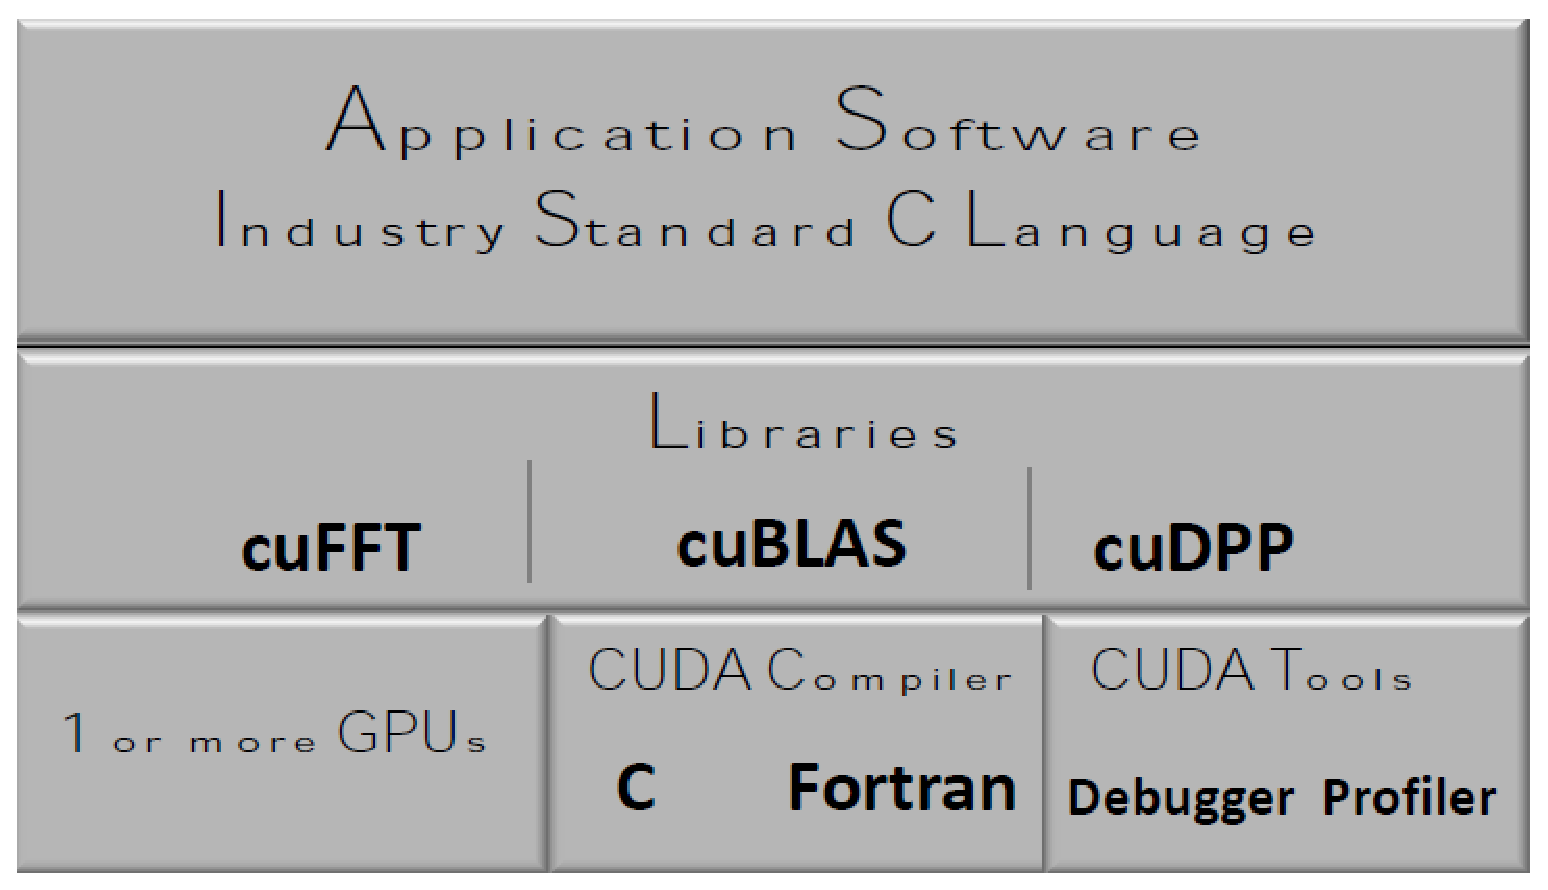
\includegraphics[height=5cm,
    angle=0]{./images/cuda_architecture.eps}}
\caption{CUDA architecture}
\label{fig:cuda_arch}
\end{figure}

CUDA C is a programming model that add some annotations (C-based extension) to
the C language for programmers to write code runnnig on GPU. Information on how to write 
programs running on Nvidia GPU is in Sect.\ref{sec:cuda-code}.

CUDA C can be divided into three components:
\begin{itemize}
\item CUDA libraries: required to run a CUDA application
  (\verb!cuda! core library, \verb!cudart!  runtime library)

\item CUDA toolkit (Sect.~\ref{sec:compile-tools-CUDA}): which provides 

a collection of tools required to develop a CUDA application (debugger,
profiler, driver tool (i.e. \hyperref[sec:nvcc]{nvcc})),

and optionally CUDA-enabled packages that provide commonly used functions so
that users doesn't have to rewrite them, e.g. (\hyperref[chap:cufft]{cuFFT},
\hyperref[chap:cublas]{cuBLAS}, \hyperref[chap:cudpp]{cuDPP}).

\item CUDA SDK (Software-Development Kit): samples that provide a starting point
for programmers in developing CUDA applications (read
Chap.~\ref{chap:cuda-sdk-sample}).
\end{itemize}

To help writing/evoking code to run on GP-GPU, specifically the GPU architecture
developed by Nvidia, Nvidia developped 
\begin{itemize}
  \item evoking code (.c/.cxx/.C): 
  
You have a regular C/C++ program (running on x86 CPUs), and then from there, you
can evoke CUDA {\bf kernel}.
  
  \item writing code to run on GPU (.cu file, or can be in .c/.cxx/.C file as
  well): this is called a {\bf kernel} in CUDA concept.
  
\end{itemize}
To compile both these C/C++ host code and kernel code,  CUDA provides the new
compiler tools, e.g. \verb!nvcc! (Sect.\ref{sec:nvcc}) that can recognizes, not
only existing C-host-code, but also support a new syntax - an extension to C
language standard to generate functions that can be run on Nvidia's GPGPU using
\verb!licudart! library.

In addition, Nvidia provides a set of APIs based on C language, that can
interact with CUDA GPUs, are implemented and provided to users in the form of
library \verb!libcudart.so!. Further collection of APIs are provided in other
libraries.


References:
\begin{enumerate}
\item \url{http://www.nvidia.com/cuda}
\item \url{http://www.gpgpu.org/developer/cudpp/}
\item \url{http://www.thalesians.com/finance/index.php/Knowledge_Base/CUDA/Installation}
\end{enumerate}

\subsection{Installing}
\label{sec:installing}

Installing CUDA library would include installing Nvidia graphics driver
(Sect.\ref{sec:nvidia-graphics_driver}), CUDA toolkit
(Sect.\ref{sec:install-toolkit}), and the CUDA SDK (Sect.\ref{sec:install-sdk}).

There are different version of CUDA (Sect.\ref{sec:cuda-toolkit}). However,
the general steps is as follows (order is important):
\begin{enumerate}
\item check the system (Sect.\ref{sec:check-system})
\item install Nvidia display driver (Sect.\ref{sec:nvidia-graphics_driver})
\item install CUDA toolkit (Sect.\ref{sec:install-toolkit})
\item install SDK (optional, part of the CUDA Toolkit package from CUDA 5.5) - Sect.\ref{sec:CUDA_55}
\end{enumerate}


\subsection{Check the system}
\label{sec:check-system}

% \begin{verbatim}
% lspci | grep -i nvidia
% \end{verbatim}

We may want to update the database
\begin{verbatim}
>> update-pciids

>> /sbin/update-pciids
\end{verbatim}

Check for CUDA-capable card
\begin{verbatim}
>> lspci | grep -i nvidia

>> lspci -vnn | grep -i VGA -A 12

01:00.0 VGA compatible controller [0300]: NVIDIA Corporation GT218 [GeForce 8400 GS Rev. 3] [10de:10c3] (rev a2) (prog-if 00 [VGA controller])
...
Kernel driver in use: nvidia
\end{verbatim}

Check for 32-bit or 64-bit CPU
\begin{verbatim}
uname -m 
\end{verbatim}
it will give you \verb!i386! or \verb!i686! for 32-bit and
\verb!x86_64! for 64-bit.

Check gcc:
\begin{verbatim}
gcc --version
\end{verbatim}

As nVidia graphics drivers are binaries, compiled with a particular version of
\verb!gcc!; the ABI of the gcc of the system must be compatible with those used
to compiled CUDA and nVidia driver.  A CUDA library requires a minimum version of
nVidia graphics drivers and support a maximum version of gcc
(Sect.\ref{sec:gcc_version}).

\begin{framed}
  API describes names of functions, types of parameters, their
  order... ABI (Application Binary Interface) describes size of
  structures, padding, order of fields in structures, mangling of names
  of methods..
\end{framed}

Check for OS
\begin{verbatim}
uname -r && cat /etc/*release
\end{verbatim}


\subsection{Install Nvidia graphics (NVIDIA display) driver}
\label{sec:nvidia-graphics_driver}

To 'talk' with a GPU device, we need a driver, i.e. a set of functions that the
device can understand.  Download the latest driver from nVidia website. Nowadays, install the toolkit
also install the CUDA driver. 

Download the CUDA toolkit (Sect.\ref{sec:install-toolkit}), as the toolkit also
contains the CUDA driver and tools needed to create/build/run a CUDA application.

Depending upon the CUDA toolkit's version, it is recommended
\begin{itemize}
\item CUDA 2.1 works with nVidia driver 180.xxx (Ubuntu 8.04)
\item CUDA 2.3 works with nVidia driver 190.xxx (Ubuntu 9.04)
\item CUDA 3.1 works with nVidia driver 256.xxx (Ubuntu 9.10)
\item CUDA 3.2 and above - recommended for Fermi - works with nVidia 260 or
later (doesn't work with nVidia 256)
\item CUDA 4.0 ???
\item CUDA 4.1 ???
\item CUDA 4.2: NVIDIA driver 295.41+
\item CUDA 5.0: NVIDIA driver 304.54 (minimum)
\item CUDA 5.5: NVIDIA driver 319.37+
\item CUDA 6.0: NVIDIA driver 331.62+
\item CUDA 6.5: NVIDIA driver 340.21+

\item CUDA 9.2:  NVIDIA driver 396.26+

\item CUDA 10.0:  NVIDIA driver 410.48+

\item CUDA 10.1:  NVIDIA driver 418.39+
\end{itemize}


A nVIDIA driver has 2 parts: kernel module
(Sect.\ref{sec:nvidia-driver-kernel-module}) and X11 driver (for graphical
display purpose). CUDA C requires the kernel module to run a CUDA program.

A given CUDA driver's version may require
\begin{enumerate}
   
  \item the presence of the Nvidia GPU (device compute) - Sect.\ref{sec:check-system}
  
  \item certain CPU architecture (host compute), e.g. PowerPC (ppc64), \verb!x86_64!
  
  \item certain  O/S, e.g. RedHat7 64-bit, Ubuntu 16.04 64-bit:
  
  \item certain version of the O/S kernel
  
\begin{verbatim}
uname -m && cat /etc/*release
\end{verbatim}  

   \item certain version of gcc compiler
   
\begin{verbatim}
gcc --version
\end{verbatim}

   \item the kernel header(s) is present and development packages are installed
   
\begin{verbatim}
uname -r

//Ubuntu
sudo apt-get install limux-headers-$(uname -r)

//RedHat  (use yum),  Fedora (use dnf)
sudo yum install kernel-devel-$(uname -r)  kernel-headers-$(uname -r)

// OpenSUSE/ SLES
// suppose 'uname -r' returns   3.16.6-2-default
// <variant>  = default
// <version>  = 3.16.6-2 

sudo zypper install -v kernel-<variant>-devel=<version>


\end{verbatim}

\end{enumerate}

There are two types of nVIDIA display driver: free and
proprietary\footnote{\url{http://wiki.debian.org/NvidiaGraphicsDrivers}}.

\begin{itemize}
\item free: 2 options (\verb!vesa! and \verb!nv! (better))

  Since Debian 6.0 (`Squeeze'): it has a new free driver
  \verb!nouveau! which is a reverse-engineered for nVIDIA cards (under
  development).
  
\item nvidia-current (from Ubuntu): to use this, this the end of the section.
\begin{verbatim}
 apt-get install nvidia-common nvidia-current
\end{verbatim}

\item proprietary (\textcolor{red}{recommended}): developed and managed by
nVidia. You need to remove
\begin{verbatim}
sudo  apt-get remove nvidia-common nvidia-current
\end{verbatim}
\end{itemize}

You're recommended to use proprietary driver (download from nVidia website).
CUDA driver comes with the nVidia proprietary display driver.
\begin{itemize}
  \item MAC O/S: \url{http://www.nvidia.com/object/mac-driver-archive.html}
  \item Unix/Linux: \url{http://www.nvidia.com/object/unix.html}
  \item Windows: \url{http://www.nvidia.com/Download/Find.aspx?lang=en-us}
\end{itemize}


\begin{mdframed}
Since Sept 2011, NVIDIA has created a new branch of their proprietary Linux
graphics driver, named {\bf long-lived} series. The purpose is to provide just
bug-fixes and other minor updates for non-legacy hardware (those are still
not old). There will be no new function added for long-lived series
\footnote{\url{http://www.phoronix.com/scan.php?page=news_item&px=OTkxOA}}. 
\url{http://www.nvidia.com/object/unix.html}

\end{mdframed}

After deciding which proprietary Nvidia driver to install, first you remove any
Ubuntu-provided nvidia graphics driver
\begin{verbatim}
apt-get --purge remove nvidia-*
\end{verbatim}

Next, we follows the instruction in 
\verb!/usr/share/doc/NVIDIA_GLX-1.0/README.txt!, i.e.

\begin{enumerate}
  \item To check if X-server is running
\begin{verbatim}
ps -e | grep X
\end{verbatim}

  \item turn off X-server
  
KILL all VNC server sessions:
\begin{verbatim}
sudo service vncserver stop
\end{verbatim}

Shutdown X server (if you have a Desktop version, press Alt-F1 upto
Alt-F6 to switch to the console interface, login and type)
\begin{verbatim}
  //Ubuntu
sudo killall gdm   
/etc/init.d/gdm stop

 // Xubuntu (xfce) rather than Ubuntu
/etc/init.d/xdm stop

  // Ubuntu 12.04+
service lightdm stop

  // Redhat (use Sys-V init system)
sudo /sbin/init 3
\end{verbatim}

\item Install 32-bit or 64-bit driver (depending on machine)
\begin{verbatim}
! 32-bit
sudo /cuda/NVIDIA-Linux-x86-177.67-pkg1.run  
! x86_64
sudo /cuda/NVIDIA-Linux-x86_64-177.67-pkg1.run
\end{verbatim}

You may want to add \verb!--update! option if you want to download the
latest driver version. 
% Latest\footnote{\url{http://www.nvidia.com/Download/index5.aspx?lang=en-us}}:
% \verb!/cuda/NVIDIA-Linux-x86_64-195.36.15-pkg2.run! to be able to use
% CUDA 3.0. 

\item Restart X server
\begin{verbatim}
  //Ubuntu
sudo /etc/init.d/gdm start

  // Since Ubuntu 12.04
service lightdm stop

  //Redhat
sudo /sbin/init 5
\end{verbatim}
\end{enumerate}


\begin{framed}
WHQL-certified (Windows Hardware Quality Labs) softwares are those which passed
Microsoft's testing process. Microsoft then issues a digitally signed
certification that can be included in the setup file to avoid
displaying a warning message when the software is
installed\footnote{\url{http://en.wikipedia.org/wiki/WHQL_Testing}}. The first
release from Nvidia drivers to be WHQL-certified:
\begin{itemize}
  \item GeForce 285.62:
  \url{http://www.nvidia.com/object/win7-winvista-64bit-285.62-whql-driver.html}
  \item R295 family: GeForce 295.73, GeForce 296.10 (add support GTX 560
  SE)\footnote{\url{http://fudzilla.com/home/item/26321-nvidia-geforce-29610-whql-drivers-released}}
  \item R300 family: GeForce
  301.42\footnote{\url{http://www.techspot.com/news/48705-geforce-30142-whql-packs-performance-gains-new-features.html
  }}
\end{itemize}
\end{framed}

References:
\begin{enumerate}
  \item \url{http://forums.nvidia.com/index.php?showtopic=198030}
\end{enumerate}


\subsection{-- 340.32}

\verb!libvdpau! and \verb!libvdpau_trace! (available separately via
\verb!libvdpau! project)
\footnote{\url{http://people.freedesktop.org/~aplattner/vdpau}}

\subsection{-- Nvidia CUDA-capable cards}
\label{sec:cuda_gpu}


Let's discover what kinds of Nvidia GPU support CUDA and how they are
different from each other. In this section, we introduce 3 strains of
CUDA-capable card from Nvidia: Geforce (high-end user - gaming),
Quadro (commercial - visual computing) and Tesla (scientific - high
performance computing (HPC)).
\begin{itemize}
\item Geforce is specifically designed for entertainment.
  \begin{enumerate}
  \item 1st gen (CC1.0, 1.1)\footnote{CC = Compute Capability (to be
      discussed later)}: CC1.0 = G80 architecture, CC1.1=G8x, e.g. Geforce GTX 
      8800 
  \item 2nd gen (CC1.3): Geforce GTX 280
  \item 3rd gen (CC2.0): Geforce GTX 470, GTX 480
  \end{enumerate}
\item Quadro is specifically designed for visual computing
  \begin{enumerate}
  \item 1st gen: Quadro FX 5600
  \item 2nd gen: Quadro FX 5800
  \item 3rd gen: Quadro FX 5900
  \end{enumerate}
\item Tesla is specifically designed for HPC, i.e. without VGA/DVI
  output, as shown in Fig.~\ref{fig:Nvidia_tesla}. However, Fermi has
  DVI output.
  \begin{enumerate}
  \item 1st gen (chip G80): C870 and S870 $\rightarrow$
    single-precision only.
  \item 2nd gen (Tesla T10 - use chip GT200): C1060 and S1070
    $\rightarrow$ support both single-precision and double-precision.
  \item Fermi (Tesla T20 - use chip GF100): C2050,
    C2070 - 7x faster for double-precision and many more enhancements.
  \end{enumerate}
\end{itemize}

Different strains, with different application purposes, have different
processor clocks, memory configurations and computing
features. However, those of the same generation all share some commons
in architecture which will be discussed in
Sect.~\ref{sec:gpu-unif-arch}.

\begin{figure}[hbt]
  \centerline{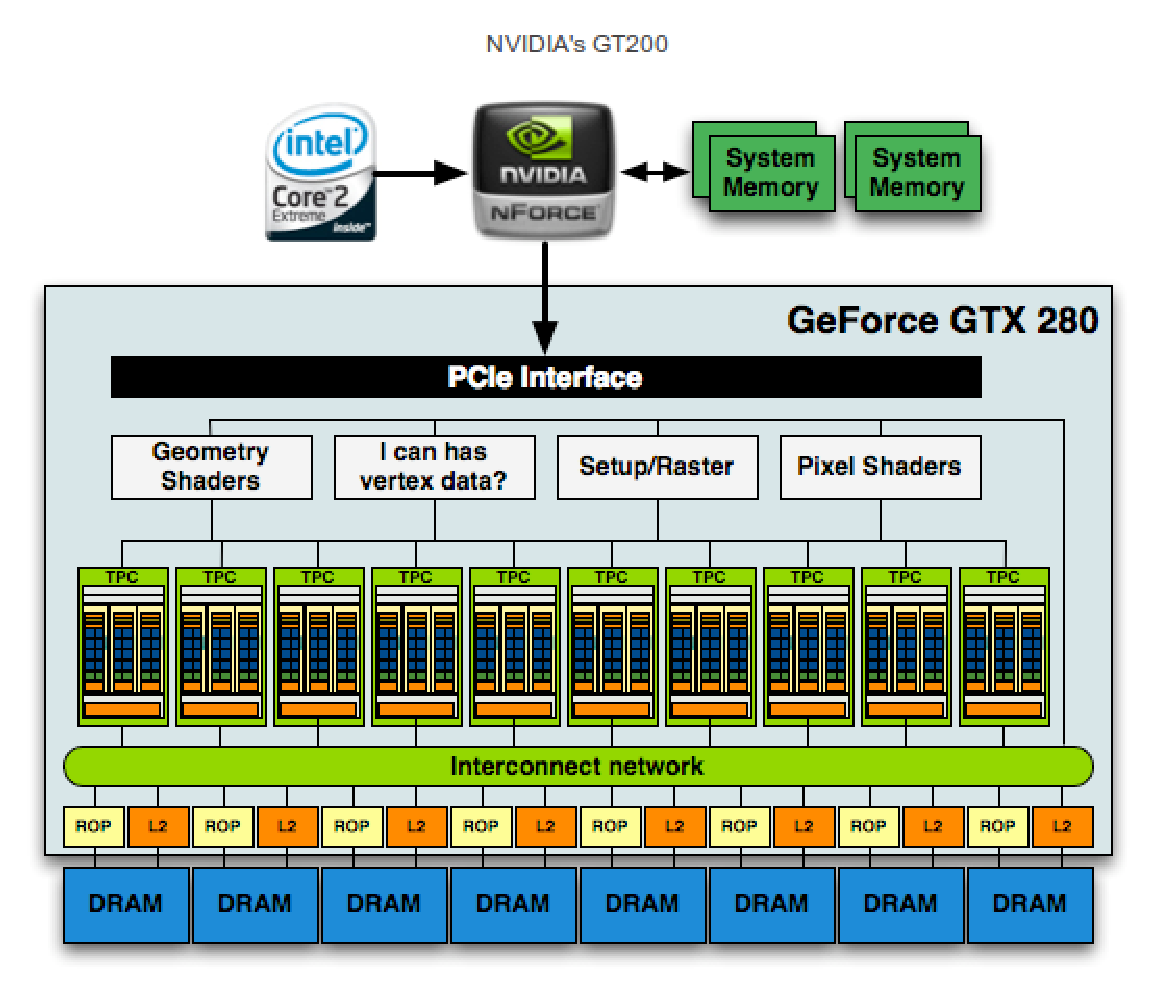
\includegraphics[height=8cm,
    angle=0]{./images/gtx200.eps}}
  % angle=0]{./images/Nvidia_tesla.eps}}
  \caption{General architecture of a Tesla 2nd gen}
  \label{fig:Nvidia_tesla}
\end{figure}


\begin{figure}[hbt]
  \centerline{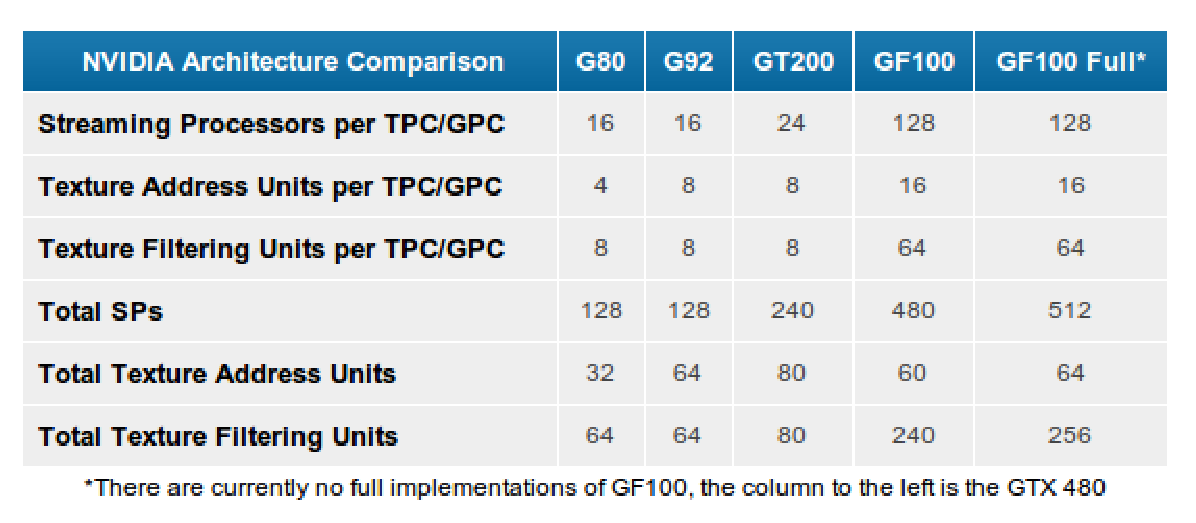
\includegraphics[height=5cm,
    angle=0]{./images/info_tesla_fermi.eps}}
  \caption{Nvidia Architecture comparison}
  \label{fig:info_tesla_fermi}
\end{figure}

GT80/GT92 use 90 nm TSMC technological process. GT92b use 55 nm
process\footnote{\url{http://alasir.com/articles/Nvidia_fermi_architecture/}}.
GT200 use 65 nm TSMC technology. GT200b or GT206 use 55 nm
technology. Even though GF100 use 40 nm technological process, its
limitation still does not allow full implementation of GF100, i.e. not
all 512 SPs are available,
Fig.~\ref{fig:info_tesla_fermi}.
\textcolor{red}{GTX480 have 480 cores per chip. Fermi
is based on GTX 470; thus has 448 cores.} GF110 have 512 functioning cores;
  yet it's double-precision processing power is lower than Fermi card.

\begin{framed}
  The future GPU, {\it codename ``Kepler''}, will be based on 28 nm technology,
  released in 2012. Kepler is believed to bring
  performance up to 3x to 4x higher than Fermi. The next
  generation, {\it codename ``Maxwell''} to be released in 2015, using 22 nm
  technology, is believed to bring 8x speedup compared to Fermi.
\end{framed}


\subsection{-- CUDA driver kernel module}
\label{sec:nvidia-driver-kernel-module}


Kernel module is one of the two part of a nVIDIA graphics driver.
The NVIDIA kernel mode driver must be running and connected to a target GPU
device before any user interactions with that device can take place.

\begin{enumerate}
  \item  On Windows the kernel mode driver is loaded at Windows startup and kept loaded until Windows shutdown.
  
  \item Under Linux systems where X runs by default on the target GPU the kernel mode driver will generally be initalized and kept alive from machine startup to shutdown, courtesy of the X process
  
  \item On headless systems or situations where no long-lived X-like client maintains a
handle to the target GPU, the kernel mode driver will initilize and deinitialize
the target GPU each time a target GPU application starts and stops.
  
  Since it is often desireable to keep the GPU initialized in these cases,
  NVIDIA provides two options for changing driver behavior: Persistence Mode
  (Legacy) and the Persistence Daemon.
  
\end{enumerate}



\subsection{Install CUDA toolkit}
\label{sec:install-toolkit}

In the early version of CUDA, we need to install CUDA driver
(Sect.\ref{sec:nvidia-graphics_driver}), CUDA SDK (Sect.\ref{sec:install-sdk}),
and CUDA toolkit using two separate files. 

Nowadays, install the toolkit also install the CUDA driver, to ensure you have a
working system. However, we need to make sure the system is ready to install
that (Sect.\ref{sec:nvidia-graphics_driver}). Example: as the CUDA Toolkit needs
to be compiled on your machine, it is important to have the right gcc version
that work with the CUDA Toolkit version. This depends on the Ubuntu version
being used (Sect.\ref{sec:troubleshoot_Ubuntu_version}).

The higher version of the CUDA toolkit, the newer GPU that it supports.
Depending on the CUDA-capable GPUs in the system, we select the appropriate
version of the CUDA toolkit as the toolkit contains tools required to compile a
CUDA program.


NOTICE:
 \begin{itemize}
 \item You need to use CUDA 3.0 toolkit or above if you have Fermi GPU.
 
 \item You need to use CUDA 5.0 toolkit or above if you have Kepler GPU.
   
 \item Install NVIDIA 32-bit compatibility OpenGL libraries also.

 \item If you want to install multiple versions of the CUDA toolkit on a single
   machine, install it to the folder with the version name,
   e.g. \verb!/usr/local/cuda30/!, \verb!/usr/local/cuda23/!, and link
  \begin{verbatim}
  ln -s /usr/local/cuda30 /usr/local/cuda
  \end{verbatim}
  when you use one.
  
  UPDATE: From CUDA 5.5, the name pattern for CUDA folder is
  \verb!cuda-<major>.<minor>!, e.g.
  \begin{verbatim}
  /usr/local/cuda-5.5
  /usr/local/cuda-6.0
  \end{verbatim}
  
\end{itemize}


\begin{enumerate}

   \item Link to download:

\url{https://developer.nvidia.com/cuda-downloads?target_os=Linux&target_arch=ppc64le&target_distro=Ubuntu&target_version=1804&target_type=deblocal}

NOTICE: On Power9 machine - Sect.\ref{sec:power9-CUDA}

\item Kill any running X server (optional)

\item Login the machine using console, and install the toolkit


Nowadays: download the deb (network) version
\begin{verbatim}

//network deb
`sudo dpkg -i cuda-repo-ubuntu1604_9.2.148-1_ppc64el.deb`
`sudo apt-key adv --fetch-keys http://developer.download.nvidia.com/compute/cuda/repos/ubuntu1604/ppc64el/7fa2af80.pub`
`sudo apt-get update`
`sudo apt-get install cuda`

// to install all the library packages, replace "cuda" with the "cuda-libraries-9-2" meta packag
`sudo apt-get install cuda-libraries-9-2`

//local deb

`sudo dpkg -i cuda-repo-ubuntu1804-10-0-local-10.0.130-410.48_1.0-1_ppc64el.deb`
`sudo apt-key add /var/cuda-repo-<version>/7fa2af80.pub`
`sudo apt-get update`
`sudo apt-get install cuda`
sudo apt-get install cuda-drivers
\end{verbatim}


The recommended installation package is the cuda package (the compiler, the
debugger, the profiler, the math libraries,). This package will install the full
set of other CUDA packages required for native development and should cover most
scenarios.

\url{https://docs.nvidia.com/cuda/cuda-installation-guide-linux/index.html}


Old versions:
\begin{verbatim}
! 32-bit
sudo /cuda/cudatoolkit_2.1_linux32_ubuntu8.04.run
! x86_64
sudo /cuda/cudatoolkit_2.1_linux64_ubuntu8.04.run
\end{verbatim}
 The default location to install to is \verb!/usr/local/cuda!.

NOTE: From CUDA 5.5, the CUDA SDK comes with the CUDA Toolkit in the same
package, so you may get the error when installing the package. Read
Sect.\ref{sec:install-sdk} for troubleshooting. If you use the wrong gcc
version, you may get the error
\begin{verbatim}
Toolkit:  Installation Failed. Using unsupported Compiler.
Samples:  Installation Failed. Missing required libraries.
\end{verbatim}


\item Restart X server
\end{enumerate}

You should add/update the following two environment variables (in
\verb!~/.bashrc! or \verb!~/.profile!)
\begin{verbatim} 
* Please make sure your PATH includes /usr/local/cuda/bin
* Please make sure your LD_LIBRARY_PATH includes /usr/local/cuda/lib
If your machine is 64-bit, use /usr/local/cuda/lib64 instead.
\end{verbatim}
or adjust it to the correct path if your system install multiple
versions of CUDA. An alternate way if you have \verb!root! privilege, you just
create /etc/ld.so.conf/cuda.conf
\begin{verbatim}
/usr/local/cuda/lib64
/usr/local/cuda/lib
\end{verbatim}
and then run
\begin{verbatim}
sudo ldconfig
\end{verbatim}


\subsection{Install CUDA SDK}
\label{sec:install-sdk}

In earlier versions of CUDA, this is not requirement but is recommended as the
SDK contains sample codes in CUDA C.
From CUDA 5.5, the CUDA SDK is part of the CUDA Toolkit installation package.
So, the troubleshooting below should be applied when you see the problems with
installing CUDA Toolkit 5.5 and above.

In a multi-user system, each user should install in their own home
folder for personal use.
\begin{verbatim}
cd ~
/cuda/NVIDIA_CUDA_sdk_2.0beta2_linux.run
\end{verbatim}
% Latest: \verb!gpucomputingsdk_3.2RC_linux.run!. 
We can download from CUDA zone. 
For each version of
CUDA, you're advised to maintain two different version of SDK, one for
32-bit and one for 64-bit machine, e.g.
\verb!~/NVIDIA_CUDA_SDK_2.3-x86! and
\verb!~NVIDIA_CUDA_SDK_2.3-x86_64!.

When using \verb!nvidia-current!, the library \verb!libcuda.so! is by default
located in \verb!/usr/local/nvidia-current! and \verb!ld! tool cannot detect
this. To be able to compile the SDK, we need to change the line 278 of
SDK/C/common/common.mk to
\begin{verbatim}
   LIB += -L/usr/lib/nvidia-current -lcuda   ${OPENGLLIB} $(PARAMGLLIB) 
                  $(RENDERCHECKGLLIB) $(CUDPPLIB) ${LIB}
\end{verbatim}

CUDA 4.0: when you compile the CUDA SDK, you may get the following
error
\begin{verbatim}
    -lXi  -lglut -lXmu
\end{verbatim}
then you need to open \verb!aptitude! and search for ``libXi'', ``libglut'' and
``libxmu'', which return \verb!libxi-dev!, \verb!libglut3-dev! (NOTE:
\verb!libglut3-dev! has been replaced by \verb!freeglut3-dev! in Ubuntu 11.10)
and \verb!libxmu-dev!. Install these packages, as well as their dependencies.

In CUDA 4.0, when you compile your SDK on Ubuntu 11.04 and 11.10 which
use gcc/g++ higher than version 4.4, to resolve this, read
Sect.\ref{sec:troubleshoot_Ubuntu_version}.

CUDA 4.1 works with Ubuntu 11.04.

Since CUDA 5.0, we see some changes 
\begin{enumerate}
  \item The locations of the installation folder: the default is
  /usr/local/cuda-5.0, rather than /usr/local/cuda.
  \item The location of the SDK is /usr/local/cuda-5.0/samples, rather than
  /usr/local/NVIDIA\_GPU\_Computing\_SDK.
  \item  Also, a single installation file contains 3 components: Nvidia driver +
  CUDA driver + CUDA SDK. 
\end{enumerate}

In Ubuntu 12.04, the location of \verb!libglut.so! library is
/usr/lib/x86\_64-linux-gnu/, rather than /usr/lib/. Thus, installing the SDK may
gives you the error
\begin{verbatim}
Missing required library libglut.so
\end{verbatim}
The reason is that Ubuntu x64 uses a different path. To resolve this problem,
run

\begin{verbatim}
sudo ln -s /usr/lib/x86_64-linux-gnu/libglut.so /usr/lib/libglut.so
#Ubunt 32-bit:
sudo ln -s /usr/lib/i386-linux-gnu/libglut.so.3 /usr/lib/libglut.so
#Cent OS 5.6 x64 or Fedora
yum install freeglut
ln -s /usr/lib/libglut.so.3 /usr/lib/libglut.so
\end{verbatim}

To compile CUDA 5.0 SDK, it may ask for mpicxx
\begin{verbatim}
MPI not found, not building simpMPI
\end{verbatim}
to resolve, we install
\begin{verbatim}
apt-get install libmpich2-dev
\end{verbatim}


References:
\begin{itemize}
  \item \url{http://developer.nvidia.com/cuda-toolkit}
  \item \url{http://forums.nvidia.com/index.php?showtopic=198030}
\end{itemize}

\subsection{Select GCC version}
\label{sec:gcc_version}

As nVidia graphics drivers are binaries, compiled with a particular version of
\verb!gcc!; the ABI of the libstdc, libstdc++ version of gcc of the system must
be compatible with those used to compiled CUDA and nVidia driver. 

A CUDA library requires a minimum version of nVidia graphics drivers and support
a maximum version of gcc, i.e.
\begin{itemize}
  \item should be 4.3.4 for CUDA 2.3 and CUDA 3.0.
  \item should be 4.4 for CUDA 4.0 and 4.1.
  \item should be 4.6 for CUDA 5.0 (not supporting gcc 4.7)
  \item should be 4.7.2 or below for CUDA 5.5 (not supporting gcc 4.7.3)
  \item should be 4.8 for CUDA 6.x
\end{itemize}

\begin{framed}
Higher versions of CUDA work with lower version of Ubuntu, given the
appropriate nVidia drivers. Lower version of CUDA may not work with
higher version of Ubuntu, as the default version of \verb!gcc! is not
ABI compatible with the one used to compile CUDA. The reason is that different
versions of Ubuntu are compiled with different versions of gcc.
We can check NVIDIA Driver version
\begin{verbatim}
cat /proc/driver/nvidia/version 
\end{verbatim}
\end{framed}


To install g++-4.7
\begin{verbatim}
sudo add-apt-repository ppa:ubuntu-toolchain-r/test
sudo apt-get update
sudo apt-get install gcc-4.7 g++-4.7
\end{verbatim}

then to switch between 4.6 or 4.7 we do
\begin{verbatim}
sudo update-alternatives --install /usr/bin/gcc gcc /usr/bin/gcc-4.6 60 --slave /usr/bin/g++ g++ /usr/bin/g++-4.6 
sudo update-alternatives --install /usr/bin/gcc gcc /usr/bin/gcc-4.7 40 --slave /usr/bin/g++ g++ /usr/bin/g++-4.7 
sudo update-alternatives --config gcc
\end{verbatim}
However, there are different minor versions. For example: gcc 4.7 in Ubuntu
13.10 is indeed 4.7.3; while CUDA 5.5. can be compiled by gcc upto 4.7.2. Thus
we need to use a lower version, i.e. 4.6.

\subsection{Troubleshooting}
\label{sec:troubleshooting-1}

\subsection{-- CUDA 2.3}

\begin{itemize}
\item CUDA 2.3. only work with NVIDIA driver from 190.xx. So, you
  should check and update the latest NVIDIA driver.

\item CUDA 2.3 mainly work with gcc 4.3, it has some problems with gcc
  4.4.x. with weak link error.
\end{itemize}

{\bf Workaround gcc-4.4.x with CUDA 2.3}
\begin{enumerate}
\item [Try 1] Here is one way to work around, edit the file
  \verb!common.mk!  and add one more flag to \verb!NVCCFLAGS!.
\begin{verbatim}
NVCCFLAGS += --compiler-options -fno-inline
\end{verbatim}

\item [Try 2] If try 1 doesn't work, recover \verb!common.mk!, and
  override NVCCFLAGS -O2 with -O0 or null.

\item [Try 3] (Ubuntu 9.10) uninstall gcc/g++ 4.4, install gcc/g++
  4.3, and manually link of /usr/bin/gcc to /usr/bin/gcc-4.3, and same
  for g++.
  \begin{verbatim}
  ln -s /usr/bin/gcc-4.3 /usr/bin/gcc
  ln -s /usr/bin/g++-4.3 /usr/bin/g++
  \end{verbatim}

\item [Try 4] (Ubuntu 9.10) You can modify the \verb!common.mk! by
  changing -O2 like this
\begin{verbatim}
diff common/common.mk common/common.mk.org
159c159
<     COMMONFLAGS +=
---
>     COMMONFLAGS += -O2
162,164c162,164
<     CXXFLAGS    += -fno-strict-aliasing -O2
<     CFLAGS      += -fno-strict-aliasing -O2
---
>     CXXFLAGS    += -fno-strict-aliasing
>     CFLAGS      += -fno-strict-aliasing
\end{verbatim}

\item [Try 5] If you want to keep multiple versions of gcc/g++ on the machine,
  one way is
  \begin{enumerate}
  \item compile the CUDA code with nvcc and gcc 4.3,
  \item compile the rest with gcc.4.4 or gcc 4.5 and link with (1)
  \end{enumerate}

  How to switch between versions of gcc on the machine
\begin{verbatim}
sudo update-alternatives --install /usr/bin/gcc gcc 
   /usr/bin/gcc-4.1 60 
   --slave /usr/bin/g++ g++ /usr/bin/g++-4.1

sudo update-alternatives --install /usr/bin/gcc gcc 
  /usr/bin/gcc-4.2 40 
  --slave /usr/bin/g++ g++ /usr/bin/g++-4.2
\end{verbatim}
  that sets gcc-4.1 and g++-4.1 as default (i.e. gcc now points to
  gcc-4.1), and you can easily select the gcc version you want to use with
\begin{verbatim}
sudo update-alternatives --config gcc
\end{verbatim}
\end{enumerate}


\subsection{-- CUDA 3.x}

\begin{itemize}
\item CUDA 3.0 mainly work with gcc 4.3, it has some problems with gcc
  4.4.x. with weak link error.
  \textcolor{red}{Ubuntu 9.10 comes with gcc 4.4.1, thus you're
    recommended to use Ubuntu 9.04 for CUDA 2.3/3.0}.
\end{itemize}

{\bf Workaround gcc-4.4.x with CUDA 3.0 in Ubuntu 9.10}:
\begin{enumerate}
\item Install gcc-4.3, besides gcc 4.4.1
\begin{verbatim}
sudo apt-get install g++-4.3 gcc-4.3
\end{verbatim}
\item Make a copy of the \verb!common.mk! file 
\item Change all \verb!gcc! in the file to \verb!gcc-4.3!
\item Change NVCCFLAGS to
\begin{verbatim}
NVCCFLAGS := --compiler-options -fno-inline --compiler-bindir=/usr/bin/g++-4.3
\end{verbatim}
  or 
\begin{verbatim}
NVCCFLAGS := --compiler-options -fno-inline --compiler-bindir=/opt/gcc-4.3
\end{verbatim}

\end{enumerate}
% \begin{enumerate}
% \item [Try 1] patch the \verb!common.mk! file
% \begin{verbatim}

% --- pkg/sdk/C/common/common.mk 2010-03-03 22:14:46.000000000 +0900
% +++ pkg/sdk/C/common/common.mk.fix 2010-03-29 20:39:15.000000000 +0900
% @@ -55,7 +55,7 @@
% SHAREDDIR := $(ROOTDIR)/../../shared/

% # Compilers
% -NVCC := $(CUDA_INSTALL_PATH)/bin/nvcc
% +NVCC := nvcc
% CXX := g++
% CC := gcc
% LINK := g++ -fPIC
% @@ -89,7 +89,7 @@
% # architecture flag for nvcc and gcc compilers build
% CUBIN_ARCH_FLAG :=
% CXX_ARCH_FLAGS :=
% -NVCCFLAGS :=
% +NVCCFLAGS := --compiler-options -fno-inline
% LIB_ARCH := $(OSARCH)

% # Determining the necessary Cross-Compilation Flags
% \end{verbatim}
% \item go to sdk/C and call make. 
% \end{enumerate}

\subsection{-- CUDA 4.0}

From CUDA 4.0, an important issue is that in order to run CUDA
application, CUDA module need to be loaded and the entries in \verb!/dev! are
created. This is automatically  created if you have X windows, e.g. GNOME.

However, if you run a Ubuntu server,  this requires \verb!root! to run a CUDA
program every time you reboot the  machine, e.g. /deviceQuery. To avoid this,
you can create a script to load the kernel module and create the entries in
/dev. Suppose you have three device, it will create
\begin{verbatim}
/dev/nvidia0
/dev/nvidia1
/dev/nvidia2
/dev/nvidiactl
\end{verbatim}

The script, to be saved as \verb!/etc/init.d/cuda_init!, with content
\begin{verbatim}
#!/bin/bash

/sbin/modprobe nvidia

if [ "$?" -eq 0 ]; then

# Count the number of NVIDIA controllers found.
N3D=`/sbin/lspci | grep -i NVIDIA | grep "3D controller" | wc -l`
NVGA=`/sbin/lspci | grep -i NVIDIA | grep "VGA compatible controller" |
wc -l`

N=`expr $N3D + $NVGA - 1`
for i in `seq 0 $N`; do
mknod -m 666 /dev/nvidia$i c 195 $i;
done

mknod -m 666 /dev/nvidiactl c 195 255

else
exit 1
fi
\end{verbatim}

The script to be saved in /etc/init.d; then make it executable
\begin{verbatim}
chmod 755 /etc/init.d/cuda_init
\end{verbatim}
Add propriate symbolic links to make sure the script is evoked at boot time
\begin{verbatim}
update-rc.d cuda_init defaults
\end{verbatim}
If we no longer want, and to remove it, we use
\begin{verbatim}
update-rc.d -f cuda_init remove
\end{verbatim}
Here, the script is not removed, just the symbolic links are
removed\footnote{\url{http://www.debian-administration.org/articles/28}}.


NOTE: The problem above is resolved in CUDA 4.1.

\subsubsection{-- Misc. error}

If you get this error 
\begin{verbatim}
... FAILED CUDA Driver and Runtime version may be mismatch
\end{verbatim}
but not when you run the program as root; then you should call
\begin{verbatim}
setenforce 0
\end{verbatim}
or you may want to remove completely
\begin{verbatim}
sudo apt-get --purge remove nvidia-*
\end{verbatim}
restart the machine and reinstall again if using setenforce doesn't
work.

If you get this error
\begin{verbatim}
Runtime API error 10: invalid device ordinal
\end{verbatim}
make sure you use two 6-pin cable or one 8-pint cable, not one 6-pint cable for
the device\footnote{\url{http://forums.nvidia.com/index.php?showtopic=201963}}. 


\textcolor{red}{In Ubuntu 10.04 server}, you may get the error
\begin{verbatim}
The distribution-provided pre-install script failed
\end{verbatim}
A solution is to add \verb!-k $(uname -r)! to the command line
\begin{verbatim}
sudo /cuda/NVIDIA-Linux-x86_64-280.13.run -k $(uname -r)
\end{verbatim}
or a better solution (always work) is
\begin{enumerate}
\item download the latest nVidia driver
\item open module blacklist 
\begin{verbatim}
gedit /etc/modprobe.d/blacklist.conf
\end{verbatim}
add
\begin{verbatim}
blacklist vga16fb
blacklist nouveau
blacklist rivafb
blacklist nvidiafb
blacklist rivatv
\end{verbatim}
\item remove any previously installed nVidia drivers
\begin{verbatim}
apt-get --purge remove nvidia-*
\end{verbatim}
\item reboot, and go to terminal
\item run the latest downloaded nVidia driver
\begin{verbatim}
sudo /cuda/NVIDIA-Linux-x86_64-280.13.run 
\end{verbatim}

\item if an error message regarding \verb!nouveau! driver persistent, we just
run
\begin{verbatim}
sudo update-initramfs -u
\end{verbatim}
\end{enumerate}
which in Fedora/RedHat, we need to use \verb!dracut!. In Redhat/Fedora, we need
to
\footnote{\url{http://linux.xvx.cz/2011/01/nvidia-proprietary-drivers-and-rhel6/}}
\begin{enumerate}
  \item Ctrl-Alt-F2 : to switch to the terminal  
  \begin{verbatim}
yum update
yum install gcc kernel-devel
reboot
  \end{verbatim}
  \item Blacklist nouveau
\begin{verbatim}
sed -i '/root=/s|$| rdblacklist=nouveau vga=791|' /boot/grub/grub.conf
echo "blacklist nouveau" >> /etc/modprobe.d/blacklist.conf
\end{verbatim}
  \item Change initrd image
\begin{verbatim}
mv /boot/initramfs-$(uname -r).img /boot/initramfs-$(uname  -r)-nouveau.img
dracut /boot/initramfs-$(uname -r).img $(uname -r)
\end{verbatim}
and remove the nouveau driver
\begin{verbatim}
yum remove xorg-x11-drv-nouveau
reboot
\end{verbatim}
  \item \verb!sudo telinit 3!: to turn off the X-server
\begin{verbatim}
sudo telinit 3
init 3
chmod +x NVIDIA-Linux-x86-260.19.29.run
 ./NVIDIA-Linux-x86-260.19.29.run
\end{verbatim}
  \item \verb!sudo dracut -f /boot/initramfs-<currentimage>!: to update the
  kernel, with <currentimage> is the version of the kernel being used (or the
  one that you want to update).
  \item \verb!sudo reboot! or \verb!telinit 5!
\end{enumerate}

If you get the error
\begin{verbatim}
File /usr/lib/xorg/modules/extensions/libglx.so' is not a symbolic link
\end{verbatim}
then make a symbolic link
\begin{verbatim}
cd /usr/lib/xorg/modules/extensions
ln -s libglx.so.310.40 libglx.so
\end{verbatim}

References:
\begin{itemize}
\item
  \url{http://forums.nvidia.com/lofiversion/index.php?t104525.html}:
  Work around gcc 4.4.x for CUDA 2.3.
\item \url{http://forums.nvidia.com/index.php?showtopic=164598}: Work
  around gcc 4.4.1 for CUDA 3.0.
\item \url{https://visualization.hpc.mil/wiki/CUDA_3.0_error_messages}
\item \url{http://www.ubuntugeek.com/howto-install-nvidia-drivers-manually-on-ubuntu-10-04-lucid-lynx.html}
\end{itemize}

\subsection{-- CUDA 6.0 and 6.5}

CUDA 6.0 uses gcc version 4.8.1 (or older).

\subsection{-- CUDA 7.0}
\label{sec:CUDA-7.0-troubleshoot}

\subsection{-- Errors were encountered while processing:}

\begin{verbatim}
// database got corrupted 
sudo dpkg --configure -a

// force reinstall
sudo apt-get install -f

// remove the troublesome package
sudo apt remove 

// remove files associated with the package in 
/var/lib/dpkg/info.

ls -l /var/lib/dpkg/info | grep -i polar-bookshelf

\end{verbatim}
\subsection{-- Power9 and CUDA}
\label{sec:power9-CUDA}

On AC9222 Power9 machine, the firmware needs to be OP910.24 or OP920.02 to use 
CUDA 9.2 (9.2.148) - Sect.\ref{sec:CUDA_9.2}. 
\url{https://delivery04.dhe.ibm.com/sar/CMA/SFA/07jae/0/AC922_8335-GTG_OpenPowerReadme.v1.4.xhtml}

\url{https://www-945.ibm.com/support/fixcentral/swg/selectFixes?parent=Scale-out LC}

\subsection{Ubuntu versions}
\label{sec:troubleshoot_Ubuntu_version}

\subsection{-- Ubuntu 9.10+}

\textcolor{red}{In Ubuntu 9.10}, it uses gcc 4.4.1 which is incompatible with
CUDA 2.3. So, you may have problem when compiling your SDK or your CUDA
program, read the solution in Sect.~\ref{sec:troubleshooting-1}.

\subsection{-- Ubuntu 11.04, 11.10}


\textcolor{red}{In Ubuntu 11.04 and 11.10}, it use gcc 4.5 and 4.6,
correspondingly\footnote{\url{http://distrowatch.com/table.php?distribution=ubuntu}},
which are incompatible with CUDA 4.0. 

CUDA 4.1 work with Ubuntu 11.04, but not
with Ubuntu 11.10\footnote{\url{http://developer.nvidia.com/cuda-toolkit-41}}.

To work around, there are two options:
\begin{enumerate}
  \item Make nvcc use gcc/g++ 4.4: install gcc/g++ 4.4 then 
  \begin{verbatim}
  mkdir gcc44
  cd gcc44
  ln -s /usr/bin/cpp-4.4 cpp
  ln -s /usr/bin/gcc-4.4 gcc
  ln -s /usr/bin/g++-4.4 g++
  \end{verbatim}
  then we edit the file /usr/local/cuda/bin/nvcc.profile to look into this
  folder
  \begin{verbatim}
  compiler-bindir = /wherever/you/put/your/gcc44
  \end{verbatim}
  
  \item Make the whole system use gcc/g++ 4.4: use \verb!update-alternatives!
  command.
\end{enumerate}
\subsection{-- Ubuntu 12.04}

As of 6/05/2013, there is currently a release of gcc 4.8.1 for 12.04(precise)
available at \url{https://launchpad.net/~ubuntu-toolchain-r/+archive/test}

\begin{verbatim}
sudo apt-get install python-software-properties
sudo add-apt-repository ppa:ubuntu-toolchain-r/test
sudo apt-get update
sudo apt-get install gcc-4.8
sudo update-alternatives --install /usr/bin/gcc gcc /usr/bin/gcc-4.8 50
\end{verbatim} 


\subsection{-- Ubuntu 13.10}

\textcolor{red}{In Ubuntu 13.10}, it uses gcc 4.7 (4.7.3) which is incompatible
with CUDA 5.5. CUDA 5.5. works with gcc 4.7.2 and below. To work around, install
gcc 4.6 and use \verb!update-alternatives!
\begin{verbatim}
apt-get install gcc-4.6 g++-4.6

sudo update-alternatives --remove-all gcc
sudo update-alternatives --remove-all g++
sudo update-alternatives --install /usr/bin/gcc gcc /usr/bin/gcc-4.6 30
sudo update-alternatives --install /usr/bin/g++ g++ /usr/bin/g++-4.6 30
sudo update-alternatives --install /usr/bin/gcc gcc /usr/bin/gcc-4.7 20
sudo update-alternatives --install /usr/bin/g++ g++ /usr/bin/g++-4.7 20
sudo update-alternatives --install /usr/bin/gcc gcc /usr/bin/gcc-4.8 10
sudo update-alternatives --install /usr/bin/g++ g++ /usr/bin/g++-4.8 10
\end{verbatim}

Now, we can switch from one gcc version to another before installing CUDA
Toolkit/SDK with
\begin{verbatim}
sudo update-alternatives --config gcc 
\end{verbatim}
replace gcc with g++ to configure that if you want, too.
\url{https://n00bsys0p.co.uk/blog/2014/01/23/nvidia-cuda-55ubuntu-1310-saucy-salamander}

\subsection{-- Ubuntu 14.04}

\section{CUDA Toolkit: built tools (e.g. nvcc) + libraries (e.g. cudart.so)}
\label{sec:cuda-toolkit}

To help programming on GPU using CUDA programming model, Nvidia has developed
some libraries, sample codes, drivers (i.e. nvcc), etc. They form the so-called
CUDA toolkit. 

Since version 3.0, CUDA Toolkit are versioned and is installed in a separate
folder, i.e. users can select the appropriate CUDA Toolkit to use.

\sout{CUDA SDK is now (Jan, 2010) at version 2.3}. CUDA 2.3 supports Linux (32-
and 64-bit), Windows (32- and 64-bit) and Mac OS 10.5. \sout{CUDA SDK is now 3.1
(June, 2010)}. \sout{CUDA SDK is now 3.2 (Sept, 2010)}. 

CUDA 3.x is specifically designed to utilize the power of Fermi architecture. 
CUDA 3.0 is known to run slower than CUDA 2.3 on GPU CC 1.x. CUDA 3.1 resolves
such problems in CUDA 3.0 and fully support Fermi. \sout{CUDA SDK is now 4.0
(Aug, 2011)}.

CUDA 4.0 support GPUDirect 2.0 for multiple GPU within a single node
(Sect.\ref{sec:GPUs_GPUDirect2}), as well as new CUDA API memory management that
allows pageable memory to be used as pinned memory
(Sect.\ref{sec:cuda4_nocopy_pinning}).


Check Sect.\ref{sec:nvcc} to knows the compatible between CUDA toolkit version
and GNU gcc versions.

\subsection{CUDA APIs}
\label{sec:cuda-apis}

CUDA has a set of APIs at different level, as shown in
Fig.~\ref{fig:CUDA_API}. The lower the level, the higher the
flexibility (or the more functionality), yet the more complicated to
use. The highest one is some library written by Nvidia or third-party to use
(cuFFT, CUBLAS, CURAND), the second one is CUDA runtime API (which can be in C
(Chap.\ref{chap:c-cuda}), Fortran (Chap.\ref{chap:cuda-fortran}), Python, etc.),
the third and lowest-level is CUDA driver API (which now becomes part of the
OpenCL language standard).

\begin{figure}[hbt]
  \centerline{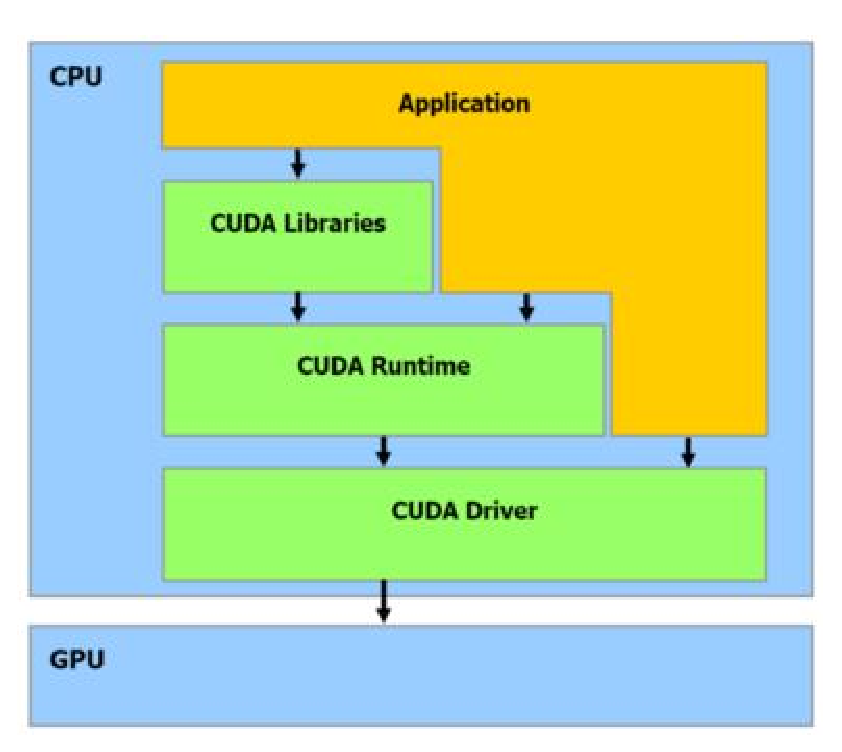
\includegraphics[height=6cm,
    angle=0]{./images/CUDA_API.eps}}
  \caption{CUDA API at different level}
  \label{fig:CUDA_API}
\end{figure}

Your application is allowed to call the API at any level; yet between CUDA
runtime API or CUDA driver API, only one level is available to use in a single
program, i.e. they are exclusive. 

\begin{enumerate}
\item CUDA driver API (lower-level), all entry points are prefixed
  with \verb!cu!, delivered through the \verb!nvcuda! dynamic library
  (see Chap.~\ref{chap:cuda-driver-api})
\item C runtime for CUDA (higher-level), prefix with \verb!cuda! (see
  Chap.~\ref{chap:c-cuda})
\end{enumerate}
Recently, we have Fortran runtime for CUDA (see
Chap.~\ref{chap:cuda-fortran}), which has the same syntax with C
runtime for CUDA; yet with some limitations in memory access.

In addition to CUDA C and CUDA Fortran, there are also extension to
other programming languages as well, e.g. CUDA
Fortran\footnote{\url{http://www.pgroup.com/resources/cudafortran.htm}},
PyCuda (Python), CUDA Matlab. Read Chap.~\ref{chap:c-cuda},
Chap.~\ref{chap:cuda-fortran}.  In the coming chapters, we will
discuss
\begin{itemize}
\item \hyperref[chap:c-cuda]{C CUDA}
\item \hyperref[chap:cuda-fortran]{Fortran CUDA}
\item \hyperref[chap:accel-progr-model]{APM}
\end{itemize}

\subsection{CUDA 2.1}

New:
\begin{enumerate}
  \item JIT compilation
  \item new interoperability APIs for Direct3D 9 and Direct3D 10 (to accelerate
  communication with DirectX applications)
  \item OpenGL interoperability improvements
  \item Debugger support using \verb!gdb! (RedHat 5.x)
  \item Support OS: Fedora9, OpenSUSE 11 and Ubuntu 8.04
\end{enumerate}

\subsection{CUDA 2.3}
\label{sec:CUDA_2.3}

\subsection{CUDA 3.0}
\label{sec:CUDA_3.0}

New:
\begin{enumerate}
\item CUDA Memory Checker: report misalignment and out of bound errors
  $\rightarrow$ use in cuda-gdp or a stand-alone utility. 

\item CUDA C/C++ kernels are compiled to standard ELF format (Sect.\ref{sec:ELF}). 

\item Support OpenCL in R195.39 beta driver

\item Early support for Fermi
\end{enumerate}

CUDA 3.0 is known for slower performance than CUDA 2.3. 

\subsection{CUDA 3.1}
\label{sec:CUDA_3.1}

Environment variables:
\begin{itemize}
\item \verb!CUDA_VISIBLE_DEVICES!: set a comma-separated list to tell
  which devices are available to use by any CUDA programs, e.g. you
  have 3 GPU, yet only want to use GPU 0 and 2 only
\begin{verbatim}
CUDA_VISIBLE_DEVICES=0,2
\end{verbatim}

\end{itemize}

CUDA 3.1 officially support Fermi
\begin{enumerate}
\item On Fermi, maximum 16 concurrent kernels

\item Can call {\bf printf()} from kernel to print out data values
  (ONLY Fermi). 

\item Add support for recursion in device functions (ONLY Fermi) -
  maximum stack size 1KB per thread, so can run out of stack if
  recursive too deep. 

\item Add support function pointers, to be used inside a single kernel
  (From Fermi +) - Sect.\ref{sec:function_pointer-CUDA}
\end{enumerate}


CUDA 3.1 enhance
\begin{enumerate}
\item Remove size limitations on input vector of some functions in
  CUBLAS

\item Improved interoperability between CUDA Driver API and CUDA
  Runtime API. 
\end{enumerate}

\subsection{function pointer to a \_\global\_\_ function}
\label{sec:function_pointer-CUDA-global}

  
Function pointers to \verb!__global__! functions are supported in host code, but
not in device code.
  
NOTE: It is supported with architectures >= \verb!sm_35!.
  


\subsection{function pointer to a \_\_device\_\_ function}
\label{sec:function_pointer-CUDA}

NOTE: Sect.\ref{sec:function_pointer} in C/C++ book describes function pointer.
CUDA 3.1 first support calling a function using function pointer inside a kernel.

\begin{lstlisting}
__device__ float add_func (float x, float y){return x + y;}
__device__ float mul_func (float x, float y){.. .}

__device__ float div_func (float x, float y){...}

\end{lstlisting}


In early version of CUDA (in 2010), \verb!__device__! functions are in-line
expanded by the compiler. They don't actually exist as code objects and have no
call stack or physical address.

Function pointers for device functions are supported in CUDA 3.2 on \verb!sm_2x!
platforms, based on the ABI that was introduced with CUDA 3.1.
Function pointers to \verb!__device__! functions are only supported in
device code compiled for devices of compute capability 2.x and higher.
To have a function pointer, we need to use a static pointer to the \verb!__device__! function.
\begin{verbatim}
typedef float (*op_func_t) (float, float);

// Static pointers to device functions

__device__ op_func_t p_add_func = add_func;

__device__ op_func_t p_mul_func = mul_func;

\end{verbatim}
  
IMPORTANT: It is not allowed to take the address of a \verb!__device__! function
in host code.

So, we 
\begin{verbatim}
# given GPU with compute capability 2.0+
void main()
{
  //define the host-side pointer to the function of that type
  op_func_t h_add_func;
  op_func_t h_mul_func;
  
  
  //make them to store the same value of the __device__ function pointer
  // Copy device function pointer to host side
cudaMemcpyFromSymbol( &h_mul_func, p_mul_func, sizeof( op_func_t ) );
cudaMemcpyFromSymbol( &h_add_func, p_add_func, sizeof( op_func_t ) );

  
  //then we can pass this to __global__ function
  op_func_t d_myfunc = h_mul_func;
  kernel<<<1,1>>>( d_myfunc );
 
}


__global__ void kernel( op_func_t op )
{
   printf("Result: %f\n", ( *op )( 1.0, 2.0 ) );
}
# Fermi cards support kernel printf.

\end{verbatim}


\subsection{-- table of function pointers}

\textcolor{red}{OPTION 1}: One way is to create a table of function pointers on a device and and index to
this table instead of the pointer
\begin{lstlisting}
# typedef 
typedef float (*op_func) (float, float);

# table of function pointer (to __device__ functions)
__device__ op_func func[3] = { add_func, mul_func, div_func };


__global__ void kernel( ... )

{

	float val = ( *func[foo_array[i].op] )( .... );

}

\end{lstlisting}

This works, but it's not very flexible and requires maintaining a table of all
ops which becomes problematic if other users (that don't necessarily have access
to the op table) are allowed to write their own op_func and extend the table.


\url{https://devtalk.nvidia.com/default/topic/457094/how-can-i-use-}

\begin{lstlisting}
# first define the type of a particular function pointer

typedef unsigned char(*pointFunction_t)(unsigned char, float);

# define a device function with that interface
__device__ unsigned char
Threshold(unsigned char in, float thresh)
{
   ...
}

# define a device-side function pointer, pointing to a __device__ function
__device__ pointFunction_t pComputeThreshold = Threshold;

# define a host-side function pointer, pointing to that __device__ function
pointFunction_t h_pointFunction;


#in host code: copy the function pointers to their host equivalent
# which allows us to pass this to the kernel
cudaMemcpyFromSymbol(&h_pointFunction, pComputeThreshold, sizeof(pointFunction_t))

///////////////////////////////////////////////////
//your kernel taking your __device__ function pointer as a parameter
__global__ void kernel(pointFunction_t pPointOperation)
{
    unsigned char tmp;
    ...
    tmp = (*pPointOperation)(tmp, 150.0)
    ...
}

//invoke the kernel in host code, passing in your host-side __device__ function pointer
kernel<<<...>>>(h_pointFunction);

\end{lstlisting}
\url{https://stackoverflow.com/questions/15644261/cuda-function-pointers}

\subsection{-- dynamically function table}

\url{http://mercury.pr.erau.edu/~siewerts/extra/code/digital-media/CUDA/cuda_work/samples/6_Advanced/FunctionPointers/FunctionPointers_kernels.cu}



\subsection{-- pass function pointer as template parameter}

\textcolor{red}{OPTION 2}:
Since CUDA 7, with support for C++11, we can {\bf pass function pointer as a template parameter}.


\subsection{-- use cuModuleGetGlobal}

 getting a pointer to the array of function pointers on the device side.
\begin{verbatim}
cuModuleGetGlobal( &funcshandle, NULL, mhandle, "funcs");
\end{verbatim}


HOW: read the function pointer value from a device symbol (Sect.\ref{sec:device-symbol}), then assign it to a
value in host memory and copy it back into device memory


\url{https://devtalk.nvidia.com/default/topic/457094/cuda-programming-and-performance/how-can-i-use-__device__-function-pointer-in-cuda-/2}

\subsection{array to function pointer in CUDA}

GOAL" I want to emulate C++ templates with a CUDA kernel.


HOW: There are different ways
\begin{enumerate}
  \item using template arguments
  
  \item using \verb!if! or \verb!switch! clauses inside the CUDA kernel
  
  \item using (array of) function pointers as \verb!__constant__! data
  - Sect.\ref{sec:array-function-pointer-CUDA-constant}.
  

\verb!__constant__! array of function pointers

  \item   using (array of) function pointers as \verb!__device__! data
\end{enumerate}

Example: My goal is to make my function pointers choose which function to apply
to two objects according to an internal property of the latter.
\begin{verbatim}
Define a bunch of dummy functions (Sum(), Subtract(), etc) to choose from.


\end{verbatim}



\verb!__device__! array in global memory. 
Once a global memory array has been
satisfactorily created, my guess is that a cudaMemcpyToSymbol(...,
cudaMemcpyDeviceToDevice) should do the trick.





\begin{verbatim}
// fptr_t: Pointer to void function that takes two integer lvalues
typedef void (*fptr_t)(int&, int&);

// some examples of void(int&, int&) functions...
__device__ void Add(int &a, int &b) {printf("Add... %i + %i = %i\n", a, b, a+b);}
__device__ void Subtract(int &a, int &b) {printf("Subtract... %i - %i = %i\n", a, b, a-b);}
__device__ void Multiply(int &a, int &b) {printf("Multiply... %i * %i = %i\n", a, b, a*b);}

// List of function pointers in device memory
// Note that, in my example, it resides in global memory space, not constant memory
__device__ fptr_t dev_fList[num_functions];

\end{verbatim}



\subsection{CUDA 3.2}
\label{sec:CUDA_3.2}

CUDA 3.2 has some new packages
\begin{enumerate}
\item CUSPARSE : GPU-accelerated sparse matrix routines for
  sparse/sparse and dense/dense matrix operations
\item CURAND: support 2 functions to generate random numbers: Sobol
  quasi-random and XORWOW pseudo-random (better) in both host and
  device memory (Sect.\ref{sec:cuRAND_CUDA3.2}).
\end{enumerate}

CUDA 3.2 enhances
\begin{enumerate}
\item CUFFT
\item CUBLAS: improve 50\%-300\%
\item H.264 encode/decode libraries
\end{enumerate}

Using multiple GPUs is also supported, yet this requires using CUDA driver API
(Fig.\ref{fig:hostthread-multipleGPU2}) or MPI/OpenMP with each thread/process
use a separate device. GPUDirect 1.0 is available with Infiniband by adding a
patch from Mellanox. 


  
\subsection{CUDA 4.0}
\label{sec:CUDA_4.0}

CUDA 4.0 provides a new, simple context management APIs (old is still
supported). 

With CUDA 4.0 and Fermi, now
\begin{enumerate}
  
  \item multiple threads in the same node can share GPU across using pthreads
  or OpenMP, Fig.\ref{fig:hostthread-GPU2}
  
  \item concurrent kernels from different host threads and eliminate overhead in
  context switching
  
  \item single thread can access multiple GPUs using CUDA runtime API. As a
  result, the API group \verb!cudaThread*! no longer valid, and they are
  replaced by \verb!cudaDevice*! target to a specific device. This allows us
  to easily coordinate work across multiple GPUs (e.g. halo exchange or
  ghost-cell exchange data)
  
 The old function names (e.g. cudaThreadSynchronize(), cudaThreadExit()) remain
 but are now deprecated (use cudaDeviceSynchronize(), cudaDeviceReset()); code
 using the old names will trigger a compile-time warning.

  \item no-copy pinning of system memory (i.e. page-aligned memory can be
  pinned and accessed from GPU device)
  
  \item GPUDirect 2.0 is available (Sect.\ref{sec:GPUs_GPUDirect2})
  
  \item GPUDirect 1.0 : we don't need a patch as in CUDA 3.2 nor special OFED
  driver, by setting the environment variable \verb!CUDA_NIC_INTEROP=1! and
  Nvidia driver 2.6.18 or later. This will enable a magic new allocation path 
  
  \item unified virtual addressing (simplify data copy). We can access host
  memory from device kernel easily. However, it's impossible to manipulate
  device data from host thread the same way.
  
  \item support better for C/C++: new/delete in C++ (dynamic memory allocation), C++ virtual functions
  (easier porting to existing applications). 
  
  We can malloc() inside a device function.
  
  \begin{verbatim}
C++ support
  Classes/Objects
  Class Inheritance 
  
  Polymorphism 
  Operator Overloading 
  Class Templates 
  Function Templates 
  Virtual Base Classes 
  Namespaces


  \end{verbatim}
  
  With C++, we now can use Thrust - supporting many STL-like data structure, 
  \begin{verbatim}
  thrust::device_vector
  
  thrust::host_vector
  
  thrust::device_ptr
  \end{verbatim}
  from that we can reuse many common algorithm
  \begin{verbatim}
 thrust::sort
 thrust::reduce
 thrust::exclusive_scan
...
  \end{verbatim}
  
  \item enable you to add inline PTX into C/C++ code, i.e. enable you to
  optimize the code at assembly level.
  
  \item new tools
  
  \begin{itemize}
    \item C++ debuging
  
    \item auto performance analysis
  
    \item cuda-gdb for MacOS
  
    \item GPU binary disassembler
  \end{itemize}
\end{enumerate}

\begin{figure}[hbt]
  \centerline{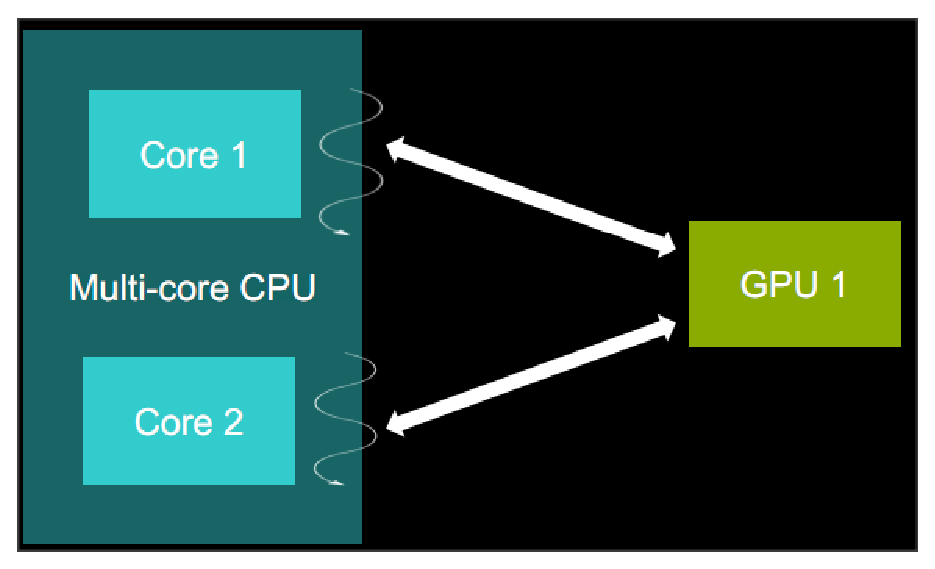
\includegraphics[height=5cm,angle=0]{./images/ABC.eps}}
\caption{Multiple host threads share a single GPU}
%\label{fig:ABC}
\label{fig:hostthread-GPU2}
\end{figure}

\begin{figure}[hbt]
   \centerline{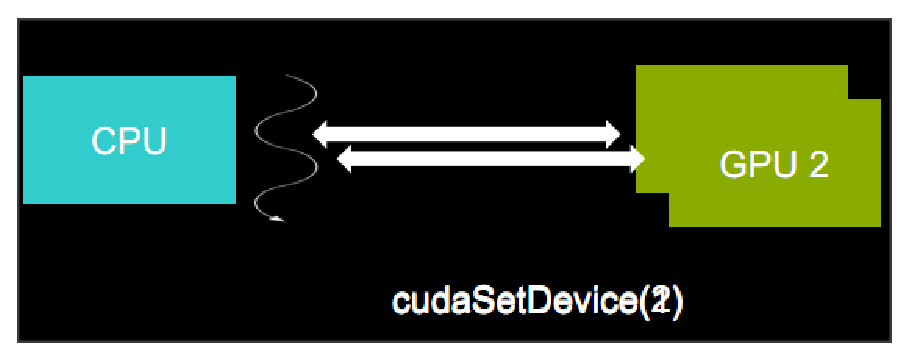
\includegraphics[height=5cm,angle=0]{./images/CDF.eps}}
% \centerline{\includegraphics[height=5cm,angle=0]{./images/singlehosthread_multipleGPU2.eps}}  
%   \centerline{\includegraphics[height=5cm,
%     angle=0]{./images/singlethreadGPU.eps}} 
\caption{Single host thread can switch between GPUs using
cudaDeviceSet(dev\_ID)}
\label{fig:hostthread_multipleGPU2}
\end{figure}


\begin{framed}
UVA, GPUDirect and 3D grids are only supported in Fermi-based GPU cards. Maximum
numbers of GPUs of UVA and GPUDirect is 9.

UVA allows kernel to get access to CPU data directly; but not in the opposite
way. Aslo, one device cannot get access to other device memory, unless using
Tesla T20 with GPUDirect 2.0.

GPUDirect cannot be used through OpenCL.

GPUDirect 2.0 cannot be used with GTX 460; but it works with GTX 480 and Quadro
6000.

Atomic operations are supported only within a GPU, not across GPUs.

UVA works on Gefore 4xx and 5xx.
\end{framed}

\subsubsection{Layered texture}
\label{sec:layered_texture}

A layered texture consists of several textures that are partially transparent
and are laid one on top of the other to create a more complex texture. 

You create layered textures by listing two or more textures one right after the
other. The last texture listed will be the top layer, the first one listed will
be the bottom layer. All textures in a layered texture other than the bottom
layer should have some transparency. For
example\footnote{\url{http://www.povray.org/documentation/view/3.6.1/356/}}:
\begin{lstlisting}
 object {
    My_Object
    texture {T1}  // the bottom layer
    texture {T2}  // a semi-transparent layer
    texture {T3}  // the top semi-transparent layer
  }
\end{lstlisting}

 CUDA 4.0 supports layered textures with large size 16K x 16K x 2K, which is
 good for medical imaging and terrain rendering (flight simulator). Using
 layered texture, there is no need to create/manage a texture alias, also it 
 \begin{itemize}
   \item interop with OpenGL/Direct3D for each layer faster
   \item has more efficient filter caching, making it runs faster than 3D
   textures
   \item reduce CPU overhead, by single binding for entire texture array.
   \item use linear/bilinear filtering applied only within a layer, so it's has
   no sampling artifacts
 \end{itemize}

 

\subsection{CUDA 4.1}
\label{sec:CUDA_41}


With CUDA 4.1, GPUDirect programming is made easier without any kernel patch
nor environment variable setting. We just install OFED and it will work, i.e.
new allocation path is enabled by default.

A major change in CUDA 4.1 is LLVM-based CUDA compiler, 1000+ new image
processing functions (with over 2000 functions in Nvidia Primitive Performance
(NPP) library) and redesign of Visual Profiler (automated performance analysis +
integrated expert guidance). LLVM-based CUDA compiler enhances +10\% performance
for many applications. 

There are some concern about the difference in double precision between CUDA 4.0
and
4.1\footnote{\url{http://forums.developer.Nvidia.com/devforum/discussion/2016/cuda-4.0-vs-cuda-4.1-same-code-different-results}}

A compiler is a development toolchain that serve as source-code building,
debugging, and deployment. There is a number of phases:
\begin{enumerate}
  \item Front-end Parser: perform initial language-specific syntax and semantic
  analysis. If the code passes this stage, then
  \item Optimizer: optimize the code, e.g. removing redundancies or dead code\ldots
  \item Code Geenrator: take the optimized code, and map to assembly code
  (not human readable)
  \item Assembler: convert assembly code to machine-code (binary code and is
  machine-dependent)
  \item Linker: if you have multiple object files, this link them into a single
  executable file.
\end{enumerate}
LLVM (Low-level Virtual Machine) is a compiler
infrastructure (written in C++) started in 2000 at UIUC and released in 2003
that revise the above phases. It emphasizes Just-in-Time compilation, cross-file optimization
(cross-language code can be linked), and modular design that allows adding more
components to the compiler tools
easily\footnote{\url{http://www.appleinsider.com/articles/08/06/20/apples_other_open_secret_the_llvm_complier.html}}.

With the advances in multi-core technology, LLVM-based compiler is hoped to make
parallel code development better. CUDA LLVM-based compiler then can target CUDA
code to other platform, e.g. new CPU technology, and support new language easily
(other than C, C++, Fortran\ldots).

CUDA 4.1 supports cuRAND (Sect.\ref{sec:cuRAND_CUDA4.1}) with 
\begin{enumerate}
  \item pseudo- and quasi-RNG (multi-dimension)
  \item several output distributions
  \item new RNGs: MRG32k3a RNG
  \item new RNGs: MTGP11213 Mersenne Twister RNG
\end{enumerate}

References:
\begin{enumerate}
  \item \url{http://llvm.org/}
\end{enumerate}
\subsection{CUDA 4.2}
\label{sec:CUDA_42}

CUDA 4.2 starts to support Kepler architecture, the third generation of
CUDA-capable GPUs from Nvidia. 

\subsection{CUDA 5.0}
\label{sec:CUDA_50}

support CC 3.5  and Dynamic Parallelism


no C++11 features are available in CUDA 5.0 RC. nvcc still does not understand C++11 syntax 

the most recent supported GCC is 4.6 for certain distributions (and older for other distributions).
 
\url{https://developer.nvidia.com/cuda-toolkit-50-archive}

\url{http://on-demand.gputechconf.com/gtc/2012/presentations/SS104-CUDA-5-What's-New.pdf}

\subsection{CUDA 5.5}
\label{sec:CUDA_55}

The CUDA SDK is part of the CUDA Toolkit package from CUDA 5.5.

\subsection{CUDA 6.0}
\label{sec:CUDA_60}

CUDA 6.0 does not support the C++11 standard,
\url{https://stackoverflow.com/questions/25941117/c11-standard-with-cuda-6-0}

CUDA 6.0 introduces the TRUE unified virtual addressing space (UVA), compared to
that introduced since CUDA 4.0 (Sect.\ref{sec:cuda4_UVA}).

The data must be allocated using \verb!cudaMallocManaged!
(Sect.\ref{sec:cudaMallocManaged}), and freed using \verb!cudaFree()!.

This requires CUDA-capable devices with compute capability $\ge$ 3.0 (preferably
5.x), running 64-bit Linux.


\subsection{CUDA 7.0 (2015)}
\label{sec:CUDA-7.0}

This is the first CUDA version to support C++11.


\subsection{CUDA 7.5}
\label{sec:CUDA_75}

\subsection{CUDA 8.0 (2016)}
\label{sec:CUDA_80}

CUDA 8.0 works with Ubuntu 16.04.
CUDA Toolkit 8 RC with support for Pascal based GeForce GTX 1080.
(Chap.\ref{chap:Pascal-GPU}).

\begin{enumerate}
  \item expecting GCC5.4 (or prior).
  
  May support GCC6 if you hack the code check
  
  \item support Pascal GPU (Sect.\ref{sec:Pascal-GPU})
\end{enumerate}

\subsection{CUDA 9.0 (2017)}
\label{sec:CUDA_90}

CUDA 9.0 works with x86-64 (Ubuntu 16.04 and 17.04) and ppc64le (Ubuntu 16.04).
\begin{enumerate}
  \item faster, reducing compile time on average by 20\% and up to 50\% compared to CUDA 8.
  
  
  \item first to support Volta GPU (Sect.\ref{sec:GPU-Volta}).
  
  \item a preview API for programming Tesla V100 Tensor Cores
  
  \item new Cooperative Groups programming model called {\bf Cooperative Groups}
  (Sect.\ref{sec:Cooperative-Group})
  
  \item nvcc compiler adds support for C++14
  
includes new features such as
\begin{itemize}
  
  \item  Generic lambda expressions inside CUDA kernel, where the auto keyword
  is used in place of parameter types
  
\begin{verbatim}
auto lambda = [](auto a, auto b) { return a * b; };
\end{verbatim}


  \item return type reduction: using the auto keyword for the return type
  
  \item fewer restrictions on what can be included in constexpr functions,
  including variable declarations, if, switch, and looping.

\end{itemize}  
\end{enumerate}


\begin{verbatim}
Windows platform:

	%ProgramFiles%\NVIDIA GPU Computing Toolkit\CUDA\v#.#

Linux platform:

	/usr/local/cuda-#.#

Mac platform:

	/Developer/NVIDIA/CUDA-#.#

\end{verbatim}


100+ CUDA examples:
\begin{verbatim}
Windows platform:
	%ProgramData%\NVIDIA Corporation\CUDA Samples\v#.#

Linux platform:
	/usr/local/cuda-#.#/samples

and
	$HOME/NVIDIA_CUDA-#.#_Samples

Mac platform:
	/Developer/NVIDIA/CUDA-#.#/samples
\end{verbatim}

NVIDIA Nsight Visual Studio Edition (Windows only)
\begin{verbatim}
Description

NVIDIA Nsight Development Platform, Visual Studio Edition is a
development environment integrated into Microsoft Visual
Studio that provides tools for debugging, profiling, analyzing
and optimizing your GPU computing and graphics applications.


Default Install Location of Nsight Visual Studio Edition

Windows platform:
	%ProgramFiles(x86)%\NVIDIA Corporation\Nsight Visual Studio Edition #.#
\end{verbatim}

\begin{verbatim}
Component : CUDA Runtime
  Windows : cudart.dll, cudart_static.lib, cudadevrt.lib
  Mac OSX : libcudart.dylib, libcudart_static.a, libcudadevrt.a
  Linux   : libcudart.so, libcudart_static.a, libcudadevrt.a
  Android : libcudart.so, libcudart_static.a, libcudadevrt.a

Component : CUDA FFT Library
  Windows : cufft.dll, cufftw.dll, cufft.lib, cufftw.lib
  Mac OSX : libcufft.dylib, libcufft_static.a, libcufftw.dylib, libcufftw_static.a
  Linux   : libcufft.so, libcufft_static.a, libcufftw.so, libcufftw_static.a
  Android : libcufft.so, libcufft_static.a, libcufftw.so, libcufftw_static.a

Component : CUDA BLAS Library
  Windows : cublas.dll, cublas_device.lib
  Mac OSX : libcublas.dylib, libcublas_static.a, libcublas_device.a
  Linux   : libcublas.so, libcublas_static.a, libcublas_device.a
  Android : libcublas.so, libcublas_static.a, libcublas_device.a

Component : NVIDIA "Drop-in" BLAS Library
  Windows : nvblas.dll
  Mac OSX : libnvblas.dylib
  Linux   : libnvblas.so

Component : CUDA Sparse Matrix Library
  Windows : cusparse.dll, cusparse.lib
  Mac OSX : libcusparse.dylib, libcusparse_static.a
  Linux   : libcusparse.so, libcusparse_static.a
  Android : libcusparse.so, libcusparse_static.a

Component : CUDA Linear Solver Library
  Windows : cusolver.dll, cusolver.lib
  Mac OSX : libcusolver.dylib, libcusolver_static.a
  Linux   : libcusolver.so, libcusolver_static.a
  Android : libcusolver.so, libcusolver_static.a

Component : CUDA Random Number Generation Library
  Windows : curand.dll, curand.lib
  Mac OSX : libcurand.dylib, libcurand_static.a
  Linux   : libcurand.so, libcurand_static.a
  Android : libcurand.so, libcurand_static.a

Component : CUDA Accelerated Graph Library
  Windows : nvgraph.dll, nvgraph.lib
  Mac OSX : libnvgraph.dylib, libnvgraph_static.a
  Linux   : libnvgraph.so, libnvgraph_static.a
  Android : libnvgraph.so, libnvgraph_static.a
\end{verbatim}

\subsection{CUDA 9.1}
\label{sec:CUDA_9.1}

\url{http://blog.exxactcorp.com/nvidia-issues-cuda-9-1-update/}

CUDA 9.1 brings new algorithms and optimizations that speed up AI and HPC apps on Volta GPUs.
\begin{enumerate}
  
  \item   develop  image augmentation algorithms for deep learning easily with
  new functions in NVIDIA Performance Primitives
  
  
  \item Run batched neural machine translations and sequence modeling operations
  on Volta Tensor cores using new APIs in cuBLAS
  
  \item Solve large 2D and 3D FFT problems more efficiently on multi-GPU systems
  with new heuristics in cuFFT
  
  \item Launch kernels up to 12x faster with new core optimizations
\end{enumerate}
\url{https://docs.nvidia.com/cuda/cuda-toolkit-release-notes/index.html#major-components}

\subsection{CUDA 9.2}
\label{sec:CUDA_9.2}

CUDA 9.2
\begin{enumerate}
  \item GCC gcc-7.3.1 support
  
\begin{verbatim}
/usr/local/cuda/bin/..//include/crt/host_config.h:119:2: error: #error 
	-- unsupported GNU version! gcc versions later than 6 are not supported!
	
	
Fixed by modifying ../include/crt/host_config.h:119 in your case from >6 to >8.
\end{verbatim}

  
  \item support VS 2017 Update 6
  
  \item requires CUDA driver 396.26+
  
\begin{verbatim}
nvidia-smi


\end{verbatim}
  
  \item CUB 1.7.5 has been integrated as a device back end for Thrust
  
  \item officially works on Ubuntu 16.04:

  However, we can also install CUDA 9.2 on Ubuntu 18.04.
  
  \url{https://www.pugetsystems.com/labs/hpc/How-to-install-CUDA-9-2-on-Ubuntu-18-04-1184/}
\end{enumerate}

\url{https://bugs.funtoo.org/browse/FL-5175}

CUDA 9 environment
\begin{verbatim}
export PATH=$PATH:/usr/local/cuda-9.2/bin
export CUDADIR=/usr/local/cuda-9.2
export LD_LIBRARY_PATH=$LD_LIBRARY_PATH:/usr/local/cuda-9.2/lib64
\end{verbatim}

Build CUDA 9.2 samples
\begin{verbatim}
source ~/misc/cuda9.2-env
// or using module
module load cuda/9.2

---------
cd ~//usr/local/cuda-9.2/samples
make -j4
\end{verbatim}

\url{https://askubuntu.com/questions/1077061/how-do-i-install-nvidia-and-cuda-drivers-into-ubuntu}

\subsection{CUDA 10.0 (2018)}
\label{sec:CUDA_10.0}

CUDA 10.0 
\begin{enumerate}
  \item supports the new Turing GPU architecture (Sect.\ref{sec:GPU-Turing}).

CUDA 10.0 is bundled with the new 410.x display driver for Linux which will be
needed for the 20xx Turing GPU's.

  \item first CUDA release with official support for Ubuntu 18.04. 
  
 This CUDA version has full support for Ubuntu 18.4 as well as 16.04 and 14.04. 
  
  \item new task-graph programming model (Sect.\ref{sec:task-graph-programming-model})
  
  \item new Nsight product family of tools for tracing, profiling, and debugging of CUDA applications
  
  
\end{enumerate}



NVIDIA driver 410.x is currently in beta version; and the ppa's package is not yet ready, i.e.
a "raw" install of the driver from NVIDIA's base package is need to use CUDA 10.0.
 
CUDA 10.0 environment
\begin{verbatim}
export PATH=$PATH:/usr/local/cuda-10.0/bin
export CUDADIR=/usr/local/cuda-10.0
export LD_LIBRARY_PATH=$LD_LIBRARY_PATH:/usr/local/cuda-10.0/lib64
\end{verbatim}


Build CUDA 10.0 samples
\begin{verbatim}
source ~/misc/cuda10.0-env
// or using module
module load cuda/10.0

---------
cd ~//usr/local/cuda-10.0/samples
make -j4
\end{verbatim}

\url{https://www.pugetsystems.com/labs/hpc/How-To-Install-CUDA-10-together-with-9-2-on-Ubuntu-18-04-with-support-for-NVIDIA-20XX-Turing-GPUs-1236/}
 
\url{https://askubuntu.com/questions/1077061/how-do-i-install-nvidia-and-cuda-drivers-into-ubuntu}

\subsection{supporting library}

\begin{verbatim}
sudo apt-get install freeglut3-dev build-essential libx11-dev libxmu-dev libxi-dev libgl1-mesa-glx libglu1-mesa libglu1-mesa-dev libglfw3-dev libgles2-mesa-dev

\end{verbatim}


\section{CUDA on Windows}
\label{sec:cuda-windows}


One big pain with CUDA under Windows Vista or Seven is that performances suffers
a lot from limits and overheads imposed by the WDDM (Windows Display Driver
Model) the driver has to comply to.
\url{http://blog.icare3d.org/2010/04/tesla-compute-drivers.html}
\begin{itemize}
  \item kernel launch overhead is $\sim 3\mus$ on non-WDDM platforms; and $\sim 40 \mus$
  at minimum and can potentially be much larger.
  
  \item
\end{itemize}
The TCC driver is a special non-graphics driver offered only on Windows
platforms as an alternative to the standard WDDM graphics driver which incurs a
lot of overhead due to deep interference of the OS with GPU operation. As you
noticed, the TCC driver is not supported with all GPUs.

{\bf IMPORTANT}: {\bf Titan GPU} does not support TTC. "NVIDIA GeForce GPUs do not support TCC mode"
The only reason to pick a K20Xm over Titan is if you need TCC mode/ECC memory support.

In Windows, you can run \verb!nvidia-smi! with \verb!-c! option
\begin{verbatim}
   -c,   --compute-mode=       Set MODE for compute applications:
                                0/DEFAULT, 1/EXCLUSIVE_THREAD,
                                2/PROHIBITED, 3/EXCLUSIVE_PROCESS
\end{verbatim}

NOTE: If you use WDDM mode, you may get the error
\begin{verbatim}
C:\Program Files\NVIDIA Corporation\NVSMI>nvidia-smi -i 1 -c 1
Unable to set compute mode for GPU 0000:02:00.0: WDDM devices may only run in DEFAULT compute mode
Treating as warning and moving on.
\end{verbatim}
You may need to also enable \verb!-dm=1!
\begin{verbatim}
   -dm,  --driver-model=       Enable or disable TCC mode: 0/WDDM, 1/TCC
\end{verbatim}


\subsection{Drivers}
\label{sec:drivers}

\url{http://www.nvidia.com/Download/index5.aspx?lang=en-us}
\begin{itemize}
\item Vista (32/64)
\item Windows 7 (32/64)
\item Window Server (use with S1070, S
\end{itemize}

Quadro (NVIDIA 196.28) for Window Server: \url{http://www.nvidia.com/content/DriverDownload-March2009/confirmation.php?url=/Windows/Quadro_Certified/196.28/196.28_Tesla_winserver2008R2_64bit_international_whql.exe&lang=us&type=Quadro}

If the CUDA-capable device is being used for display, then the maximum runtime
for the kernel is 5
(s)\footnote{\url{http://stackoverflow.com/questions/497685/how-do-you-get-around-the-maximum-cuda-run-time}}.
This is because watchdog timer that kills any shader program that run too long. This is to prevent bug in calculation on GPU for long time run. You should split the kernel into separate smaller one which take less
time to run. Otherwise, you can disabled watchdog timer in Windows, but it's
highly NOT recommended. What you can do is either
\begin{enumerate}
  \item Adjust the time (Windows XP SP1)
  \begin{verbatim}
  HKEY_LOCAL_MACHINE\SYSTEM\CurrentControlSet\Control\
  Watchdog\Display\BreakPointDelay
  \end{verbatim}
  
  \item Create on regedt32 (Windows XP 64)
  \begin{verbatim}
   HKEY_LOCAL_MACHINE\SYSTEM\CurrentControlSet\Control\Watchdog\Display\DisableBugCheck
  \end{verbatim}
  or (Vista or Windows 7), use
  \footnote{\url{http://msdn.microsoft.com/en-us/windows/hardware/gg487368.aspx,
  http://msdn.microsoft.com/en-us/library/ff569918.aspx}} create a
  \verb!REG_DWORD! and set it to 1.
  \item 
\end{enumerate}


\subsection{CUDA on Vista}
\label{sec:cuda-vista}


\section{GPU status (compute mode)}
\label{sec:gpu-status}

A Tesla GPU card may stay in one of the three states below
\begin{itemize}
\item default compute mode: it allow multiple host subprogram can get
  access to the device
\item exclusive compute mode: only one host subprogram can use the
  device at a time
\item prohibited compute mode: no host subprogram can use the device
\end{itemize}
We can check the state of the device using
\begin{enumerate}
\item \verb.cudaGetDeviceProperties(computeMode=prob, devnum).: with
  prob of type {\it type(cudadeviceprop)} and devnum is the device ID.
\end{enumerate}

You can also choose a device satisfying a given property using
\verb.cudaChooseDevice(devnum, prop). which return the device ID,
devnum, that best match the properties given in prop
\begin{lstlisting}
integer cudaChooseDevice(devnum, prop)
  integer, intent(out) :: devnum
  type(cudadeviceprop), intent(in) :: prop
\end{lstlisting}
\url{http://developer.download.nvidia.com/compute/cuda/4_1/rel/toolkit/docs/online/group__CUDART__TYPES_g7eb25f5413a962faad0956d92bae10d0.html}



%%% Local Variables: 
%%% mode: latex
%%% TeX-master: "gpucomputing"
%%% End: 
\section{Compiling tools}
\label{sec:compile-tools-CUDA}
\label{sec:cuda-compilation-howto}

This section, we study how the tools work in concert to compile the CUDA source
file. A CUDA source file (\verb!.cu! extension) is a mixture of C/C++ `host'
code and GPU `device' function\footnote{The host code is the code to run on CPU,
while the device code is the one to run on GPU.}.

The compilation phases is discussed in Sect.\ref{sec:compilation-phases} and
should be read in parallel with this section.
  
\subsection{CUDA file (.cu extension; or -x cu option)}
\label{sec:CUDA-file-definition}

A CUDA file is a file that contains CUDA code (Sect.\ref{sec:cuda-code}).

NVCC (Sect.\ref{sec:nvcc}) consider a file as a CUDA file  if either the file
ending with \verb!.cu!, or when NVCC compiling any file with the command line
option \verb!-x cu!.
Check also \verb!__CUDAC__! macro (Sect.\ref{sec:__CUDACC__-macro}).

By default, nvcc recognizes the extensions
\begin{verbatim}
.cu         --> CUDA host + device code
.c          --> C code
.cc         --> C++ code

You can enforce the file to a particular type by passing the option to nvcc

-x c
-x c++
-x cu
\end{verbatim}

\subsection{clang (CUDA)}
\label{sec:clang-cuda}

\url{https://llvm.org/docs/CompileCudaWithLLVM.html}


Clang detects that you’re compiling CUDA code by noticing that your filename
ends with .cu. Alternatively, you can pass -x cuda

\begin{verbatim}
clang++ axpy.cu -o axpy --cuda-gpu-arch=<GPU arch> \
    -L<CUDA install path>/<lib64 or lib>             \
    -lcudart_static -ldl -lrt -pthread
\end{verbatim}

Although clang’s CUDA implementation is largely compatible with NVCC’s, you may
still want to detect when you’re compiling CUDA code specifically with clang.

When clang is actually compiling CUDA code – rather than being used as a subtool
of NVCC’s – it defines the \verb!__CUDA__! macro.

NOTE: Both clang and nvcc define \verb!__CUDACC__! during CUDA compilation.

\begin{lstlisting}

#if defined(__clang__) && defined(__CUDA__) && !defined(__CUDA_ARCH__)
// clang compiling CUDA code, host mode.
#endif

#if defined(__clang__) && defined(__CUDA__) && defined(__CUDA_ARCH__)
// clang compiling CUDA code, device mode.
#endif

\end{lstlisting}

\subsection{nvcc (andd gcc version to use)}
\label{sec:nvcc}

\verb!nvcc! is the tool you need to compile a CUDA file (Sect.\ref{sec:CUDA-file-definition}).
However, you can also use it to compile a regular C/C++ file.

\textcolor{red}{Another way to compile .cu file is using clang} (Sect.\ref{sec:clang-cuda})

nvcc automatically includes CUDA-specific header files (and thus some CUDA-specific macros)
\begin{verbatim}
//nvcc automatically include

#include <cuda_runtime.h>
\end{verbatim}
when handling CUDA file.

\begin{mdframed}

IMPORTANT: \textcolor{red}{nvcc is not a compiler; instead, it is a {\bf
compiler driver}}.  So, it can be used to compile existing C host code as well,
and this relies on \verb!gcc! (or \verb!g++!).

Depending upon CUDA version (Sect.\ref{sec:cuda-toolkit}), \verb!nvcc! may
requires a specific version of gcc. The gcc compiler is required for development CUDA app
using the CUDA Toolkit. It is not required for running CUDA applications

\begin{verbatim}
CUDA 4.1 release, gcc 4.5 is now supported. gcc 4.6 and 4.7 are unsupported.
CUDA 5.0 release, gcc 4.6 is now supported. gcc 4.7 is unsupported.
CUDA 6.0 release, gcc 4.7 is now supported.
CUDA 7.0 release, gcc 4.8 is fully supported, with 4.9 support on Ubuntu 14.04 and Fedora 21.
CUDA 7.5 release, gcc 4.8 is fully supported, with 4.9 support on Ubuntu 14.04 and Fedora 21.
CUDA 8 release, gcc 5.3 is fully supported on Ubuntu 16.06 and Fedora 23.
CUDA 9 release, gcc 6 is fully supported on Ubuntu 16.04, Ubuntu 17.04 and Fedora 25.
CUDA 9.2 release, adds support for gcc 7
There is presently (as of CUDA 9) no gcc 8 support in CUDA.
\end{verbatim}

The reason is this limitation is defined in 
\begin{verbatim}
// /usr/local/cuda/include/host_config.h
//#if __GNUC__ > 4 || (__GNUC__ == 4 && __GNUC_MINOR__ > 4)
#if __GNUC__ > 4 || (__GNUC__ == 4 && __GNUC_MINOR__ > 6)
\end{verbatim}

\textcolor{red}{CHANGE DEFAULT BEHAVIOR}:
We can tell nvcc to use what specific gcc or g++ by passing the 
option  (Sect.\ref{sec:nvcc-gcc}).

\end{mdframed}

\textcolor{blue}{Example}:
\begin{verbatim}
//hello_world.cu
int main(void){

  printf("Hello World!\n");
  return 0;
}
\end{verbatim}
Using
\begin{verbatim}
>> nvcc hello_world.cu

>> ./a.out
\end{verbatim}


\begin{figure}[hbt] \centerline{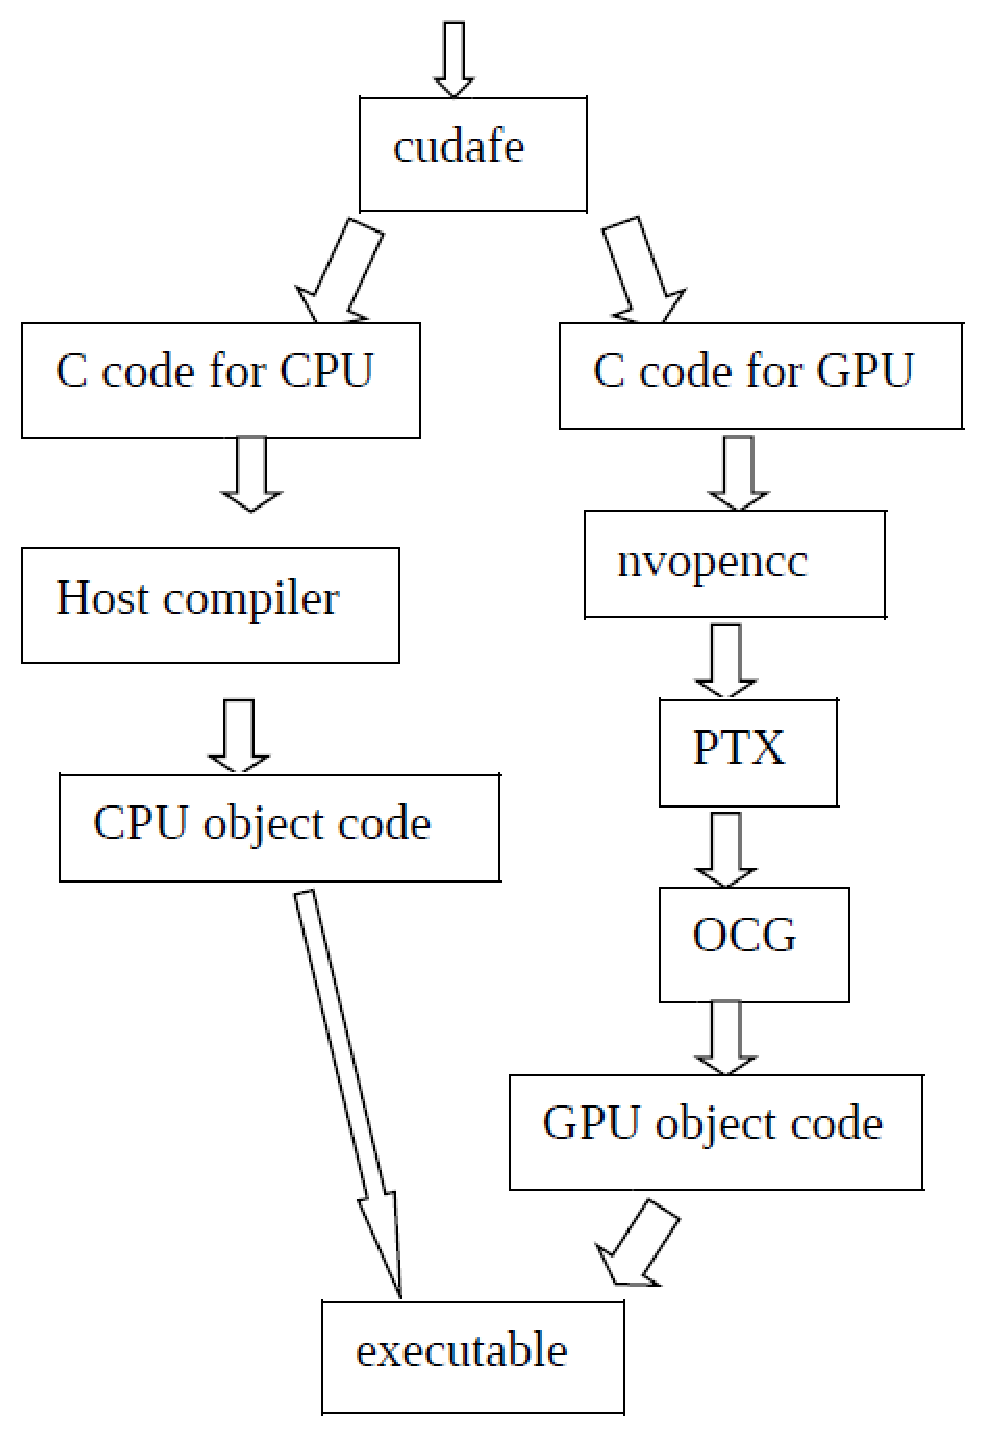
\includegraphics[height=8.5cm,
    angle=0]{./images/nvcc_toolchain.eps}}
\caption{NVCC toolchain}
\label{fig:nvcc-tool}
\end{figure}

\begin{enumerate}
  \item Step 1:

When a file is passed to \verb!nvcc! for compilation, nvcc first calls a tool to
do pre-processing for the macros and then split CUDA code and host code from
file (Sect.\ref{sec:cudafe}).
  
  \item Step 2: once the codes are separated, nvcc it will evoke the right tool
  to compile host code and GPU code, respectively.

The host code is taken cared by the host C++ compiler
(Sect.\ref{sec:host-code-compiler}).

In essence, the compilation for device functions is divided into two stages:
(1) to PTX format (Sect.\ref{sec:ptx-language}), (2) (from PTX) to cubin format
by ptxas (Sect.\ref{sec:ptxas}), as shown in Fig.~\ref{fig:nvcc_stg}.
\begin{enumerate}
  
  \item  {\bf Stage 1:} The device code (extracted and saved in file with extension
\verb!.gpu!) will be compiled by the proprietary NVIDIA C/C++
compiler/assembler, called {\bf nvopencc} (Sect.\ref{sec:nvopencc}) into
Nvidia's virtual assembly PTX.

The output of \verb!nvopencc! are intermediate files whose content are the codes
written in an intermediate language called {\bf PTX} ({\it parallel thread
execution})\footnote{PTX programs are always in text format} (.ptx) (Read
Sect.~\ref{sec:ptx-language}).  The compilation can stop here, as the PTX code
can be invoked by the program for {\it just-in-time compilation} and run on any
CUDA-capable device that support this version of PTX. However, to interpret
these PTX files, we still need the two libraries cudart.so and cuda.so
(Sect.\ref{sec:gener-intermd-files}).

  \item {\bf Stage 2:}: Next, the PTX code is compiled into the
binary format (.cubin) that can be executed by the GPU by a well-tuned low-level
compiler (ptxas). \verb!.cubin! file contains optimized GPU binary code (or GPU
object code).

The compilation of PTX file into generate  (\verb!.cubin!) via first an {\bf
OCG}  (Optimized Code Generator) called {\bf ptxas}, a well-tuned low-level 
compiler for graphics code. 
 
  \item {\bf Stage 3:} To create an x86 executable file, in the end, the GPU
  object code can be embeded
into the CPU object code to create the binary program using the tool
\verb!fatbin! (Sect.\ref{sec:fatbin}). The binary file can be embedded with the
PTX and/or the CUBIN targetted to one or more versions of GPU.

  
  Then, \verb!nvcc! will call {\bf fatbin} (fat binary) to embed the GPU object
  code (.cubin) into the CPU object code (.o, .obj) to create the executable
  file or  library (.out, .exe). This code is hardware-specific; and thus can
  only be run on CUDA-capable device with a specific compute capability only
  (Sect.\ref{sec:compute-capability}).
 
Without the PTX code embedded, the CUDA binary program can only run on the GPU
architecture that CUBIN was designed to run on. The detail of all stages is
mentioned in Sect.\ref{sec:compilation-phases}.
  
\end{enumerate}

The stages for building CUDA code is given in Fig.~\ref{fig:nvcc-tool}. The
outputs at intermediate stages will be deleted by default. However, we can ask
to keep them for further investigation if needed
(Sect.\ref{sec:gener-intermd-files}).


\end{enumerate}



% The GPU functions will be compiled by NVIDIA  Open64
% compiler\footnote{\url{http://en.wikipedia.org/wiki/Open64}}, called {\bf
% nvopencc}.
\begin{figure}[hbt]
  \centerline{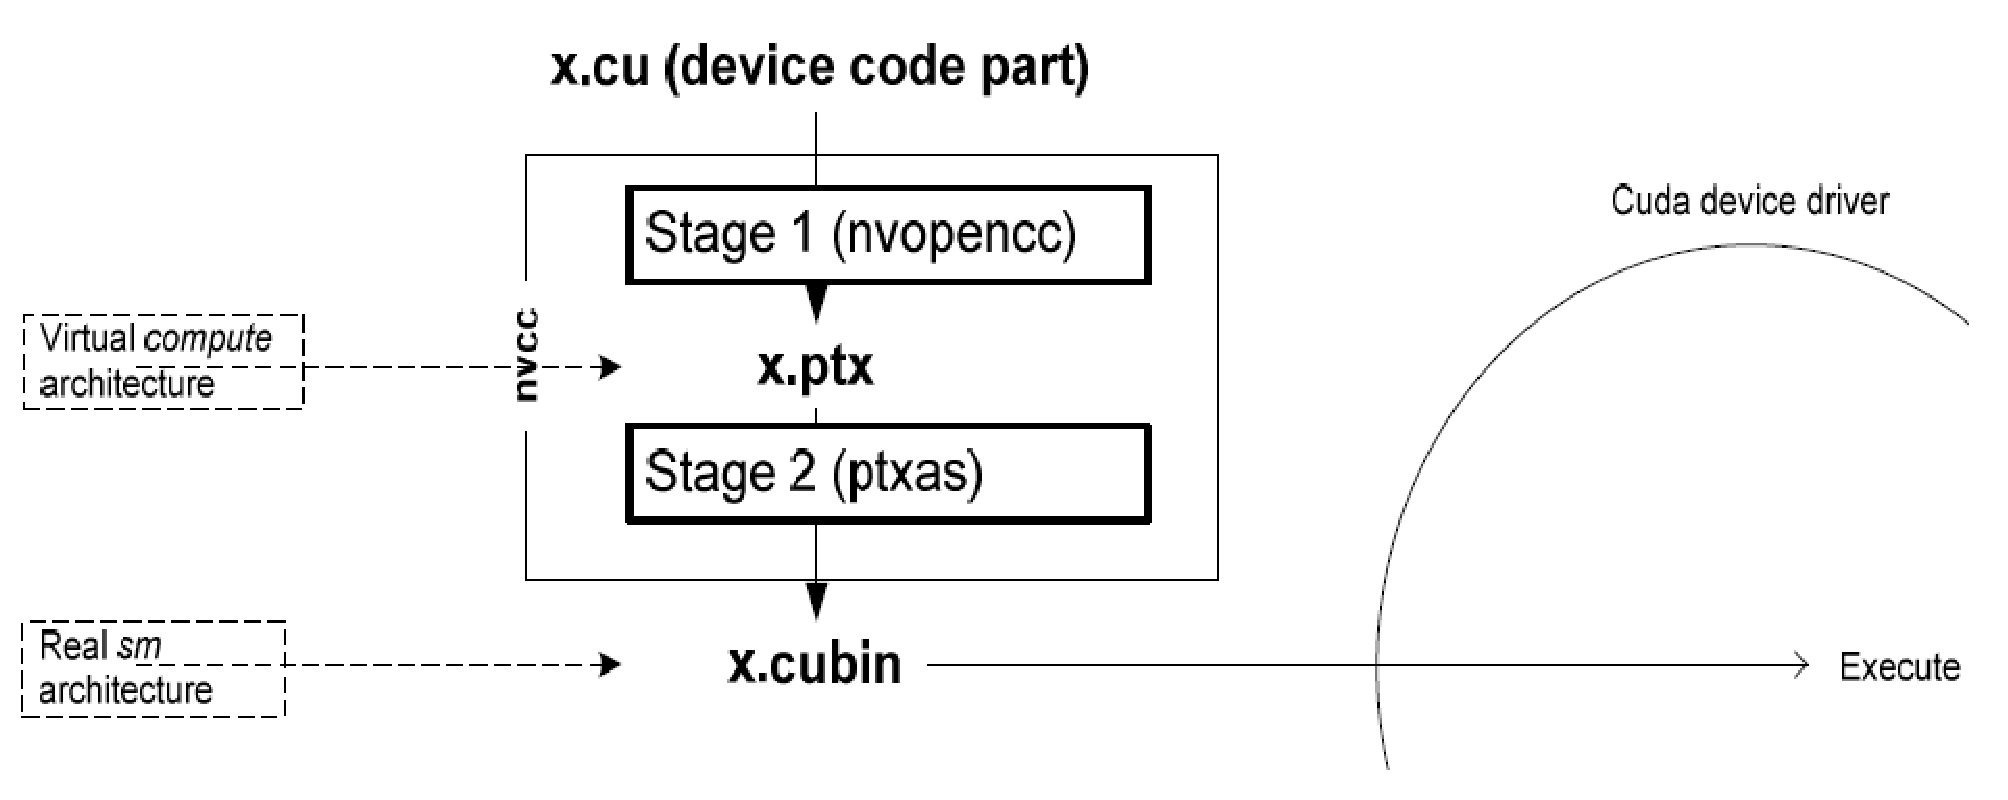
\includegraphics[height=5cm,
    angle=0]{./images/nvcc_compile.eps}}
\caption{NVCC 2 stages}
\label{fig:nvcc_stg}
\end{figure}


\subsection{-- choose gcc/g++ version to work with nvcc}
\label{sec:nvcc-gcc}
\label{sec:host-code-compiler}
 
 
\begin{itemize}
\item In Linux: \verb!gcc! (for C language), \verb!g++! (for C++ language)
\item In Window: Microsoft Visual Studio (\verb!cl!); use of
  \verb!gcc! or \verb!mingw32-g++! is not supported.
\end{itemize}

\textcolor{red}{CHANGE DEFAULT BEHAVIOR}:
We can tell nvcc to use what specific gcc or g++ by passing the 
option 
\begin{verbatim}
-ccbin <gcc-binary>
\end{verbatim}
to \verb!nvcc!.
To change the above default behavior, you have the option
\begin{enumerate}
  
  \item  It is possible to configure nvcc to use the correct version of gcc
  without passing any compiler parameters by adding softlinks to the bin
  directory created with the nvcc install.
\begin{verbatim}
// suppose /packages/cuda/7.5/bin/nvcc
// (default is /usr/local/cuda/bin/)


// then 
sudo ln -s /usr/bin/gcc-4.4 /packages/cuda/7.5/bin/gcc

\end{verbatim}
  \item configure the new gcc version to where CUDA toolkit search
  
\begin{verbatim}
// the newer gcc version
sudo apt install gcc-4.4

// link to 
sudo ln -s /usr/bin/gcc-4.4 /usr/local/cuda/bin/gcc

// finally install CUDA
\end{verbatim}  
\end{enumerate}

\url{https://docs.nvidia.com/cuda/cuda-installation-guide-linux/index.html#axzz3x7mwvZrG}

The host functions 
\begin{itemize}
  \item In Linux: extracted and saved in file with extension \verb!.cu.c!  
  \item In Windows: extracted and saved in file with extension \verb!.cu.pp!, \verb!.cpp<num>.i!, \verb!cpp<num>.res!
\begin{verbatim}
filename.cpp1.ii
filename.cpp1.res
filename.cpp2.i
filename.cpp2.res
filename.cu.cache
filename.cu.cpp.ii
filename.cu.cpp.ii.res
\end{verbatim}  
\end{itemize}
will be compiled by the corresponding compiler to object file (.obj, .o)
\footnote{The location of the C/C++ compiler will be assumed to be in
  the search path, unless option {\bf -compiler-bindir} is specified.
}

\subsection{cudafe}
\label{sec:cudafe}


The preprocessor \verb!cudafe! (CUDA front-end) reads the source files and convert it into
the final C source file after preprocessing all macros. 

\verb!cudafe!  is called first by \verb!nvcc!, which do (1) pre-processing, (2)
separate the device functions from the `host' codes. 

NOTE: By default, you cannot use macro with variant arguments, like
\begin{verbatim}
#define debug(...) printf (__VA_ARGS__)
\end{verbatim}

This can be enable by compiling the source file with the option
\begin{verbatim}
-Xcudafe --variadic_macros
\end{verbatim}

During the compilation, \verb!nvcc! can pass different compiling options to
cudafe. E.g. You can tell \verb!nvcc! where to look
for the files using the following flags, as shown in Table \ref{tab:searchpath}.

\begin{table}[hbt]
\begin{center}
\caption{File search paths}
\begin{tabular}{lcc} 
  \hline
  Description & long flag & short flag \\ 
  \hline\hline
  location of header files\footnote{during preprocessing or compilation} &
  \verb!--pre-include include-file,...! & \verb!-include! \\
  library for linking stage & \verb!--library library-file,...!  &
  \verb!-l! \\
  define macro   & \verb!--define-macro macrodef,...! & \verb!-D! \\ 
  (if preprocessing is in used) & & \\
  undefine macro & \verb!--undefine-macro macrodef,...! & \verb!-U! \\
  source file search path  & \verb!--include-path include-path,...! & \verb!-I!
  \\
  library file search path & \verb!--library-path library-path,...! &
  \verb!-L! \\
  where to store output file & \verb!--output-directory directory! &
  \verb!-odir! \\
  where compiler reside & \verb!--compiler-bindir directory! &
  \verb!-ccbin! \\
  \hline
\end{tabular}
\end{center}
\label{tab:searchpath}
\end{table}

For example: each kernel needs \verb!extern "C" __global__! keyword in the front.
To avoid using this long form, we define the short-form \verb!__kernel__! by
defining a macro

\begin{verbatim}
#define __kernel__ extern "C" __global__
\end{verbatim}

Now, we put this definition in a header file, and \verb!#incldue! the file into
every where we use it. To avoid typing this in every file, we can ask
\verb!nvcc! (Sect.\ref{sec:nvcc}) to automatically include the file duing cudafe
phase, using \verb!--preinclude! option.
\begin{verbatim}
nvcc -c -I"C:\NVIDIA_GPU_Computing SDK_4.0\C\common\inc"
  --cudafe-options="--preinclude vector_size_header.h" 
  -v vectorAdd.cu
\end{verbatim}


\subsection{nvopencc}
\label{sec:nvopencc}

\verb!nvopencc! is a variant of Open64 compiler\footnote{\url{http://en.wikipedia.org/wiki/Open64}}
(before CUDA 3.0, it supports C
only, not C++ nor Fortran so \verb!extern "C"! is required). It is quite robust,
yet not so complicated as it has
\begin{itemize}
\item no Inter-Procedural Analysis
\item no Loop Nest Optimization
\item no preprocessing or linking
\end{itemize}
\textcolor{red}{Since CUDA 5.0, Nvidia switched to
using LLVM-based compiler}, and thus support C++ and Fortran language.

nvopencc has 3 parts:
\begin{enumerate}
\item Front end (\verb!gfec! tool): based on gcc, produces WHIRL IR
\item Inliner (\verb!inline! tool): inlines all calls
\item Back end (\verb!be! tool): optimizes and lowers WHIRL into PTX
\end{enumerate}

The Back-end phase includes
\begin{enumerate}
\item VHO (Very High Optimizer)
  \begin{itemize}
  \item switch $\rightarrow$ if/else
  \item struct copies $\rightarrow$ field copies
  \end{itemize}
\item WOPT (Whirl OPTimizer): translates WHIRL into SSA (Static Single
  Assignment) form then back to WHIRL
\item CG (Code Generator): generate PTX codes
  \begin{itemize}
  \item expand WHIRL into PTX
  \item assign virtual registers
  \item convert 32-bit ops into 16-bit ops
  \item rematerialize GRF loads to reduce live-ranges
  \item combine contiguous load/stores into vectors
  \item emit PTX
  \item no scheduling
  \item no ``real'' register allocation
  \item relies on OCG
  \end{itemize}
\end{enumerate}
The PTX code is handled by Sect.\ref{sec:ptxas}.

References:
\begin{itemize}
\item \url{www.open64.net}
\item \url{http://wiki.open64.net/images/e/eb/Nvopencc-tutorial.ppt}
\item \url{http://blog.langly.org/2009/02/12/cuda-hacking-ptx-code/}
\end{itemize}

\subsection{ptxas}
\label{sec:ptxas}

PTXAS compile the PTX text-code (Secct.\ref{sec:ptx-language}) into
\verb!.cubin! code (Sect.\ref{sec:cubin}) and create the fat binary file
(Sect.\ref{sec:fatbin}).

\subsection{filehash.exe}

CUDA 6.5

\subsection{cicc.exe}

CUDA 6.5

\subsection{cudafe++.exe}

CUDA 6.5

\subsection{fatbinary.exe (binary code .cubin)}
\label{sec:fatbin}
\label{sec:cubin}

A fat binary is a file containing both host code and device code. 

A \verb!.cubin! file contains the cubin code which is GPU-hardware specific.
To get the handle to the compiled cubin code, and to register, nvcc use 2
functions.
\begin{verbatim}
__cudaRegisterFatBinary()
__cudaRegisterFunction()

void** __cudaRegisterFatBinary(void *fatCubin);

void __cudaRegisterFunction(void **fatCubinHandle, const char *hostFun, 
                   char *deviceFun,
                   const char *deviceName, int thread_limit, uint3 *tid,
                   uint3 *bid, dim3 *bDim, dim3 *gDim, int *wSize);
\end{verbatim}
Typically, programmers use these functions to extract the PTX code from one executable file
to use in another one (for emulation) or disassembly. However, they're not meant
to be called directly by user code.

Compared to CUDA 3.x, CUDA 4.0 has changed the structure of fatCubin.
\begin{enumerate}
  \item In CUDA 3.x, it's a pointer to \verb!__cudaFatCudaBinary! structure, so
  using \verb!(__cudaFatCudaBinary)*! return the information.
  \begin{verbatim}
  typedef struct __cudaFatCudaBinaryRec {
        unsigned long         magic;
        unsigned long         version;
        unsigned long         gpuInfoVersion;
        char*                    key;
        char*                    ident;
        char*                    usageMode;
        __cudaFatPtxEntry              *ptx;
        __cudaFatCubinEntry                *cubin;
        __cudaFatDebugEntry                *debug;
        void*                   debugInfo;
        unsigned int                     flags;
        __cudaFatSymbol          *exported;
        __cudaFatSymbol          *imported;
        struct __cudaFatCudaBinaryRec *dependends;
        unsigned int                     characteristic;
        __cudaFatElfEntry              *elf;
} __cudaFatCudaBinary;
  \end{verbatim}
  Each fat binary is registered once via a global constructor
  \verb!__cudaRegisterFunction()!, once for each kernel. 
 
 To extract the PTX code from the kernel, we use Ocelot code
 \verb!extractPTXKernel()! function (\ref{sec:Ocelot}). 
  
  \item In CUDA 4.x, in Ubuntu:
  \begin{verbatim}
  typedef struct __cudaFatCudaBinary2EntryRec { 
unsigned int type;
unsigned int binary;
unsigned int binarySize;
unsigned int unknown2;
unsigned int kindOffset;
unsigned int unknown3;
unsigned int unknown4;
unsigned int unknown5;
unsigned int name;
unsigned int nameSize;
unsigned long long int unknown6;
unsigned long long int unknown7;
} __cudaFatCudaBinary2Entry;
  \end{verbatim}
  \item In CUDA 4.x, in Windows:
  
  \item In CUDA 5.0 ???
\end{enumerate}


To create \verb!cubin! code for different GPU hardware architectures, we use the
compiler option \verb!-code=! or \verb!-gencode=code=! suboption whose values
can be virtual or real architecture. However, the ``code'' architecture must be
compatible with the ``arch'' architecture.
% \begin{verbatim} -code=sm_13 !or -code=compute_13 \end{verbatim}
Using this is incorrect
\begin{verbatim}
-arch=compute_13 -code=sm_10
\end{verbatim}
as the first compilation stage create PTX code that assume the availability of
double-precision support of the GPU; yet the real GPU is not, i.e. at
\verb!sm_10! only.

\begin{framed}
To write code for different device compute capability, we can use the macro
\verb!__CUDA_ARCH__! to select the appropriate code path. This macro should be
used inside device code only (kernel). It is assigned one of the three value in
the form $xy0$ (ending a literal `0') with x is the major, y is the minor
revision.

\begin{lstlisting}
#include <stdio.h>

#ifndef __CUDA_ARCH__
#warning cuda arch not defined 
#else
#warning everything is normal
#endif

__global__ void helloCUDA(const float f) 
{ 
#if __CUDA_ARCH__ >= 200
   printf("Hello thread %d, f=%f\n", threadIdx.x, f) ; 
#endif
} 

int main() 
{ 
        helloCUDA<<<1, 5>>>(1.2345f); 
        return cudaThreadExit(); 
}
\end{lstlisting}
\end{framed}

% \subsection{Mixed binary code and PTX code (-gencode arc=,code=)}
% \label{sec:gencode}
% 
% Another compiler option that is a generalization of the two previous
% ones is \verb!-gencode! option with two sub-options separated by
% comma. By using this, we can generate different pairs of (PTX, cubin). 
% \begin{verbatim}
% -gencode arch=<arch>, code=<code>
% \end{verbatim}
% is equivalent to \verb!--generate-code arch=<arch>,code=<code>!
% We can use this option repeatedly to generate code for different
% virtual architectures.
% \begin{verbatim}
% nvcc x.cu \
%     -gencode arch=compute_10,code=sm_10 \
%     -gencode arch=compute_10,code=sm_11 \
%     -gencode arch=compute_13,code=sm_13 \
%     -gencode arch=compute_13,code=sm_20
% \end{verbatim}
% or we just leave the code for JIT compilation.
% \begin{verbatim}
% nvcc x.cu \
%     -gencode arch=compute_10,code=compute_10 \
%     -gencode arch=compute_13,code=compute_13
% \end{verbatim}
% 
% For a more complex code generation, you can do like this (NOTE: due to
% technical reasons, the combined suboption must be quoted
% \begin{verbatim}
% nvcc x.cu \
%     -gencode arch=compute_10,code='sm_10,sm_11' \
%     -gencode arch=compute_13,code='sm_13,sm_20'
% \end{verbatim}
% 

% ), i.e. PTX codes are passed to , to generate an
% optimized GPU object code  % Depending on
% % the hardware design, there are also different virtual GPU
% % architectures (called {\it compute} architecture), as well as ``real''
% % GPU architectures.


\subsection{bin2c.exe}


\section{Compilation phases}
\label{sec:compilation-phases}

CUDA works by embedding device code into host objects. 
\begin{enumerate}  
  \item In whole program compilation: if the device code and host code altogether in the same compilation unit:
  
  it embeds executable device code into the host object.
  
  \item In separate compilation, we first need to generate relocatable code (host code + device code):
  
  Next, we embed relocatable device code into the host object, and run
  \verb!nvlink!, the device linker, to link all the device code together.
  
  The output of \verb!nvlink! is then linked together with all the host objects by the
  host linker to form the final executable.
  
\end{enumerate}


In Sect.\ref{sec:compile-tools-CUDA}, we only mention 2 main
compilation phases (generate PTX file and cubin object) - Sect.\ref{sec:nvcc}). 

% Indeed, there are other
% intermediate compilation phases, yet they are for debugging purpose only, not to
% use in build scripts.  For each phase, there will be an intermediate
% file for the source code are generated. By default, they will be
% automatically deleted after the compilation.  If you want to keep all
% of them, use the flag \verb!-keep!.
% \begin{verbatim}
% nvcc acos.cu -keep
% \end{verbatim}

\subsection{Generate intermediate files}
\label{sec:gener-intermd-files}

We can control which files generated during intermediate stages should be kept.
There is a set of different options to specify the compilation phases, and
\verb!-keep! is one of them.  
\begin{verbatim}
nvcc acos.cu -keep
\end{verbatim}

Table \ref{tab:stagecompilation} shows the list of all phases, following its
compilation order, as shown in Fig.~\ref{fig:nvcc_trajectory}. By default, if
there is none of the above options, \verb!nvcc! will do all the stages, remove
all the intermediate files, and create the executable file or library. Using an
appropriate flag, you can choose at which stage the compilation should stop
and/or which intermediate files to keep.


\begin{table}[hbt]
\begin{center}
\caption{Stage compilation option}
\begin{tabular}{lcc} 
  \hline
  Stage & long flag & short flag \\ 
  \hline\hline
  generate cu.c from .cu  & \verb!--cuda! & \verb!-cuda! \\
  ({\it extract host code}) & & \\
  generate .gpu from .cu\footnote{.c/.cc/.cxx/.cpp/.cu}  & &
  \verb!-gpu! \\
  ({\it extract cuda codes}) & & \\
  check macro use & \verb!-preprocess! & \verb!-E! \\
  ({\it C/C++ preprocessing}) & & \\
  compile to object file & \verb!--compile! & \verb!-c! \\
  ({\it .o, .obj from cu.c}) & & \\
  generate .ptx from  & & \verb!-ptx! \\
  (1) .cu  & & \\
  (2) .gpu intermediate files & & \\
  generate .cubin from  &  & \verb!-cubin! \\
  (1) .cu file & & \\
  (2) .gpu,  & & \\
  (3) .PTX intermediate files & & \\
  build a static library (.a) & & \verb!-lib! \\
  generate `Make' dependency\footnote{only one source
    file(.c/.cc/.cpp/.cxx/.cu), and it will create a dependency
    file that can be used to include in the Makefile} &
  \verb!--generate-dependencies! & \verb!-M! \\
  link all inputs & & \verb!-link! \\
  build the executable file\footnote{accept only one input} &
  \verb!--output-file file! & \verb!-o! \\
  build and run the program & & \verb!-run! \\
  \hline\hline
\end{tabular}
\end{center}
\label{tab:stagecompilation}
\end{table}


\begin{figure}[hbt]
  \centerline{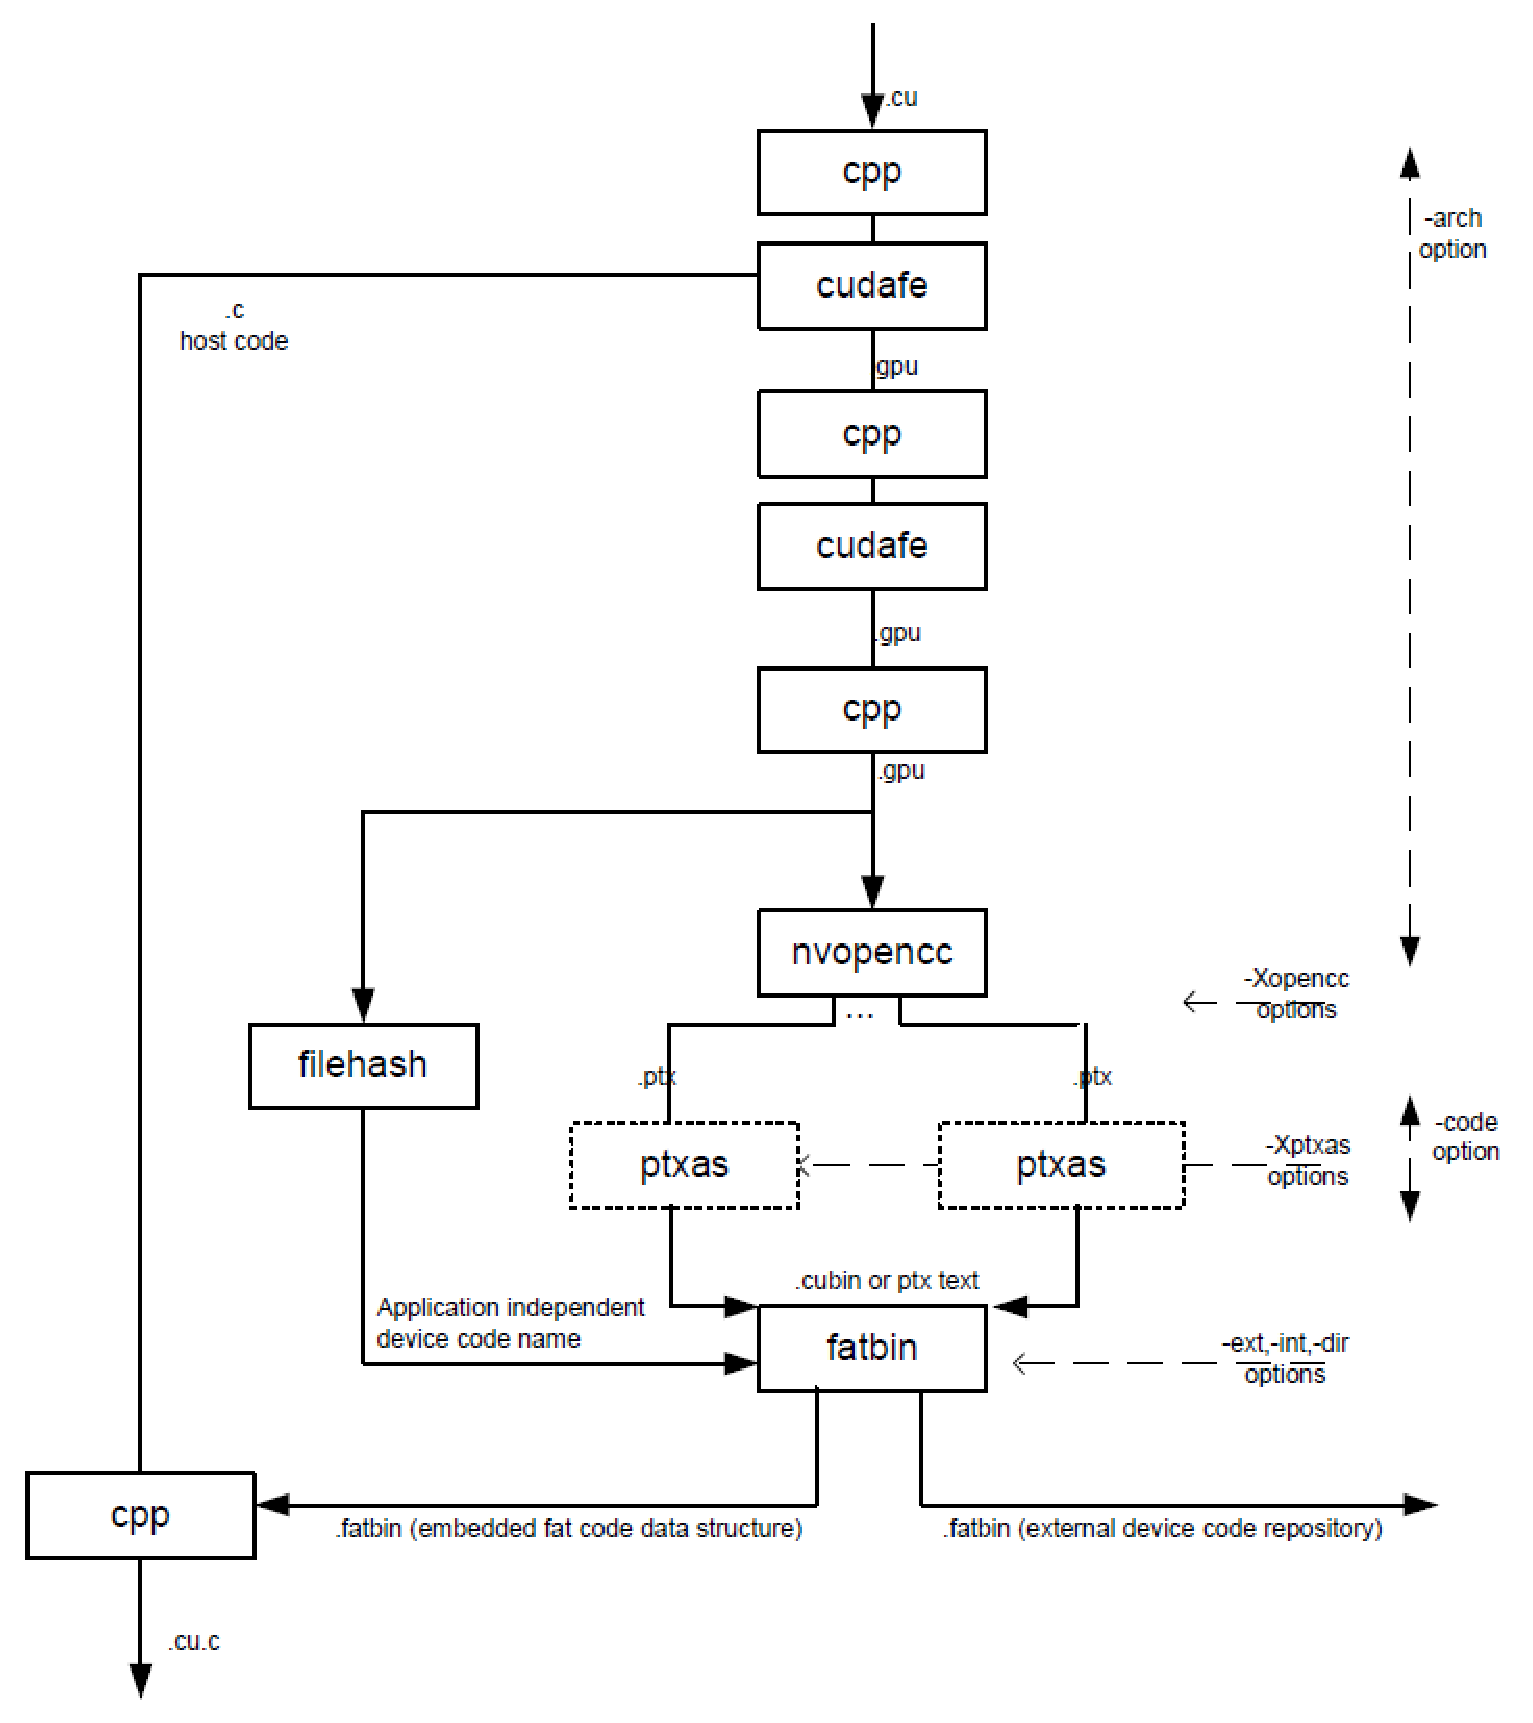
\includegraphics[height=10cm,
    angle=0]{./images/nvcc_trajectory.eps}}
  \caption{Full CUDA compilation trajectory}
\label{fig:nvcc_trajectory}
\end{figure}


For more information, type
\begin{verbatim}
nvcc --help | less
\end{verbatim}

\subsection{Clean-up intermediate files}
\label{sec:clean-up-interm}

To clean the intermediate files generated by a given compilation process
(Sect.\ref{sec:gener-intermd-files}), you need to specify the exact compiling
options you use to generate the intermediate files and then add \verb!-clean!
right to the command for that compilation process, i.e. using \verb!-clean!
alone won't do what you're expected.
\begin{verbatim}
nvcc acos.cu -keep -clean

!using this will result in a different cleanup effect
!as it only clean the intermediate files generated from 
! -c option
nvcc acos.cu -c -clean
\end{verbatim}

% \subsection{'cudafe' options}
% \label{sec:file-paths}


\subsection{Configuration file (Linux)}
\label{sec:configuration-file}

The configuration file is \verb!nvcc.profile! locate in where
\verb!nvcc! resides. Typically, it contains the minimum information
that \verb!nvcc! need to use, e.g.  the path to \verb!\bin!  (via
\verb!PATH!) and \verb!\lib! directory (via \verb!LD_LIBRARY_PATH!) of
the CUDA toolkit installation.

{\bf Example}: nvcc.profile
\begin{verbatim}
#
# nvcc and nvcc.profile are in the bin directory of the
# cuda installation tree. Hence, this installation tree
# is `one up':
#
TOP              = $(_HERE_)/..

# Extend dll search path to find cudart.so and cuda.so
# and add these two libraries to the link line
LD_LIBRARY_PATH += $(TOP)/lib:$(TOP)/extools/lib:

# Extend the executable search path to find the
# cuda internal tools:
PATH            += $(TOP)/open64/bin:$(TOP)/bin:

# Define the cuda include directories:
INCLUDES += "-I$(TOP)/include" "-I$(TOP)/include/cudart" $(_SPACE_)

LIBRARIES   =+ $(_SPACE_) "-L$(TOP)/lib$(_TARGET_SIZE_)" -lcudart

CUDAFE_FLAGS    +=
OPENCC_FLAGS    +=

# No special optimization flags for device code compilation:
PTXAS_FLAGS     +=
\end{verbatim}
In this file, except the comment lines (starting with \verb!#!), other
lines have the form: \verb!name ... <text>!, with \verb!...! can be
\begin{itemize}
\item conditionally assigned (`?=')
\item prepended (`+=')
\item appended ('=+')
\end{itemize}
To refer to the environment variable, we can use \verb!%name%!
(DOS style) or \verb!$(NAME)! ({\it make} style).

Some special macros
\begin{enumerate}
\item \verb!_SPACE_! used to force a white space in the
profile line, such as
\begin{verbatim}
INCLUDES += -I../common $(_SPACE_)
\end{verbatim}

\item \verb!_HERE_! contain the directory where \verb!nvcc.profile! is
  installed. 
\end{enumerate}


\subsection{Configuration file (Windows)}

CUDA in Windows put these configuration files in 
\begin{verbatim}
C:\Program Files (x86)\MSBuild\Microsoft.Cpp\v4.0\V120\BuildCustomizations
\end{verbatim}

with a set of 3 files for each version
\begin{verbatim}
CUDA 6.0.props
CUDA 6.0.targets
CUDA 6.0.xml

CUDA 6.5.props
CUDA 6.5.targets
CUDA 6.5.xml
\end{verbatim}

\section{Separate compilation from linking (CUDA 5.0+ and sm\_2x+ (Fermi, Kepler+))}

No Separate Compilation in earlier releases
\begin{verbatim}
main.cpp    +     (a.cu, b.cu, c.cu) ---> program.exe
\end{verbatim}
Earlier CUDA required single source file for a single kernel, and must be compiled using \verb!nvcc!.

\url{http://on-demand.gputechconf.com/gtc-express/2012/presentations/gpu-object-linking.pdf}

Since CUDA 5.0, it supports compilation stage and linking stage which can be done at two different time
\begin{verbatim}
a.cu  --> a.o
b.cu  --> b.o
c.cu  --> c.o

main.cpp + (a.o, b.o, c.o)   ----> program.exe
\end{verbatim}
Separate compilation allows building independent object files (CUDA files compiled by \verb!nvcc!, and C/C++ host code only
compiled by gcc/g++), and these objects can be linked into CUDA app via 2 steps
\begin{enumerate}
  \item nvcc to generate relocatable object files (Sect.\ref{sec:relocatable-object-file-CUDA})
  \item nvcc to link and extract CUDA code only from these object files into a separate object file, say \verb!gpuCode.o!
  \item gcc/g++ to link these object files and the \verb!gpuCode.o! together into a single executable app.
\end{enumerate}

\begin{verbatim}
a.o, b.o, c.o, d.cu  ----->  gpuCode.o   [or gpuCode.a]
	Can combine object files into static libraries

main.cpp + (a.o, b.o, c.o) + gpuCode.o ------>   program.exe
\end{verbatim}

WHY SEPARATE COMPILATION?
\begin{enumerate}
  \item   “extern” attribute is respected
  
  \item no longer have to include files together
  
  \item incremental compilation reduces build time
  
  Facilitates code reuse, reduces compile time
  
  \item can create and use 3rd party libraries.
  
  We can link static host libraries (.a,.lib) that contain device code.

  Shared libraries (.dylib,.so,.dll) are ignored by device linker.

CUDA provides \verb!libcublas_device.a! is linkable device library that we
ship and is used for dynamic parallelism (Sect.\ref{sec:dynamic-parallelism})

\end{enumerate}



\subsection{Generate relocatable CUDA code (e.g. object file)}
\label{sec:relocatable-object-file-CUDA}

The generation of relocatable vs executable device code is controlled by the --relocatable-device-code option.

Suppose we have a source file (.c/.cpp/.cu) and we want to extract the CUDA-specific code to be linked to the binary CUDA app later,
then we use one of the following option to nvcc
\begin{verbatim}
# either one is the same

--relocatable-device-code=true --compile
-dc
--device-c
\end{verbatim}

Compile each .c, .cc, .cpp, .cxx, and .cu input file into an object file that contains relocatable device code.
\begin{verbatim}
nvcc –arch=sm_20 –dc *.cu


nvcc –arch=sm_20 –dc -x cu *.cpp
\end{verbatim}
NOTE: -c is used for host compile to object, so Nividia invented \verb!-dc!.
Without –dc we default to old whole program compilation.

DEFAULT BEHAVIOR: The source file name extension is replaced by .obj on Windows
and .o on other platforms to create the default output file name.

When we run on object files
\begin{verbatim}
nvcc –arch=sm_20 *.o
\end{verbatim}
It actually run device linker.
Device linker is implicitly run for \verb!sm_20! and above, but does nothing if
does not find relocatable device code.

\subsection{-- using host linker}
\textcolor{red}{Link all object files together into a gpuCode.o object file}.

\begin{verbatim}
nvcc –arch=sm_20 *.o –dlink –o link.o


nvcc –arch=sm_20 *.o –dlink –o gpuCode.o
\end{verbatim}
create new object; -dlink == --device-link


\subsection{Generate executable CUDA app}

Current 5.0 linker will not JIT to future architectures, i.e. SASS is linked, not PTX.
PTX can be input to linker, but is first compiled to SASS then linked.

Must relink objects for each architecture
\begin{verbatim}
nvcc –arch=compute_20 –code=sm_20,sm_30
\end{verbatim}

CUDA will  support JIT linking in future release.

\subsection{-- using device linker}

CUDA host objects must be passed to both device and host linkers

The generation of relocatable vs executable device code is controlled by the --relocatable-device-code option.

\begin{verbatim}
-dw

--relocatable-device-code=false --compile.

--device-w
\end{verbatim}

Compile each .c, .cc, .cpp, .cxx, and .cu input file into an object file that contains executable device code.

DEFAULT BEHAVIOR: The source file name extension is replaced by .obj on Windows
and .o on other platforms to create the default output file name

\subsection{-- using host linker}

CUDA host objects must be passed to both device and host linkers

\begin{verbatim}
g++ *.o –lcudart
	link all objects, including new link.o (or gpuCode.o)

\end{verbatim}

\subsection{-- multiple devices link}

Can do multiple device links within a single host executable

\begin{verbatim}
nvcc a.o b.o –dlink –o link1.o

nvcc c.o d.o –dlink –o link2.o

g++ a.o b.o c.o d.o link1.o link2.o
\end{verbatim}

\section{Compiling option (-gencode)}
\label{sec:Compile_option}
\label{sec:nvcc_-gencode-option}

CUDA kernel device code is compiled to two different levels of backend target.

First read Sect.\ref{sec:nvcc} on different compilation stages from host/device C/C++ code into 
\verb!.ptx! and then \verb!.cubin! files. 
\begin{enumerate}
  \item level 1 = virtual = PTX intermediate code
  
  PTX (Portable Thread eXecution) is a forward-compatible, human-readable
  intermediate representation.
  It defines a RISC-like instruction set architecture. PTX is forward-compatible
  to all architectures, i.e. older PTX codes can be used to generate SASS code in newer GPUs.
  
  
  \item level 2 = real = hardware-specific = SASS code 
  
  SASS (Shader ASSembler) is the native, architecture-specific instruction set
  architecture for NVIDIA GPUs. It is usually generated by ptxas from PTX.
  
  SASS is only forward-compatible within the same major family (i.e., within
  Fermi, within Kepler or within Maxwell)
  
\end{enumerate}


KEEP IN MIND: Compile the CUDA code for the architecture (both virtual and real)
that represents the GPUs you wish to target. By virtual, we means generate the
PTX code, coherent to a specific version of PTX (Sect.\ref{sec:ptx-language}).

The virtual code is PTX; and the binary (cubin) code is SASS. We have different
versions of PTX code; and different versions of SASS code.
Each GPU has a specific version of SASS language, and this SASS can be generated
from a specific version of PTX intermediate code.

PTX is a low-level parallel-thread execution virtual machine and instruction set architecture (ISA).
PTX source modules have an assembly-language style syntax with instruction operation codes and operands.
\begin{verbatim}
PTX v1
\end{verbatim}

SASS is the low-level assembly language that compiles to binary microcode, which
executes natively on NVIDIA GPU hardware.

\url{https://github.com/moderngpu/moderngpu/wiki/CUDA-tools}

\subsection{-arch only: simplest (one GPU target)}

The most concise option is to pass \verb!-arch sm_xx! to nvcc.

Unfortunately, the concise -arch option does not support targeting multiple
architectures.


\begin{verbatim}
-arch=sm_XX 
\end{verbatim}
This form will include both SASS and PTX for the specified architecture.

This runs one pass of the CUDA compiler over your device code, setting the
\verb!__CUDA_ARCH__! macro to the requested architecture version. \verb!ptxas!
tool is then invoked to assemble the PTX into SASS, and both PTX and SASS are
linked into the executable, creating a "fat binary."


\subsection{-arch <value> -code <value>: can be repeated to target multiple GPUs}

The flag -arch only takes identifiers for virtual architectures (such as
\verb!compute_XX!) whereas the -code flag takes both, identifiers for real and for
virtual architectures.


\subsection{-gencode arch=<value>,code=<value>: can be repeated to target multiple GPUs}

When arch and code are used as sub-switches within the -gencode switch, or if
both are used together, standalone as you describe
\begin{verbatim}
-gencode arch=compute_30,code=sm_52
\end{verbatim}
is equivalent to
\begin{verbatim}
-arch=compute_30 -code=sm_52
\end{verbatim}
It means
\begin{verbatim}

A temporary PTX code will be generated from your source code, and it will use cc3.0 PTX.

From that PTX, the ptxas tool will generate cc5.2-compliant SASS code.

The SASS code will be embedded in your executable.

The PTX code will be discarded.

\end{verbatim}

The flag -arch only takes identifiers for virtual architectures (such as
\verb!compute_XX!) whereas the -code flag takes both, identifiers for real and for
virtual architectures.



CUDA code is compiled with NVIDIA’s own compiler nvcc. You can still use
makefiles like you do with regular C/C++. 

To make sure your code is taking full advantage of your device’s capabilities
use the flag
\begin{verbatim}
-gencode arch=compute_XX,code=sm_XX 
\end{verbatim}

where XX is the two digit compute capability for the GPU you wish to target
(\verb!arch! option for virtual target, and \verb!code! option for real GPU
target).

NOTE: If you wish to target multiple GPUs, simply repeat the entire sequence for
each XX target.


you can find the correct values of the Xs by running
\begin{verbatim}
/usr/local/cuda/samples/1_Utilities/deviceQuery/deviceQuery
\end{verbatim}
(using at the output of the CUDA capability line without the period.)

With two major compilation phases: PTX (virtual intermediate code) or cubin
(real binary code), you can specify whether to generate either of them or both.
This can be done via two compiler options \verb!-arch!  and \verb!-code!
(short-hand approach).
\begin{itemize}
\item \verb!-arch!  (specify the front-end target, and thus only accept
PTX version) 
% tell which class of virtual code architecture (PTX).
\item \verb!-code! (what to generate using the front-end target above.
the back-end target can be CUBIN, PTX or both).
%tell which class of GPU architecture (cubin).
\end{itemize}
with \verb!compute_xx! refers to PTX version, and \verb!sm_xx! refers to CUBIN
version. 

Another choice (normal approach) is \verb!-gencode! compiler option with
\verb!arch=...,code=...! suboption. The \verb!-gencode=! compiler option has 2
clauses: \verb!arch=! clause and \verb!code=! clause. 
\textcolor{red}{IMPORTANT: Only what specified in the back-end target  will be
retained in the resulting binary}. So, for the PTX code to reside in the binary,
we need to add it in the \verb!code=! clause of \verb!-gencode=! compiler
option or -code= option in the short-hand approach.  We can use this option
repeatedly to generate code for different virtual architectures.
\begin{verbatim}
nvcc x.cu \
    -gencode arch=compute_10,code=sm_10 \
    -gencode arch=compute_10,code=sm_11 \
    -gencode arch=compute_13,code=sm_13 \
    -gencode arch=compute_13,code=sm_20
\end{verbatim}
or we just leave the code for JIT compilation.
\begin{verbatim}
nvcc x.cu \
    -gencode arch=compute_10,code=compute_10 \
    -gencode arch=compute_13,code=compute_13
\end{verbatim}

\begin{mdframed}
IMPORTANT: this below forms require \verb!-arch! option.

\verb!-code=sm_52! will generate cc5.2 SASS code out of an intermediate PTX
code. The SASS code will be embedded, the PTX will be discarded.

\verb!-code=compute_52! will generate cc5.x PTX code (only) and embed that PTX
in the executable/binary. 


When no \verb!-gencode! switch is used (see below), we can ignore the
\verb!-arch! option (i.e. a default value is used). The default -arch setting may
vary by CUDA version.
\begin{itemize}
  \item  CUDA 7.5: \verb!-arch=sm_20! is the default and is appended to your compile command.
   
   \item CUDA 10.0: \verb!-arch=sm_30! is the default chocie.
\end{itemize}

NOTE: \verb!sm_20! is a real architecture, and it is not legal to specify a real
architecture on the -arch option when a -code option is also supplied

\end{mdframed}

The main difference between using short-hand approach and normal approach is
that we cannot use more than one \verb!-arch=! option; thus we can only generate
one version of the front-end PTX which is then used to generate the embeded
code. To generate PTX for different architectures which then can be used to
generate different cubin code, we should use the normal approach
\verb!-gencode=! options, e.g.
\begin{verbatim}
-gencode=arch=compute_1.3,code=sm_1.3 
-gencode=arch=compute_2.0,code=compute_2.0
\end{verbatim}


NOTE: In short-hand approach, \verb!-arch=! does include that version of PTX
to the back-end by default.
\begin{verbatim}
-arch=sm_XX is equivalent to 
-gencode=arch=compute_XX,code=sm_XX 
-gencode=arch=compute_XX,code=compute_XX
\end{verbatim}



{\bf Example}: Compile to virtual code (PTX) with C.C. 1.0, and embed PTX to
 run as just-in-time (JIT) compilation (it may take longer for program start
up; however, the code can run with any GPU)
\begin{verbatim}
nvcc x.cu -arch=compute_10 -code=compute_10
\end{verbatim}

{\bf Example}: Compile and generate cubin code for 2 different
generations of GPU (\verb!sm_10,sm_13!) based on the specified virtual code
(\verb!-arch=compute_10!); also generate the virtual code
(\verb!compute_10!) for JIT compilation in case a next
generation GPU is encountered.
\begin{verbatim}
nvcc x.cu -arch=compute_10 -code='compute_10,sm_10,sm_13'
\end{verbatim}
NOTE: due to technical reasons, the combined suboption must be quoted.

GPU compiled code is stored in the device code repositories, which are
enable to hold multiple translations of the same CUDA source code. At
runtime, CUDA driver will select the most appropriate translation for
the kernel.
{\it It's important to know that due to the code at stage 1 is
  \verb!compute_10!, there is no double precision support no matter
  what we use for \verb!-code!, e.g.  \verb!sm_10! or \verb!sm_13!}.

{\bf Example}: \verb!-arch! can be omitted, in which case the
`closest' PTX code to the GPU code specified in \verb!-code! will be
generated. 
\begin{verbatim}
nvcc x.cu -code=sm_10
! equivalent to
nvcc x.cu -arch=compute_10 -code=sm_10
\end{verbatim}

\begin{verbatim}
nvcc x.cu -code=compute_10
! equivalent to
nvcc x.cu -arch=compute_10 -code=compute_10
\end{verbatim}
The value of \verb!-code! will tell how to optimize PTX code to GPU
architecture (.cubin), which eventually embedded into CPU object code
to generate executable file.


{\bf Example}: \verb!-code! can be omitted, then the code value
default to the closest virtual machines is selected
\begin{verbatim}
nvcc x.cu -arch=sm_13
! equivalent to 
nvcc x.cu -arch=compute_13 -code=sm_13,compute_13

nvcc x.cu -arch=compute_10
! equivalent to
nvcc x.cu -arch=compute_10 -code=compute_10
\end{verbatim}

{\bf Example}: both \verb!-arch! and \verb!-code! are omitted, then
the simplest default target (CC1.0) is generated
\begin{verbatim}
nvcc x.cu
! equivalent to
nvcc x.cu -arch=compute_10 -code=sm_10,compute_10
\end{verbatim}








\subsection{compilation choice}
\label{sec:compile_choice}

Here are important flags:
\begin{itemize}
\item \verb!-arch sm_13!: enable double precision 

  \verb!-arch! or \verb!--gpu-architecture gpuarch! specify different
  architectures for (1) for ``virtual'' GPU: \verb!compute_10!,
  \verb!compute_11!, \verb!compute_13!; (2) for real GPU:
  \verb!sm_10!, \verb!sm_11!, \verb!sm_13!.

\item \verb!-g -G!: enable debug with CUDA-GDB
\item \verb!--ptxas-options=-v!: show register and memory usage
\item \verb!--maxrregcount <N>!: limit the number of registers to use
\item \verb!-use_fast_math!: use lower precision for transcendental
  functions (sinf, expf, powf)
\end{itemize}

Next, you can switch from one CUDA version to another using \verb!module!
command.
\begin{lstlisting}
 module load cuda/2.3
 nvcc -arch=sm_13 cudaprintf.cu
\end{lstlisting}
and
\begin{lstlisting}
 module switch cuda/2.3 cuda/3.2rc
 nvcc -arch=sm_13 cudaprintf.cu
\end{lstlisting}




A common way to compile a .cu file is to use the CUDA SDK makefiles
(include \verb!common.mk!). This is quick yet make your code depends
on many CUDA utils that the SDK
provides\footnote{\url{http://gpuray.blogspot.com/2009/07/compiling-cuda-projects.html}}.
The following example will guide you how to compile it
yourself. Example: we have 4 files
\begin{verbatim}
main.cpp test.cpp test.h kernel.cu
\end{verbatim}
The idea is that 
\begin{itemize}
\item compile .cpp, .h with \verb!g++! or \verb!gcc!
\begin{verbatim}
g++ -c *.cpp
\end{verbatim}

\item compile .cu with \verb!nvcc!
\begin{verbatim}
nvcc -c *.cu
\end{verbatim}
\end{itemize}
The above steps create object files ({\bf compilation} phase):
\begin{verbatim}
main.o test.o kernel.o
\end{verbatim}

You can know ({\bf linking} phase)
\begin{itemize}
\item link them all to make the final executable file
\begin{verbatim}
g++ -o myapp *.o
\end{verbatim}

\item create a shared library

\end{itemize}

\begin{framed}
  You may want to add specific headers/libraries by passing them as
  arguments during the compile/link phases
\begin{verbatim}
g++ -c -I/usr/local/cuda/include *.cpp
g++ -o myapp -L/usr/local/cuda/lib -lcuda -lcudart *.o
\end{verbatim}

When you run an CUDA application, and you get errors; probably the
library(ies) is not found. To fix this, you need to add a link to the
CUDA libraries by adding the path to the environment variable
\verb!$LD_LIBRARY_PATH!. 

To make sure any functions you define in the .cu file are visible to
the CPP file, in nvcc 2.3 and earlier, you need to declare them as
\verb!extern "C"!.
\begin{verbatim}
extern "C" bool isPow2(unsigned int x);
\end{verbatim}
Since CUDA 3.0 toolkit, we don't and should not use
\verb!extern "C"!. In the past this was required since nvcc treated
host code as C, however the default is now C++. Drop the extern "C",
it obfuscates the code!

\end{framed}

\subsection{-- build code natively to a specific GPU hardware}

Code compiled with CC2.0 can also run on Kepler, yet it needs PTX 2.0 at least.
It means that CUDA 4.1 and earlier cannot generate CUBIN code for Kepler
architecture.

Since CUDA 4.2, we can compile code native to Kepler (CC3.0) using \verb!nvcc!,
i.e. generating CUBIN files. To do so, we use \verb!-gencode=! compiler option.
For example: compile and generate both PTX and CUBIN for CC3.0
\begin{verbatim}
CUDALINK += -gencode=arch=compute_30,code=sm_30 
            -gencode=arch=compute_30,code=compute_30 -Xptxas -dlcm=cg

nvcc $CUDALINK -O2 -o mykernel.o -c mykernel.cu 
\end{verbatim}

In CUDA 5.0, there we can use
\begin{verbatim}
g++ -m64 -I/usr/local/cuda5.0/include -I. -I.. -I../../common/inc 
                -o bilateralFilter.o -c bilateralFilter.cpp
g++ -m64 -I/usr/local/cuda5.0/include -I. -I.. -I../../common/inc 
            -o bilateralFilter_cpu.o -c bilateralFilter_cpu.cpp

/usr/local/cuda5.0/bin/nvcc -m64  -gencode arch=compute_13,code=sm_13 
 -gencode arch=compute_20,code=sm_20 
 -gencode arch=compute_30,code=sm_30
 -gencode arch=compute_35,code=sm_35 
 -I/usr/local/cuda5.0/include -I. -I.. -I../../common/inc 
 -o binomialOptions_SM13.o -c binomialOptions_SM13.cu
\end{verbatim}

\subsection{-- options passed to tool doing CUDA-code generation}


As nvcc call many other tools underlie (Sect.~\ref{sec:nvcc}), there
are several features you can tweak.

\begin{enumerate}
\item \verb!--maxrregcount=n! (or maxregisters=n): set maximum $n$
  registers for one thread. This is very important to the performance,
  especially for big GPU functions.
  \textcolor{red}{In G80x GPU when there are not many registers,
    preferred values are $n=16$}.

\item \verb!-Xptxas=-v!: output verbose information (e.g. register
  usage, shared-memory usage)

\item \verb!--ptxas-options="-v -mem"!: show the resource usage for
  each kernel. 
  
\end{enumerate}

\subsection{-- options passed to tool doing compiling stage}

\verb!--host-compilation=c++!: if you want CUDA to (try to) use
C++ compilation. New CUDA (with Fermi) do this by default. 

\verb!-Xcompiler `args'!: args are compiler specific argument (gcc)
  
\subsection{-- options passed to tool doing linking stage}

\verb!-Xlinker `args'!: args are linker specific argument 

This is sample Makefile 
\begin{verbatim}
#
# On windows, store location of Visual Studio compiler
# into the environment. This will be picked up by nvcc,
# even without explicitly being passed.
# On Linux, use whatever gcc is in the current path
# (so leave compiler-bindir undefined):
#
ifdef ON_WINDOWS
export compiler-bindir := c:/mvs/bin
endif
#
# Similar for OPENCC_FLAGS and PTXAS_FLAGS.
# These are simply passed via the environment:
#
export OPENCC_FLAGS :=
export PTXAS_FLAGS := -fastimul
#
# cuda and C/C++ compilation rules, with
# dependency generation:
#
%.o : %.cpp
$(NVCC) -c %^ $(CFLAGS) -o $@
$(NVCC) -M %^ $(CFLAGS) > $@.dep
%.o : %.c
$(NVCC) -c %^ $(CFLAGS) -o $@
$(NVCC) -M %^ $(CFLAGS) > $@.dep
%.o : %.cu
$(NVCC) -c %^ $(CFLAGS) -o $@
$(NVCC) -M %^ $(CFLAGS) > $@.dep
#
# Pick up generated dependency files, and
# add /dev/null because gmake does not consider
# an empty list to be a list:

#
include $(wildcard *.dep) /dev/null
#
# Define the application;
# for each object file, there must be a
# corresponding .c or .cpp or .cu file:
#
OBJECTS = a.o b.o c.o
APP = app
$(APP) : $(OBJECTS)
$(NVCC) $(OBJECTS) $(LDFLAGS) -o $@
#
# Cleanup:
#
clean :
$(RM) $(OBJECTS) *.dep
\end{verbatim}

\subsection{emulation mode (CUDA 3.0 and earlier)}
\label{sec:emulation-mode}

\begin{framed}
  Device emulation is deprecated in CUDA 3.0 and is removed in CUDA
  3.1. So this section only helpful if you use CUDA 2.3 or 3.0
\end{framed}

For emulation mode, you add this option to \verb!nvcc!
\begin{verbatim}
-deviceemu 
\end{verbatim}
This is useful if you do not have CUDA enabled hardware installed on
your machine or you just want to debug it. In such situation, if your
code use CUBLAS or CUFFT, you also need to add the two following
options
\begin{verbatim}
 -lcufftemu and -lcublasemu 
\end{verbatim}

\begin{framed}
  {\bf IMPORTANT}: Emulation only works with runtime APIs. So, you may
get error if you write the code using driver APIs.
\end{framed}

\subsection{shared library}
\label{sec:shared-library-1}

Shared library is necessary if you want to call C code from another
language, e.g. Fortran, as well as you want your library to be loaded,
at runtime, if necessary.

Before CUDA 3.0, as C++ is not supported, to make shared library, all CUDA
functions definition need to be wrapped with \verb!extern ``C''! in the header
file (.h).
\begin{lstlisting}
/* header file or the definition part 
   (before the implementation)
   named "theheader.h"
/*
#if defined(__cplusplus)
extern "C" {
#endif /* __cplusplus */                                                

//function prototypes
                                          
int CUBLAS_INIT (void);
int CUBLAS_SHUTDOWN (void);
int CUBLAS_ALLOC (const int *n, const int *elemSize);
void CUBLAS_XERBLA (const char *srName, int *info);

#if defined(__cplusplus)
}
#endif /* __cplusplus */
\end{lstlisting}

\begin{framed}
  {\bf IMPORTANT}: For language interoperability, you cannot call
  kernel function written in C directly from the code in another
  language. As a result, there must be no kernel functions in the
  header file. The only way is to create a host function (in C) which
  does the calling to the kernel inside of it.
\end{framed}

In the source file, where the host function's implementation or kernel
function is resided, there is no need to define \verb!extern "C"! in
the source file (.c, .cpp, .cu). Instead, the source file need to
include the header file. Example:
\begin{lstlisting}
#include "theheader.h"

int CUBLAS_INIT (void) {
    return (int)cublasInit ();
}

int CUBLAS_SHUTDOWN (void) {
    return (int)cublasShutdown ();
}
\end{lstlisting}

After you finish writing up the code, now you can compile it into the
shared library following the steps.
\begin{enumerate}
\item You use \verb!nvcc! to compile the .cu file into the
  object file (.o).
\begin{verbatim}
nvcc -c *.cu kernel_code.cu -I. \
   -I/usr/local/cuda/include \
   -I/<abs_path_to_CUDA_SDK>/GPU_Computing_SDK/C/common/inc
\end{verbatim}

\item Use \verb!gcc! to link and build the shared object
  library (.so). Important options are \verb!-m32 -shared -fPIC!.
\begin{verbatim}
gcc -m32 -shared -fPIC -o program.so *.o -lrt -lm \
    -lcudart -I. -I/usr/local/cuda/include 
  -I/<abs_path_to_CUDA_SDK>/GPU_Computing_SDK/C/common/inc 
  -I/any_other_include_folders
  -L/usr/local/cuda/lib -L.
\end{verbatim}
\end{enumerate}

\begin{framed}
  Use
\begin{itemize}
\item \verb!-m32! for 32-bit system, \verb!-m64! for 64-bit system
\item \verb!-fPIC! for 64-bit system (to create position-independent object file)
\item \verb!-shared! to create shared object file (*.so library)
\end{itemize}
\end{framed}

{\bf NOTE}: The two above steps can be combined into a single command
as follows
\begin{verbatim}
 nvcc --ptxas-options=-v --compiler-options '-fPIC' 
         -o mylib.so --shared mykernel.cu
\end{verbatim}
Finally, you can check using \verb!file! and \verb!ldd! command
\begin{verbatim}
file libmtgp64.so 

--> libmtgp64.so: ELF 64-bit LSB shared object, x86-64, 
        version 1 (SYSV), dynamically linked, not stripped
\end{verbatim}
\begin{verbatim}
 ldd libmtgp64.so 

-->  linux-vdso.so.1 =>  (0x00007fff4bfff000)
  libcuda.so.1 => /usr/lib/libcuda.so.1 (0x00007f1c43811000)
  libcudart.so.2 => /usr/local/cuda/lib64/libcudart.so.2 (0x00007f1c435d0000)
  libstdc++.so.6 => /usr/lib/libstdc++.so.6 (0x00007f1c432c3000)
  libm.so.6 => /lib/libm.so.6 (0x00007f1c4303e000)
  libgcc_s.so.1 => /lib/libgcc_s.so.1 (0x00007f1c42e25000)
  libc.so.6 => /lib/libc.so.6 (0x00007f1c42ab3000)
  libpthread.so.0 => /lib/libpthread.so.0 (0x00007f1c42897000)
  libz.so.1 => /lib/libz.so.1 (0x00007f1c4267e000)
  libdl.so.2 => /lib/libdl.so.2 (0x00007f1c4247a000)
  librt.so.1 => /lib/librt.so.1 (0x00007f1c42272000)
  /lib64/ld-linux-x86-64.so.2 (0x00007f1c43f19000)
\end{verbatim}


A good reference is \href{http://sites.google.com/site/adelfahmed/nvidia-cuda-experience}{here}.


\section{PowerPC (ppc64le) and CUDA}
\label{sec:PowerPC-CUDA}

\subsection{Power 8 + CUDA ()}

\chapter{CUDA Runtime API}


\section{C runtime API}
\label{sec:runtime-api}

CUDA C runtime API eases the code management, compared with CUDA
driver APIs (Chap.~\ref{chap:cuda-driver-api}), by providing implicit
initialization, context management, and module management. CUDA
runtime APIs are implemented in \verb!cudart!  dynamic library. All
functions or data structure has prefix with \verb!cuda!.

All CUDA C functions return a \verb!cudaError_t! value which tells whether the
function succeeds or not (Sect.\ref{sec:cudaGetErrorString}). This type is
defined in \verb!cuda.h!
\begin{lstlisting}
#include <cuda.h>

cudaError_t err;
err = cudaMemcpy(dev_x, host_x, nbytes, 
                cudaMemcpyDeviceToHost);
if (err != cudaSuccess) {
  /* something bad happened */
  printf("Error: %s\n", cudaGetErrorString(err) );
}
\end{lstlisting}

\subsection{Memory allocation/free}
\label{sec:memory-allocation}

CUDA memory allocation \verb!cudaMalloc()! requires 2 parameters: a
pointer (variable store the starting address of the allocated memory),
and the number of bytes to allocate. To free it, the pointer is passed
to \verb!cudaFree()!. 

\begin{lstlisting}
cudaError_t cudaMalloc  (void ** devPtr, size_t size)   
  size : number of bytes
return either cudaSuccess, cudaErrorMemoryAllocation
\end{lstlisting}

{\bf Example}:
\begin{lstlisting}
float *host_x, *host_y;
float *dev_x, *dev_y;
int n = 1024;

! on host
host_x = (float*)malloc( n*sizeof(float) );
host_y = (float*)malloc( n*sizeof(float) );

! on device
cudaMalloc((void**) &dev_x, n*sizeof(float) );
cudaMalloc((void**) &dev_y, n*sizeof(float) );
\end{lstlisting}


\subsection{Data transfer host $\leftrightarrow$ device}
\label{sec:data-transfer-host-1}

\begin{enumerate}
  \item cudaMemcpy()  synchronous API - Sect.\ref{sec:cudaMemcpy}
  
  
  \item cudaMemcpyDefault() asynchronous API - Sect.\ref{sec:cudaMemcpyDefault}
\end{enumerate}


\section{Concurrent kernels}
\label{sec:concurrent-kernel-CUDA-single-process}

GPU can run multiple independent kernels (from within a single process) concurrently 
\begin{enumerate}
  \item  Fermi and later (CC 2.0) 
  
  Max concurrency: 16 kernels on Fermi, 32 on Kepler, i.e.
  Kepler allows 32-way concurrency
  
  NOTE: Fermi further limited by narrow stream pipe
  
  \item Kernels must be launched to different streams - Sect.\ref{sec:CUDA-stream}
  
  \item Must be enough resources remaining while one kernel is running 

Registers, shared memory, thread block slots, etc.
\end{enumerate}
NOTE: Concurrently, i.e. sharing GPU, from different processes is a feature
called MPS - Sect.\ref{sec:MPS-CUDA}.

While kernel A runs, GPU can launch blocks from kernel B if there are sufficient
free resources on any SM for at least one B block.

\begin{verbatim}
                      multiple hardware work queues
====================|===================
stream1: A-B-C   --> 

stream2: P-Q-R   --> 

stream3: X-Y-Z   --> 

\end{verbatim}

\subsection{Kepler+}

Kepler allows 32-way concurrency (upto 32 streams)
\begin{itemize}
  \item One work queue per stream
  
  \item Concurrency at full-stream level
  
  \item No inter-stream dependencies
\end{itemize}



\section{CUDA-MPI: Multi-Process Service (MPS) }
\label{sec:MPS-CUDA}
\label{sec:Multi-Process-Service}

Sect.\ref{sec:concurrent-kernel-CUDA-single-process} describes using streams to
allow multiple CUDA kernels (\verb!__global__!) to run, potentially
concurrently, on the same GPU.

CUDA MPS is a feature that allows multiple CUDA processes to share a single GPU
context, each process receive some subset of the available connections to that
GPU. CUDA MPS requires GPU to support Hyper-Q (Sect.\ref{sec:Hyper-Q}). To use
CUDA MPS, there is no modification needed from the source code, i.e. all you
needs is to configure some settings.

MPS allows overlapping of kernel and memcopy operations from different processes
on the GPU to achieve maximum utilization. Exclusive-mode restrictions are
applied to the MPS server, not MPS clients.

In order to provide MPS, Nvidia GPU has a hardware Changes - Hyper-Q which
allows CUDA kernels to be processed concurrently on the same GPU
(Sect.\ref{sec:Hyper-Q}).

Each work-queue for one stream.
\textcolor{red}{MPS allows $N_\text{channel}=2$  work queue per MPS Client}. So,
if there are $N_\text{stream}>N_\text{channel}$ streams in one MPS client, some
of them will be searizlied, e.g. 3 streams then the two streams are serialized
in that jobs in one stream is appended at the end of the jobs of the other
stream.

\begin{verbatim}
                      multiple hardware work queues
====================|===================
MPS client 1, i.e. Process-01
stream1: A-B-C      --> 

stream2: A'-B'-C'   --> 

**MPS client 2, i.e. Process-02
stream1: X-Y-Z      --> 

stream2: P-Q-R      --> P'-Q'-R'-...-P-Q-R 
stream3: P'-Q'-R'   __/ 

\end{verbatim}


\textcolor{red}{Note : MPS does not automatically distribute work across the
different GPUs}. Inside the application user has to take care of GPU affinity
for different MPI rank.
\begin{enumerate}
  \item  Enables overlapping of memory copies and compute between different MPI ranks
  
  \item Best for GPU acceleration for legacy applications
  
  \item Ideal for applications with:
  \begin{verbatim}
MPI-everywhere 

Non-negligible CPU work

Partially migrated to GPU [as reflected in (2)]
  \end{verbatim}
\end{enumerate}
\url{http://on-demand.gputechconf.com/gtc/2015/presentation/S5584-Priyanka-Sah.pdf}

\subsection{MPS on single GPU - until CUDA 7.0}

\begin{enumerate}
  \item No application modifications necessary.
  
  \item Just change the GPU setting
  
Set the GPU in exclusive mode
\begin{verbatim}
sudo nvidia-smi –c 3 –i 0,1 

nvidia-smi –i 0 –c EXCLUSIVE_PROCESS

nvidia-cuda-mps-control –d
\end{verbatim}

For CRAY machine:
\begin{verbatim}
export CRAY_CUDA_PROXY=1
\end{verbatim}

  \item [Until CUDA 7.0] (On first window) Start the MPS server daemon and adjust pipe/log directory

The following setting is NOT required after CUDA 7.0+
\begin{verbatim}
export CUDA_VISIBLE_DEVICES= ${DEVICE}

export CUDA_MPS_PIPE_DIRECTORY=${HOME}/mps${DEVICE}/pipe 
export CUDA_MPS_LOG_DIRECTORY=${HOME}/mps${DEVICE}/log
nvidia-cuda-mps-control -d
\end{verbatim}

  \item (On second window) Run the application

NOTE: The name of environment variable changes depending upon the MPI libraries
\begin{verbatim}
mpirun –np 4 ./mps_script.s

NGPU=2

# Use
#    MV2_COMM_WORLD_LOCAL_RANK for mvapich2,
#    OMPI_COMM_WORLD_LOCAL_RANK for openmpi 
lrank=$MV2_COMM_WORLD_LOCAL_RANK

GPUID=$(($lrank%$NGPU))
export CUDA_MPS_PIPE_DIRECTORY=${HOME}/mps${DEVICE}/pipe
\end{verbatim}  

  \item Profile the CUDA app (if we want to profile MPS code) - Sect.\ref{sec:nvprof}
   
\begin{verbatim}
nvprof -o profiler_mps_mgpu$lrank.pdm ./application_exe
\end{verbatim}
\end{enumerate}

\subsection{MPS on single GPU - from CUDA 7.0}

\begin{enumerate}
  \item Set GPU in exclusive mode
  
\begin{verbatim}
sudo nvidia-smi –c 3 –i 0,1 
\end{verbatim}

  \item (On first window) start the MPS server daemon and 
\begin{verbatim}
export CUDA_VISIBLE_DEVICES= ${DEVICE}
nvidia-cuda-mps-control –d
\end{verbatim}

   \item (On second window) run the script containing the CUDA app
   
\begin{verbatim}
lrank=$OMPI_COMM_WORLD_LOCAL_RANK
case ${lrank} in
[0]) export CUDA_VISIBLE_DEVICES=0; numactl —cpunodebind=0 ./executable;;
[1]) export CUDA_VISIBLE_DEVICES=1; numactl —cpunodebind=1 ./executable;;
[2]) export CUDA_VISIBLE_DEVICES=0; numactl —cpunodebind=0 ./executable;;
[3]) export CUDA_VISIBLE_DEVICES=1; numactl —cpunodebind=1 ./executable;
esac
\end{verbatim}



\end{enumerate}

\subsection{MPS on two or more GPUs (same node)}



\chapter{Components of a CUDA code}
\label{sec:cuda-code}

Before you can write a program to run on CUDA-capable GPU, it is important to
understand the programming model (Sect.\ref{sec:cuda-progr-model}), just like
when you learn a new programming model such as MPI.

A CUDA program has the traditional host C/C++ code, that evokes CUDA kernels
(Sect.\ref{sec:CUDA-friendly-functions}). A CUDA kernel code is often organized
in \verb!*.h/*.cu! files.

\section{CUDA programming model}
\label{sec:cuda-progr-model}


CUDA programming model is based on the idea that if there is a piece of code, as
organized into a function, that handles multiple data elements and such task can
be split into multiple parallel threads, e.g. SIMT (single instruction multiple
threads).

CUDA programming library is initially a C extension that contains some new
keywords that allows the compiler ({\it nvcc}) to recognize, extract the CUDA
code and compile the functions which are designed to run on CUDA-capable GPU.
The functions to run on GPU is called a {\bf kernel} which is instantiated into
a number of parallel threads ({\it logical threads}). The logical threads are
put to the physical SP for executing the thread's instructions. This is the
reason why SP is aka {\bf thread processor}.

The program must be initiated and run on CPU first. During the execution,
some of its code can run on GPU. The basic CUDA execution model involves
  \begin{enumerate}
  \item Initialize the GPU to use 
  \item Allocate the storage  on device memory (GPU DRAM)
  \item Copy the data from host memory (CPU DRAM) to the device memory 
  \item Asynchronous/Synchronous launch the kernel from CPU 
  \item Do other things on CPU (for asynchronous) or wait for the kernel to
  complete (synchronous)
  \item Copy-out the result (if necessary) from device memory back to
    host memory 
  \item Deallocate the storage on device memory
  \end{enumerate}


A {\bf kernel} is a function that is designed to run on CUDA-capable GPU
(Sect.\ref{sec:cuda_gpu}). To tell how the compiler should setup the
kernel to run on GPU, Nvidia developed a syntax known as {\bf chevron syntax} in
calling a kernel (Sect.~\ref{sec:chevron-syntax}). To invoke a kernel, we
call
\begin{lstlisting}
mykernel <<<1,1>>> (); //CUDA C

call mykernel<<<1,1>>>() ; //CUDA Fortran
\end{lstlisting}

NOTE: A kernel must be a 'void' function (CUDA C) or a subroutine (CUDA
Fortran). To define a function as a kernel, Nvidia adds a new keyword
\verb!__global__! to use in front of the function definition.
\begin{lstlisting}
//C
__global__ void mykernel() {
}

//Fortran
attributes(global) subroutine mykernel() 

end subroutine
\end{lstlisting}
NOTE: There are other keywrods; we will learn them later in
Chap.\ref{chap:c-cuda} and Chap.\ref{chap:cuda-fortran}.

In real worlds, there are many applications that it does the same operation on
different data. The hardware to do this vector operations in called SIMD
engine/unit. Nvidia developed a similar concept call SIMT ({\bf single
instruction multiple threads}). So, a kernel is
instantiated into thousands of copies, known as {\bf threads}, each one operate
on a particular data element using some mechanism to map the thread index to
the right data index to process (Sect.\ref{sec:cudac_thread-hierarchy} and
Sect.\ref{sec:cudafortran_thread_hierarchy}).

\begin{framed}
GPU programming pros: high arithmetic performance, high memory bandwidth, power
efficient computation.

GPU programming cons: separated by PCI-e bus, requires fine grain paralellism,
code should be high arithmetic intensity, requires light-weight threads,
requires additional software development.
\end{framed}

To deal with different level of complexities of computational applications, the
threads are organized into a number of {\bf thread blocks} and, the thread
blocks are organized into a single grid (Sect.\ref{sec:block--grid}). In early
versions of CUDA, a {\bf grid} is 1D; while a block can be one, two or three
dimension, depending on the nature of the problem. This hierarchical structures
allows mapping perfectly matrixwise-based applications to GPU world. The
graphics device that allows this model is known as CUDA-capable device.

Depending on the generation of CUDA-device capable device, there are certain
restrictions and limitations. In particular, there is a maximum number of
threads per thread blocks and the maximum number of thread blocks per grids.
We'll discuss this issue in detail later. 

Critical resources (e.g. registers) are allocated to each thread statically. So
thread switching is very quick as there is no need to save the thread state when
switching to a new one. In addition, threads are activated, i.e. allow to use
computing resource (use CUDA cores for computing\ldots) in groups, known as {\bf
warp}. Current CUDA-capable devices (Tesla, Fermi) uses warp size as 32. 

\begin{framed}
  \textcolor{red}{In Nvidia GPU, a warp is a group of 32 threads;
    however, this value may change in future generations of GPU}.
  The term ``warp'' is based on the name of the first parallel
  technology.  A warp is active if the threads of it are all using the
  hardware resources.
\end{framed}

At the chip level, thread blocks are distributed to different Streaming
Multiprocessors (SM). Then, at the SM levels, a {\bf local warp scheduler} will
distributes threads in group (warps of 32 threads) to the CUDA cores or other
execution units in the SM.  One  component in the local warp  scheduler, {\it SM
controller} (SMC) decide which warps to be  activated - the resident warps, i.e.
be able to use the hardware resources.  SMC puts the  instructions of the kernel
into the {\bf  instruction cache} (I-cache),  to improve the performance. Then,
for each resident warp (warp in-flight), one to two entries of instructions are
put in the {\bf instruction buffer} ( 32+ Entry Warp Instruction Buffer). That
explains why the buffer probably contains 32 or 64
entries\footnote{\url{http://www.realworldtech.com/page.cfm?ArticleID=RWT090808195242&p=8}}.
\textcolor{blue}{This is correct in Tesla 2, as there are maximum 32
  warps in-flight (active). However, in G80, where only maximum 24 warps
  in-flight, then the buffer may either have less entries, or more entries per
  warp (NEED to confirm)}
- read more on Sect.~\ref{sec:branching-divergence}.

\begin{framed}
  There are two types of controllers in an SM: (1) geometry
  controller, (2) SM controller. Geometry controller maps the
  operations to SM that need to use 2D texture cache.
  {\bf SM controller} does similarly, yet for non-texture operations.
\end{framed}

The first complete generation of CUDA-capable GPU is Fermi (2011)
(Sect.\ref{chap:fermi-architecture}). One of the most important technologies of
the Fermi architecture is its two-level, distributed thread scheduler. When a
kernel is invoked,  at the chip level, the {\bf GigaThread Engine} ({\it global
block scheduler}) distributes blocks of threads in round-robin fashion to
various SMs. The GPU reads commands from the CPU via the host interface. 


\begin{framed}
    GF100 also has faster context switching (down to 20 microseconds)
    using new GigaThread Engine, e.g. games use DX11 to render scene,
    PhysX for cloth or fluid 
    simulation, Direct Compute for post-processing effect like depth of
    field\footnote{\url{http://www.firingsquad.com/hardware/Nvidia_gf100_architecture_overview/page4.asp}}.
\end{framed}

The GigaThread engine then fetches the data that's needed from system memory and
copies it to the GPU's {\bf framebuffer} memory. GF100 implements six 64-bit
GDDR5 memory controllers (384-bit total) to facilitate high bandwidth access to
the framebuffer. From there, the GigaThread engine breaks down the processing
workload into threads, which are dispatched to the various SMs in groups based
on the setting of logical thread blocks.  Each SMs need to be able to handle at
least a single thread block. Otherwise, error may occur.

\begin{enumerate}
\item The first generation GigaThread engine introduced in G80 managed
  up to 12,288 threads in real-time. 

\item The Fermi architecture improves on this foundation by providing
  not only greater thread throughput, but dramatically faster context
  switching, concurrent kernel execution, and improved thread block
  scheduling.
  \textcolor{red}{ In Fermi, each SM can support up the 48 warps at a
    time (i.e. 1536 threads). With 16 SMs, add it all up, and GF100
    can support up to 24,576 threads in flight at the same time}.
\end{enumerate}

The unit time length being used to measure GPU instructions is known
as {\bf clock cycle} (read Sect.~\ref{sec:clock-cycles-speeds}). At
every clock cycle, an instruction is issued to threads via MT issue,
i.e. all threads in the same warp process the same instruction.  As
there can be multiple resident warps, instruction {\bf issue logic}
({\it SM Thread-Select Logic Scoreboarding}) is responsible for
selecting which warp to issue the data-independent instruction to. At
some resident warps, the instruction may take long due to memory
access latency. To hide this latency, i.e. the hardware need a
mechanism to maximize hardware utilization, a simple technique -
called {\bf scoreboarding} is used to select which warps to
SPs. Priorities to consider are warp type, instruction type, and
``fairness'' to all warps in the SM.

\begin{framed}
  The instruction buffer is located in proximity to the issue logic; or
  the issue logic may simply be implemented as additional metadata for
  each warp instruction in the buffer (we don't know which one is used
  by Nvidia) - read more on Sect.~\ref{sec:warp-structure}.
\end{framed}

\begin{itemize}
\item Before the instruction can be issued to a warp, all the operands
  for the instruction and the destination registers/shared memory need
  to be available. In that case, the instruction status change to
  ``ready''. To avoid various hazard from stalling execution, the
  instructions are scoreboards, i.e. given priority.  The ``ready''
  warp instruction with highest priority is sent to the
  buffer. Prioritization is determined with a
  {\it round-robin algorithm} between the 32 warps (or 24 warps in
  G80) that also account for warp type, instruction type...

\item A warp which has multiple ``ready'' warp instruction can
  continue to use the hardware until the scoreboarding blocks further
  progress or another warp is selected for issue. This means there is
  no orders in execution of the warps. E.g.
  {\it a warp could issue a long-latency memory instruction, followed
    by a computational instruction and in that case, the computation
    would end-up writing back its result before the memory
    instruction}.
  Scoreboarding is a very simple ``out-of-order'' execution, compared
  to techniques used in Itanium and Core 2.
\end{itemize}

In Tesla 1 and 2, memory access are done in whole-warp, while threads
execution are done in
half-warp\footnote{In Fermi, both are at whole-warp level}. During the
execution of the threads in a half-warp, branching may occur. With 32
threads executing in a group, there can be maximum 32 branches. In
such cases, instructions from different branches of the threads in the
group need to be executed sequentially.
\textcolor{red}{Branching can dramatically degrade the performance and
  we need to avoid}
(read Sect.~\ref{sec:branching-divergence}). SM uses a
{\it branch synchronization stack}
({\bf set-associative instructions cache}) to manage independent
threads that diverge and converge, as shown in Fig.~\ref{fig:gt200_sm}
for GT200.
\textcolor{blue}{Currently, there is no released document from Nvidia
  that describe where this structure resides, or its organization,
  i.e. the cache management policy, capacity, access latency... are
  unknown}.

For graphics data, load and stores data are issued to the SM
controller and handled in the texture pipeline, as shown in
Fig.~\ref{fig:gt200_load.store}.
\begin{figure}[hbt]
  \centerline{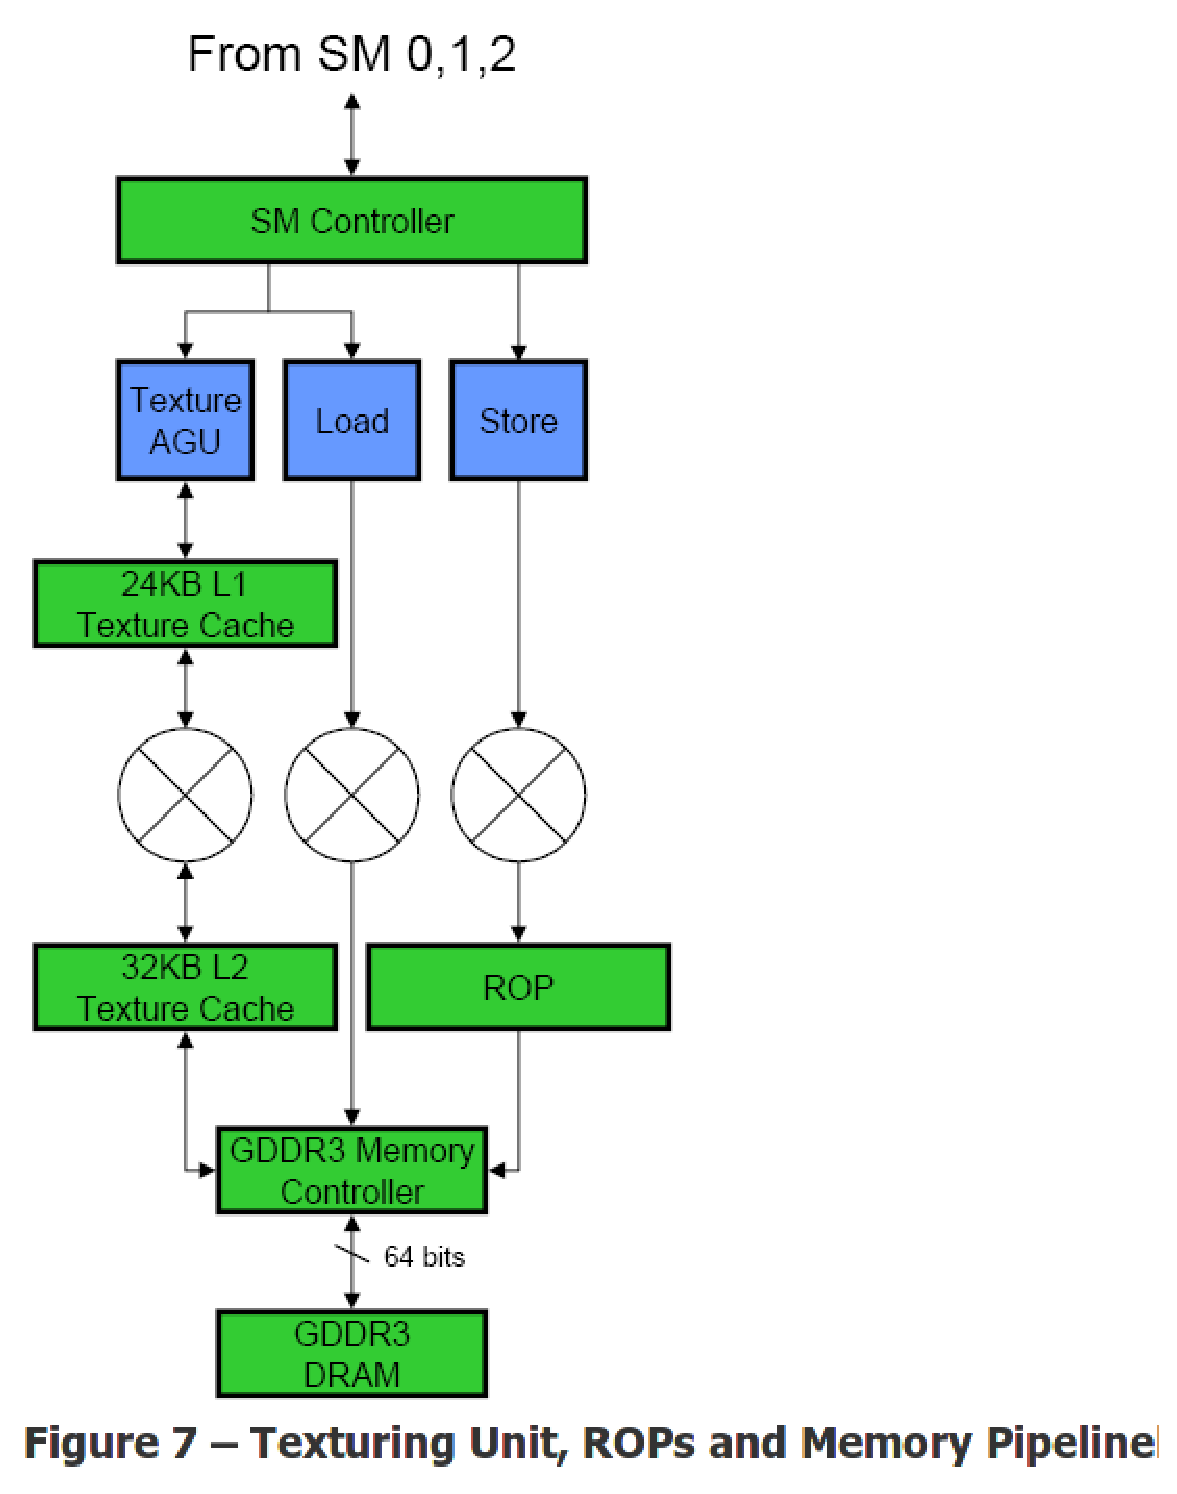
\includegraphics[height=7cm,
    angle=0]{./images/gt200_load.store.eps}}
  \caption{Texturing Unit, ROP and memory pipeline}
  \label{fig:gt200_load.store}
\end{figure}

Nvidia introduced a new generation of CUDA-capable GPU, called Kepler in 2013
(Chap.\ref{chap:Kepler}).

References:
\begin{itemize}
\item
  \url{http://benchmarkreviews.com/index.php?option=com_content&task=view&id=518&Itemid=72&limit=1&limitstart=2}

\item
  \url{http://www.firingsquad.com/hardware/Nvidia_gf100_architecture_overview/page3.asp}
\end{itemize}

\section{Thread hierarchy (Block \& Grid)}
\label{sec:block--grid}

In general, the instances of a kernel is executed by a number of
threads. To adapt the low granularity, threads are organized in
a hierarchical level as blocks and grids in a hierarchical structure as shown 
in Fig.~\ref{fig:grid_block}.

\begin{enumerate}
\item A {\bf thread block} has a number of threads, organized into 1D
  (vector), or 2D (grid, matrix), or 3D (cube). 
\item A {\bf grid} has a number of thread blocks, organized into 1D
  (vector) or 2D (grid, matrix). All blocks in the same grid has the
  same structures, i.e. equally-shaped thread blocks.
\end{enumerate}
\begin{figure}[hbt]
  \centerline{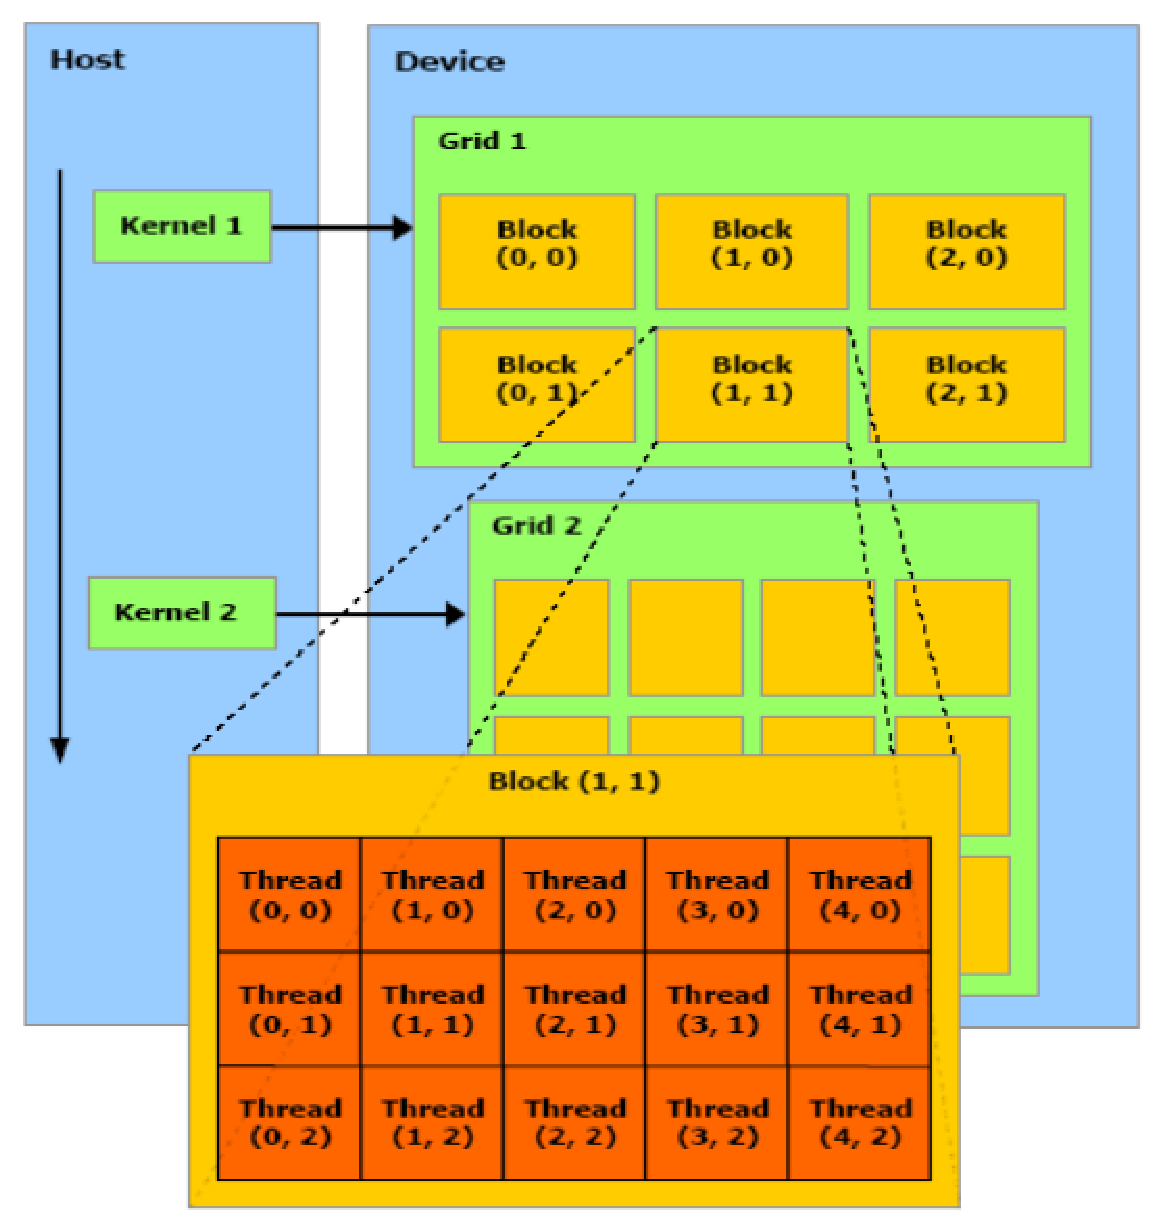
\includegraphics[height=7cm,
    angle=0]{./images/cuda_grid_block2.eps}}
  \caption{Example of a 2D grid and 2D block}
  \label{fig:grid_block}
\end{figure}

Each call to the kernel need to specify the execution configuration,
using chevron syntax, how the instances of the kernels - the
light-weight threads - are organized. The execution configuration has
two required information: grid structure and thread block
structure. This is a logical mapping to the data to be processed. The
data normally is an array in 1D, 2D, or 3D. Typically, one thread is
mapped to process one data element.


{\bf Example}: Add 2 vectors: if each thread will do the addition of
two corresponding entries of two vectors, you typically need to use 1D
thread blocks and if the length of the vector is smaller than the
maximum number of threads per block, you need to use only a single
thread block.
\begin{lstlisting}
! call the kernel VecAdd
call VecAdd<<<1, N>>>( n, a, x, y )
\end{lstlisting}
with
\begin{lstlisting}
attributes(global) subroutine VecAdd(N, A, B, C)
   real, dimension(N):: A, B, C
   integer i = threadIdx.x;

   if (i .le. N) C(i) = A(i) + B(i);
end subroutine
\end{lstlisting}
We will discover in detail later. Now, it's simply to know that, in
this example, the kernel has $N$ instances which will be processed by
a single block of $N$ threads.
\textcolor{red}{The limit of number of threads per block is 512 on
  C870 and C1060; and 1024 on Fermi}.
So, as we use only 1 thread block, the vector length should be less
than 512 (or 1024 if we use Fermi).

In many practical problems, the nature of the problem to be processed
in parallel is in the form of a matrix of 2D or 3D. In such problems,
the threads can be organized into a 2D or 3D {\bf thread block}. In
cases we need more than one thread block, the thread blocks can be
organized into a single {\bf grid} of 1D or 2D.

{\bf Example}: Matrix dot-product:
\begin{verbatim}
! element by element product
C(i,j) = A(i,j) * B(i,j)
\end{verbatim}
If the total number of elements of the matrix is smaller than 512 (or
1024 in Fermi), e.g. matrix size is 20x20, then we may need a single
2D thread blocks. 
\begin{lstlisting}
attributes(global) subroutine VecAdd(NX, NY, A, B, C)
   real, dimension(N):: A, B, C
   integer i = threadIdx.x;
   integer j = threadIdx.y;

   if (i .le. NX and j .le. NY) C(i,j) = A(i,j) + B(i,j);
end subroutine
\end{lstlisting}
However, it becomes more complicated when you need more than one
thread block (to be discussed later). 


\begin{framed}
  
\begin{itemize}
\item A grid is a 1D or 2D of blocks with maximum dim
  \begin{eqnarray}
    \label{eq:97}
    x_{max} \times y_{max} \times z_{max} = 65,535\times 65,535 \times 1
  \end{eqnarray}
\item A block is a 1D, 2D or 3D of threads with maximum dim
  \begin{eqnarray}
    \label{eq:98}
    x_{max} \times y_{max} \times z_{max} =  512\times 512 \times 64
  \end{eqnarray}

Suppose that the dim of a block is $x\times y\times z$, it is limited
by 
\begin{enumerate}
\item CC.1.x: $x\times y \times z \le 512$
\item CC.2.0: $x\times y \times z \le 1024$
\end{enumerate}
\end{itemize}

\end{framed}

There is a concept known as {\bf resident} thread/block (or activated
threads) which means the threads/blocks are currently utilizing the
hardware resource on a SM. Such resident threads of the blocks will be
executed in groups known as {\bf warps} by the SP cores. The excessive
blocks will be launched after the resident blocks are finished.  The
maximum number of active threads per
SM\footnote{this is different maximum number of threads per block,
  which is currently 512} is limited by the hardware
\begin{itemize}
\item 512 threads (Geforce 800)
\item 768 threads (Tesla 1st gen, i.e. CC.1.0, CC.1.1)
\item 1024 threads (Tesla 2nd gen, i.e. CC.1.2, CC.1.3)
\item 1536 threads (Fermi, i.e. CC.2.0)
\end{itemize}
Besides this limitation, there also other factor affecting to this
value, e.g. the number of registers used by each thread, the shared
memory used by each block. 

References:
\begin{itemize}
\item \url{http://llpanorama.wordpress.com/cuda-tutorial/} Good CUDA
  tutorial
\item \url{http://developer.Nvidia.com/object/cuda_2_3_downloads.html}
  CUDA resources
\item \url{http://sites.google.com/site/adelfahmed/Nvidia-cuda-experience}
\end{itemize}

% \subsection{Thread hierarchy}
% \label{sec:thread-hierarchy}

\subsection{Thread hierarchy in CUDA C/C++}
\label{sec:cudac_thread-hierarchy}

The main information is given in Sec.~\ref{sec:block--grid}. Here, we go
into details for CUDA C/C++.

\begin{table}[hbt]
\begin{center}
\caption{CUDA extension to C functional declaration}
\begin{tabular}{lcc} 
\hline
Example & Executed on & Callable from \\ 
\verb!__device__ float DeviceFunc()! & device & device \\
\verb!__global__ float KernelFunc()! & device & host \\
\verb!__host__ float HostFunc()! & host & host  \\
\hline\hline
\end{tabular}
\end{center}
\label{tab:TabLabel}
\end{table}

\subsection{1 grid, M threadblock (each with 1 thread)}

1 grid, M thread block, each of 1 thread
  \begin{lstlisting}
  mykernel<<<M, 1>>>();
  
  __global__ void mykernel() {
    int tid = blockIdx.x;
    
  }
  \end{lstlisting}
  The maximum number of thread blocks is 56,535 in Tesla.
  
\subsection{1 grid, 1 threadblock, N threads in 1D}

1 grid, 1 thread block, each of N threads (NOTE: we move from parallel
  blocks to parallel threads)
  \begin{lstlisting}
  mykernel<<<1,N>>>();
  
  __global__ void mykernel() {
    int tid = threadIdx.x ;
    if (tid < N) {
       ...
    }
  \end{lstlisting}

The maximum number of threads per block is 512 in Tesla, and 768 in Fermi.
From Kepler GPU, a single block we can have up to 1024 threads.

\subsection{1 grid, 1 threadblock (N threads in 2D)}

 1 grid, 1 thread block in 2D
  \begin{lstlisting}
 dim2 threads_per_block(32, 32);
 
  threads_per_block.x = 
  threads_per_block.y = 
  mykernel<<<1,block>>>()
  
  __global__ void mykernel() {
      int tidx = 
      int tidy = 
      int gtid = ...
  
  }
  \end{lstlisting}
  
  
\subsection{1 grid, M threadblock (each with N thread)}

1 grid, M thread blocks, each with N threads
  \begin{lstlisting}
  mykernel<<< (DIM + 127)/128, 128>>> ()
  mykernel<<< ceil(DIM/128), 128>>> ()
  
  __global__ void mykernel() {
    int tid = threadIdx.x + blockIdx.x * blockDim.x;
    
  }
  \end{lstlisting}
  with \verb!blockDim.x! keep the value of M.
  
  NOTE: Using 128 threads/block, each thread process a single element, then the
  maximum number of elements to be processed is 128*max(M)=8,388,480 elements in
  Tesla. To increase this limitation, one thread may process more than one
  element. This can be done by 
  \begin{itemize}
    \item split the long vector into chunk, each
    chunk is processed by a thread in 1D grid, 1D block. So, if there are more
    data, that thread will process data in the next chunk. The stride between
    two data elements to be processed by a single thread is 
    \verb!blockDim.x * gridDim.x!
    \begin{lstlisting}
    
    __global__ void add() {
       int tid = threadIdx.x + blockIdx.x * blockDim.x;
       while (tid < N) { // num elements
          c[tid] = a[tid] + b[tid]
          // jump to next chunk
          tid += blockDim.x * gridDim.x;
       }
    \end{lstlisting}
  \end{itemize}
  

\subsection{1D grid, 1D threadblock}

1D grid, 1D thread block
\begin{lstlisting}
__global__ myKernel(...) {
  int globalThreadID = threadIdx.x + blockDim.x * blockIdx.x;

  float x = input[globalThreadID];
  float y = func(x) ; //processing
  output[globalThreadID] = y;
}
\end{lstlisting}

\subsection{1D grid, 2D thread block, each thread block is 2D}

1D grid, 2D thread block, each thread block is 2D
\begin{lstlisting}
    dim3 blocks(ceil(DIM/16), ceil(DIM/16)) ;
    dim3 threads(16,16);

__global__ void mykernel() {
//global index x and y
   int x = threadIdx.x + blockIdx.x * blockDim.x;
   int y = threadIdx.y + blockIdx.y * blockDim.y;
//global linear offset
   int offset = x + y * blockDim.x * blockDim.y;
   
}   
\end{lstlisting}
In the example of calculating the sinusoidal function, with the origin is the
center of the iamge (DIM/2, DIM/2). We can do
\begin{lstlisting}
float fx = x - DIM/2;
float fy = y - DIM/2;
// the value of the sinusoidal at distance (fx,fy) to the origin
float d = sqrt(fx*fx + fy*fy);

// map that value to the color on the image
unsigned char grey = (unsigned char) (128.0f + 127.0f * cos(d/10.0f -
                ticks/7.0f) / (d/10.0f + 1.0f));
ptr[offset*4 + 0] = grey;
ptr[offset*4 + 1] = grey;
ptr[offset*4 + 2] = grey;
ptr[offset*4 + 3] = 255;
\end{lstlisting}
NOTE: We use multiplication, rather than power (\verb!^!) as it runs faster.




\subsection{1D grid, 3D threadblock}

\subsection{Mapping blockIdx and threadIdx to global threadID}
\label{sec:mapp-block-thre-1}

This is a widely used example: a big matrix is divided into submatrix,
each one of size \verb!BLOCK_SIZE!x\verb!BLOCK_SIZE!. So, we need
\begin{itemize}
\item put the data in each submatrix to the shared memory for fast
  process by a single thread
\item identify the starting index and ending index of the sub-matrix
\end{itemize}

\begin{lstlisting}
__global__ void myKernel(...) {

  //Block index
  int bx = blockIdx.x;
  int by = blockIdx.y;
  //Thread index
  int tx = threadIdx.x;
  int ty = threadIdx.y;

\end{lstlisting}


\subsection{Assign jobs to threads}
\label{sec:assign-jobs-threads}

Currently, each kernel is run by multiple threads organized as a single grid,
each grid has a structure of blocks, and each block has a structure of threads.


Each thread needs to know how to identify itself in the thread hierarchy using
two information: (1) block index, (2) thread index (in a particular block). The
previous section have introduced us this issue. In this section, we will learn
how to assign the data to a given thread for it to process.

\begin{figure}[hbt]
  \centerline{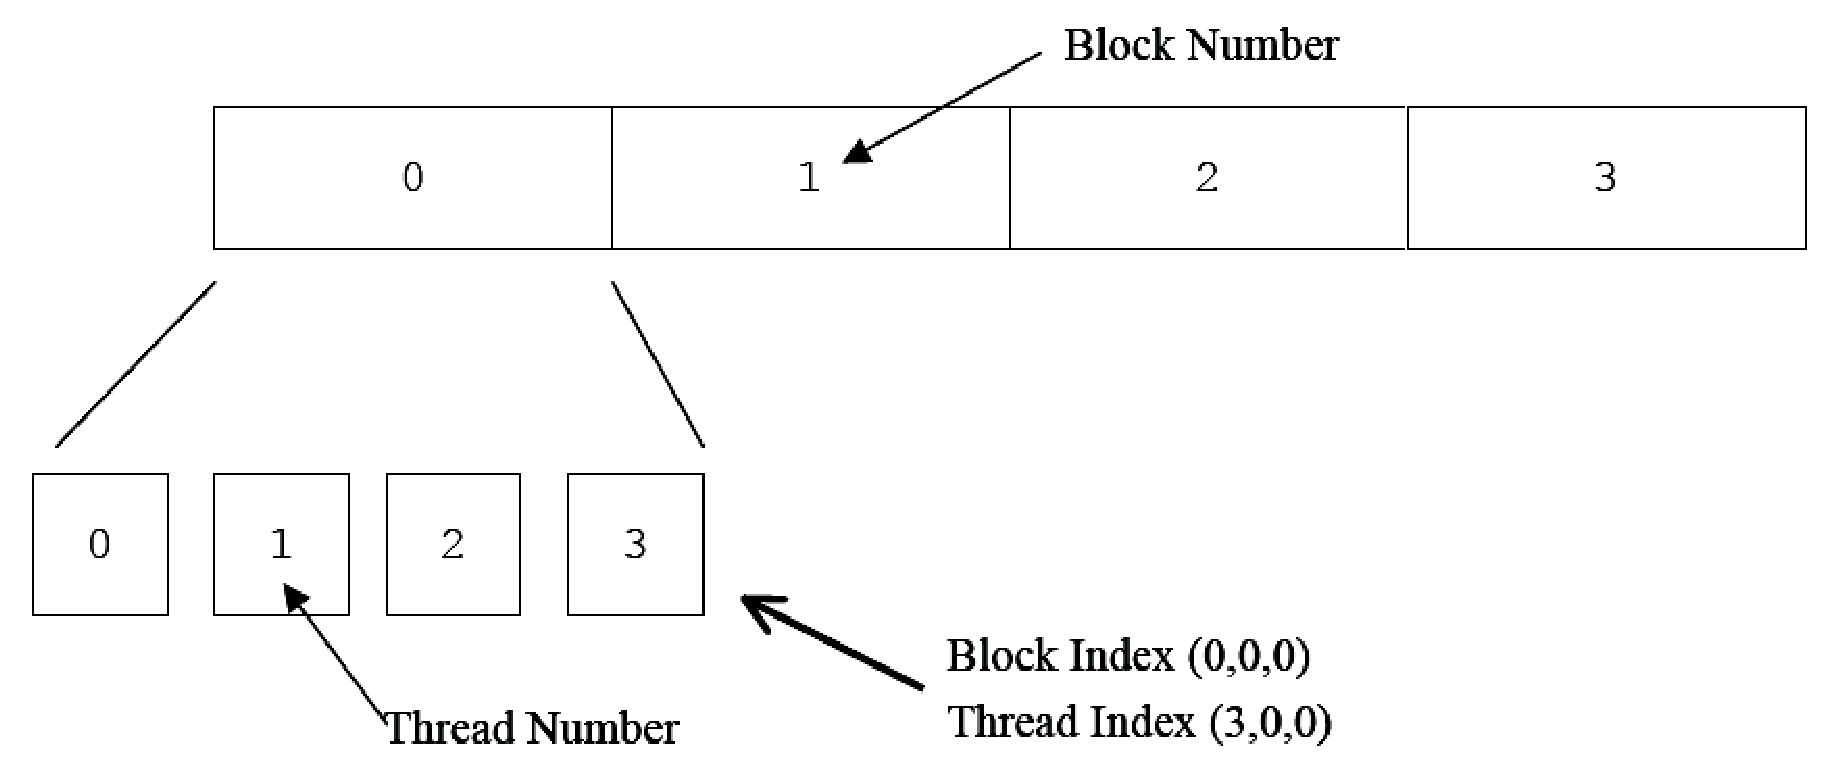
\includegraphics[height=3cm,
    angle=0]{./images/cuda_threadidx.eps}}
  \centerline{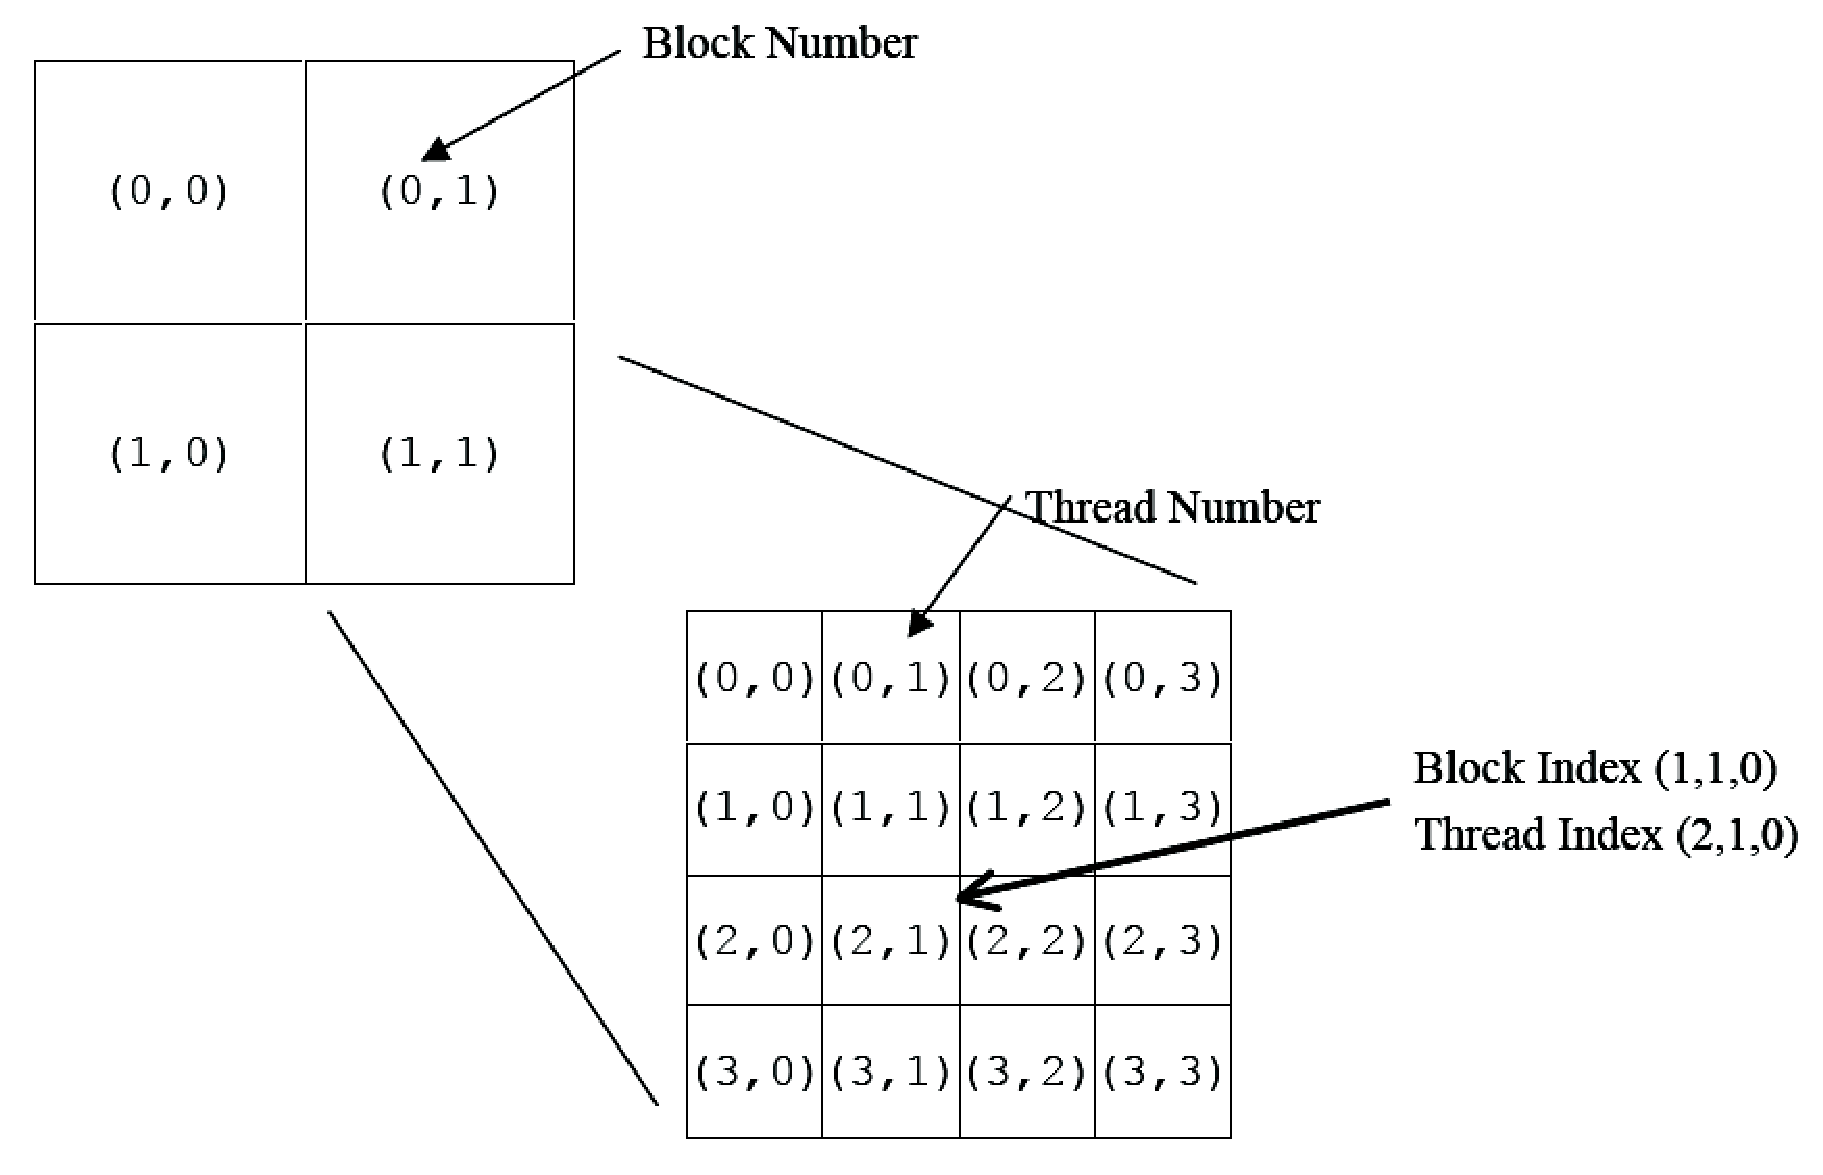
\includegraphics[height=5cm,
      angle=0]{./images/cuda_threadidx2.eps}}
  \caption{How to identify a thread (A) 1D grid, 1D block (B) 2D grid,
    2D block}
\label{fig:cuda_threadidx}
\end{figure}

Again, we will still use \verb!blockIdx! and \verb!threadIdx! to
determine the area of data that a thread is to work on. 


{\bf Example 0}: a square matrix multiplication problem
$\mathbf{P=M.N}$, the dimension of each matrix is \verb!Width!. We
assume the size of the matrix is a power of 2, e.g. \verb!Width=16!.
{\it The inner most loop iterates over variable $k$ and step through
  one row of $\mathbf{M}$ and one column of $\mathbf{N}$}. 
\begin{lstlisting}
for (int i = 0; i < Width; ++i) {
  for (int j = 0; j < Width; ++j) {
    float sum = 0;
    for (int k = 0; k < Width; ++k) {
      sum += M[i,k]*N[k,j]
    }
    P[i,j] = sum
  }
}
\end{lstlisting}
As the data is put in the memory, ultimately with a linear address,
and in row-major, we can access the element in a 2D array using a 1D
way as follows. This is the preferred way when accessing GPU memory.
\begin{lstlisting}
void MatrixMulHost(float *M, float*N, float* P, int Width) {
 for (int i = 0; i < Width; ++i) {
  for (int j = 0; j < Width; ++j) {
    float sum = 0;
    for (int k = 0; k < Width; ++k) {
      sum += M[i*Width+k]*N[k*Width+j]
    }
    P[i,j] = sum
  }
 }
}
\end{lstlisting}
with $i$ is row index of M, $k$ is column index of M and row index of
N, $j$ is the column index of N. 

{\bf Example 1}: If we use a single thread block, and each thread
process a single element, then the maximum size of the square matrix
is $16\times 16$. The reason is that the maximum number of threads in
a thread block (in Tesla 1,2) is 512, and $32\times 32$ exceeds this
value.
\textcolor{red}{If we want to multiple two square matrices of larger
  sizes, we need to use multiple thread blocks}.
\begin{lstlisting}
float * Md, Nd, Pd;
int size = Width * Width * sizeof(float);
cudaMalloc((void**) &Md, size);
cudaMalloc((void**) &Nd, size);
cudaMemcpy(Nd, N, size, cudaMemcpyHostToDevice);
cudaMemcpy(Md, M, size, cudaMemcpyHostToDevice);
//call kernel
call<<<...>>>MatrixMulKernel(Md,Nd,Pd, Width)

cudaMemcpy(P, Pd, size, cudaMemcpyDeviceToHost);
\end{lstlisting}
With the kernel, we no longer have the two outer loops. The row index
$i$ is mapped to \verb!threadIdx.y! and the column index $j$ is mapped
to \verb!threadIdx.x!.
\begin{lstlisting}
__global__ void MatrixMulKernel(float*Md, float*Nd, float*Pd, 
   int  Width) {
 int tx = threadIdx.x;
 int ty = threadIdx.y;
 float sum = 0;
 for (int k = 0; k < Width; ++k) {
   sum += Md[ty * Width + k] * Nd[k*Width+tx] 
 }
 Pd[ty*Width + tx] = sum;
}
\end{lstlisting}

{\bf Example 2}: We continue the previous example, the larger square
matrices are broken into smaller ones of size \verb!TILE_WIDTH!. Each
smaller square matrix is processed by a single thread block. So, the
suitable value for the size of the tile is \verb!TILE_WIDTH=16!. Now,
the x-index and y-index of the element for a thread is
\begin{lstlisting}
int tx = threadIdx.x;
int ty = threadIdx.y;
int bx = blockIdx.x;
int by = blockIdx.y;
int Row = (bx * TILE_WIDTH + tx)
int Col = (by * TILE_WIDTH + ty)
\end{lstlisting}
Again, we need to map the 2D index to 1D index.
\begin{lstlisting}
__global__ void MatrixMulKernel(float*Md, float*Nd, float*Pd, 
   int  Width) {

 ...
 float sum = 0;
 for (int k = 0; k < Width; ++k) {
   sum += Md[Row * Width + k] * Nd[k*Width+Col] 
 }
 Pd[Row*Width + Col] = sum;
}
\end{lstlisting}
and the execution configuration
\begin{lstlisting}
dim3 dimGrid(Width/TILE_WIDTH, Width/TILE_WIDTH);
dim3 dimBlock(TILE_WIDTH, TILE_WIDTH);
\end{lstlisting}

{\bf Example 3}: Continue the previous example, you realize that to
the two threads, say those to compute the element (x,y) and (x,y+1),
need to access the same row in matrix $\mathbf{Md}$. It means we need
to load twice the same data from global memory. We can enhance the
performing by loading only once to the shared memory and both thread
can use. NOTE: With NxN blocks, we can potentially reduce the traffic
by N. 

The question is can we load the whole matrices Md and Nd? Mostly, the
answer is NO, as the size of shared memory is too small. Even though
we cannot load the whole matrix, we however can load a submatrix which
is small enough to fit in the shared memory. Now, the shared memory to
hold a part of $\mathbf{Md, Nd}$ is called $\mathbf{Mds, Nds}$,
respectively. The submatrices are called {\bf tiles} whose size can
fit into the shared memory, each thread handle one element in the
tile. For simplification, we examine square matrices only and thus the
tiles are square matrices as well. 

As each thread handle one element in the tile, the tile size should
be maximum 16x16 which is known to give the best performance. 

. We can use $2\times 2$ tiles.
\textcolor{red}{In the simplest form, the tile dimensions equal those
  of the blocks. Then all threads in the block collaborate to load
  tiles of $\mathbf{Md,Nd}$ to shared memory}.
\begin{itemize}
\item Verify the reduction is by a factor of N if the tiles of size
  NxN.
\item In general, if an input matrix is of dimension N and the tile
  size is \verb!TILE_WIDTH!, then the number of phase is
  \verb!N/TILE_WIDTH! phases. Each phases focusing on a small subset
  of the input matrices which is called {\it locality}. When an
  algorithm exhibits locality, there's a chance to use small,
  high-speed memories to serve most of the accesses. Different phases
  use the same shared matrices \verb!Mds, Nds! declared as
\begin{lstlisting}
__shared__ float Mds[TILE_WIDTH][TILE_WIDTH];
__shared__ float Nds[TILE_WIDTH][TILE_WIDTH];
\end{lstlisting}

\item All threads in a single block will sequentially read the whole
  row block in $\mathbf{Md, Nd}$. With $2\times 2$ tiles, each thread
  access 4 elements of $\mathbf{Md}$ and 4 elements of $\mathbf{Nd}$.
\end{itemize}
\begin{lstlisting}
__global__ void MatrixMulKernel(....)


  int Row = ...;
  int Col = ...;

  float sum = 0;
  //Now it doesn't iterate the whole row/column of M/N, but a tile
  for (int k =0; k < Width/TILE_WIDTH; ++k)
    sum += Md[Row*Width + (m*
\end{lstlisting}


{\bf Example}: You have a data of size 800x800, you want to use 4
blocks to manage 4 non-overlapped subsets, each block manage a subset
data of size 400x400. If the block is a 2D of threads of size 4x4,
then each thread manage 100x100 piece, as shown 

\begin{figure}[hbt]
  \centerline{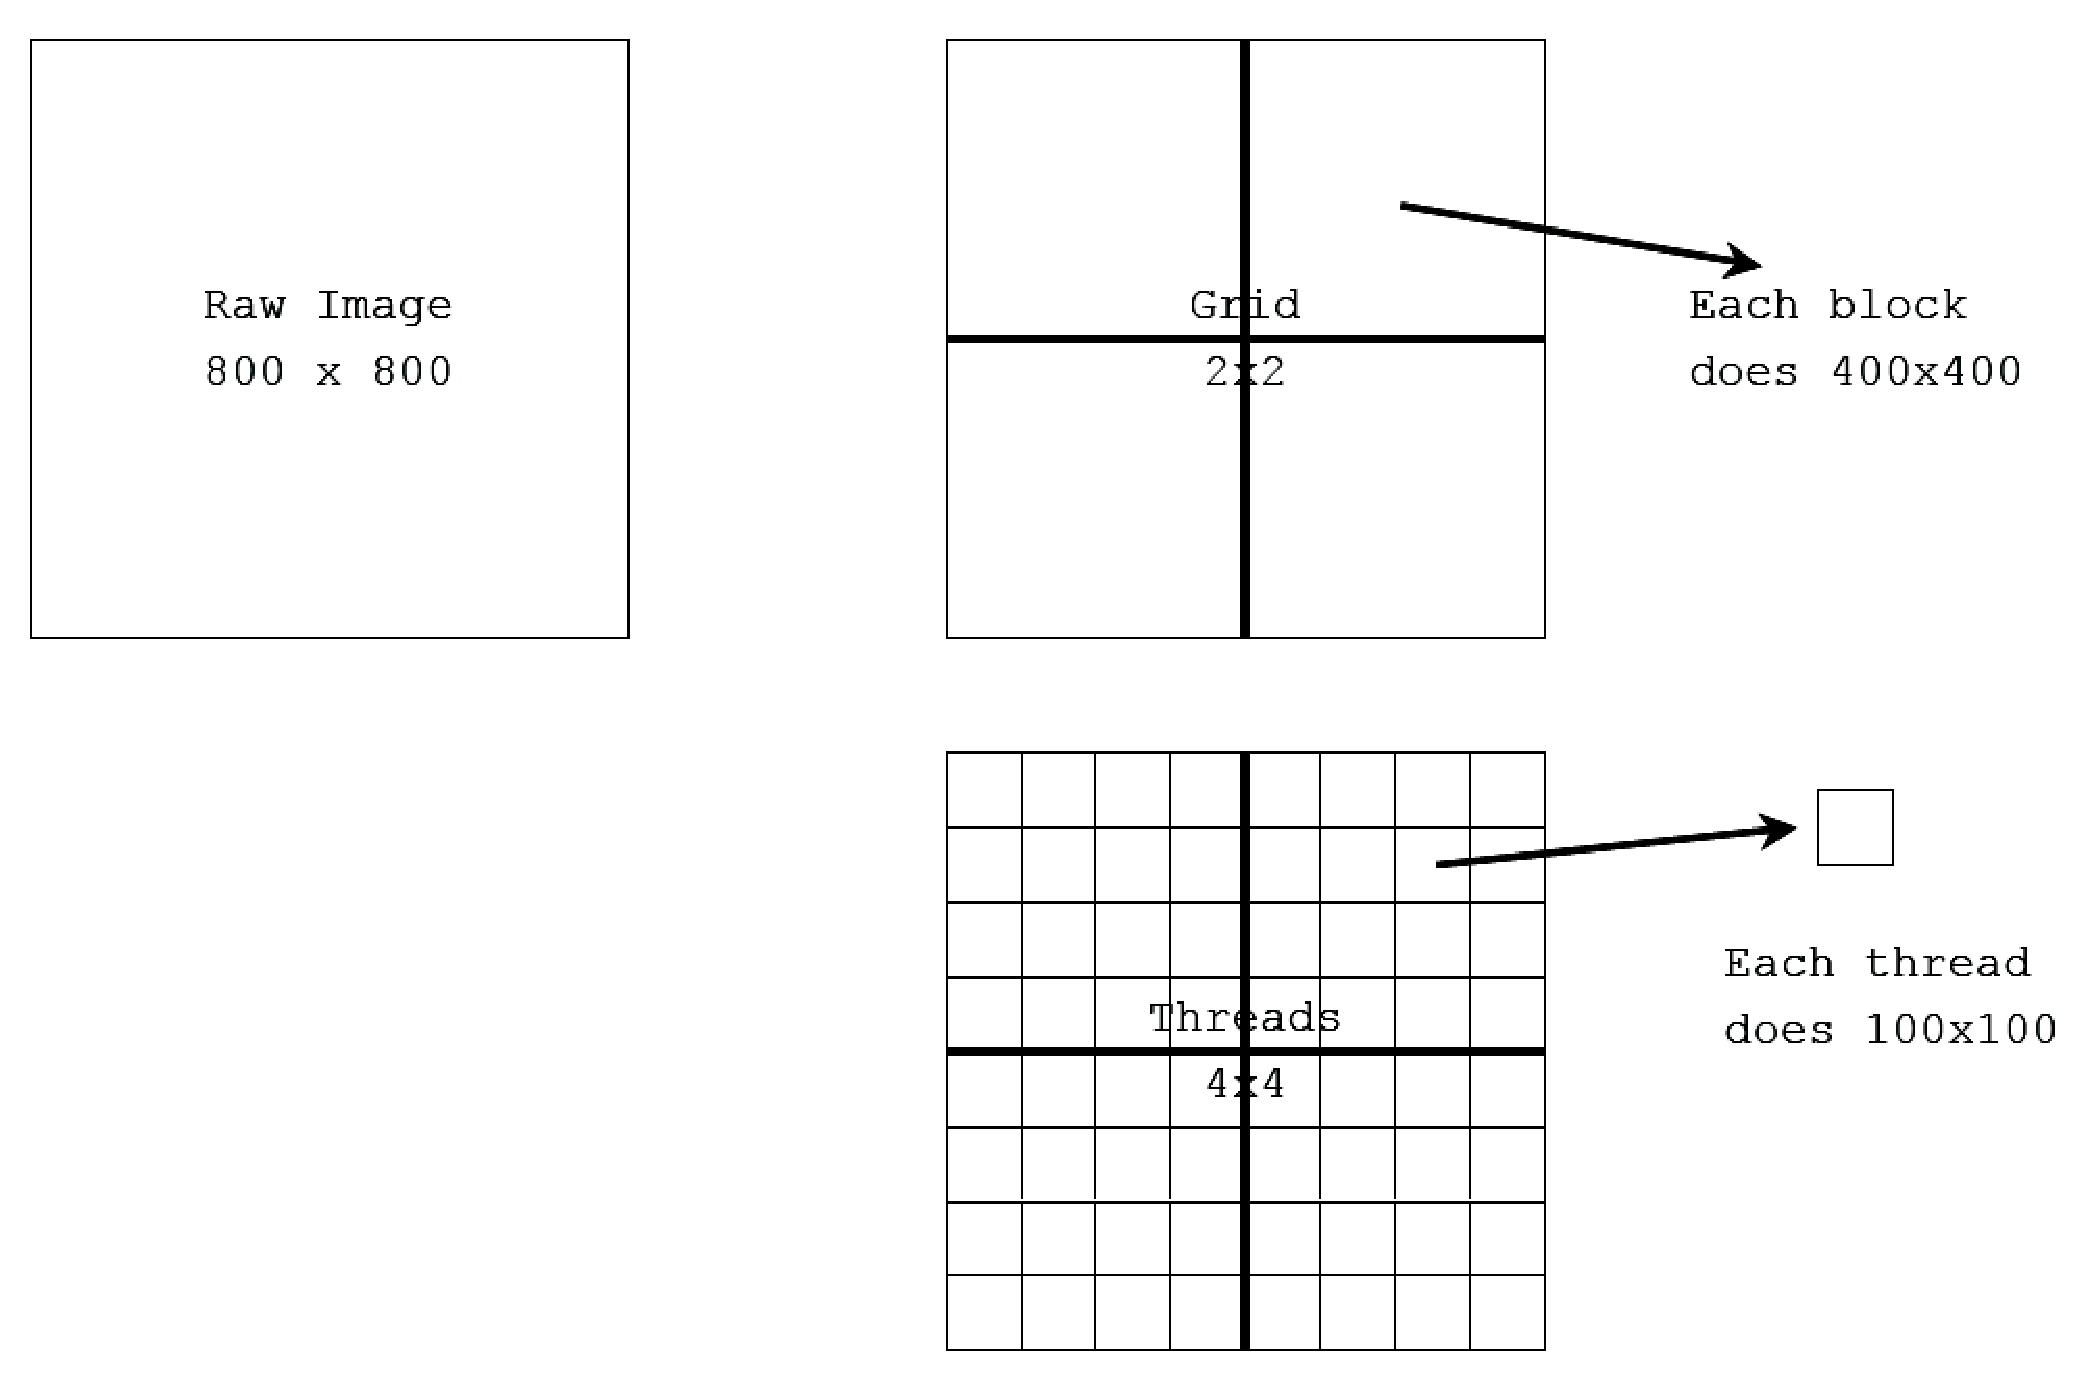
\includegraphics[height=5cm,
    angle=0]{./images/cuda_sample1.eps}}
\caption{CUDA sample 1}
\label{fig:cuda_sample1}
\end{figure}

{\bf Example}: You have a 2D image, each pixel is composed of 4 elements: R, G,
B, H. Each element is one byte, so you can 
\begin{lstlisting}
void kernel(unsigned char* ptr) {
  int tidx =    //col
  int tidy =    //row
  int offset = tidx + tidy * DIM ;
  ptr[offset*4 + 0] = 1; //R
  ptr[offset*4 + 1] = 2; //G
  ptr[offset*4 + 2] = 3; //B
  ptr[offset*4 + 3] = 4; //H
}
\end{lstlisting}


{\bf Example}: You have a data as a cube of size 300x300x300. As the
grid has maximum 2D, then you use 2D grid, e.g. 3x3x1. Then, each
block manage a subset of size 100x100x300. If the thread block, in
turn, has the size 3x3x1. then, each thread handle a subset of size
$\frac{100}{3}\times \frac{100}{3}\times 100$. For this situation, we
need to handle the irregular in data size. If we use threadblock of
size $33\times 33\times 100$, then, we have a small part has not been
processed. If we use threadblock of size $34\times 34\times 100$; then
the last threadblock will have less work to do, that's okay but we
need to control not to execute the code when the global thread index
is out of the range, as shown in Fig.~\ref{fig:cuda_sample2}.

\begin{figure}[hbt]
  \centerline{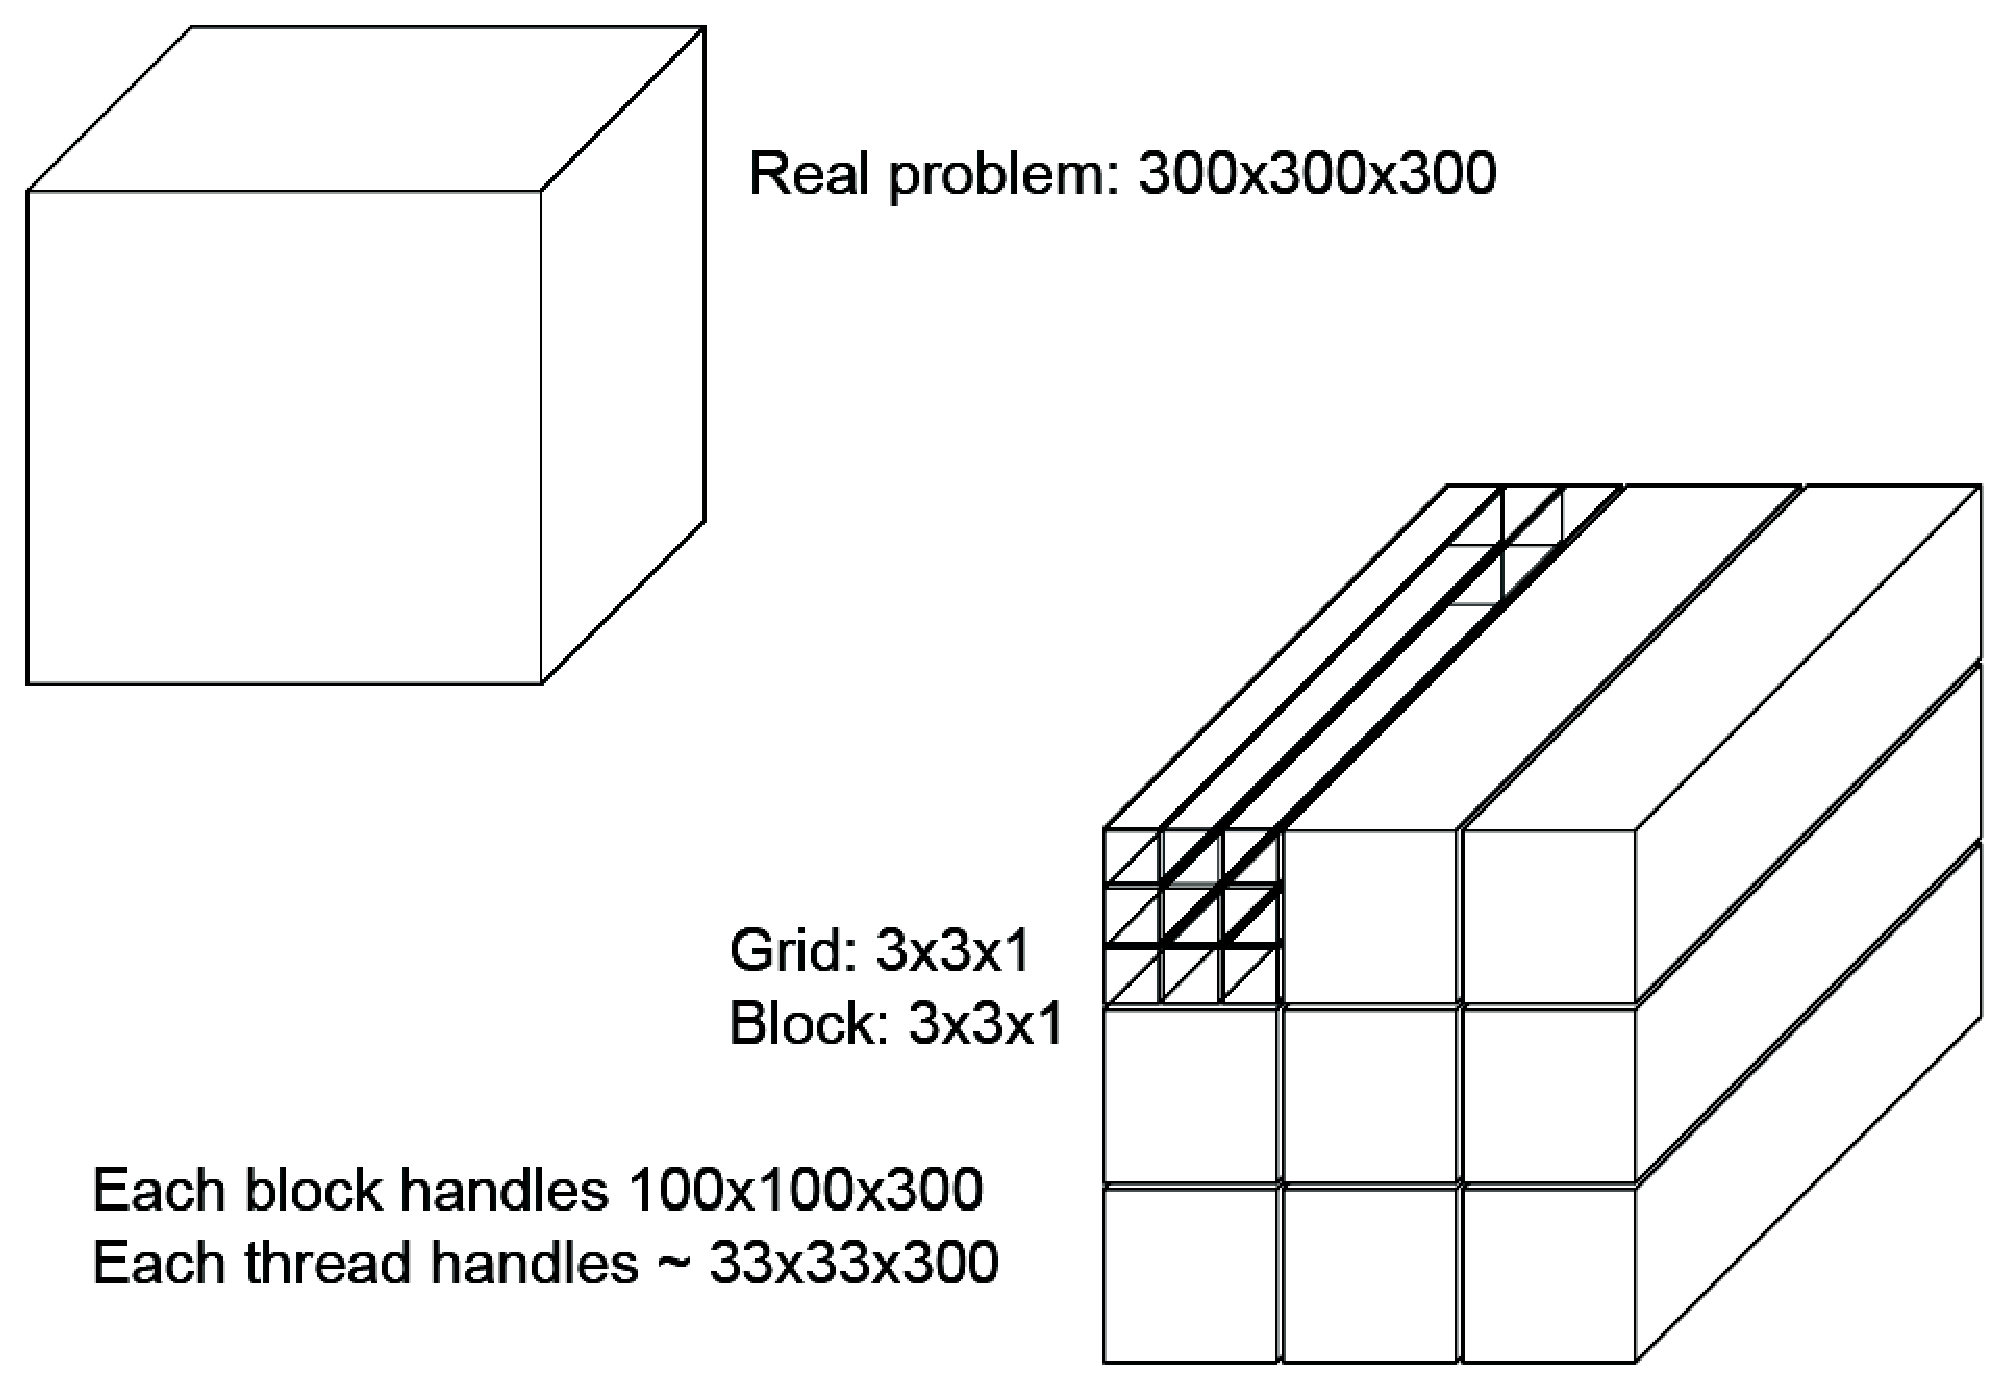
\includegraphics[height=5cm,
    angle=0]{./images/cuda_sample2.eps}}
\caption{CUDA sample 2}
\label{fig:cuda_sample2}
\end{figure}

{\bf IMPORTANT}: The total number of threads is
\begin{verbatim}
grid.x * grid.y * block.x * block.y * block.z
\end{verbatim}
In the above example, with the give hierarchical structure, the total
number of threads may not match up with the number of data elements
(with one thread process one data element). If you have more number of
threads or blocks than needed, you can turn a thread on/off by
comparing the global thread index with the number of data elements,
e.g.
\begin{lstlisting}[language=c]
// for vector origin data
__global__ void vcos( int n, float* x, float* y ) {
  int ix = blockIdx.x*blockDim.x + threadIdx.x;
  if( ix < n ) {
    y[ix] = cos( x[ix] );
  }
}

// for array origin data
__global__ void image_proc( int wd, int ht, float* x, float* y ) {
  if( ((blockIdx.x*blockDim.x+threadIdx.x) < wd)
    && ((blockIdx.y*blockDim.y+threadIdx.y) < ht) ) {
      :
  }
}
\end{lstlisting}

{\bf Example}: A better way to manage the situation in Example 2 is to
choose a different configuration for threadblock, i.e. use 1x1x3
rather than 3x3x1. Then, each thread manage a subset of size
100x100x100.

\begin{figure}[hbt]
  \centerline{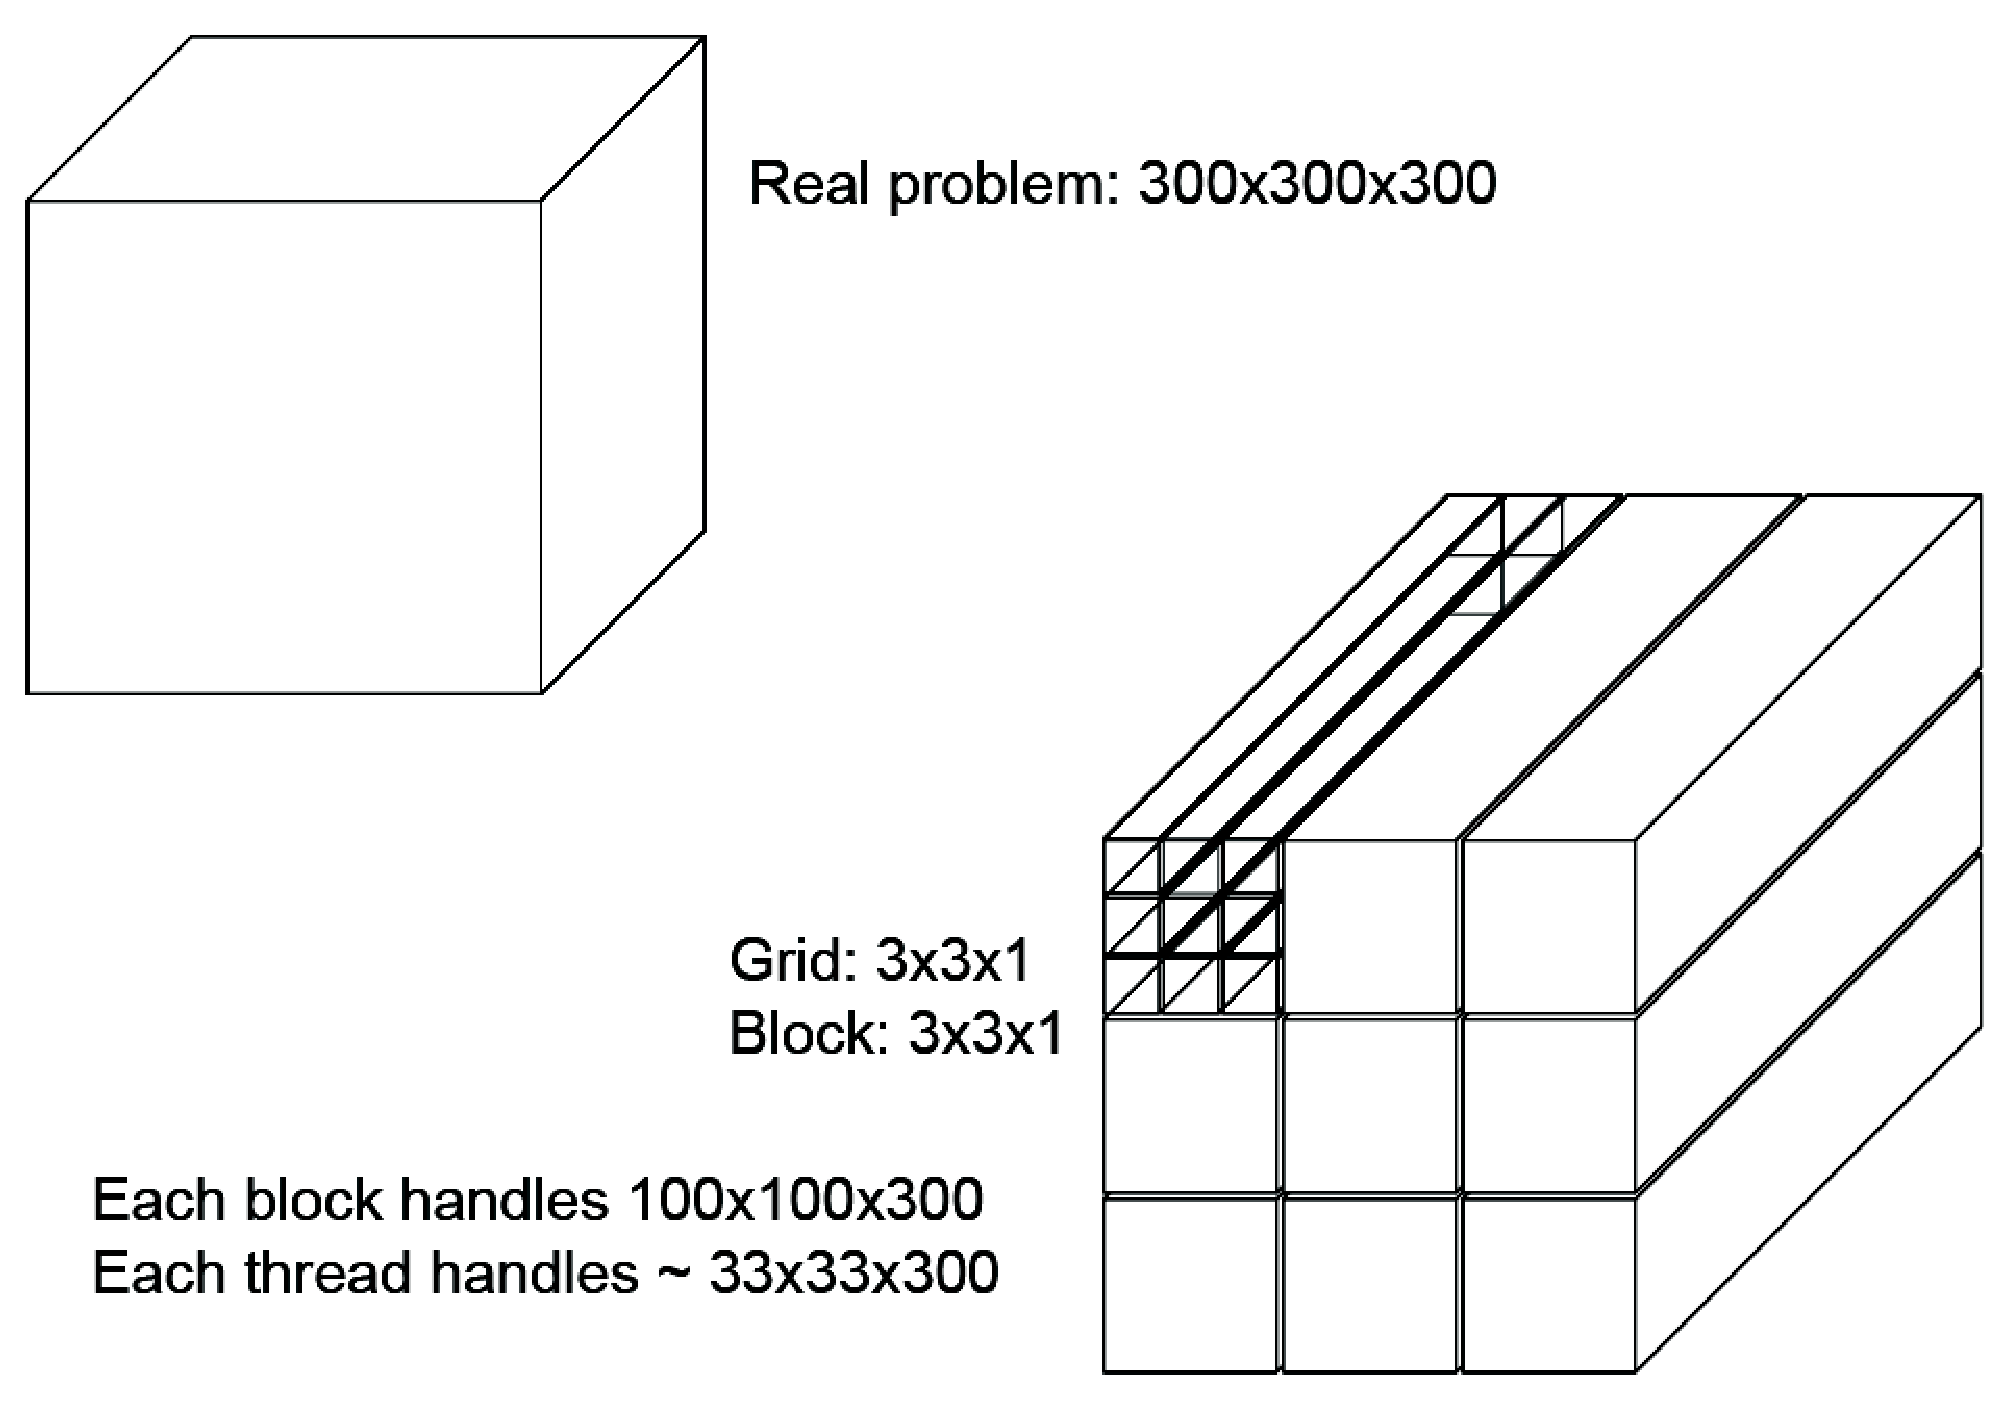
\includegraphics[height=5cm,
    angle=0]{./images/cuda_sample3.eps}}
\caption{CUDA sample 3}
\label{fig:cuda_sample3}
\end{figure}

\begin{framed}
  
{\bf NOTE}: Knowing the size of the data in advance will help
producing better GPU code.

\end{framed}

{\bf Example}: One thread process 1 data element

{\bf Example}: One thread process $64$ data elements
\begin{lstlisting}
__global__ void vcos( int n, float* x, float* y ) {
  int i;
  int ix0 = blockIdx.x*blockDim.x + 64*threadIdx.x;
  for(i=0;i<64;i++) {
    y[i+ix0] = cos( x[i+ix0] );
  }
}
\end{lstlisting}


The data is processed by a number of threads (instances of a kernel)
which can be organized into 1D, 2D, or 3D.
\begin{enumerate}
\item if grid is 1D and thread block is 1D
\begin{lstlisting}
// Ex.1: 
// launch bk thread blocks, each one has 256 threads (in 1D)
bk = (int)( n / 256 ) + 1;
vcos<<<bk,256>>>( n, dev_x, dev_y );


__global__ void vcos( int n, float* x, float* y ) {
  int ix = blockIdx.x*blockDim.x + threadIdx.x;
  if (ix < n) {
    y[ix] = cos( x[ix] );
  }
}
\end{lstlisting}
Each thread has a unique \verb!threadIdx.x! and \verb!blockIdx.x!, a
thread can also get access to \verb!blockDim.x! and \verb!gridDim.x!
(for more complicated grid structure).

\item if grid is 2D and thread block is 2D: there is a new type
  \verb!uint3!. 
\begin{lstlisting}
uint3 m,n;
m = make_uint3(128,128,1);
n = make_uint3(32,32,1);
vcos<<<m,n>>>( n, dev_x, dev_y );

// or declare like this
uint3 m,n;
m.x=128; m.y=128; m.z=1;
n.x=32; n.y=32; n.z=1;
\end{lstlisting}

Due to the limits of the number of threads running simultaneously
\end{enumerate}

Here is the sample that show how to share the work to threads:
\begin{enumerate}
\item if grid is 1D and thread block is 1D
\begin{lstlisting}
/* Example 1 - simple: 
     grid has 1 threadBlock;
     threads in a block are organized in 1D
e.g.: add 2 vectors whose length < 512, so we need 
     only 1 threadblock
*/
VecAdd<<<1,N>>>(N,C,A,B);

.........
__global__ void function VecAdd(int N, float C[N],
                float A[N], float B[N]) {
  int i;
  i = threadIdx%x;
  C[i] = A[i] + B[j];
}
\end{lstlisting}
\begin{lstlisting}
/* Example 2 - more complicated
   grid has 1D of blocks
   threads in a block are organized in 1D
e.g.: add 2 vectors whose length > 512, so we need 
      more than 1 threadblock
*/
VecAdd<<<N/512, 512>>>(N,C,A,B);


__global__ void function VecAdd(....) {
/* 1D threadBlock map to global thread index i
  the index of the thread related to its threadId
*/
  i = (blockIdx%x-1) * blockDim%x + threadIdx%x;
  if (i <= N) {
    C[i] = A[i] + B[i];
  }
}
\end{lstlisting}

\item if grid is 1D and thread block is 2D of size $(D_x,D_y)$
\begin{lstlisting}
// Example 1 - simple:
//          grid has 1 threadblock, 
//          threads in a threadblock is in 2D
//e.g.: add 2 matrices whose number of elements M*N < 512, 
//      so we need only 1 threadblock
dim3 dimBlock(Dx,Dy) 
call MatAdd<<<1,dimBlock>>>(A,B,C,Dx,Dy)
...............
attributes(global) subroutine MatAdd(A,B,C,M,N)
  real, dimension(M,N) :: A,B,C
  integer :: M,N
i = threadIdx%x;
j = threadIdx%y;
if (i .le. M .and. j .le. N)
   C(i,j) = A(i,j) + B(i,j)
endif
\end{lstlisting}

\begin{lstlisting}
// Example 2 - more complicated
//e.g.: add 2 matrices whose size is unknown, i.e. M*N can be > 512
//      we need more than 1 threadblock
dim3 dimGrid((N + dimBlock.x - 1) / dimBlock.x, &
    (N + dimBlock.y - 1) / dimBlock.y);
dim3 dimBlock(20, 20);

call MatAdd<<<dimGrid, dimBlock>>>(A, B, C);
.....

\end{lstlisting}

\item if grid is 1D and thread block is 3D of size $(D_x,D_y,D_z)$
\item if grid is 2D and thread block is 1D
\item if grid is 2D and thread block is 2D
\item if grid is 2D and thread block is 3D
\end{enumerate}

\subsection{Thread synchronization}
\label{sec:thre-synchr}

During the execution of threads, if you want all threads in a single
block, to wait for each other at a given point, you can call
\verb!__syncthreads()!.

\begin{lstlisting}
... step 1...
__syncthreads();
... step 2...
\end{lstlisting}
Normally, we load data (data copy to shared memory) in step 1 to avoid
read-after-write hazard for shared memory, as well as for device memory.

\begin{framed}
  \verb!_syncthreads()! simply allows you to set a synchronisation
  point, and no code after that point will be executed (barring,
  perhaps, code related neither to the shared memory nor the device
  memory) until all threads in the block have finished executing all
  previous instructions.
\end{framed}

Read this: \url{http://www.beyond3d.com/content/articles/12/4}



\subsection{Chevron syntax: <<< dim3, dim3>>>, <<<int, int>>>}
\label{sec:chevron-syntax}
\label{sec:dim3}

A kernel is invoked with many thread blocks of the same
size. Sect.~\ref{sec:thread-blocks} describes the structure of a
thread block. The thread blocks are organized in 1D, 2D (or in Fermi,
added 3D) structure. So, to call a kernel, you need to pass the
information about the number of threads in a block, and the number of
blocks in a grid, and (optionally) the number of bytes dynamically
allocated in shared memory. This is specified using

\begin{lstlisting}
dim3 numBlocks(8,8);
dim3 threadsPerBlock(8,8,8);
myKernel<<<numBlocks, threadsPerBlock>>>(args);
myKernel<<<16,64>>>(args);


// call 
MyKernel<<<grid_size, block_size [, mem_size]>>>(...)
\end{lstlisting}
This syntax is known as the {\bf chevron syntax}.  A kernel is dispatched if
both are true
\begin{enumerate}
\item Resources are available
\item Preceding calls in the same stream have completed
\end{enumerate}

CUDA threads are created by functions called kernels which must be
\verb!__global__! (Sect.\ref{sec:__global__functions}).
Kernels are launched with an extra set of parameters enclosed by
\begin{verbatim}
 <<< first, second >>>
\end{verbatim}.
The first argument is a dim3 representing the grid dimensions and the second is
another dim3 representing the block dimensions (Sect.\ref{sec:dim3}).
ou can also use ints instead of dim3s, this will create a Nx1x1 grid).



In the simplest case, i.e. \verb.<<<K, L >>>. with $K=1$, and the number of
thread in each thread block, e.g. $L=N$. Here, both K and L are integer values
as grid is 1D and thread block is 1D. However, in general, when the threads is
organized into 1D, 2D or 3D; or the thread blocks is organized into 1D or 2D,
you need to use some builtin variables of type {\bf type(dim3)}.

\begin{enumerate}
\item \verb.threadIdx. (type: type(dim3)): contains block thread index
  within each block
\item \verb.blockDim.: contains the dimension for each thread block
  and is the same at all threads in the grid.
\item \verb.blockIdx.: contains the block index within a grid (NOTE:
  we always have \verb. blockIdx%z=1.) and is the same for all threads
  in the same block
\item \verb.gridDim.: contains the dimension for the grid (NOTE: we
  always have \verb. gridDim%z=1.) and is the same for all
  threads in the grid.

\item \verb.warpSize. (type: integer(4)): contains the number of
  threads in a single warp (NOTE: currently, threads are executed in
  groups of 32, called {\bf warps}, so \verb.warpSize=32. always)
\end{enumerate} 

{\bf NOTE}: These predefined variables are intended to be used in
device subprograms only, i.e. they are inaccessible in any host
subprograms



One very important question you may ask is
\textcolor{red}{What is the maximum number of threads in a thread
  block, or in a grid?}
- Such numbers are limited by the
\hyperref[sec:compute-capability]{compute capability} and we will
learn in a different section. With Compute Capability 1.3 (CC 1.3),
the maximum number of threads in a thread block is 512.



\section{Host functions, Kernel (global function) and Device functions}

\begin{enumerate}
  \item host code (i.e. code running on CPU)
  
  \item device code (i.e. code running on GPU, but must be called from a host code - using a special syntax)
    
  \item kernel code (i.e. code running on GPU, and must be called from a device code - as a regular function)
\end{enumerate}

Nvidia extends C language, i.e. if you compile your code using \verb!nvcc!, it recognizes the following new 
keywords which is specified at the beginning of a function definition:

\begin{verbatim}
__host__ - Runs on the CPU, called from the CPU.
      This is the traditional function as we often develop.
      This is called host function

__global__ - Runs on the GPU, called from the CPU. Executed with <<<dim3>>> arguments.
      This is called kernel, or global function

__device__ - Runs on the GPU, called from the GPU. Can be used with variabiles too.
      This is called device function.
\end{verbatim}

\subsection{Host functions}
\label{sec:host-function}

Host functions are functions that are executed on the host-side, i.e. the CPU.
By default, a function is a host function.
We can explicitly tell the compiler to generate a host copy of a function by
adding \verb!__host__! keyword.

\subsection{GPU-friendly functions}
\label{sec:CUDA-friendly-functions}

A GPU-friendly function is a function that runs on GPU, however depending upon
where it is evoked, it falls into one of the two following categories
\begin{verbatim}
__global__

__device__
\end{verbatim}


We can tell a compiler, e.g. nvcc, to generate two copies of a function as both a host code and device code 
\begin{verbatim}
#ifdef __CUDACC__
#define CUDA_CALLABLE __host__ __global__
#else
#define CUDA_CALLABLE
#endif


CUDA_CALLABLE  void my_function(void)
{
}

int main(void) {

#ifdef __CUDACC__
  my_function<<<1, 1>>>();
#else
  my_function();
#endif

}
\end{verbatim}

NOTE: The special macro \verb!__CUDACC__! (Sect.\ref{sec:__CUDACC__-macro}.

Such code must be compiled using \verb!nvcc! which will split parts
\begin{enumerae}
  \item device functions to be processed by Nvidia compiler
  
  \item host functions to be processed by stanard host compiler, e.g. gcc, cl.exe
\end{enumerae}

\subsection{-- Global function (aka kernels): defined using \_\_global\_\_}
\label{sec:__global__functions}

A global function is a function defined using \verb!__global__! keyword, and must return \verb!void!.

NOTE: The keyword \verb!__global__! can be used in C function or C++ class
method (support for C++11 is available from CUDA 7.0).

\begin{verbatim}
__global__ void addVectors(float* vec1, float* vec2, float* result) {
    ...
}
\end{verbatim}
Global functions are also called CUDA "kernels". It's the functions that you may call
from the host function (Sect.\ref{sec:host-subprogram}) using CUDA kernel call semantics (<<<...>>>).
This is known as the chevron syntax - Sect.\ref{sec:chevron-syntax}.
\begin{verbatim}
addVectors<<< no_of_blocks , no_of_threads_per_block>>>(...);
\end{verbatim}

So, a CUDA kernel is just a function that is executed in parallel by N different
CUDA threads (Sect.\ref{sec:threads} describes how CUDA threads for a CUDA
kernel are organized). When kernel is called we have to specify how many threads
should execute our function, using the above chevron syntax. Each thread, as
identified by its unique thread id, executes the kernel instance.


CUDA kernel, as running on GPU, can access to the data on GPU via a number of options
\begin{enumerate}
  \item if data is on global memory: the data must be passed via kernel argument
  
  \item if data is defined as constant: the data must be defined at global level, and then can be accessed directly from within the kernel
  
\end{enumerate}

CUDA kernels can also have access to 4 (implicitly defined) variables that give information about a thread’s
location in the grid

\begin{verbatim}
threadIdx.[xyz] represents a thread’s index along the given dimension.

blockIdx.[xy] represents a thread’s block’s index along the given dimension.

blockDim.[xyz] represents the number of threads per block in the given direction.

gridDim.[xy] represents the number of blocks in the given direction.
\end{verbatim}

As each instance of the kernel is a CUDA thread, by using these variables we can
tell what thread the kernel instance belongs to and thus, can identify the data index that the kernel instance to handle.

A unique id for each thread indexed from 0 to N where N is the total number of
threads. For a one dimensional grid and a one dimesional block this formula is
blockIdx.x * blockDim.x + threadIdx.x.

\begin{verbatim}
int main() {
    ...
    addVectors<<<1, N>>>(vec1, vec2, result);
    ...
}

__global__ void addVectors(float* vec1, float* vec2, float* result) {
    int index = threadIdx.x;
    result[index] = vec1[index] + vec2[index];
}
\end{verbatim}


\begin{itemize}
\item Kernel function: \verb!__global__!: must return type
  \verb!void!, if the function get error, you must provide the error
  message/value some way.
\begin{lstlisting}
__global__ void acos_main (struct acosParams parms){
  int i;
  int totalThreads = gridDim.x * blockDim.x;
  int ctaStart = blockDim.x * blockIdx.x;
  for (i = ctaStart + threadIdx.x; i < parms.n; i += totalThreads) {
     parms.res[i] = acosf(parms.arg[i]);
  }
}
\end{lstlisting}
As you cannot pass CPU pointer to the kernel function, then you must
(1) save the error value to the GPU, (2) copy it back to CPU. As there
are many thread doing the same code, we need to control whether all
threads writing to the same error code area.

\item Device function: to be called from a Kernel function only,
  i.e. callable from device. It must be no recursion, no static
  variable within function
\begin{lstlisting}
__device__ float deviceFunction(...) {

}
\end{lstlisting}

\end{itemize}

The syntax to call a GPU kernel is {\it chevron syntax}. Kernel
calling does not directly report an error; instead, you can call to
\verb!cudaGetLastError()! to check for successfullness. 
\begin{lstlisting}
cudaError_t err;
func_name<<<grd,blk>>>( arguments );
err = cudaGetLastError();
if( err != cudaSuccess ) {
   /* something bad happened during launch */
}
\end{lstlisting}

However, error handling is not that simple. 

\subsection{-- Device functions \_\_device\_\_}
\label{sec:__device__functions}

Device functions can only be called from other device or global functions.
\verb!__device__! functions cannot be called from host code.

As calling from inside a kernel, which alreadys on the device-side, and you
don't have to set the kernel settings.

You can also "overload" a function, e.g : you can declare 
\begin{lstlisting}
void foo(void) 
\end{lstlisting}
and
\begin{lstlisting}
__device__ foo (void)
\end{lstlisting}
, then one is executed on the host and can only be called from a host function.
The other is executed on the device and can only be called from a device or
kernel function.


\subsection{Predefined variables}
\label{sec:predefined-variables}

\begin{lstlisting}
dim3 threadIdx; 

dim3 blockIdx; 

dim3 blockDim;
\end{lstlisting}


\section{How to organize CUDA code}


C codes with CUDA has file extension as ``.cu'' and must be compiled
with \verb!nvcc!, a compiler driver that invokes necessary tools
(cudacc, g++, cl, ...) to compile the code.

Separate compilation is an integral part of the C and C++ programming languages
which allows portions of a program to be compiled into separate objects and then
linked together to form an executable or library.

\begin{mdframed}

REMINDER: A common way to organizes functions in C++ is to put them into a
class: define all member functions of a single class in one or more .cpp source
files, and compile each .cpp source file into a separate .o object file.


COMPILATION STEP: Other classes and functions may call these member functions from anywhere in the
program by including the class header file; the function implementation is not
needed to compile another function that calls it

LINKING STEP (to generate library or final executable file): After compiling all
code, the linker connects calls to functions implemented in other files as part
of the process of generating the executable.

\end{mdframed}

Starting with CUDA 5.0, separate compilation and linking are now important tools
in the repertoire of CUDA C/C++ programmers.



References: \url{https://devblogs.nvidia.com/separate-compilation-linking-cuda-device-code/}




\section{CPU pointer vs. GPU pointer}
\label{sec:cpu-pointer-vs}

In CUDA C programming, pointers are extremely popular. Pointers are just memory
locations whose contents is another memory addresses.  

The pointer is always on the CPU-side, but the content, i.e. the address that is
stored by the pointer, can be GPU-memory address, or CPU-memory address.
If the address in GPU-memory address, we call the pointer is GPU pointer; and
otherwise, we call it CPU pointer.

There is no way to discriminate CPU pointer and GPU pointer, or we cannot tell
if a address that a pointer content is device memory or host memory.

From the host side,  it is illegal to dereference a GPU pointer, i.e. the
host-side pointer whose content is a GPU-memory address
\begin{verbatim}

&coeffs 
    would imply the address of the symbol in host memory not GPU memory
\end{verbatim}
Also dereferencing a CPU pointer on GPU will likely crash.

In the next sections, how we handle GPU pointer, depending upon the GPU architectures
\begin{enumerate}
  \item pre-Fermi GPU: Sect.\ref{sec:GPU-pointer-pre-Fermi}
  
  \item Fermi GPU+ : Sect.\ref{sec:GPU-pointer-post-Fermi-pre-Kepler}
\end{enumerate}

\subsection{-- pre-Fermi}
\label{sec:GPU-pointer-pre-Fermi}

In pre-Fermi generations of CUDA-capable GPU, unlike pointer in host memory,
pointer in device memory use physical memory address. It means that the content
of the pointer is the physical address on GPU. pre-Fermi GPUs do not implement a
virtual memory mechanism.

As a result, this is the common steps in host code: 
\begin{enumerate}

\item (optional) select a GPU

\item allocate device memory, i.e. accessing via GPU pointer

\item allocate CPU data of the same size of device memory

\item initialize data via this CPU data

\item copy data from host to device memory

\item launch the kernel(s)

\item once needed, copy data from the device to host

\item at the end, deallocate data on device memory, and on CPU memory 
\end{enumerate}

Mostly, we can access data on the device memory by assigning the data to it or
copying the data from it. We cannot modify the data on the device directly using
arithmetic operations. On the other hands, we cannot modify data on the host
memory from a kernel function.

In GPU, constant memory (Sect.\ref{sec:constant-memory}), Shared memory, Local
memory and Global memory form their own address space. Developers can only
create and access pointers GPU global memory, but not others. Location of data
on constant memory, shared memory, local memory is hardware-managed.


\subsection{-- post-Fermi}
\label{sec:GPU-pointer-post-Fermi-pre-Kepler}

Since Fermi generation with CUDA 4.0+, CUDA now implement virtual address
spaces, although the hardware does not support as rich a feature set as those in
CPUs (Sect.\ref{sec:memory-on-CPU-side}).

Using virtual address space, GPUs do enforce memory protections, so CUDA
programs cannot accidentally read or corrupt other CUDA programs’ memory or
access memory that hasn’t been mapped for them by the kernel mode driver.

\textcolor{red}{LIMITATION}: But GPUs do not support demand paging, i.e. you
cannot allocate/request more than the physical memory limit. So every byte of
virtual memory allocated by CUDA must be backed by a byte of physical memory,
i.e. you cannot allocate more than the physically available memory on GPU.

Remember that in the previous generation of GPU, users need to manage a pair of
pointers (CPU, GPU) for one set of data; and users need to manually copy data
back and forth if data is updated on one side, and then is needed on the other
side. To avoid that, CUDA 4.0 supports unified virtual addressing (UVA) which 
provides a virtual memory space that both CPU and GPU can access (Sect.\ref{sec:UVA}).

UVA allows GPU pointers and CPU pointers to be on the same virtual addressing
space. So, the job of managing where buffer lives (on host or device side) is
transfered to the CUDA driver, which free programmers to focus on other aspects
of programming. Also, pointers for global memory and shared memory are
equivalent.

Since each GPU has its own memory and address translation hardware, the CUDA
address space is separate from the CPU address space where the host code in a
CUDA application runs.




\subsection{-- post-Kepler CUDA 6.0}

Single pointer for CPU and GPU. However, as it does not allow page-faults on GPU
side, before kernel launch, it needs to update all pages on GPU-side.

\begin{verbatim}

// the pages are populated in GPU memory
cudaMallocManaged(&ptr, ...); 


// at this access, CPU page fault occurs, i.e. the CPU page directory has no information yet
// then: 
//   a memory is allocated on CPU-memory, and data migrates to CPU
//   and the CPU page directory get updated
*ptr = 1; 

// at kernel launch: it triggers bulk page migrations, i.e. 
//       the whole data migrates to CPU
//       if the data is big, i.e. span multiple pages, then all the pages are migrated
qsort<<<...>>>(ptr);
\end{verbatim}

On pre-Pascal you can use zero-copy but the data will always stay in system memory

\subsection{-- post-Pascal CUDA 6.0}

Pascal has a {\bf Page Migration Engine} that supports 49-bit Virtual Addresses
which is Sufficient to cover 48-bit CPU address + all GPU memory.

Importantly, Pascal GPU support Virtual Memory Demand Paging.
As now it allows page-faults on GPU side, before kernel launch, it can load a
page on-demand, i.e. only load the page whose memory is actually used by the
kernel, or by the CPU.
\begin{verbatim}

// no pages reserved, i.e. no pages any where
//    (i.e. behavior is similar to malloc())
cudaMallocManaged(&ptr, ...); 


// at this access, CPU page fault occurs, i.e. the CPU page directory has no information yet
// then: 
//   a memory is allocated on CPU-memory, and data migrates to CPU
//   and the CPU page directory get updated
*ptr = 1; 

// at first kernel launch: then GPU page faults occur
//       the data is migrated to GPU
qsort<<<...>>>(ptr);
\end{verbatim}

The newer Unified Memory on Pascal (Sect.\ref{sec:Unified-Memory-CUDA6.0})
\begin{enumerate}
  \item   Pages populated and data migrated on first touch
  
  \item Unified Memory driver could decide to map or migrate depending on heuristics
  
  \item If GPU does not have a VA translation, it issues an interrupt to CPU
\end{enumerate}
\url{https://www.olcf.ornl.gov/wp-content/uploads/2018/02/SummitDev_Unified-Memory.pdf}

GPU page faulting capability: Can handle thousands of simultaneous page faults.
However, GPU faults are expensive prefetch to avoid excess faults (Sect.\ref{sec:cudaMemPrefetchAsync()}).

Up to 2 MB page size: Better TLB coverage of GPU memory

GPU memory oversubscription is now practical with Pascal GPU. 
On pre-Pascal you can use zero-copy but the data will always stay in system memory


Concurrent access to memory from CPU and GPU (page-level coherency)

Can access OS-controlled memory on supporting systems


Data passed to a kernel subroutine can be a scalar or an array.
\begin{enumerate}
\item An data array passed to a kernel subroutine must be already residing on device
memory. 

\item A scalar value on the host memory can be passed to the kernel
  also, yet must be declared using VALUE attribute in the kernel. 
\end{enumerate}


\subsection{(global memory) GPU pointer}

To create a GPU pointer (in global memory), we can use
\begin{itemize}
\item \verb!cudaMalloc (void ** pointer, size_t nbytes)!
\item \verb!cudaMemset (void * pointer, int value, size_t count)!
\item cudaFree (void* pointer)
\end{itemize}
\begin{lstlisting}{lang="C"}
int n = 1024;
int nbytes = 1024*sizeof(int);
int * d_a = 0;
cudaMalloc( (void**)&d_a, nbytes );
cudaMemset( d_a, 0, nbytes);
cudaFree(d_a);
\end{lstlisting}

\subsection{Thrust thrust::device\_pointer}
\label{sec:thrust::device_pointer}

This is a special pointer, that stores the raw pointer pointing to an object allocated in device memory
\begin{verbatim}
#include <thrust/device_ptr.h>

int * A(0);
int N = info.frames;
while (N%1024) N++;  // Pad # of frames till N%1024 == 0

cufftComplex * B(0);
cudaMallocManaged((void **)&B, sizeof(cufftComplex)*N);

// Allocate managed memory for indices, fourier components
   cudaMallocManaged((void **)&A, sizeof(int)*N); 

// Create thrust device pointers (i.e a pointer pointing to a device memory)
   thrust::device_ptr<int> indices(A);
   thrust::device_ptr<cufftComplex> fourier(B);
\end{verbatim}
\url{https://devtalk.nvidia.com/default/topic/830260/gpu-accelerated-libraries/using-thrust-to-sort-unified-memory-buffer-/}


IMPORTANT: it has pointer semantics: it may be dereferenced safely from the host and may be manipulated with pointer arithmetic.

IMPORTANT: it can be created with the functions \verb!device_malloc!, \verb!device_new!, or
\verb!device_pointer_cast!, or by explicitly calling its constructor with a raw
pointer.

IMPORTANT: The raw pointer encapsulated by a device_ptr may be obtained by
either its \verb!get()! method or the \verb!raw_pointer_cast! free function.

IMPORTANT: it is the programmer's responsibility to deallocate memory pointed to by \verb!device_ptr!
\url{https://thrust.github.io/doc/classthrust_1_1device__ptr.html}


\subsection{Thrust thrust::device\_pointer\_cast}

Thrust provides a simple API for wrapping CUDA device pointers so that they can
be passed to a Thrust algorithm (\verb!thrust::device_pointer_cast!) and extracting the
raw device pointer from a Thrust \verb!device_ptr! or \verb!device_vector!
(\verb!thrust::raw_pointer_cast!) so that it can be used in custom kernels.


By default, Thrust relies on implicit algorithm dispatch, using tags associated
with its vector containers. For example, the system tag for the iterators of
thrust::device_vector is thrust::cuda::tag, so algorithms dispatched on such
iterators will be parallelized in the CUDA system.

This will not work with memory allocated through cudaMallocManaged - Sect.\ref{sec:cudaMallocManaged}.
A solution is given in Sect.\ref{sec:thrust-managed-memory}.

\subsection{CPU hardwares for efficient address translation}
\label{sec:address-translation_hardwares}

It is important to understand that address translation is performed on every
memory access performed by the CPU. To make this operation fast, the CPU
contains special hardware: caches called translation lookaside buffers (TLBs)
that hold recently translated address ranges, and “page walkers” that resolve
cache misses in the TLBs by reading the page tables.

It is possible to write programs (for both CPUs and CUDA) that expose the size
and structure of the TLBs and/or the memory overhead of the page walkers if they
stride through enough memory in a short enough period of time.

% TODO write code using TLB and page walkers directly
\textcolor{red}{Search for code to do this}?

\subsection{CPU harwares to access CPU memory connecting to a different CPU}

Modern CPUs also include hardware support for “unified address spaces,” where
multiple CPUs can access one another’s memory efficiently via AMD’s HT
(HyperTransport) and Intel’s QuickPath Interconnect (QPI). - Sect.\ref{sec:QPI_IOH}.

Since these hardware facilities enable CPUs to access any memory location in the
system using a unified address space, we can call “the CPU” and the “CPU address
space” regardless of how many CPUs are in the system.

\subsection{CPU memory (memory management on CPU side)}
\label{sec:memory-on-CPU-side}


\begin{verbatim}
// CPU memory address: say 100 and 104
//     100      104
//      |content|content|
// NOW: as a pointer, the content is the 'memory-address'
//       (A)  in the simplest sense is physical address
//   which can be an address on CPU-RAM; or GPU-RAM, depending upon the memory allocation API
//       (B) (only one page table) it is a 2-component address:
//             the page-index (in the page-table) whose content is the page number of physical address
//             and the offset (from the starting of that page)
//       (C) (in practice we have page directory of page tables) At minimum, the address is split into at least two indices: 
//             an index into a “page directory” of page tables, 
//             and an index into the page table selected by the first index

int *da, *db;

// &da  : return the CPU memory address holding the content of 'da'
//   the content of 'da' must be a 'memory-address'
//  After this memory allocation API, 
//     the content of 'da' is the 'memory-address-on-GPU'
cudaMalloc((void **)&da, N*sizeof(int));
\end{verbatim}

\begin{mdframed}

The 16-bit values that specify memory locations are known as {\bf addresses}.

The process of computing addresses and operating on the corre- sponding memory
locations is collectively known as {\bf addressing}.

Early computers performed {\bf physical addressing}. They would compute a memory
location and then read or write (data/content from/to) the corresponding memory
location.

As software grew more complex (i.e. multi-tasking or multiple programs being
handled by the CPU concurrently), modern computers implement {\bf virtual
address spaces}. Instead of specifying a physical address, the machine
instruction specifies a {\bf virtual address} to be translated into a physical
address by performing a series of lookups into tables that were set up by the
operating system.
{\it It is important to understand that address translation is performed on every
memory access performed by the CPU.}

\begin{itemize}
  \item   In most systems, the virtual address space is divided into {\bf pages}, 
  which are units of addressing that are at least 4096 bytes in size (i.e. 4K bytes).
  
  \item The hardware looks up a page table entry (PTE) that specifies the
  physical address where the page’s memory resides.
  
  virtual addressing enables a contiguous virtual address space to map to
  discontiguous pages in physical memory.
    
\end{itemize}

Each program (operating system designers call it a {\bf process}) gets a view of memory, i.e.
each process gets its own address space.

When an application attempts to read or write a memory location whose page has
not been mapped to physical memory, the hardware signals a fault that must be
handled by the operating system.


The hierarchical design (i.e. page directory of page tables) reduces the amount
of memory needed for the page tables and enables inactive page tables to be
marked nonresident and swapped to disk, much like inactive pages.

A page table entry (PTE) contains:
(1) a physical memory location, (2) permissions bits that the hardware can
validate while doing the address translation, e.g.
the operating system can make pages read-only, and the hardware will signal a
fault if the application attempts to write the page.


\textcolor{red}{Address translation}: {\it It is important to understand that
address translation is performed on every memory access performed by the CPU.}
To make this operation fast, the CPU contains special hardware: (1) caches
called translation lookaside buffers (TLBs) that hold recently translated
address ranges, and (2) “page walkers” that resolve cache misses in the TLBs by
reading the page tables. - Sect.\ref{sec:address-translation_hardwares}

\end{mdframed}


Also, not all pages are freely to modified. Certain pages of physical memory
holds critcal important data to the O/S.
For such pages, only programs running in {\it kernel mode} can modify.
So, a final point about memory management on CPUs is that the operating system
code must use memory protections to prevent applications from corrupting the
operating system’s own data structures—for example, the page tables that control
address translation.

To aid with this memory protection, operating systems have a “privileged” mode
of execution that they use when performing critical system functions.
\begin{enumerate}
  \item privilege mode (kernel mode)
  
  To manage low-level hardware resources such as page tables or to program
  hardware registers on peripherals such as the disk or network controller or
  the CUDA GPU, the CPU must be running in kernel mode.
  
  Besides code written by the operating system provider, low-level driver code to control hard- ware peripherals also runs in kernel mode.
  Mistakes in kernel mode code can lead to system stability or security problems, kernel mode code is held to a higher quality standard.
  
  Nowadays, many operating system services, such as mapped file I/O or other memory
  management facilities listed above, are not available in kernel mode.
  
  
  \item user-mode:
  The unprivileged execution mode used by application code is called user mode
  
\end{enumerate}
To ensure system stability and security, the interface between user mode and kernel mode is carefully regulated.

\label{sec:kernel-thunk}
\textcolor{red}{Kernel thunk}: The user mode code must set up a data structure
in memory and make a special system call that validates the memory and the
request that is being made. This transition from user mode to kernel mode is
known as a kernel thunk. Kernel thunks are expensive.



\section{GPU data static allocation: \_\_device\_\_, \_\_shared\_\_, \_\_constant\_\_}

Sect.\ref{sec:cudac_data_malloc} describes how to declare a pointer, and then
allocate the memory on GPU (using CUDA-specific APIs) so that this pointer point
to the memory address on GPU.

In this section, we learn to use 
memory space specifiers denote the memory location on the device of a variable.

\subsection{\_\_device\_\_}

A \verb!__device__! specifier is use to indicate a global-scope variable is
allocated on global memory of the GPU, at compile-time. It has a distinct object
per GPU device.



We can combine this with at most one of the following specifiers
\begin{enumerate}
  
  \item \verb!__managed__! :
  
\begin{verbatim}
has the lifetime of an application.

can be referenced from both device and host code, 
    e.g., its address can be taken or it can be read or written directly from a
    device or host function.
    
\end{verbatim}
  
  \item \verb!__constant__! : 
  
  If we define \verb!__constant__ __device__!, then the variable
  \begin{verbatim}
 reside in constant memory space (i.e. still in Global memory, but is cached after the first read),
 
 has the lifetime of the CUDA context in which it is created
 
 has a distinct object per GPU device,
 
 is accessible from all the threads within the grid and 
               from the host through the runtime library 
               (cudaGetSymbolAddress() / cudaGetSymbolSize() / 
               cudaMemcpyToSymbol() / cudaMemcpyFromSymbol()).
 
  \end{verbatim}
  
  \item \verb!__shared__!: we typically use it inside a global kernel
  
   If we define \verb!__shared__ __device__! (for the variable declared inside
   the \verb!__global__! kernel), then the variable
  \begin{verbatim}
 reside in  shared memory space of a thread block,
 
 has the lifetime of the block
 
 has a distinct object per block,
 
 is accessible from all the threads within the grid and 
               from the host through the runtime library 
               (cudaGetSymbolAddress() / cudaGetSymbolSize() / 
               cudaMemcpyToSymbol() / cudaMemcpyFromSymbol()).
 
  \end{verbatim}
\end{enumerate}



\subsection{\_\_constant\_\_: constant memory}
\label{sec:cudac_constant}
\label{sec:constant_CUDA-C}
\label{sec:__constant__-CUDA}

Constant memory is discussed in Sect.\ref{sec:constant-memory}.


In CUDA C/C++, to define a variable on constant memory, it means that the variable must be 
\begin{enumerate}
  \item defined using \verb!__constant__! attribute
  
  
REMIND: \verb!__constant__! is a storage class specifier in CUDA that says the
symbol is located in a special cached, read-only portion of GPU DRAM. It is
completely independent of \verb!constant! keyword.
  
  \item global scope

The CUDA object model doesn't allow memory specifiers (\verb!__constant__!, 
\verb!__shared__!, \verb!__global__!) within structures or classes.

\url{https://stackoverflow.com/questions/43051339/declare-cuda-constant-memory-in-a-class}
  
  \item {\bf known size}, i.e. we cannot dynamically allocate data using \verb!cudaMalloc()!.

  \item and asssign the value to it from host code, NOT inside kernel code.

\end{enumerate}
Instead, we change the declaration to statistic; and commit
it to a size at compile-time.
\begin{lstlisting}
int SPHERES = 10;
__constant__ Sphere s[SPHERES];
\end{lstlisting}

To pass a data by value to the kernel, we use \verb!const! keyword. Since Fermi
architecture with CC 2.0+, this data is stored in the constant memory as well,
and limited to 4KB only.

Example:
\begin{lstlisting}
__constant__ float coeffs[8];

// use this to copy data (from CPU) to GPU constant memory region
cudaMemcpyToSymbol(coeffs, hostData, 8*sizeof(float));
\end{lstlisting}

We can achieve the same goal using \verb!cudaMemcpy()! yet it takes more commands
\begin{lstlisting}

float *dcoeffs;

cudaGetSymbolAddress((void **)&dcoeffs, coeffs);

cudaMemcpy(dcoeffs, hostData, 8*sizeof(float), cudaMemcpyHostToDevice);
\end{lstlisting}

Example: define an array of function pointers 
\label{sec:array-function-pointer-CUDA-constant}
\begin{lstlisting}
typedef void (*function_t)(customObj&, customObj&);
// Define a bunch of functions
__host__ __device__ void Sum(customObj& obj1, customObj& obj2) {printf("Sum chosen! d1 + d2 = %f\n", obj1.d + obj2.d);}
__host__ __device__ void Subtract(customObj& obj1, customObj& obj2) {printf("Subtract chosen! d1 - d2 = %f\n", obj1.d - obj2.d);}
__host__ __device__ void Multiply(customObj& obj1, customObj& obj2) {printf("Multiply chosen! d1 * d2 = %f\n", obj1.d * obj2.d);}

#define ARRAYLENGTH 3
__constant__ int first_type[ARRAYLENGTH] = {1, 2, 3};
__constant__ int second_type[ARRAYLENGTH] = {1, 1, 2};
__constant__ function_t functionsList[ARRAYLENGTH] = {Sum, Sum, Subtract};
\end{lstlisting}



\section{GPU Data allocation}
\label{sec:cudac_data_malloc}
\label{sec:cudac_variables}

Before the availability of Unified Memory, the kernel does not know about host-side data. So,
we need to allocate data on GPU memory using a special function.


Data on GPU can be statistically allocated, if
\begin{enumerate}
  \item the data is global
  
  
  \item the size is known
  
  
  \item using any of the following \verb!__device__!
  

\end{enumerate}

IMPORTANT: Data on GPU must be dynamically allocated, using one of the following CUDA APIs below
\begin{enumerate}
  \item cudaMalloc/cudaFree - Sect.\ref{sec:cudaMalloc}
  
  This is the first supported CUDA APIs. 
  Data on CPU and GPU are separated and needs to be synced using \verb!cudaMemcpy! (Sect.\ref{sec:cudaMemcpy})
  
  \item 
  \item cudaMallocManaged/cudaFree - Sect.\ref{sec:cudaMallocManaged}
\end{enumerate}

At the lower level, this is an expensive process as kernel thunk is needed (Sect.\ref{sec:kernel-thunk-CUDA}).

Depending where data is located (Sect.\ref{sec:memory-hierarchy}), we use
different way to allocate memory for the data.


There is no way to tell if a pointer is to a CPU memory or GPU memory.
Unlike Fortran, there is no reserved keyword (attributes) to tell that
a data declared from the host code will be located on GPU. So, CUDA C has some
functions designed to allocate a memory on GPU. A GPU data can be declared from
host code or inside kernel.

\subsection{2D array: Unified Memory}
\label{sec:2d-array-Unified-Memory}

Unlike using directly GPU memory, we can dereferencing the pointer or array
indexing from host-side. 

IMPORTANT: There is a limit on how many cudaMallocManaged() calls that you can use (see this example)
\begin{enumerate}
  
  \item CUDA 7.0 Tesla Kepler GPU: the limit is about 65451, which is
  suspiciously close to 65535 (i.e. $2^{16}$).
  
  \item CUDA 8.0 Tesla Kepler GPU: the limit is increased to a value greater than 1,000,000
  
  \item CUDA 9.2 Tesla Kepler GPU: the limit is 433215
\end{enumerate}

\begin{lstlisting}

#define N 70000
#define M 1000

class ObjBox
{
    public:

        int oid; 
        float x; 
        float y; 
        float ts;
};

class Bucket
{
    public:

        int bid; 
        int nxt; 
        ObjBox *arr_obj; 
        int nO;
};


\end{lstlisting}

TRY: we need an array of Bucket, each Bucket has an array of ObjBox

\begin{lstlisting}

int main()
{

   Bucket *arr_bkt;

   cudaMallocManaged(&arr_bkt, N * sizeof(Bucket));

   for (int i = 0; i < N; i++)

   {

       arr_bkt[i].bid = i; 

       arr_bkt[i].nxt = -1;

       arr_bkt[i].nO = 0;

       cudaError_t r = cudaMallocManaged(&(arr_bkt[i].arr_obj), M * sizeof(ObjBox));

       if (r != cudaSuccess)

       {
           printf("CUDA Error on %s\n", cudaGetErrorString(r));
           exit(0);
       }

       for (int j = 0; j < M; j++)

       {

           arr_bkt[i].arr_obj[j].oid = -1;

           arr_bkt[i].arr_obj[j].x = -1;

           arr_bkt[i].arr_obj[j].y = -1;

           arr_bkt[i].arr_obj[j].ts = -1;

        }

   }

   cout << "Bucket Array Initial Completed..." << endl;

   cudaFree(arr_bkt);

   return 0;

}
\end{lstlisting}
\url{https://stackoverflow.com/questions/34850411/allocate-unified-memory-in-my-program-aftering-running-it-throws-cuda-errorou}

\subsection{2D array: array of array}
\label{sec:array-of-array-CUDA-C}
\label{sec:2d-array-GPU-memory}


cudaMalloc does not allocate 2-dimensional array, you can translate
1-dimensional array to a 2-dimensional one, or you have to first allocate a
1-dimensional pointer array for float **abc, then allocate float array for each
pointer in **abc

REMEMBER: pointer pointing to GPU memory cannot be indexing from CPU,
so we need to allocate multiple array, each array is pointed by an alement in
host-array then we copy the starting address of these array to the device-array.

\begin{lstlisting}
// 3D array
float ***abc;
float ***h_abc = malloc(SIZE * sizeof(float*));

cudaMalloc(&abc,SIZE * sizeof(float*));
//IMPORTANT: we cannot dereference an device array, i.e. indexing such array
//    from CPU, 
// so we need to allocate multiple array, each array is pointed by an alement in host-array
//  then we copy the starting address of these array to the device-array

for(int i = 0 ; i < SIZE ; i++ ){
     cudaMalloc(&(h_abc[i]), SIZE * sizeof(float)):
}
cudaMemcpy(&abc,h_abc,SIZE * sizeof(float*));
\end{lstlisting}


It's straight forward to allocate a linear array (Sect.\ref{sec:cudaMalloc}).
NOTE: cudaMalloc() allocates device memory, but stores the address in a variable
on the host.


Now, we address how to allocate an array of array on GPU memory.

\textcolor{red}{WRONG}
\begin{lstlisting}
void ** data;
cudaMalloc(&data, sizeof(void**)*N); // allocates without problems
for(int i = 0; i < N; i++) {
    cudaMalloc(data + i, getSize(i) * sizeof(void*)); // seg fault is thrown
}
\end{lstlisting}

NOTE: \verb!data! is a pointer whose content is the GPU-address where the
GPU-memory resides. So when you call \verb!data + i!, it returns the address on
GPU, while \verb!cudaMalloc()! expects the address to be on CPU so that it can
store the GPU-address there [thus seg-fault occurs].


\textcolor{red}{CORRECT}: Depending on what you're trying to accomplish, you may
want to allocate data with normal host malloc() before calling the for-loop as
you currently have it.

\begin{lstlisting}
__global__ void multi_array_kernel( int N, void** arrays ){
    // stuff
}


int main(){

    const int N_ARRAYS = 20;
    void *h_array = malloc(sizeof(void*) * N_ARRAYS);
    for(int i = 0; i < N_ARRAYS; i++){
        cudaMalloc(&h_array[i], i * sizeof(void*));
        //TODO: check error
    }
    void *d_array = cudaMalloc(sizeof(void*) * N_ARRAYS);

    // Copy to device Memory
    cudaMemcpy(d_array, h_array, sizeof(void*) * N_ARRAYS, cudaMemcpyHostToDevice);

    multi_array_kernel<1,1>(N_ARRAYS, d_array);
    cudaThreadSynchronize();

    for(int i = 0; i < N_ARRAYS; i++){
        cudaFree(h_array[i]); //host not device memory
        //TODO: check error
    }
    cudaFree(d_array);
    free(h_array);
}
\end{lstlisting}
\url{https://stackoverflow.com/questions/1835537/cuda-allocating-array-of-arrays}

\subsection{From host code, using smart pointer unique\_ptr: cudaMalloc/cudaFree}


\begin{lstlisting}
auto deleter=[&](float* ptr){ cudaFree(ptr); };

// device pointers
std::unique_ptr<float[], decltype(deleter)> d_u_in(new float[Lx], deleter);
cudaMalloc((void **) &d_u_in, Lx * sizeof(float));

cudaMemcpy(d_u_in.get(), sp.get(), Lx/2*sizeof(float),cudaMemcpyHostToDevice);
cudaMemcpy(d_u_in.get()+Lx/2, f_vec.data(), Lx/2*sizeof(float),cudaMemcpyHostToDevice);
\end{lstlisting}

\url{https://ernestyalumni.wordpress.com/2017/09/28/bringing-cuda-into-the-year-2011-c11-smart-pointers-with-cuda-cub-nccl-streams-and-cuda-unified-memory-management-with-cub-and-cublas/}

\subsection{From host code, using smart pointer shared\_ptr: cudaMalloc/cudaFree}

HOST DATA
\begin{lstlisting}
#include <memory>
/ Allocate host arrays


std::vector<float> f_vec(Lx/2,1.f);

// 'sp' is a smart pointer, using the deleter 'std::default_delete'

std::shared_ptr<float> sp(new float[Lx/2],std::default_delete<float[]>());


// we can use lambda expression for the custom deleter
std::shared_ptr<int> sp(new int[10], [](int *p) { delete[] p; });

\end{lstlisting}

GPU DATA: pointer is on CPU, but the content of the pointer holding address on GPU
\begin{lstlisting}

// Allocate problem device arrays
//   we tell it to use cudaFree() to delete data, rather than 'delete' or 'delete[]'
auto deleter=[&](float* ptr){ cudaFree(ptr); };

std::shared_ptr<float> d_sh_in(new float[Lx], deleter);
// then we allocate on GPU
cudaMalloc((void **) &d_sh_in, Lx * sizeof(float));

\end{lstlisting}
Sect.\ref{sec:shared_ptr}

To operate with smart pointer holding data on GPU, we follows

\begin{enumerate}
  \item   
  
\begin{lstlisting}
cudaMemcpy(d_sh_in.get(), f_vec.data(), Lx/2*sizeof(float),cudaMemcpyHostToDevice);
cudaMemcpy(d_sh_in.get()+Lx/2, sp.get(), Lx/2*sizeof(float),cudaMemcpyHostToDevice);
\end{lstlisting}

  \item 
\end{enumerate}

\url{https://ernestyalumni.wordpress.com/2017/09/28/bringing-cuda-into-the-year-2011-c11-smart-pointers-with-cuda-cub-nccl-streams-and-cuda-unified-memory-management-with-cub-and-cublas/}

\subsection{From host code: cudaMalloc/cudaFree}
\label{sec:host-code}
\label{sec:cudaMalloc}
\label{sec:cudaFree}

The global kernel or device kernel need to know the address on the GPU memory,
as passed via an argument of the kernel.

When allocating memory with \verb!cudaMalloc()!, the result is like an
allocation with \verb!malloc()!, we have a contiguous memory chunk of the size
specified and we can put anything we want in it.

Example: create 10,000 elements of type 'float'
\begin{verbatim}

float* myVector;
cudaMalloc(&myVector,10000*sizeof(float));
\end{verbatim}


The data, as allocated in a contiguous number of bytes of {\bf linear memory} on
the device, i.e. we have to address using [i] indexing scheme, with \verb!i! can
be calcualted using block-index and grid-index (Sect.\ref{sec:chevron-syntax}),
is referenced using a pointer,

\begin{verbatim}
void * devPtr;
/*
int * devPtr;
*/

__host__ ​ __device__ ​cudaError_t cudaMalloc ( void** devPtr, size_t size )

cudaError_t error = cudaMalloc(&devPtr, number_of_bytes);

\end{verbatim}
  
  NOTE: The GPU start with physical memory only, and over the time, more
  complicated logical memory is provided, e.g. page directory.
  
\textcolor{red}{IMPORTANT:} The error code is not necessary the error code of the \verb!cudaMalloc()! function,
this function may also return error codes from previous, asynchronous launches.

Potential error codes
\begin{verbatim}
error ==

  // the error indicating cudaMalloc() fails
cudaErrorMemoryAllocation 
  
  // indicate cudaMalloc fails because no internal CUDA RT state.  
cudaErrorInitializationError, cudaErrorInsufficientDriver or cudaErrorNoDevice 

  // indicate an error from a previous call to cudaStreamAddCallback()
cudaErrorNotPermitted 

\end{verbatim}
\url{https://docs.nvidia.com/cuda/cuda-runtime-api/group__CUDART__TYPES.html#group__CUDART__TYPES_1gg3f51e3575c2178246db0a94a430e0038f210f50ae7f17f655e0504929606add9}



\begin{verbatim}
T  *d_a;   // with  'T' is any type, e.g. int, float
cudaMalloc((void**) &d_a, size);

"Allocates 'size' bytes of linear memory on the device and 
	returns in 'd_a' a pointer to the allocated memory on device RAM.

The allocated memory is suitably aligned for any kind of variable. 

The memory is not cleared. cudaMalloc() returns cudaErrorMemoryAllocation in case of failure."

\end{verbatim}

\subsection{From host code: cudaMallocPitch}
\label{sec:cudaMallocPitch}

Remember than with \verb!cudaMalloc()!, you has to index the array using one-dimension, i.e. devPtr[i]

Suppose your data is logically organized as 2D and 3D array, e.g. a 10,000
elements linear array stores a logical 2D 100x100 array, and elements are stored
using C-convention, i.e. row-based (or elements in the same row stay adjacent to
each other). There, to retrieve the i-th row, we have to read memory from
myArray+100*i to myArray+101*i-1

\begin{verbatim}
float* myArray;
cudaMalloc(&myArray,10000*sizeof(float));
int row[100]; // number of columns

for (int j=0; j<100; ++j)
    row[j] = myArray[i*100+j];
\end{verbatim}

Now, when reading a single row, it is BEST when the address of the first element
on a row is aligned, i.e. extra bytes should be added on each row to ensure the
address on the first element on each row is always aligned.

CUDA provide such functions to handle the padding, 
\begin{enumerate}
  \item for 2D array: use \verb!cudaMallocPitched()!
  
\begin{lstlisting}
size_t pitch;
float* myArray;
cudaMallocPitch(&myArray,&pitch,100*sizeof(float),100);//width in bytes by height
\end{lstlisting}  

It returns \verb!pitch! which tells how many bytes allocated for a single row,
including the extra bytes (padding bytes).


  \begin{verbatim}
  1. Allocate the first row.
  
  2. Check if the number of bytes allocated makes it correctly aligned (ie it is a multiple of 128).
  
  If not, allocate further bytes to reach the next multiple of 128. 
  
  3. Reiterate for each row.
  \end{verbatim}
  
At the end, we have typically allocated more memory than necessary because each
row is now the size of pitch, and not the size of w*sizeof(float).
But this helps CUDA to run faster, i.e. less memory access and memory conflict,
e.g. bank conflict.

IMPORTANT: when we want to access the next element in a column, we must do:
\begin{lstlisting}
float next_column_element = myArray[(j+1)*pitch+i];
\end{lstlisting}

  
  \item for 3D array: use  \verb!cudaMalloc3D()! - Sect.\ref{sec:cudaMalloc3D}
  
\end{enumerate}

ANOTHER IMPORTANT: How to copy from CPU to GPU
\begin{lstlisting}

// OPTION 1
/*
What we must do to avoid padding memory do is copy each row one by one
*/
for (size_t i=0;i<100;++i) {
cudaMemcpy(host_memory[i*100],myArray[pitch*i],
    100*sizeof(float),cudaMemcpyDeviceToHost);
}

// OPTION 2:
/*
CUDA provide an API to simplify the above step
*/
cudaMemcpy2D(host_memory,
            100*sizeof(float)/*destination pitch*/,
            myArray,
            pitch,
            100*sizeof(float)/*width*/,
            100/*heigth*/,
            cudaMemcpyDeviceToHost);
\end{lstlisting}

\url{https://stackoverflow.com/questions/16119943/how-and-when-should-i-use-pitched-pointer-with-the-cuda-api}

\subsection{From host code: cudaMalloc3D/cudaFree}
\label{sec:cudaMalloc3D}
%\label{sec:cudaFree}

This is an extension of \verb!cudaMallocPitch()! (Sect.\ref{sec:cudaMallocPitch}) 
to 3D array

\begin{verbatim}
__host__ ​cudaError_t cudaMalloc3D ( cudaPitchedPtr* pitchedDevPtr, cudaExtent extent );
\end{verbatim}

\url{https://stackoverflow.com/questions/16119943/how-and-when-should-i-use-pitched-pointer-with-the-cuda-api}

\subsection{From host code: cudaMallocArray()/cudaFreeArray() - using texture memory}
\label{sec:cudaMallocArray}

Memory in CUDA GPU is organized in different forms:
global memory, shared memory, constant memory, and texture memory. 

Sect.\ref{sec:texture-memory} describes texture memory.


\url{http://cuda-programming.blogspot.com/2013/02/texture-memory-in-cuda-what-is-texture.html} 

\subsection{From device code: dynamically allocated memory}

Dynamic memory allocation is only supported on compute capability 2.x and newer hardware.

You can use either the C++ new keyword (if the class has an overloaded
\verb!new! operator) or malloc in the kernel,

\begin{lstlisting}
__global__ func(float *grid_d,int n, int nn){  
    int i,j;  
    float *x = new float[n], *y = new float[nn];   
}
\end{lstlisting}

Allocating memory dynamically in the kernel can be tempting because it allows
GPU code to look more like CPU code. But it can seriously affect performance.
\begin{lstlisting}
__global__ void mallocai() {
    for (int i = 0; i < ITERATIONS_PER_BLOCKTHREAD; ++i) {
        int * foo;
        foo = (int *) malloc(sizeof(int) * ARRAY_SIZE);
        free(foo);
    }
}
\end{lstlisting}

\url{https://stackoverflow.com/questions/13480213/how-to-dynamically-allocate-arrays-inside-a-kernel}

\subsection{From device code or kernel code}
\label{sec:kernel}

There are two kinds of GPU-runnable functions: those start with \verb!global!
and those start with \verb!device!. However, the rules discussed below applied
to both of them.

For other types of data to be declared in a kernel, we follow the rule
\begin{table}[hbt]
  \begin{center}
    \caption{CUDA variables declarations}
    \begin{tabular}{p{7cm}ccc} 
      \hline
      Example & Memory & Scope & Lifetime \\ 
      \verb!int a;! (automatic variables, other than array) & registers &
      thread & thread \\
      \verb!int a[10];! (automatic array variables) & local (slow) & thread &
      thread \\
      \verb!extern __shared__ int s_data[]! (dynamically allocated
      array, i.e. size unknown until
      runtime - the size (in terms of number of bytes) is passed via
      the third argument in the chevron syntax) & shared & block &
      kernel \\
      \verb!__device__ __local__ int Localvar;! & local (slow) & thread & thread \\
      \verb!__device__ __shared__ int Sharedvar;! or 
      \verb!__shared__ int Sharedvar;! (the later is commonly used in \verb!device!,
      while the first one is in the \verb!global! kernel; though both
      are the same) & shared & block & kernel
      \\
      \verb!__device__       int Globalvar;! & global (slow) & grid & application
      \\
      \verb!__device__ __constant__ int Constvar;! (using
      \verb!__device__! is optional)  & constant  & grid &
      application \\
      \hline\hline
    \end{tabular}
  \end{center}
  \label{tab:CUDA_variables}
\end{table}

\begin{framed}
  Using \verb!__device__! before \verb!__shared__! is optional. Both
  achieve the same effect. The scope of the shared variable is within
  a single thread block, i.e. a private version of the shared variable
  is created for and used by each thread block during kernel
  execution. The lifetime of a shared variable, however, is within the
  duration of the kernel. 
\end{framed}

\begin{framed}
  Constant variables are stored in global device memory, but are
  cached for efficient access. \textcolor{red}{The total size of
    constant variables in an application is limited at 65,536 bytes}
  (Tesla 1, 2). Constant variables are often used to provide input
  values to kernel functions. 
\end{framed}

\begin{framed}
  As there is currently no way to sysnchronize between threads from
  different thread blocks to ensure data consistency across threads
  when accessing global memory, other than terminating the kernel
  execution; the data in global memory is often used to pass
  information from one kernel invocation to another. 

  Shared memory is a good strategy to enhance memory bandwidth.
\end{framed}

\begin{framed}
  If you're using more than one dynamically allocated shared array,
  i.e. two arrays or more defined with \verb!extern __shared__! in a
  single kernel, then they all start at the same address. It means
  that you need to manually generate the offset. E.g. : if you want to
  dynamically shared array \verb!a! and \verb!b!, the size of a is
  passed via the argument \verb!aSize!, then
\begin{lstlisting}
__global__ void kernel(int aSize)
{
  extern __shared__ float sData[];
  float *a, *b;

  a = sData;
  b = &a[aSize];
  ...
}
\end{lstlisting}
\end{framed}


\begin{framed}
  Automatic variables, i.e. those declared in the kernel with no
  qualifier, resides in registers; except arrays that reside in local
  memory (slow access). So, it's recommended to either (1) try to
  define them as array of known size and small, or (2) use array in
  shared memory. 
\end{framed}



\subsection{Struct (C) and Class (C++)}
\label{sec:gpu_struct}
\label{sec:gpu_class}
\label{sec:CUDA_class}

A struct is composed of data and methods. This is how we define a struct in CPU
\begin{lstlisting}
struct cuComplex {

   float r;
   float i;
   cuComplex (float a, float b) : r(a), i(b) {}
   
   float magnitude2(void) {return r*r + i*i;}
   
   cuComplex operator* (const cuComplex& a) {
     return cuComplex(r*a.r - i*a.i, i*a.r + r*a.i);
   }
   cuComplex operator+ (const cuComplex &a) {
     return cuComplex(r+a.r, i+a.i);
   }
 };
\end{lstlisting}

Now, to define a struct that can be used to declare data on GPU, we need to map
the methods to \verb!device! kernel.
\begin{lstlisting}
struct cuComplex {

   float r;
   float i;
   cuComplex (float a, float b) : r(a), i(b) {}
   
   __device__ float magnitude2(void) {return r*r + i*i;}
   
   __device__ cuComplex operator* (const cuComplex& a) {
     return cuComplex(r*a.r - i*a.i, i*a.r + r*a.i);
   }
   __device__  cuComplex operator+ (const cuComplex &a) {
     return cuComplex(r+a.r, i+a.i);
   }
 };
\end{lstlisting}

A better way to make the struct/class usable on both GPU and CPU is
\begin{verbatim}
#ifdef __CUDACC__
#define CUDA_CALLABLE __host__ __device__
#endif

struct cuComplex {

   float r;
   float i;
   cuComplex (float a, float b) : r(a), i(b) {}
   
   CUDA_CALLABLE float magnitude2(void) {return r*r + i*i;}
   
   CUDA_CALLABLE cuComplex operator* (const cuComplex& a) {
     return cuComplex(r*a.r - i*a.i, i*a.r + r*a.i);
   }
   CUDA_CALLABLE  cuComplex operator+ (const cuComplex &a) {
     return cuComplex(r+a.r, i+a.i);
   }
 };
\end{verbatim}

%\section{Variables}


\subsection{host side: page-locked host memory (pinned memory)}
\label{sec:cudac_pagelocked}
\label{sec:zero-copied-mapped-memory}
\label{sec:pinned-memory}
\label{sec:page-locked-host-memory}

In this section, we discuss a special memory region on CPU's RAM, in that any
data has to be  allocated using a special API.
This memory region is known under different names:
zero-copied mapped memory, or pinned memory, or page-locked host memory.

This memory region is guaranteed by the Operating System never page out to disk,
so it ensures its residency in physical memory (i.e. in RAM). So, the physical
address of the data can be easily access using the offset (no need for page
number); and GPU can use Direct-Memory Access (DMA) to copy data to/from the
host at a higher speed, and thus eligible for {\bf asynchronous memcpy}
(Sect.\ref{sec:cudac_asynch_datacopy}).


\textcolor{blue}{The first usage is copying data between host and device is then
faster} than using pageable memory obtained with with functions such as
\verb!malloc()!. However, using paged-locked memory is a double-edged sword. If
we use too much space on this reserved memory, your system can run out of memory
much faster than with \verb!malloc()! as the pinned data are always residing in
RAM (not from any virtual memory space using the hard-disk). So, it's best used
to allocate staging areas for data exchange between host and device only.

\subsection{-- cudaMallocHost() (runtime API) or cuMemAllocHost (driver API) - until CUDA 2.2}
\label{sec:cudaMallocHost}

Before CUDA 2,2, we use either CUDA runtime API \verb!cudaMallocHost()! or CUDA
driver API \verb!cuMemAllocHost()!.

Before CUDA 2.2, pinned memory can only be accessible (1) from CPU host, i.e.
CUDA kernel cannot get access to it directly, and (2) within that CPU host
thread, but not from any other CPU host threads. The functions allocate ``size''
(bytes) of paged-lock memory pointed by ``ptr''.
\begin{verbatim}
cudaError_t cudaMallocHost (void ** ptr, size_t size)  
\end{verbatim}
The CUDA driver can detect and accelerate any CUDA calls to the data, e.g.
\verb!cudaMemcpy*()!. 

\textcolor{red}{UPDATE}: Since Fermi, it doesn't matter we use cudaMallocHost()
or cudaHostAlloc() and whether or not the flags cudaHostAllocPortable and
cudaHostAllocMapped are specified, the pinned-memory data is always directly
accessible from all devices that support unified addressing. 


IMPORTANT: Understanding naming convention as in ''cuMemHostAlloc' and
'cuMemAllocHost.' Both naming conventions follow  'global to local' scoping as
you read from left to right: prefix, function family, action.

cuMemAllocHost() belongs to the family 'Mem' and performs the 'alloc host'
operation; cuMemHostAlloc() with prefix 'cu' belongs to the family
'MemHost' and performs the 'alloc' function.

\url{https://www.cs.virginia.edu/~mwb7w/cuda_support/memory_management_overhead.html}

\subsection{-- cudaHostAlloc() - CUDA 2.2+}
\label{sec:cudaHostAlloc}

Since CUDA 2.2, we use CUDA runtime API \verb!cudaHostAlloc()! or CUDA driver API
\verb!cuMemHostAlloc()! which can allocate more than 4GB of memory on 64-bit
systems, and the data can be accessed from CUDA kernel.

%Since CUDA 2.2, it uses a different function
\begin{verbatim}
cudaError_t cudaHostAlloc (void **   pHost,
            size_t   size,
            unsigned int   flags   
)
\end{verbatim}
which does the same job with \verb!cudaMallocHost()! when
flags = cudaHostAllocDefault - Sect.\ref{sec:cudaMallocHost}).

Since CUDA 2.2, depending on the flags being used, the data on page-locked memory can be used 
in three new different situations (by introducing three concepts):
\begin{enumerate}
  \item {\bf zero-copy host memory} (Sect.\ref{sec:cudac_zero-copy}): data is
  mapped into GPU memory space, allowing kernel (from one GPU) to access the
  data on host pinned memory directly. It has potential use on integrated GPU.
  \textcolor{blue}{flags=cudaHostAllocMapped}. 

\item {\bf portable pinned memory} (Sect.\ref{sec:cudac_portable_pinned_mem}):
data is available to all CUDA contexts(i.e. not limited to the
CUDA context that allocated it). It has potential use on multi-GPUs systems
(NOTE: SLI mode need to turn off), where the problem domain is splitted to
different GPUs.
\textcolor{blue}{flags=cudaHostAllocPortable}.

\item {\bf write-combined} (Sect.\ref{sec:cudac_writecombined}): 
\end{enumerate}

\textcolor{red}{UPDATE}: Since Fermi, it doesn't matter we use cudaMallocHost()
or cudaHostAlloc() and whether or not the flags cudaHostAllocPortable and
cudaHostAllocMapped are specified, the pinned-memory data is always directly
accessible from all devices that support unified addressing. In CUDA 4.x, as
pinned memory data are automatically portable on UVA-capable devices, pinned
allocation takes longer time.

\subsection{shared data}
\label{sec:cudac_shared_mem}

Shared memory is an on-chip memory for fast access with low-latency
(Sect.\ref{sec:shared-memory-bank}). Since Tesla 1, each SM has a block of
parallel memory called {\it shared memory}.
In CUDA, the shared memory can be allocated statistically or dynamically. The
lifetime of the shared data is the lifetime of the threadblock, and the data can
be access ONLY by threads in that block. Using shared memory is very important
in early generations of Tesla GPU where cache memory is not available (Fermi has
L2 cache) (Sect.\ref{sec:shared-memory-cache}). Suppose that you need to use a
data element multiple times in the kernel, each time it need to fetch the data
from global memory which takes hundreds of clock cycles. If load them to the
shared memory, i.e. typically we design so that each thread read one or two data
elements, then in the next memory access, the threads use the data in the shared
memory (which take only a few clock cycles).


Inside the kernel, we can specify the statistically allocated data on shared
memory using \verb!__shared__! keyword, and a given array size [NOTE: due to the
limited shared memory, the array size should NOT too big, i.e. less than a few
hundreds elements]. Suppose that each thread use one element in the shared
memory of type \verb!int!. So, if you define a shared array, it's called {\bf
scratchpad memory}

\begin{lstlisting}
const int threadsPerBlock = 256;

__global__ void mykernel( ) {
  __shared__ int *begin, *end;
  __shared__ float cache[threadsPerBlock];
 //__shared__ int scratch[blocksize];
  
  int tid = threadIdx.x + blockIdx.x * blockDim.x;
  int cacheIndex = threadIdx.x;
  
  // load data from global memory to shared mem
 // i.e. load to scratch
scratch[threadIdx.x] = begin[threadIdx.x];
  
  // then wait for all to be loaded (MUST USE)
  __syncthreads();
  
  // use them

// then save it back at the end of the kernel
begin[threadIdx.x] = scratch[threadIdx.x];
\end{lstlisting}

We need to synchronize \verb!__syncthreads()! if one thread use scratchpad data
loaded by another thread. An example is
\begin{lstlisting}
__shared__ int scratch[blocksize];

// load to scratch
scratch[threadIdx.x] = begin[threadIdx.x];
__syncthreads();

int left = scratch[threadIdx.x - 1];

// compute on scratch values...


// then save it back at the end of the kernel
begin[threadIdx.x] = scratch[threadIdx.x];
\end{lstlisting}

If the size of the shared arra is unknown, i.e. determined at launch time, we
need to declare the array as
\begin{lstlisting}
extern __shared__ float shared[];
\end{lstlisting}
and pass the size of the dynamically allocated shared array to the kernel call
as the 4th argument to the Chevron syntax. NOTE: If we have more than one
dynamically shared arrays in the kernel, all of these variables start at the
same address, so the layout of the variables in the array must be explicitly
managed through offsets.
\begin{lstlisting}
extern __shared__ char array[];
__device__ void func() // __device__ or __global__ function
{
  short* array0 = (short*)array;
  float* array1 = (float*)&array0[128];
  int* array2 = (int*)&array1[64];
}
\end{lstlisting}


\subsection{``volatile''}
\label{sec:volatile}

\verb!volatile! is a C keyword that tell the compiler not to optimized the
organization of data elements in the object. Typically, to optimize the
performance of the code, e.g. for scalar variables, the compiler can use the
registers, rather than putting them into RAM memory or globald evice memory. 
However, this can mess up the code and give wrong results. To avoid this, i.e.
force the compiler to put the variable in RAM or global device memory. So, in
shared memory usage (i.e. between threads/thread blocks), it's better to declare
the variable as volatile. 

As using ``volatile'' only make a difference when the computing device has
caches. So, this is a feature of Fermi-based card and newer ones (Compute
Capability 2.0 and above).

\textcolor{red}{Whenever we pass a variable to a ``kernel'' kernel, we need to
declare it as ``volatile''}.
\begin{verbatim}
attributes(global) mykernel(...)
    INTEGER, VOLATILE :: ix, iy, iz, offset

    CALL map1Dto3D(offset, int_ca(17), int_ca(18), ix, iy, iz)
    
..

attributes(kernel) procedure map1Dto3D(...) 


end 
\end{verbatim}


 Example: (though not a good programming style) you
want to declare a trigger, which is modified by thread block 2, and the first thread block will wait until thread block 2 modify this variable.
\begin{verbatim}
integer, device :: d_sync


if(threadIdx.x==0 && blockIdx.x == 0)
{
 while(d_sync != 1);
}
__syncthreads();
\end{verbatim}
When the compiler optimize, it sees that \verb!d_sync! is just a scalar, so
rather than checking the value of this variable from the global memory, it put
it into the register. However, by doing this, the two blocks will never see the
same variables. For example: \verb!reg1! is the register the compiler
uses, so the optimized code will be
\begin{verbatim}
if(threadIdx.x == 0 && blockIdx.x == 0)
{
  reg1 = d_sync;
  while(reg1!=1);
}
__syncthreads();
\end{verbatim}


So, the program doesn't work as you expected. To make sure the
compiler doesn't optimize the location of this variable, you declare it with
``volatile'' keyword.
\begin{verbatim}
integer, volatile :: d_sync
\end{verbatim}

In your kernel, you may have temporary variables. However, the compiler is not
smart enough to detect this. So, rather than reusing the registers for these
temporary variables, it creates new registers. As a result, a generated PTX may
use too many registers per thread which may not be good. One way is to force a
variable to be ``volatile'', or limiting the number of registers per thread via
the compiling
options\footnote{\url{http://forums.nvidia.com/index.php?showtopic=89573}}. So,
\textcolor{red}{``volatile'' keyword is very powerful for declaring temporary
variables, look counters, indexes\ldots}

\begin{framed}
The PTX manual says that "volatile prohibits cache operations" which 
means it by-passes cache and registers operations. Without declaring variables
as ``volatile'', PTX allocates more registers which can degrades the
performances. 
\end{framed}

For an array with random access, i.e. there is no access pattern, you can
improve the performance by putting a tile of the data into ``volatile'' array,
rather than shared array. 
\begin{verbatim}
volitile float **plane = &2dplane[0];
\end{verbatim}
or just make a 2D array into a 1D array
\begin{verbatim}
__shared__ float 2dplane[1024];

volitile float **plane = 2dplane;
\end{verbatim}
We can also combine using share and volatile
\begin{verbatim}
volatile __shared__ 

!or

__shared__ volatile
\end{verbatim}

% total number of threads used for
% executing instances of a particular kernel is organized into a single
% {\bf grid}. A grid is organized into a number of {\bf thread blocks}
% which can be in 1D or 2D, each thread block is composed of a number of
% threads which are organized in either 1D, 2D or 3D.

\subsection{Texture memory}
\label{sec:cudac_texture}

Texture memory is another special memory space that was originally designed for
graphical applications. Texture memory is also read-only memory, like constant
memory. However, it's more powerful in that threads read data from texture
memory, regardless of the spatial locality, has the same speed. In other words,
texture cache has been designed for this memory access pattern, 1D, 2D, and
recently (in Fermi) 3D.

To declare a texture buffer object, we use
\begin{lstlisting}
texture<float> texConstSrc;
texture<float> texIn;
texture<float> texOut;
\end{lstlisting}
To use texture memory, we need to bind data to texture buffer object using
\verb!cudaBindTexture()!. 
\begin{lstlisting}
float * dev_inSrc;
float * dev_outSrc;
float * dev_constSrc;

cudaMalloc((void**) & dev_inSrc, imageSize);
...

// NOTE: This only works when imageSize is small enough to texture memory size
// For arbitrarily size, we need more processing
cudaBindTexture( NULL, texConstSrc, dev_constSrc, imageSize);
...

// launch kernel

data = tex1Dfetch(texIn, offset);


// finish
cudaUnbindTexture(texIn);
cudaUnbindTexture(texOut);
cudaFree(dev_inSrc);
\end{lstlisting}

To access to texture data from the kernel, we need to use special functions to
instruct GPU to route our memory access request to texture unit and not through
standard global memory. These functions are \verb!tex1Dfetch()!, 

For 2D texture memory, suppose the dimension of the texture is DIMxDIM, we use
\begin{lstlisting}
texture<float, 2> texConstSrc;
texture<float, 2> texIn;
texture<float, 2> texOut;

cudaChannelFormatDesc desc = cudaCreateChannelDesc<float>();
cudaBindTexture2D(NULL, textConstSrc, dev_constSrc, desc, DIM, DIM, 
          sizeof(float) * DIM);

\end{lstlisting}
NOTICE: a new data passed to \verb!cudaBindTexture2D()!, that is a variable of
type \verb!cudaChannelFormatDesc! (channel format descriptor)

and use the special function \verb!tex2D()! to fetch data. We dont' need to use
linearized offset variable, but can use x, y directly to address the texture.
Also, by avoding using linear offset, if one of x or y is less than zero,
tex2D() will returns the value at zero; and if one of x or y is greater than the
width, tex2D() return the value at width.
\begin{lstlisting}
data = tex2D(texIn, x, y);


/// free
cudaUnbindTexture(texConstSrc);
cudaFree(dev_inSrc);
\end{lstlisting}


Texture memory only support 32-bit per channel. However, we can use texture
memory for double precision elememts, by keeping 32-bit int values in texture
memory and then combine them using function double
\begin{lstlisting}
texture<int2,1> texRef;

cudaChannelFormatDesc channelDesc = cudaCreateChannelDesc(32, 32, 0, 0,
                              cudaChannelFormatKindSigned);
cudaBindTexture(0, texRef, d_x, channelDesc);
//d_x = device memory ptr of type double


////////////////////////

static __inline__ __device__ double fetch_double(texture<int2, 1> t, int i)
{
int2 v = tex1Dfetch(t,i);
return __hiloint2double(v.y, v.x);
}


//result=__hiloint2double(hi,lo);
\end{lstlisting}
We cannot use directly.

Example:
\begin{lstlisting}
texture<int2,1> my_texture;

static __inline__ __device__ double fetch_double(texture<int2, 1> t, int i)
{
int2 v = tex1Dfetch(t,i);
return __hiloint2double(v.y, v.x);
}
\end{lstlisting}

Texture memory is useful when data access pattern is irregular
and some operations like unpacking packed data into separate variabels or
converting 8- and 16-bit integers to normalized floating-point numbers. 

\section{Using devive memory from inside the global kernel}


There are two ways to get data to a kernel
\begin{enumerate}
  \item anotate the global variable using \verb!__device__! 

\begin{lstlisting}
// global scope (i.e. NOT inside a class)

__device int[9] dev_data;
\end{lstlisting}  
Then inside the global kernel or device kernel, we can use \verb!dev_data! freely, without having to pass
its name via argument.
  
  \item the global kernel or device kernel need to know the address on the GPU memory,
  as passed via an argument of the kernel.

\end{enumerate}


When working with GPU-friendly functions
(Sect.\ref{sec:CUDA-friendly-functions}), the data must be passed via function's
argument, and it must be a pointer to the data on GPU. Once the data is
allocated (on both GPU and CPU, the initialization is done for CPU data, and
then copied to GPU data) - Sect.\ref{sec:cuda-progr-model}

\begin{enumerate}
  \item allocated memory on CPU
  
  \item allocate memory on GPU (to be on the same size on CPU)
  
  \item initialize the data on CPU
  
  \item then copy the initial data (from CPU to GPU)
\end{enumerate}

\begin{lstlisting}
#define N 512

int main(void) {

  int *d_a, *d_b, *d_c;  // to hold data on device (we use 'd_' prefix for convention)
  
  int size = N * sizeof(int);
  
  cudaMalloc((void**) &d_a, size);
  cudaMalloc((void**) &d_b, size);
  
  // CPU data
  int *a, *b, *c;
  
  a = (int*) malloc(size);  random_ints(a, N); //init data as well
  b = (int*) malloc(size);  random_ints(b, N);
}
\end{lstlisting}


CUDA C use 2 special functions,
e.g. \verb!cudaMalloc()/cudaFree()! (Sect.~\ref{sec:memory-allocation}). We need
to pass a pointer, and the pointers can only be used to point to data
in global device memory. So, there's no way to use pointers to access
data on shared or registers from the host code directly.
\begin{lstlisting}
int *dev_a;  // there is no way to tell if a pointer is pointing to CPU memory or GPU memory

HANDLE_ERROR( cudaMalloc((void**) & dev_a, N * sizeof(int)) );

...

cudaFree(dev_a);
\end{lstlisting}

In C, by default, data passed to a function are by value. The CUDA
kernel work implicitly with data residing on GPU (global, shared,
local, constant, registers...). Thus, when you invoke a kernel, the
data passed to it via function arguments must be pre-allocated on
device global device memory.

\begin{lstlisting}
#define ACOS_TESTS (5)
#define ACOS_THREAD_CNT (128)
#define ACOS_CTA_CNT (96)
struct acosParams {
  float *arg;
  float *res;
  int n;
};

int main (int argc, char *argv[])
{
  volatile float acosRef;
  float* acosRes = 0;
  float* acosArg = 0;
  float* arg = 0;
  float* res = 0;
  float t;
  struct acosParams funcParams;
  int errors;
  int i;
  cudaMalloc ((void **)&acosArg, ACOS_TESTS * sizeof(float));
  cudaMalloc ((void **)&acosRes, ACOS_TESTS * sizeof(float));
  arg = (float *) malloc (ACOS_TESTS * sizeof(arg[0]));
  res = (float *) malloc (ACOS_TESTS * sizeof(res[0]));
  cudaMemcpy (acosArg, arg, ACOS_TESTS * sizeof(arg[0]),
  cudaMemcpyHostToDevice);
  funcParams.res = acosRes;
  funcParams.arg = acosArg;
  funcParams.n = opts.n;

  acos_main<<<ACOS_CTA_CNT,ACOS_THREAD_CNT>>>(funcParams);
  cudaMemcpy (res, acosRes, ACOS_TESTS * sizeof(res[0]),
           cudaMemcpyDeviceToHost);
\end{lstlisting}

\section{CPU-side memory}


Sect.\ref{sec:memory-on-CPU-side} discuss physical memory is organized logically
into different data structures, e.g. page directory, page tables.
Programs have a continuous virtual memory space, while the data can reside on
different (potentially not adjacent to each other) 'pages' of physical memory.



\subsection{host side: zero-copy host memory}
\label{sec:cudac_zero-copy}
\label{sec:zero-copied-memory}
\label{sec:cudaHostAlloc()}

So far (until CUDA 2.1), memory space of CPU and GPU are distinct. A function running by CPU
cannot access data on GPU RAM, and vice versa. Because of that, a data two
buffers (one on CPU memory and one on GPU memory) and copy data between them via
the two buffers.

Since CUDA 2.2, to avoid this explicit copy (i.e. zero-copy), CUDA provides the
capability to access memory on host-side via DMA, i.e. without using CPU.
The data has to be allocated on a special memory region, named page-locked
memory of CPU-side RAM (Sect.\ref{sec:cudac_pagelocked}). As the data on this
memory is never relocated, it gurantees that any access (read/write) from a
(GPU) device kernel is always successful. In Fortran, we use Sect.\ref{sec:pinn-memory-fortr}.

This provides a 'single-pointer-to-data' that can be used both from host-side
code and gpu-side code, as long as the data pointed by the pointer is allocated
using the given API \verb!cudaHostAlloc()!, with flag
\verb!cudaHostAllocMapped!.
[NOTE: Fermi with PTX ISA 2.0 and CUDA 4.0+ allow page-aligned memory can also
be accessed directly from GPU kernel (Sect.\ref{sec:cuda4_nocopy_pinning}).]

However, to use this feature, we need to strictly follow the rule. The steps are
as follows:
\begin{enumerate}
  
  \item MAKE SURE: the device support mapped page-locked host memory and CUDA
  $\ge 2.2$. You need to check if the GPU support zero-copy feature 
  \verb!prop.canMapHostMemory == 1! and GPU is integrated.
  \begin{lstlisting}
  cudaDeviceProp devprop;
  cudaGetDeviceProperties(&devprop, deviceID);
  
  if (devprop.canMapHostMemory == 1 && 
      devprop.integrated == 1
     ) then okay 
  \end{lstlisting}
  or
  \begin{lstlisting}
  #if CUDART_VERSION < 2020
#error "This CUDART version does not support mapped memory!\n"
#endif

  // Get properties and verify device 0 supports mapped memory
  cudaGetDeviceProperties(&deviceProp, 0);
  checkCUDAError("cudaGetDeviceProperties");

  if(!deviceProp.canMapHostMemory) {
    fprintf(stderr, "Device %d cannot map host memory!\n", 0);
    exit(EXIT_FAILURE);
  }
  \end{lstlisting}
  NOTE: Using CUDA driver APIs
  \begin{lstlisting}
  CUresult CUDAAPI cuDeviceGetAttribute(int *pi,
                   CUdevice_attribute attrib, CUdevice dev );
  devID = 0;
  
  cuDeviceGetAttribute(result, CU_DEVICE_ATTRIBUTE_CAN_MAP_HOST_MEMORY, devID)
  if (result <> 0) then device can map host memory 
  \end{lstlisting}
  NOTE: Even if the current device doesn't support this feature, we still
  can use the flag with portable pinned memory
  (Sect.\ref{sec:cudac_portable_pinned_mem}), as the
  other devices may support the feature and these devices can see the data as
  in page-locked memory.
  
  \item BEGINNING OF THE CODE: Initialize the device with proper flags. Here,
  the flag \verb!cudaDeviceMapHost! to be set via CUDA runtime API
  \verb!cudaSetDeviceFlags()! so that page-locked memory mapping is enabled. 
  \begin{lstlisting}
  unsigned short *ptrS_h, *ptrS_d;
  char *ptrD1_h, *ptrD1_d,*ptrD2_h, *ptrD2_d;
  
  const int SizeX=8192;
  const int SizeY=5000;

  int cudaError;  

  cudaSetDevice(0);
    // set the device flags for mapping host memory
  cudaSetDeviceFlags( cudaDeviceMapHost );
  checkCUDAError("cudaSetDeviceFlags");
  \end{lstlisting}
  
  NOTE: CUDA driver API, the context must be created with
  \verb!flags=CU_CTX_MAP_HOST!.
  \begin{verbatim}
  CUresult CUDAAPI cuCtxCreate(CUcontext *pctx, unsigned int
              flags, CUdevice dev );
  \end{verbatim}
  
  \item use CUDA runtime API \verb!cudaHostAlloc()! to allocate the data.
  However, when we create the data, we pass \verb!cudaHostAllocMapped! rather
  than \verb!cudaHostAllocDefault!. NOTE: We can  also combine with the other
  two flags for portable pinned memory and write-combined.
  \begin{lstlisting}
  cudaError=cudaHostAlloc( (void**) &(ptrS_h), sizeof(unsigned short) *
                  SizeX*SizeY, cudaHostAllocMapped | cudaHostAllocPortable ); 
  cudaError=cudaHostAlloc( (void**) &(ptrD1_h), sizeof(char) * SizeX*SizeY,
                 cudaHostAllocMapped | cudaHostAllocPortable );
  cudaError=cudaHostAlloc( (void**) &(ptrD2_h), sizeof(char) * SizeX*SizeY,
                 cudaHostAllocMapped | cudaHostAllocPortable );
  if (cudaError) printf ("Failed to allocate pinned memory \n");                  
  \end{lstlisting}
  NOTE: CUDA driver API use cuMemHostAlloc() with
  \verb!CU_MEMHOSTALLOC_DEVICEMAP!.
  \begin{lstlisting}
  cuMemHostAlloc(..., CU_MEMHOSTALLOC_DEVICEMAP)
  \end{lstlisting}
  
  All pinned allocations are mapped to CUDA 32-bit linear address space,
  regardless of whether the device pointer is needed.[NOT SURE IF IT'S THE
  SAME in CUDA > 2.2].
  
  
  \item \textcolor{red}{Obsolete since Fermi and CUDA 4.0+} As we use
  zero-copy data, we can't do regular copy using cudaMemcpy(), but instead
  \verb!cudaHostGetDevicePointer()! or \verb!cuMemHostGetDevicePointer()! to
  assign the data to a pointer, and  pass it to the kernel. These device pointer
  can be used directly from the kernel. {\it Fermi architecture has UVA
  (unified-virtual-addressing), so the pointer value for portable pinned memory
  is the same from host code and from device code.} 
  
%   Then, to make the
%   device pointer to this data,  we use \verb!cudaHostGetDevicePointer()!  
  \begin{lstlisting}
  cudaError=cudaHostGetDevicePointer( (void**) &(ptrS_d), ptrS_h, 0 );
  cudaError=cudaHostGetDevicePointer( (void**) &(ptrD1_d), ptrD1_h, 0 );
  cudaError=cudaHostGetDevicePointer( (void**) &(ptrD2_d), ptrD2_h, 0 );
  \end{lstlisting}
  NOTE: In the case portable pinned memory is combined with zero-copy host
  memory, there's no guarantee that the device pointer will be the same for
  different GPUs; so we need to call cudaHostGetDevicePointer() in each CUDA
  context that use the zero-copy operations on the memory.
  \begin{lstlisting}
  CUresult cuMemHostGetDevicePointer( CUdeviceptr *pDevice,
                    void *pHost, unsigned int Flags );
  checkCUDAError("cudaHostGetDevicePointer");                    
  \end{lstlisting}
  with Flags=0 (MUST BE); output: pDevice, input:pHost.
%   (NOTE:
% \textcolor{red}{This function requires CUDA runtime API cudaSetDeviceFlags() to
% be called first}).
% 
%   the runtime API
%   \verb!cudaHostGetDevicePointer()! to work. 
  
\textcolor{blue}{NOTE: Since Fermi architecture with CUDA 4.0+, which supports
UVA, we no longer need to use cudaHostGetDevicePointer(), i.e. we can use the
pointers returned by cudaHostAlloc() directly inside the kernel. }
\end{enumerate}

As data defined with this method reside on CPU, and can be acessed directly from
kernel, without needing to copy to GPU, we call it {\bf zero-copy data}. 


{\bf QUESTION}: Can we achieve performance gain? The answer is
depending on your GPU is
\begin{enumerate}
  \item integrated GPU, i.e. GPU built into the system's chipset so both share
  the system memory with CPU. Then, we can gain performance. However, zero-copy
  data is not cached on GPU, so if the application has multiple reads on the
  data, it's not a good sign. It works well in applications with single
  read/write. In such case, the performance gain from 20\% to 100\%. We can
  check if the GPU is integrated or not using
  \begin{verbatim}
  cuDeviceGetAttribute(result, CU_DEVICE_ATTRIBUTE_INTEGRATED, devID)
  if (result <> 0) then device is integrated.
  \end{verbatim}

  \item discrete GPU, e.g. connecting using PCI-e port: not good to use
  zero-copy. It only give a performance gain if ALL memory transactions are
  coalesced. For uncoalesced memory transactions, a 2-7x reduction in PCI
Express bandwidth will be observed
\end{enumerate}

\begin{framed}
Since the mapped buffer is shared by the CPU and GPU, developers must synchronize 
access using existing context, stream or event APIs. Synchronization typically is needed 
to make sure the kernel has completed processing the data and written to a
mapped pinned buffer before the CPU code can read in. If the application is
using multi-buffering to maximize concurrent CPU/GPU execution, it may have to
synchronize before starting to write to a buffer that may still be getting read
by the GPU. 
\end{framed}

BEST USAGE with integrated GPU: All kernel launches are asynchronous, i.e.
control is returned to CPU before the kernel is completed. So, how do we know
the kernel is completed, so that CPU can read the data from mapped pinned
memory? This can be done via explicit synchronization. There are different
approaches, and each gives different performance gain
\begin{enumerate}
  \item WAIT until the GPU is idle:  cuCtxSynchronize()/cudaThreadSynchronize()
  [\textcolor{red}{Obsolete in CUDA 4.0 and is replaced by
  cudaDeviceSynchronize()}].
  This is not useful, if there are more than one kernel running on the GPU, and
  kernel A process the data, kernel B do something else. We need to wait until
  kernels A and B to complete.
  
  \item WAIT until a stream is completed (Sect.\ref{sec:cuda_streams}): To avoid
  waiting for kernel B, we put kernel A and B into 2 different streams, and use
  cuStreamSynchronize()/cudaStreamSynchronize() which may returns before GPU
  goes idle.
  
  \item WAIT until kernel A is completed using event
  (Sect.\ref{sec:cuda_events}):
  What if we can't put kernel B in a separate stream? Then we can create some
  event that is triggered when kernel A is completed.
  cuEventRecord()/cudaEventRecord() causes the GPU to record an event when all
  preceding GPU commands in the stream have been performed.
  cuEventSynchronize()/cudaEventSynchronize() wait until the event has been
  recorded.
\end{enumerate}

Example: The dot product. Here the two read-only input buffers is declared with
write-combined w.r.t CPU cache to improve the performance, when working with
read-only data from GPU and also the data is not read from the buffers.
\begin{lstlisting}
float *dev_a, *dev_b, *dev_partial_c;

float *a, *b, *partial_c;

cudaSetDeviceFlags(cudaDeviceMapHost); // tell the device to allow map host
                                        // memory

cudaHostAlloc( (void**) &a, size * sizeof(float),
               cudaHostAllocWriteCombined | cudaHostAllocMapped);
cudaHostAlloc( (void**) &b, size * sizeof(float),
               cudaHostAllocWriteCombined | cudaHostAllocMapped);
cudaHostAlloc( (void**) &partial_c, size * sizeof(float),
               cudaHostAllocMapped);
               
\end{lstlisting}

As the function \verb!cudaHostAlloc()! return the CPU pointer. To acess from
GPU, we need to use a GPU pointer to this data, which can be achieved using
\verb!cudaHostGetDevicePointer()!, and pass this pointer to the kernel.
\begin{lstlisting}
cudaHostGetDevicePointer( & dev_a, a, 0);
cudaHostGetDevicePointer( & dev_b, b, 0);
...

dot<<<...>>> (size, dev_a, dev_b, dev_partial_c);
cudaThreadSynchronize();


//clean up
cudaFreeHost(a);
cudaFreeHost(b);
\end{lstlisting}

Example: incrementMappedArrayInPlace.cu (compare with incrementArrays.cu)

\subsection{host side: portable pinned memory}
\label{sec:cudac_portable_pinned_mem}

Data allocated using cudaHostAlloc() or cuMemHostAlloc() appears as
pinned memory (page-locked memory) (Sect.\ref{sec:cudac_pagelocked}) to
the CPU thread that allocate it only. It means that other CPU threads will see
them as standard, pageable data. In other words, the other CPU threads will do
cudaMemcpy() with standard pageable memory speeds. Worse, we can't use 
\verb!cudaMemcpyAsync()! for asysnchronous data transfer as this function
requires pinned memory buffer to work.

There's a solution: we make the pinned memory as page-locked to all threads,
i.e. {\it portable} pinned memory, by passing the new flag
\verb!cudaHostAllocPortable! to CUDA runtime API \verb!cudaHostAlloc()! or use
CUDA driver API \verb!cuMemHostAlloc()! with \verb!CU_MEMALLOC_PORTABLE! flag.
NOTE: This flag can be used in concert with other flags using logical OR. So, we
can have portable, zero-copy and write-combined. To free the portable pinned
data, we use CUDA runtime API \verb!cudaFreeHost()! or CUDA driver API
cuMemFreeHost() from any CUDA context.


IMPORTANT: We cannot mix CUDA driver APIs with CUDA runtime APIs.


Example: For the part how to use multiple GPUs, read
Sect.\ref{sec:GPUs_runtime_API}.
\begin{lstlisting}
cudaSetDevice(0);
cudaSetDeviceFlags(cudaDeviceMapHost); // call this if 
                             //we want to use zero-copy

cudaHostAlloc((void**) &a, N*sizeof(float), 
               cudaHostAllocWriteCombined |
              cudaHostAllocPortable | cudaHostAllocMapped);

cudaHostAlloc((void**) &b, N*sizeof(float), 
              cudaHostAllocWriteCombined |
              cudaHostAllocPortable | cudaHostAllocMapped);

// prepare data for multiple threads, multiple GPUs
DataStruct data[2];
\end{lstlisting}

An important point to notice is that in the second thread, we need to call
\verb!cudaSetDevice()! and \verb!cudaSetDeviceFlags()!
\begin{lstlisting}
void* func_name ( void *pvoidData) 
   DataStruct *data = (DataStruct*) pvoidData;
   if (data->deviceID != 0) {
       cudaSetDevice(data->deviceID);
       cudaSetDeviceFlags(cudaDeviceMapHost);
       
   }
\end{lstlisting}

\begin{lstlisting}
void* func_name ( void *pvoidData) 
       ...
       
       
   //
   a = data->a;
   b = data->b;
   
   cudaHostGetDevicePointer( &dev_a, a, 0);
   cudaHostGetDevicePointer( &dev_b, b, 0);
   //then offset to the place it processes
   dev_a += data->offset;
   dev_b += data->offset;
\end{lstlisting}

\subsection{host side: write-combined buffer}
\label{sec:cudac_writecombined}


P6 family CPU architecture introduced Uncachable Combining (UC) memory which is
a region of memory that is not stored in any of the processor caches
\footnote{\url{http://download.intel.com/design/PentiumII/applnots/24442201.pdf}}.
To write data to this region of memory, it uses a separate dedicated internal
write-buffer that by-pass and leaves the other internal processor caches untouched.
UC memory is typically used for memory mapped I/O devices. Uncachable Write
Combining (USWC) memory (or Write-combined (WC) memory) is an extension to UC
memory and contains uncachable data that is typically subject to sequential
write operations, such as frame buffer memory.
Write combining allows all writes to this special cache line (the internal
processor write-buffer) to be combined before being finally written out to
the USWC memory. In other words, individual writes to the same cache-line
(typically 64-bytes) are first combined (via an internal processor write-buffer) so that
only a single burst write containing many aggregated individual writes to USWC
memory need be issued.

The producer-consumer relationship in which producer is always CPU,
and consumer is always GPU, CUDA programming model can utilize WC memory to pass
data to this region of memory, where CPU use the streaming write to pass data
to GPU, and then the GPU can read data from this region faster.
This can give 40\% faster on certain PCI-e Gen2 implementation, in applications where
data is produced by CPU, and is read by
GPU\footnote{\url{http://software.intel.com/en-us/articles/increasing-memory-throughput-with-intel-streaming-simd-extensions-4-intel-sse4-streaming-load/}}.

\begin{framed}
The streaming write instruction is an explicit means for signaling to the
processor that the target of the data is intended to be written directly to
external memory and not  be cached into any level of the processor cache
hierarchy. Streaming write uses 64-byte cache-line to write data to USWC memory,
while writing to regular memory uses 16-byte chunks. SSE2 first introduced
MOVNTDQ instruction to write data to USWC memory.
\end{framed}

Technically, the main question is how the GPU kernel ensure the WC-memory is
in-place and ready for use by the GPU? Typically, a memory fence need to be
issued. Luckily, CUDA driver uses WC memory internally, and CUDA programmer
doesn't have to issue this memory fence instruction. It's assumed that the CUDA
command prior to referencing WC memory already issue a store fence instruction
and guarantee that the preceding storeis globally visible. This is compiler
dependent. Linux compilers will probably use the \verb!_mm_sfence! intrinsic
while Windows compilers will probably use \verb!_WriteBarrier!.

\begin{framed}
It can allocate a portable, write-combined buffer, a portable pinned buffer, a
write-combined buffer that is neither portable nor pinned, or any other
permutation enabled by the flags. 
\end{framed}

To allocate a pinned-region in WC memory, we follow the steps
\begin{enumerate}
  \item We need to set the flag \verb!cudaHostAllocWriteComibined! in cudaHostAlloc()
[or \verb!CU_MEMHOSTALLOC_WRITECOMBINED! flag in cuMemHostAlloc()].
  
  \item Use the data 
  \item Free the memory using cudaFreeHost() 
\end{enumerate}

 
%\footnote{\url{http://download.intel.com/design/PentiumII/applnots/24442201.pdf}}, 
% By default, CUDA allocated pinned memory so that write are cachable, i.e. which
% requires testing if the data is up-to-date upon reading/writing and thus take
% longer time. Since P6 family CPU architecture, Intel introduce Write-combined
% (WC)
% memory\footnote{\url{http://download.intel.com/design/PentiumII/applnots/24442201.pdf}},
% a separate dedicated internal write-buffer that by-pass and leaves the other
% internal processor caches untouched. This hardware resrouces has higher PCI-e
% ``written to'' performance from CPU. With WC-memory, the CPU doesn't use
% internal processor cache, so data is neither cached nor cache coherent, then it
% can deliver higher PCI-e performance. 

However, WC memory has some drawback: CPU cannot read from WC memory without
incurring a performance penalty. SSE load instructions MOVDQA operate on a
16-byte chunks. Also, in order to ensure consistency of USWC memory accesses
between producers and consumers, software should employ proper serialization
mechanisms such as the memory fence instruction (e.g. MFENCE).
So, it's useful only when CPU produce data to WC memory for being used by GPU
via mapped pinned memory or host$\rightarrow$device transfer; CPU don't read
data from WC memory.
EXCEPTION:
\textcolor{red}{For CPU with SSE 4.1 instruction set, the new streaming-load
instruction MOVNTDQA that can read data from WC memory with high performance}.
To check if SSE4.1 is available, we use CPUID instruction with EAX=1, then if
bit 19 of ECX indicates whether SSE 4.1 is available
\footnote{\url{http://software.intel.com/en-us/articles/using-cpuid-to-detect-the-presence-of-sse-41-and-sse-42-instruction-sets}}.


With SSE4, it introduced MOVNTDQA instruction for "streaming loads" that use
64-byte cache-line to enhance the ability to read from USWC-mapped I/O devices,
providing over 7.5x speed-up. This 64-byte cache line is not stored in any of
the processor caches. Instead, it is held in a small set of temporary
''streaming load buffers.'' By fetching a complete 64-byte cache line and
temporarily holding the contents in a streaming load buffer, subsequent loads
from the same line address can be supplied directly from the streaming load
buffer. These subsequent loads will occur much faster and improve throughput, as
shown in the example below.


% \begin{framed}
% Intel SSE4 includes the MOVNTDQA instruction for "streaming loads" from devices
% mapped to Uncacheable Write Combining (USWC) memory to the CPU. Streaming loads
% enhance the ability to read from USWC-mapped IO devices, providing speed-ups
% over 7.5x compared to traditional loads (such as MOVDQA).   
% \end{framed}

%  By default, CUDA allocated pinned memory so that write are cachable. However,
% there's a potential to use the allocated pinned memory as write-combined (WC).
% This data is not cached by the CPU, but kept in a small intermediary buffer
% and written as needed at high speed from the kernel.
% The Intel documentation states that "[a] 'memory fence' instruction should be
% used to properly ensure consistency between the data producer and data
% consumer." The CUDA driver does use WC memory internally and must issue a store
% fence instruction whenever it sends a command to the GPU. For this reason, the
% NVIDIA documentation notes, "the application may not have to use store fences at
% all" (emphasis added). A rough rule of thumb that appears to work is to look to
% the CUDA commands prior to referencing WC memory and assume they issue a fence
% instruction. Otherwise, utilize your compiler intrinsic operations to issue a
% store fence instruction and guarantee that every preceding store is globally
% visible. 

Example: incrementMappedArrayWC.cu (compare with ) the goal is to increment the
value of array elements by one.
\begin{lstlisting}
// incrementMappedArrayWC.cu
#include <stdio.h>
#include <assert.h>
#include <cuda.h>

// define the problem and block size
#define NUMBER_OF_ARRAY_ELEMENTS 100000
#define N_THREADS_PER_BLOCK 256

void incrementArrayOnHost(float *b, float *a, int N)
{
  int i;
  for (i=0; i < N; i++) b[i] = a[i]+1.f;
}

__global__ void incrementArrayOnDevice(float *b, float *a, int N)
{
  int idx = blockIdx.x*blockDim.x + threadIdx.x;
  if (idx < N) b[idx] = a[idx]+1.f;
}

int main(void)
{
  float *a_m, *b_m; // pointers to mapped host memory
  float *a_d, *b_d; // pointers to mapped device memory
  float *check_h;   // pointer to host memory used to check results
  int i, N = NUMBER_OF_ARRAY_ELEMENTS;
  size_t size = N*sizeof(float);
  cudaDeviceProp deviceProp;

#if CUDART_VERSION < 2020
#error "This CUDART version does not support mapped memory!\n"
#endif

  // Get properties and verify device 0 supports mapped memory
  cudaGetDeviceProperties(&deviceProp, 0);
  checkCUDAError("cudaGetDeviceProperties");

  if(!deviceProp.canMapHostMemory) {
    fprintf(stderr, "Device %d cannot map host memory!\n", 0);
    exit(EXIT_FAILURE);
  }

  // set the device flags for mapping host memory
  cudaSetDeviceFlags(cudaDeviceMapHost);
  checkCUDAError("cudaSetDeviceFlags");

  // allocate host mapped arrays
  int flags = cudaHostAllocMapped|cudaHostAllocWriteCombined;
  cudaHostAlloc((void **)&a_m, size, flags);
  cudaHostAlloc((void **)&b_m, size, flags);
  checkCUDAError("cudaHostAllocMapped");

  // Get the device pointers to memory mapped
  cudaHostGetDevicePointer((void **)&a_d, (void *)a_m, 0);
  cudaHostGetDevicePointer((void **)&b_d, (void *)b_m, 0);
  checkCUDAError("cudaHostGetDevicePointer");

  /* initialization of the mapped data. Since a_m is write-combined,
     it is not guaranteed to be initialized until a fence operation is
     called. In this case that should happen when the kernel is
     invoked on the GPU */
  for (i=0; i<N; i++) a_m[i] = (float)i;

  // do calculation on device:
  // Part 1 of 2. Compute execution configuration
  int blockSize = N_THREADS_PER_BLOCK;
  int nBlocks = N/blockSize + (N%blockSize > 0?1:0);

  // Part 2 of 2. Call incrementArrayOnDevice kernel 
  incrementArrayOnDevice <<< nBlocks, blockSize >>> (b_d, a_d, N);
  checkCUDAError("incrementArrayOnDevice");

  // Note the allocation and call to incrementArrayOnHost occurs 
  // asynchronously to the GPU
  check_h = (float *)malloc(size);
  incrementArrayOnHost(check_h, a_m,N);

  // Make certain that all threads are idle before proceeding
  cudaThreadSynchronize();
  checkCUDAError("cudaThreadSynchronize");

  // cudaThreadSynchronize() should have caused an sfence
  // to be issued, which will guarantee that all writes are done

  // check results. Note: the updated array is in b_m, not b_d
  for (i=0; i<N; i++) assert(check_h[i] == b_m[i]);

  // cleanup
  free(check_h);

 // free mapped memory (and device pointers)
  cudaFreeHost(a_m);
  cudaFreeHost(b_m);
}
\end{lstlisting}


\subsection{host side: no-copy pinning memory}
\label{sec:cuda4_nocopy_pinning}

CUDA 4.0 provide a new memory management API to manage zero-copy host memory
(Sect.\ref{sec:cudac_zero-copy}) and portable pinned memory
(Sect.\ref{sec:cudac_portable_pinned_mem}) that allow page-aligned memory to be
pinned and mapped into GPU address space (however, there's limitation to be
discussed shortly). This can be done with a single API \verb!cudaHostRegister()!
with a proper flag:
\begin{itemize}
  \item \verb!cudaHostRegisterPortable!: the memory returned is portable pinned
  memory (i.e. accessible by all CUDA context)
  \item \verb!cudaHostRegisterMapped!: map the memory returned to the CUDA
  address space (zero-copy host memory). Again, CUDA context need to be created
  with \verb!cudaMapHost! flag. Then, we get the device pointer to the memory
  using \verb!cudaHostGetDevicePointer()!. Always check the error code return by
  this function call.
\end{itemize}
and then free it with \verb!cudaHostUnregister()!. We can combine these flags as
well.

\begin{framed}
No-copy pinning is not available for OpenCL application (Sept,2011).
\end{framed}

The data can be accessed directly from the kernel with a much higher bandwidth
than the pageable memory that has not been registered, without needing to copy
it to the global memory. 
\begin{lstlisting}
cudaError_t cudaHostRegister  (  void *   ptr,
size_t   size,
unsigned int   flags   
)  
\end{lstlisting}

This is available since CUDA 4.0, yet with
several restriction.
\begin{enumerate}
  \item Data need to be a multiple of 4K and also 4K aligned. We need to use
  platform-speific routine to allocate data with this condition
  \begin{enumerate}
    \item   \verb!posix_memalign()! in Linux
    \begin{lstlisting}
    size_t bytesRequired = 64*1024*1024;
unsigned char* ptr;
if( posix_memalign( &ptr, 4096, bytesRequired) != 0 )
printf( "posix_memalign(4096, %d) failed\n", bytesRequired ); 
    \end{lstlisting}
    \item \verb!mmap()! (CUDA 4.0 SDK)
    \begin{lstlisting}
    const size_t msize = 64 * 1024;
    
    cudaComplex * vals, * _vals;
    vals = (cudaComplex *) mmap( NULL, msize, PROT_READ|PROT_WRITE, MAP_PRIVATE|MAP_ANON, -1, 0 );
    assert( vals > 0);
    cudaAssert( cudaHostRegister(vals, msize, CU_MEMHOSTALLOC_DEVICEMAP) );
    cudaAssert( cudaHostGetDevicePointer((void **)&_vals, vals, 0) );
    
    for(int counter=0; counter<32; counter++) {
        vals[counter].r = (float)drand48();
        vals[counter].i = (float)drand48();
    }

    kernel <<< 1, 32 >>> (_vals);
    cudaAssert( cudaGetLastError() );
    cudaAssert( cudaThreadSynchronize() );
    \end{lstlisting}
    
    \item \verb!valloc()! which makes sure the starting address is aligned with   
    page
    size\footnote{\url{http://www.delorie.com/gnu/docs/glibc/libc_31.html}}
  \begin{lstlisting}
  printf("Registering memory \n");
  numbytes =(((int)(NBYTES)+4095)/4096)*4096;
  a_h = valloc(NBYTES);
  if ( cudaHostRegister(a_h, numbytes,0) !=0) printf( "cudaHostRegister(%d) failed\n",numbytes);
  \end{lstlisting}
  
  \item \verb!shmget()! : share CUDA buffer from two
  processes\footnote{\url{http://forums.nvidia.com/index.php?showtopic=201332}}.
  \end{enumerate}
\textcolor{red}{However, the major limitation with this API is that: ptr and
size must be aligned to the host page size 4KB}. This requires using
platform-specific routines to allocate data satisfying this restriction. CUDA
4.1 or later can relax this restriction, but we don't know when.
\end{enumerate}

Its main purpose is to allow allocated data on pinned memory can be shared
between host threads by registering that memory to a pointer using \verb!cudaHostRegister()! and
\verb!cudaHostUnregister()!. 


However, there are some performance pitfall when using this
feature\footnote{\url{http://forums.nvidia.com/index.php?showtopic=210296}}.
Example: slow than normal data copy with pageable memory
\begin{lstlisting}
  const int length = 999424;
  const int pagesize = 4096;

  // Allocating page-aligned host data and filling it with zeroes.
  int *paged, *locked;
  posix_memalign((void**) &paged, pagesize, length * sizeof(int));
  posix_memalign((void**) &locked, pagesize, length * sizeof(int));
  memset(paged, 0, length * sizeof(int));
  memset(locked, 0, length * sizeof(int));
  
  
\end{lstlisting}
then
\begin{lstlisting}
 // Allocating device data.
  int *devPaged, *devLocked;
  tu_timer_start();
  printf("%20d\n", cudaMalloc(&devPaged, length * sizeof(int)));
  printf("%20d\n", cudaMalloc(&devLocked, length * sizeof(int)));
  printf("Initialization:   %12lld ns\n", tu_timer_stop());
\end{lstlisting}
This is the way to copy data with pinned-data
\begin{lstlisting}
 // Measure copy time with pageable data.
  tu_timer_start();
  printf("%20d\n", cudaMemcpy(devPaged, paged, length * sizeof(int), cudaMemcpyHostToDevice));
  printf("Copy pageable:    %12lld ns\n", tu_timer_stop());
\end{lstlisting}
Now, to copy data with no-copy pinning memory
\begin{lstlisting}
 // Measure time to page-lock host data.
  tu_timer_start();
  printf("%20d\n", cudaHostRegister(locked, length * sizeof(int), 0));
  printf("Host register:    %12lld ns\n", tu_timer_stop());

  // Measure copy time with page-locked data.
  tu_timer_start();
  printf("%20d\n", cudaMemcpy(devLocked, locked, length * sizeof(int), cudaMemcpyHostToDevice));
  printf("Copy page-locked: %12lld ns\n", tu_timer_stop());

  // Measure time to release page-lock on host data.
  tu_timer_start();
  cudaHostUnregister(locked);
  printf("Host unregister:  %12lld ns\n", tu_timer_stop());  
\end{lstlisting}

{\bf Another example}: This code does vector addition, while data is still on
CPU pinned memory, and the computation is done by the
kernel\footnote{\url{http://forums.nvidia.com/index.php?showtopic=200787}}.
\begin{lstlisting}
#include <stdio.h>
#define SIZE 10
#include <cuda.h>
// Kernel definition, see also section 4.2.3 of Nvidia Cuda Programming Guide
__global__ void vecAdd(float* A, float* B, float* C) {
        // threadIdx.x is a built-in variable provided by CUDA at runtime
        int i = threadIdx.x;
        //      A[i] = 0;
        //      B[i] = i;
        C[i] = A[i] + B[i];
        printf("Kernel: A[%d]=%f, B[%d]=%f, C[%d]=%f\n", i, A[i], i, B[i], i, C[i]);
}

int main() {
        int N = SIZE;

//      round up the size of the array to be a multiple of the page size
        size_t memsize = ((SIZE * sizeof(float) + 4095) / 4096) * 4096;
        cudaDeviceProp deviceProp;
        // Get properties and verify device 0 supports mapped memory
        cudaGetDeviceProperties(&deviceProp, 0);
        if (!deviceProp.canMapHostMemory) {
                fprintf(stderr, "Device %d cannot map host memory!\n", 0);
                exit(EXIT_FAILURE);
        }
        // set the device flags for mapping host memory
        cudaSetDeviceFlags(cudaDeviceMapHost);

        float * A, *B, *C;
        float *devPtrA, *devPtrB, *devPtrC;
//      use valloc instead of malloc
        A = (float*) valloc(memsize);
        B = (float*) valloc(memsize);
        C = (float*) valloc(memsize);
        cudaHostRegister(A, memsize, cudaHostRegisterMapped);
        cudaHostRegister(B, memsize, cudaHostRegisterMapped);
        cudaHostRegister(C, memsize, cudaHostRegisterMapped);
        for (int i = 0; i < SIZE; i++) {
                A[i] = B[i] = i;
        }
        cudaHostGetDevicePointer((void **) &devPtrA, (void *) A, 0);
        cudaHostGetDevicePointer((void **) &devPtrB, (void *) B, 0);
        cudaHostGetDevicePointer((void **) &devPtrC, (void *) C, 0);

        vecAdd<<<1, N>>>(devPtrA, devPtrB, devPtrC);
        cudaDeviceSynchronize();

        for (int i = 0; i < SIZE; i++)
                printf("C[%d]=%f\n", i, C[i]);

        cudaHostUnregister(A);
        cudaHostUnregister(B);
        cudaHostUnregister(C);

        free(A);
        free(B);
        free(C);
}
\end{lstlisting}


\section{Data copy}
\label{sec:cudac_datacopy}

Data allocated from CPU can be copied to GPU (of the same size), and vice versa, using
\begin{enumerate}
  \item cudaMemcpy:  the fourth argument indicate the direction of data transfer - Sect.\ref{sec:cudaMemcpy}
  

  
  \item 
\end{enumerate}

\subsection{CPU from/to GPU: cudaMemcpy, cudaMemcpyDefault}
\label{sec:cudaMemcpy}
\label{sec:cudaMemcpyDefault}

This \verb!cudaMemcpy()! function is available since CUDA 1.0.
\verb!cudaMemcpy()! is the synchronous API - to copy data between CPU and GPU
for GPU-data allocated using \verb!cudaMalloc()! - Sect.\ref{sec:cudaMalloc}).

Since CUDA 4.0, a new flag is added \verb!cudaMemcpyDeault! to support UVA
feature (Sect.\ref{sec:UVA}).

IMPORTANT:
\begin{enumerate}
  \item data has to be contiguous
  
  \item source and dest memory area MUST not be overlapped
  
  \item direction of copy:  cudaMemcpyHostToHost, cudaMemcpyHostToDevice, cudaMemcpyDeviceToHost, or cudaMemcpyDeviceToDevice
  
  MUST match the type of pointers being used in dst and src; otherwise undefined behavior.
  
  
\end{enumerate}
\begin{verbatim}
// CUDA C
cudaError_t cudaMemcpy(void * dst, const void * src, 
                      size_t count, 
                      enum cudaMemcpyKind kind);


cudaMemcpy(d_a, a, size, cudaMemcpyHostToDevice);

cudaMemcpy(d_a, a, size, cudaMemcpyDeviceToHost);
\end{verbatim}

The last argument defines the nature of the data transfer: from host to device
(cudaMemcpyHostToDevice), device to host (cudaMemcpyDeviceToHost), device to
device (cudaMemcpyDeviceToDevice), or host to host (cudaMemcpyHostToHost).
The code would most likely segfault if, using the wrong flag.
The crash is due to the fact that the host and device each dealt with their own virtual memory space.

Among the 4 flags:  the ones that typically saw the highest usage were
cudaMemcpyHostToDevice and cudaMemcpyDeviceToHost. The performance for the two
depends on PCI-e bandwidth: PCIe gen 1, 2, and 3, one could count on 3, 6, and
12 GB/s, respectively. A performance gain can be achieved using pinned memory (Sect.\ref{sec:pinned-memory}).

Synchronous transfer: not pipeline with any kernel.  It use one
function \verb!cudaMemcpy!, and the final argument will tell the
direction.
\begin{lstlisting}
cudaMemcpy( dev_x, host_x, n*sizeof(float), 
            cudaMemcpyHostToDevice );
. . .
cudaMemcpy( host_y, dev_y, n*sizeof(float), 
            cudaMemcpyDeviceToHost );
\end{lstlisting}
with the first argument ``destination'', the second one ``source''.

There is no difference in the declaration of a CPU pointer and GPU
pointer, thus, the compiler cannot detect the syntax error, you need
to manage it straight; otherwise, runtime error will occur.


{\bf Example}:
\begin{lstlisting}
float *host_x, *host_y;
float *dev_x, *dev_y;
int n = 1024;
host_x = (float*)malloc( n*sizeof(float) );
host_y = (float*)malloc( n*sizeof(float) );
cudaMalloc( &dev_x, n*sizeof(float) );
cudaMalloc( &dev_y, n*sizeof(float) );
/* TODO: fill host_x[i] with data here */
cudaMemcpy( dev_x, host_x, n*sizeof(float), 
            cudaMemcpyHostToDevice );
/* launch 1 thread per vector-element, 256 threads per block */
bk = (int)( n / 256 );
vcos<<<bk,256>>>( n, dev_x, dev_y );
cudaMemcpy( host_y, dev_y, n*sizeof(float), 
            cudaMemcpyDeviceToHost );
/* host_y now contains cos(x) data */
\end{lstlisting}


Asynchronous transfer: can be pipelined with other kernels.
\verb!cudaMemcpyDefault()! requires 3 parameters: pointer to
destination, pointer to source, number of bytes.
\begin{lstlisting}
float * A_d, B_d, C_d;
int size = n * sizeof(float);

// Transfer A and B to device memory
cudaMalloc((void **) &A_d, size);
cudaMemcpyDefault(A_d, A, size);
cudaMalloc((void **) &d_B, size);
cudaMemcpyDefault(B_d, B, size);
// Allocate device memory for
cudaMalloc((void **) &C_d, size);
2. // Kernel invocation code - to be shown later
...
3. // Transfer C from device to host
cudaMemcpyDefault(C, C_d, size);
// Free device memory for A, B, C
cudaFree(A_d); cudaFree(B_d); cudaFree (C_d);
\end{lstlisting}


\subsection{GPU from/to a different GPU: cudaMemcpyPeer, cudaMemcpyPeerAsync, cudaMemcpy}
\label{sec:cudaMemcpyPeer}
\label{sec:cudaMemcpyPeerAsync}

If we use more than one GPUs, then \verb!cudaMemcpyDeviceToDevice! does not work.

OPTIONS:
\begin{enumerate}
  \item before having UVA - Sect.\ref{sec:UVA}
  
  we have to call \verb!cudaMemcpyPeer()!, or 
  \verb!cudaMemcpyPeerAsync()! 
  
  \item after having UVA :
  
  we can simply call \verb!cudaMemcpy()!
  
\end{enumerate}


\subsection{Constant memory}
\label{sec:cudac_copy-constant}

To copy data from CPU to constant memory, we use
\verb!cudaMemcpyToSymbol()!
\begin{lstlisting}
Sphere * temp_s = (Sphere*) malloc(sizeof(Sphere) * SPHERES);
...

HANDLE_ERROR( cudaMemcpyToSymbol( s, temp_s, sizeof(Sphere) * SPHERE));

free(temp_s);


\end{lstlisting}


\subsection{Synchronous device-host copy}
\label{sec:cudac_synch_datacopy}

In CUDA 3.2 and prior, we need to specify the direction of data movement


Since CUDA 4.0, we only need to use a single flag \verb!cudaMemcpyDefault! to
transfer data between device and host memory.

\begin{lstlisting}
cudaMemcpy(gpu0_buf, host_buf, buf_size, cudaMemcpyDefault)
cudaMemcpy(gpu1_buf, host_buf, buf_size, cudaMemcpyDefault)
cudaMemcpy(host_buf, gpu0_buf, buf_size, cudaMemcpyDefault)
cudaMemcpy(host_buf, gpu1_buf, buf_size, cudaMemcpyDefault)
\end{lstlisting}

\subsection{Synchronous device-device copy}
\label{sec:cudac_synch_device2device}

Since CUDA 4.0, with Fermi card, we can copy data directly from one device to
another, without using host memory. cudaMemcpy() initiates DMA copy from GPU0 to
GPU1
\begin{lstlisting}
cudaMemcpy(gpu0_buf, gpu1_buf, buf_size, cudaMemcpyDefault)
\end{lstlisting}
Read Sect.\ref{sec:CUDA4_peer2peer-copy}

\subsection{Asynchronous data copy}
\label{sec:cudac_asynch_datacopy}


To copy asynchronous data, we need to use a special function
\verb!cudaMemcpyAsync()!.

Suppose that we split the input data into chunks, and perform 3-step process
\begin{enumerate}
  \item copy a chunk of data (bite-sized chunks)
  \item execute the kernel on that fraction of buffer
  \item copy the result back (asynchronously), during this time
\end{enumerate}
So, we need 2 streams
\begin{lstlisting}
cudaStream_t stream0, stream1;
cudaStreamCreate(& stream0);
cudaStreamCreate(& stream1);
\end{lstlisting}

We have two input buffers and one output buffers
\begin{lstlisting}

//copy first chunks
cudaMemcpy(dev_a, host_a, N*sizeof(int), cudaMemcpyHostToDevice);
cudaMemcpy(dev_a, host_a, N*sizeof(int), cudaMemcpyHostToDevice);

for (int i = 1; i < FULL_DATA_SIZE; i+= N) {
  kernel <<< N/256, 256, stream0>>> (dev_a, dev_b, dev_c);
  
  // copy the data back (must be on the same stream with kernel, as it need to
  // wait for the kernel to complete first 
  cudaStreamSynchronize(stream0);
  cudaMemcpyAsync ( host_c + i, dev_c, N*sizeof(int),
           cudaMemcpyDeviceToHost, stream0)
  cudaMemcpyAsync ( dev_a, host_a + i, N * sizeof(int), cudaMemcpyHostToDevice,
                   stream0);
  cudaMemcpyAsync ( dev_b, host_b + i, N * sizeof(int), cudaMemcpyHostToDevice,
                   stream1);
 }
\end{lstlisting}
We pass the stream object to the third argument in chevron syntax of kernel
launch, and to cudaMemcpyAsync() function. If at some point, we want the CPU to
wait for all operations in a stream to complete, we call
\verb!cudaStreamSynchronize(stream)!; and finally destroy the stream object
\verb!cudaStreamDestroy(stream)!. 

\begin{framed}
\verb!cudaMemcpyAsync()! require page-locked memory buffers to work.
\end{framed}

Can we improve? the answer is YES. If we have 2 copies for two input buffers;
then during the time the kernel is run, we can copy new chunks of data to the
second copies of the input buffers. However, there's an important issue. Let's
look at an ineffective example
\begin{lstlisting}
int *dev_a0, *dev_b0, *dev_c0; // first copy
int *dev_a1, *dev_b1, *dev_c1; //second copy

//allocate data, copy data
...

// the loop with double buffers
for (int i = 0; i < FULL_DATA_SIZE; i += N*2) {
  cudaMemcpyAsync(dev_a0, host_a + i, ..., stream0)
  cudaMemcpyAsync(dev_b0, host_b + i, ..., stream0);
  kernel<<<..,..,stream0>>>
  cudaMemCpyAsync(host_c + i, dev_c0, ..., stream0);
  
  cudaMemcpyAsync(dev_a1, host_a + i+N, ..., stream1);
  cudaMemcpyAsync(dev_b1, host_b + i+N, ..., stream1);
  kernel<<<..,..,stream1>>>
  cudaMemCpyAsync(host_c + i+N, dev_c1, ..., stream1);

}

cudaStreamSynchronize( stream0);
cudaStreamSynchronize( stream1);

// free memory
cudaFree(dev_a0,dev_a1);
cudaStreamDestroy(stream0);
cudaStreamDestroy(stream1);
\end{lstlisting}
If we put all statements with stream0 together, and those of stream1 together,
we won't get any much gain in performance. The reason is that CUDA stream is a
logical organization. In the hardware organization, the GPU has one copy engine
and one kernel engine. So, in this case, all copies from stream0 are
scheduled to the copy engine first, and then to the copies from stream1. So, it
turns out that data copy from stream1 need to wait for the data copy from
stream0 to complete. 

To resolve the issue above, we intervene the data copy and kernel launch between
streams.
\begin{lstlisting}
for (int i = 0; ...) {
   cudaMemcpyAsync(dev_a0, ...
   cudaMemcpyAsync(dev_a1, ...
   cudaMemcpyAsync(dev_b0, ...
   cudaMemcpyAsync(dev_b1, ...
   
   kernel<<<..., stream0>>>()
   kernel<<<..., stream1>>>()
   
   cudaMemcpyAsync(host_c+i, ...,stream0);
   cudaMemcpyAsync(host_c+i+N,...,stream1);
\end{lstlisting}

\subsection{Share pinned memory between host threads/processes}
\label{sec:cudac_share_pinned_mem}

\subsection{memcpy(dest, source, numbytes)}

We can call \verb!memcpy()! from CUDA kernel from CUDA 1.0
\begin{lstlisting}
__global__ void kernel(int **in, int **out, int len, int N)
{
    int idx = threadIdx.x + blockIdx.x*blockDim.x;

    for(; idx<N; idx+=gridDim.x*blockDim.x)
        memcpy(out[idx], in[idx], sizeof(int)*len);

}
\end{lstlisting}

\subsection{cudaMemcpyAsync}
\ref{sec:cudaMemcpyAsync}

Since CUDA 6 release cycle, it is also possible to directly call something like
\begin{lstlisting}
cudaMemcpyAsync(void *to, void *from, size, cudaMemcpyDeviceToDevice)
\end{lstlisting}
in device code for all architectures which support it (Compute Capability 3.5
and newer hardware using separate compilation and device linking).


\section{Call a kernel ``void'' function}
\label{sec:ccuda_callkernel}

Calling a device function using chevron syntax (Sect.\ref{sec:chevron-syntax})
in that we can organizes copies of the GPU-function using 3 herarchical structure: 
\begin{itemize}
  \item one or many block
  
  \item each block comprised one or many parallel threads
  
The number of threads per block must be carefully selected
\end{itemize}

\subsection{-- many blocks, each block 1 thread}

\begin{verbatim}
// launch  
//  add()
// kernel on GPU with 'N' blocks

add<<<N, 1>>> (d_a, d_b, d_c);
\end{verbatim}

This syntax \verb!<<<N, 1>>>! means launch \verb!N! copies of that function, and
we can use \verb!blockIdx.x! to access the block-index, which can be used to
infer the location of the data that the copy of the function to handle. 

\subsection{-- one block, each block has many threads}

So, we can also use
\begin{verbatim}

add<<<1, N>>> (d_a, d_b, d_c);
\end{verbatim}
and the index of the copy must use
\begin{verbatim}
int index = threadIdx.x; 
\end{verbatim}


IMPORTANT: arguments must be data on GPU (Sect.\ref{sec:cudaMalloc}). 

\subsection{-- N blocks, each block has M threads}

Then threads in the same block better handles data  in increasing order

with M threads per block, a unique index for a given thread is
\begin{verbatim}

int index = threadIdx.x + blockIdx.x * M

if (index <= TOTAL_ELEMENT)
{
  //process data on array[index]
}
\end{verbatim}

\subsection{Concurrent host and device execution}


\subsection{Concurrent kernel and CUDA streams}
\label{sec:cudac_streams}
\label{sec:CUDA-stream}
\label{sec:cuda_streams}

By default, all kernel launch and memory copy are put on the queue of cuda
stream zero. So, (1) we cannot have multiples kernels to run at the same time,
(2) data copy need to be synchronous, i.e. it cannot be overlapped with kernel
execution. This section describe how to deal with (1)

Example: Consider three CUDA streams, each containing a
sequence of kernels A, B, C as shown in the
adjacent figure.

\begin{lstlisting}
for (int i = 0 ; i < 3 ; i++)
{
 A<<<gdim,bdim,smem,streams[i]>>>();
 B<<<gdim,bdim,smem,streams[i]>>>();
 C<<<gdim,bdim,smem,streams[i]>>>();
}
\end{lstlisting}
Using CUDA streams, we have declared the dependency chains A0-B0-C0 and A1-B1-C1 and
A2-B2-C2. Each of these chains is independent and therefore they could be executed at the
same time (i.e. concurrently).

\begin{enumerate}
  \item {\bf Fermi GPU}: With Fermi’s single pipeline, however, this depth-first launch
sequence will result in false dependencies

Fermi only allows 2 kernels from 2 different streams to execute concurrently, i.e. 
concurrency between pairs of \verb!kernel_B! from stream N and \verb!kernel_A! from stream N+1

With depth-first launch, Fermi GPU will launch C0 from stream0, and thus because of the queue, it 
launches A1 concurrently; after that it launch C1 from stream1 
\begin{verbatim}
C2 - B2 - A2 - C1 - B1 - A1 - C0 - B0 - A0 --> execution
\end{verbatim}
As a result the hardware is only able to determine that it can execute the shaded pairs ([A1, C0] first, [C1, A2] next)
concurrently. This we call false dependency.

  \item Kepler GK110 introduces Hyper-Q and the Grid Management Unit, which creates multiple
  hardware work queues to reduce or eliminate false dependencies

On a device with Hyper-Q, the false dependencies are eliminated and all the
\verb!kernel_As! (i.e. A0, A1, A2) can execute concurrently

\end{enumerate}

Operations on the same stream are excuted in order. So to improve the speed,
i.e. the overlapping of kernel execution and memory copy, we can put them onto
different CUDA streams. 

At first, we need to make sure the device support overlap
\begin{lstlisting}
cudaDeviceProp propl
cudaGetDevice(&whichDevice);
cudaGetDeviceProperties(&prop, whichDevice);

if (!prop.deviceOverlap) {
  //exit or print out error message
}
\end{lstlisting}

Now, we create the stream object
\begin{lstlisting}
cudaStream_t stream;

HANDLE_ERROR ( cudaStreamCreate( & stream));
\end{lstlisting}

Example:  the code creates a number of streams and launches a pair of kernels
into each stream as follows:
\begin{lstlisting}
for (int i = 0 ; i < nstreams ; ++i)
{
 kernel_A<<<1,1,0,streams[i]>>>(&d_a[2*i], time_clocks);
 total_clocks += time_clocks;
 kernel_B<<<1,1,0,streams[i]>>>(&d_a[2*i+1], time_clocks);
 total_clocks += time_clocks;
}
\end{lstlisting}
Each kernel is launched as a single thread, which simply executes a loop for a defined
amount of time (10ms by default) and saves the total number of clock cycles to memory (as
a simple sanity check).Having launched the pairs into the streams, the code does a sum-reduction to add up all the
clock cycle counts, and checks that the total number of clock cycles is as expected


\begin{verbatim}
cudaStream_t stream1, stream2, stream3, stream4 ;

cudaStreamCreate ( &stream1) ;


//copy is done on a different stream and thus
// is overlapped with a kernel execution
cudaMemcpyAsync ( dev1, host1, size, H2D, stream1 ) ;

kernel2 <<< grid, block, 0, stream2 >>> ( ..., dev2, ... ) ;

kernel3 <<< grid, block, 0, stream3 >>> ( ..., dev3, ... ) ;

cudaMemcpyAsync ( host4, dev4, size, D2H, stream4 ) ;


\end{verbatim}

\url{http://developer.download.nvidia.com/CUDA/training/StreamsAndConcurrencyWebinar.pdf}



\section{Accessing data from a GPU kernel}
\label{sec:accessing-data-from-GPU-kernel}


From within a GPU kernel, data on GPU is accessible either 
\begin{enumerate}
  \item pass directly to the kernel function
  
  
  \item globally defined/allocated by defining the variable using
  \verb!__device__! keyword 
\begin{verbatim}
__device__ int abc;

__device__ int arr[10];

\end{verbatim}
Then we have a static variable in CUDA, every kernel should be able to access that variable value, 

In addition, for the use case you describe (inter-thread/block/kernel
communication) I would also mark that variable with the volatile qualifier.
This ensure if a change is made to that variable from one kernel, it should be
visible in other kernel
\begin{verbatim}
__device__ volatile int found = 0;

__device__ volatile bool found = false;
\end{verbatim}

  
  
\end{enumerate}

It is important to understand how a raw pointer actually contains (Sect.\ref{sec:memory-on-CPU-side}).

In pre-Fermi GPU, memory addressing on GPU is directly to physical address, i.e. no virtual memory space.

When using \verb!cudaMalloc()!, it returns the address on the GPU-side, but it
is stored in a memory location on CPU-side. Thus, the only way is to pass this
pointer to the GPU kernel, which copy the GPU memory location address.




The original (and early) way to access data on a GPU kernel is using GPU-data
and we must pass the pointer via GPU kernel argument
(Sect.\ref{sec:ccuda_passdata}).

\textcolor{red}{The reason is that cudaMalloc() allocates device memory, but
stores the address in a variable on the host.}, so by passing via argument, then
the GPU-address is copied, so that the GPU can know the location.



Also,  we can have global variables in CUDA, of type \verb!__device__! or
\verb!__constant__! (Sect.\ref{sec:constant-memory},
Sect.\ref{sec:constant_memory_C++})

\begin{verbatim}

// this __constant__ pointer variable 
// must be assign to the address of a device pointer using cudaMemcpyToSymbol()
//  before it can be used inside the kernel

__constant__ int* dArrayPtr;

__global__ void StoreThreadNumber()
{
    dArrayPtr[threadIdx.x] = threadIdx.x;
}


int main()
{

   __constant__ float coeffs[8];
   
}
\end{verbatim}
 

Then, there is a limited CPU memory region, that is accessible from GPU kernel,
such memory region is called {\bf device-mapped memory}
(Sect.\ref{sec:device-mapped-memory})


\subsection{CPU-data (CC 3.0+): cudaMallocManaged/cudaFree}
\label{sec:cudaMallocManaged}

\verb!cudaMallocManaged()! is used to allocate memory [where: CPU or GPU?
ANSWER: Depend on the GPU is pre-Pascal or post-Pascal] - check
Sect.\ref{sec:Unified-Memory-CUDA6.0}, that is shared by both CPU and GPU.
This is called Unified Memory (Sect.\ref{sec:Unified-Memory-CUDA6.0}).

Currently (up to CUDA 7.0) any memory allocated with cudaMallocManaged must be
"shadowed" in physical memory on the GPU. So you are limited by how much free
device memory is available.

There is also a limit to the number of \verb!cudaMallocManaged()! calls in your
program - Sect.\ref{sec:UM_number-of-cudaMallocManaged-call}.

cudaMallocManaged on Pascal (\verb!sm_60!, CUDA 8.0) should enables you to
allocate as much as host-side RAM available, not limited by GPU memory.
\url{https://devtalk.nvidia.com/default/topic/1015265/cuda-programming-and-performance/unified-memory-cudamallocmanaged-unable-to-oversubscribe-gpu-memory-on-sm_60-telsa-p100/}

\begin{verbatim}
cudaMallocManaged((void**)&ptr, SIZE * sizeof(int));

// cudaFree(); // free memory


cudaDeviceSynchronize();  // to wait for GPU kernel completion [before continuing CPU]
\end{verbatim}
\url{https://devblogs.nvidia.com/even-easier-introduction-cuda/}

It works nearly identically to malloc but we have to pass in an address to a
pointer as well as the size because cudaMallocManaged returns a \verb!cudaError_t!
instead of a pointer.

IMPORTANT: It’s usually a good idea to use cudaMalloc() and cudaMemcpy() instead
of cudaMallocManaged() unless you need to do deep copies on nested structs like
linked lists.

\textcolor{red}{IMPORTANT}: if you’re using unified memory with
cudaMallocManaged() you will need to call \verb!cudaDeviceSynchronize()! to
force the CPU to wait for the GPU.


Example: 
\begin{lstlisting}
void sortFile( FILE *fp, int N) {

  char* data;
  
  cudaMallocManaged(&data, N);
  
  fread(data, 1, N, fp);
  
  qsort<<<blocks, grids>>>(data, N, 1, compare);  // device-code
  
  cudaDeviceSynchronize();
  
  use_data(data); // host code
  
  cudaFree(data);
}
\end{lstlisting} 
Notice that we allocate memory once, and we have a single pointer to the data that is accessible from both the host and the device.


Example:
\begin{lstlisting}

int main()
{

  float *a, *b, *c;
  
  cudaMallocManaged( (void**) &a, size);
  cudaMallocManaged( (void**) &b, size);
  cudaMallocManaged( (void**) &c, size);
  
  my_kernel<<grids, blocks>>> (a, b, c);
  
  cudaDeviceSynchronize();
  
  cudaFree(a);
  cudaFree(b);
  cudaFree(c);
}
\end{lstlisting}


\begin{enumerate}
  
  \item   On systems with \textcolor{red}{pre-Pascal GPUs} like the Tesla K80
  (Sect.\ref{sec:K80}), calling cudaMallocManaged() allocates \verb!size! bytes
  of managed memory 
  \begin{enumerate}
    \item with single GPU system: data is allocated  on the GPU device that is active when the call is made.
    
    \item with multi-GPU system: if some of the GPUs have peer-to-peer access disabled, the the 
    datais allocated so it is initially resident on the CPU.
    
  \end{enumerate}
  
  Internally, the driver also sets up page table entries for all pages covered
  by the allocation, so that the system knows that the pages are resident on
  that GPU.

\begin{lstlisting}
#include <iostream>
#include <math.h>
 
int main(void)
{
  int N = 1<<20;
  float *x, *y;
 
  // Allocate Unified Memory -- accessible from CPU or GPU
  
  // pre-PASCAL GPU: x, y on GPU
  //  a page table entries for GPU-side is created for 'x' and 'y'
  cudaMallocManaged(&x, N*sizeof(float));
  cudaMallocManaged(&y, N*sizeof(float));
 
  // initialize x and y arrays on the host
  
  // Since the pages are initially resident in device memory, a page fault
  // occurs on the CPU for each array page to which it writes, 
  // and the GPU driver migrates the page from device memory to CPU memory.
  
  for (int i = 0; i < N; i++) {
    x[i] = 1.0f;
    y[i] = 2.0f;
  }
  
  // After the loop, all pages of the two arrays are resident in CPU memory.
  
   
  // Launch kernel on 1M elements on the GPU
  int blockSize = 256;
  int numBlocks = (N + blockSize - 1) / blockSize;
  
  // pre-PASCAL GPU:
  /*
   the CUDA runtime must migrate all pages (for 'x' and 'y') previously migrated
   to host memory or to another GPU back to the device memory of the device
   running the following kernel
   
   This means there is potentially migration overhead on each kernel launch.
  */ 
  add<<<numBlocks, blockSize>>>(N, x, y);
 
  // Wait for GPU to finish before accessing on host
  cudaDeviceSynchronize();
}
\end{lstlisting}


  \item   On systems with \textcolor{red}{post-Pascal GPUs} like Pascal and
  Volta GPUs (Sect.\ref{sec:GPU-Volta}, the managed memory region may not be
  physically allocated when cudaMallocManaged() returns; it may only be
  populated on access (or prefetching).
  
 In other words, pages and page table entries may not be created until they are
 accessed by the GPU or the CPU. Also, Tesla P100 supports hardware page
 faulting and migration. So in this case the runtime doesn’t automatically copy
 all the pages back to the GPU before running the kernel. So in this case the
 runtime doesn’t automatically copy all the pages back to the GPU before running
 the kernel.
  
 The pages can migrate to any processor’s memory at any time, and the driver
 employs heuristics to maintain data locality and prevent excessive page faults
 
 \begin{verbatim}
 
The device attribute 
   concurrentManagedAccess 

tells whether the GPU supports hardware page migration and the concurrent access
functionality it enables. A value of 1 indicates support. At this time it is
only supported on Pascal and newer GPUs running on 64-bit Linux.
 
 \end{verbatim}
 
 
 NOTE: Applications can guide the driver using cudaMemAdvise(), 
 and explicitly migrate memory using cudaMemPrefetchAsync().
 \url{https://devblogs.nvidia.com/beyond-gpu-memory-limits-unified-memory-pascal/}
 
 \label{sec:cudaMemPrefetchAsync()}
  Unified Memory prefetching to move the data to the GPU after initializing it. 
 \begin{lstlisting}
 
  // Prefetch the data to the GPU
  // this prevent one or many page faults
  // during kernel execution
  int device = -1;
  cudaGetDevice(&device);
  cudaMemPrefetchAsync(x, N*sizeof(float), device, NULL);
  cudaMemPrefetchAsync(y, N*sizeof(float), device, NULL);

  
  
  // Run kernel on 1M elements on the GPU
  int blockSize = 256;
  int numBlocks = (N + blockSize - 1) / blockSize;
  saxpy<<<numBlocks, blockSize>>>(N, 1.0f, x, y);
  
 \end{lstlisting}
 
 
\end{enumerate}




\subsection{CPU-data or GPU-data using UVA: cudaHostAlloc/cudaFreeHost}

Following the introduction of zero-copy memory in CUDA 2.0
(Sect.\ref{sec:device-mapped-memory}), CUDA 4.0 brought the host and device
memory spaces one step closer by providing, on Fermi and later architectures,
full integration of the corresponding virtual spaces (Sect.\ref{sec:UVA}).

It is supported since CUDA 4.0, CC $\ge$ 2.0, and 64-bit O/S.
However, it is not supported in Windows VZista/7 under WDDM.

The CUDA runtime could identify where the data was stored based on the value of
the pointer.

In a unified virtual address (UVA) space setup, the runtime manipulates the
pointer and allocation mappings used in device code (through cudaMalloc), as
well as pointers and allocation mappings used in host code (through
cudaHostAlloc) inside a single unified space.

\begin{enumerate}
  \item cudaMemcpy with \verb!cudaMemcpyDefault! - Sect.\ref{sec:cudaMemcpyDefault}

An immediate consequence is that the kind flag in the cudaMemcpy argument list
becomes obsolete and is replaced by a generic cudaMemcpyDefault.

\end{enumerate}

The true benefit of the UVA mechanism becomes apparent when transferring data between two devices. 
 

\subsection{CPU-data (zero-copy memory, i.e. allocated as device-mapped memory): cudaHostAlloc/cudaFreeHost}
\label{sec:device-mapped-memory}
\label{sec:cudaHostAlloc} 
\label{sec:cudaFreeHost}

We can allocate data on host memory, that is accessible from GPU as well
if the data resides on the special memory region called pinned
memory region (i.e. page-locked) using the API provided since CUDA 4.0
\verb!cudaHostAlloc/cudaFreeHost!.

This is also known as pinned-memory in Fortran - Sect.\ref{sec:pinned-memory},
and is available since CUDA 2.0. This is part of the so-called zero-copy memory
access - Sect.\ref{sec:CUDA4_share_zero-copy}.


% The programmers don't have to manage the pointer, the CUDA runtime does the job,
% and can manage where the data live. If the data is on pinned memory and can be
% accessible directly from GPU kernel, this allows using the same pointer on both
% host and device.

Also, with such address, we can do the
copy using \verb!cudaMemcpy()! without specifying the direction of the copy.
However, this is not a TRUE unified address space, as memory allocated with
\verb!malloc()! still cannot be accessed by device kernel (i.e. from GPU).



\begin{verbatim}
CPU memory  --> (with *host_pointer)
  even though on a different address space,
  it can be 'seen' from the GPU kernel
\end{verbatim}

Of course, if the data is accessed by the GPU kerneol, the bandwidth is lower
compared to accessing GPU global memory, but still faster (i.e. lower latency)
than DMA transfer, i.e. like copying CPU data to GPU via DMA bus.

This is useful if the frequency of data access is {\it light} or {\it sparse}.


TO USE THIS device-mapped data, we allocate data on that memory region using
\begin{enumerate}
  \item We allocate memory using \verb!cudaHostAlloc()! 
  
\begin{verbatim}
cudaError_t cudaHostAlloc(void** pHost, size_t size, unsigned int flags);
\end{verbatim}  

The parameter flags, with a value that is some combination of
{\it cudaHostAllocDefault, cudaHostAllocPortable, cudaHostAllocMapped}, or
{\it cudaHostAllocWriteCombined}, qualify the nature of the pinned memory; that is,
what a programmer can subsequently do with it.
  
  
  \item Register with \verb!cudaHostAllocMapped! flag:
  ensures that the memory allocated on the host is mapped into the CUDA address space
  
  Thereafter, a pointer to this memory can be used within a kernel call or other device function to access host memory directly.
  This is called zero-copy GPU-CPU interaction, hence the name "zero-copy memory." 
  
  IMPORTANT: Note that data is still moved through the PCIe bus, it just does not need programmer calling any copy function.
  
  IMPORTANT: the data transfer does not happen in one large transaction. The
  mapped memory is accessed directly by GPU threads and only data that is
  read/written is moved upon access over the PCIe bus.
  
  REQUIREMENT (for good performance): First, the memory is accessed in a
  coalesced fashion, as recommended for any global memory access in CUDA.
  Second, if multiple memory accesses are made, they should display a high
  degree of spatial and temporal coherence. If any of these conditions is not
  met, multiple accesses to zero-copy memory will lead to multiple low bandwidth
  PCIe excursions.
  
  REMIND: Recall that today's cards have a decent amount of cache per thread and
  one might hit the cache if memory accesses display a certain degree of spatial
  and/or temporal coherence. A rule of thumb cannot be provided here because the
  decision depends on the specific code being executed and the underlying
  hardware. Complicating the decision process even further is the observation
  that accesses of the host memory, albeit displaying high latency and low
  bandwidth when not cached, can benefit from the ability of the warp scheduler
  to hide memory latency with useful execution of warps that are ready to go.
  
  \item \verb!cudaHostRegisterMapped! flag
  
  \item Using \verb!cudaHostAllocPortable! flag:
  if we want the data to be accessible from multiple GPU devices.
  
  
  NOTE: To make the page-locked host memory accessible from all devices, we add
  \verb!cudaHostAllocPortable/cudaHostRegisterPortable! flag.

 
  \item Map a device pointer to it (we use this device pointer in the kernel)
  using \verb!cudaHostGetDevicePointer()!
  
  If you have more than 1 GPU, and you want to use them both, and we have data
  that are sharable for the two GPUs, then we need to cal
  \verb!cudaHostGetDevicePointer()! for each GPU.
  
\end{enumerate}

\begin{verbatim}
float* a;

cudaHostAlloc( (void**) &a, bytes, cudaHostAllocMapped);

// now get a device-side pointer
float *d_a;
cudaHostGetDevicePointer( (void**) &d_a, a, 0);

// both 'a' and 'd_a' point to the same location
// HOWEVER, on host-side, we must use 'a'

a[0] = 42;

// and on GPU-side, we must use d_a
my_kernel<<<grid, block>>> (d_a);


// sync
cudaDeviceSynchronize();

cudaFreeHost(a);
\end{verbatim}

\textcolor{red}{We can write a simple function} 
\begin{lstlisting} 
/**
 * Allocate ZeroCopy mapped memory, shared between CUDA and CPU.
 * @ingroup util
 */
inline bool cudaAllocMapped( void** cpuPtr, void** gpuPtr, size_t size )
{
  if( !cpuPtr || !gpuPtr || size == 0 )
    return false;

  //CUDA(cudaSetDeviceFlags(cudaDeviceMapHost));

  if( CUDA_FAILED(cudaHostAlloc(cpuPtr, size, cudaHostAllocMapped)) )
    return false;

  if( CUDA_FAILED(cudaHostGetDevicePointer(gpuPtr, *cpuPtr, 0)) )
    return false;

  memset(*cpuPtr, 0, size);
  printf("[cuda]  cudaAllocMapped %zu bytes, CPU %p GPU %p\n", size, *cpuPtr, *gpuPtr);
  return true;
}
\end{lstlisting}

\subsection{Data from another GPU: cudaDeviceEnablePeerAccess, cudaDeviceCanAccessPeer}
\label{sec:cudaDeviceEnablePeerAccess}

To have direct access to GPU data on another GPU memory, we can check result of

\begin{verbatim}
cudaDeviceCanAccessPeer
\end{verbatim}
to see if we can access data in another GPU. If yes, then we can call

\begin{verbatim}
cudaDeviceEnablePeerAccess
\end{verbatim}

\subsection{Passing data to ``void'' function}
\label{sec:ccuda_passdata}


\section{Accessing GPU data from a host code}
\label{sec:accessing-data-from-host-code}

In the early days of CUDA (CUDA 3.0 and earlier), the host code should not try
to access the device memory directly. Host code should only be used to transfer
the data between CPU and GPU.

\begin{itemize}
  \item \verb!memCpyDeviceToHost, memCpyHostToDevice!,
  \verb!memCpyDeviceToDevice!: in CUDA 3.2 and earlier, we need to tell the
  direction of data transfer. 
  
  
   \item \verb!cudaMemcpyDefault()!: Since CUDA 4.0, CPU and GPU use the
  same universal virtual addressing (UVA) space - Sect.\ref{sec:UVA}. 
  
  So, a memory region can be both accessed by the host code and GPU code, given
  that they uses two different pointers.
  
  So, the CUDA runtime knows the location of such pointer. As a result, we don't need to tell
  the direction as before.  This function requires 3 parameters:
  \begin{itemize}
  \item pointer to source
  \item pointer to dest
  \item number of bytes to copy (CUDA C) or number of elements (CUDA Fortran)
  \end{itemize}
  
Using cudaMemcpy, Device2Host is always synchronous. Host2Device only returns
the control once the source buffer can be modified without impacting the
copy\footnote{\url{http://forums.nvidia.com/index.php?showtopic=203764}}. Also,
data copy smaller than 64KB is asynchronous by default. 
 
NOTE: Transfer to device is asynchronous. So, we need to call synchronization
function (Sect.\ref{sec:synchronize-CPU-GPU}).


If you copy data of small size like 1B or 1KB, the issue is not the bandwidth,
but the latency when issueing a copy command. However, launching a kernel also
consume somtimes. For small data, you have the option of using mapped memory,
i.e. a single data location can be accessed directly from kernel and host code.
However, to make sure an update from device side is seen from host side, you
need to call \verb!cudaDeviceSynchronise()! (or cudaThreadSynchronise with CUDA
3.2) barrier, before reading the status; as apposed to call cudaMemcpy before
reading the
status\footnote{\url{http://stackoverflow.com/questions/6613478/is-using-cudahostalloc-good-for-my-case}}.
\end{itemize}


\section{Synchronization between threads (copies of a GPU kernel)}
\label{sec:synchronize-threads-in-same-kernel}


In efficient parallel algorithms, threads cooperate and share data to perform
collective computations. To share data, the threads must synchronize.
Making synchronization an explicit part of the program ensures safety,
maintainability, and modularity.

\begin{enumerate}
  \item  a barrier across all threads of a thread block, \verb!__syncthreads()!

In early version of CUDA-capable GPU (with compute capability 2.0 and lower), we
CANNOT synchronized threads from different blocks, i.e. only threads in the same
block can be synchronized, i.e. wait for each other.

  \item 
\end{enumerate}

Since CUDA-capable GPU with compute capability ???, it supports warp-synchronous
programming, warp vote, and shuffle.

\subsection{\_\_syncthreads() - threads in same block}
\label{sec:__syncthreads}

From within a CUDA kernel, we can evoke  \verb!__syncthreads()
as a barrier across all threads of a thread block.
For threads in a blocks; if during the execution of a thread, the
threads (in a single warp) need to wait for each other, we can put the
thread barrier synchronization as the waiting point.
\begin{verbatim}
  _syncthreads();
\end{verbatim}

This is the first and simple construct for synchronizing cooperating threads
provided by CUDA APIs.


IMPORTANT: If the kernel code use IF statement, we need to put \verb!_syncthreads()!
out of it. For example, the IF statement to check for thread index in the range
\begin{verbatim}
IF (threadIdx.x .LE. N) { 
  ... 
}
_syncthreads();

IF (threadIdx.x .LE. N) {
  ... 
}

\end{verbatim}

\subsection{Cooperative Groups programming model: thread\_group}
\label{sec:Cooperative-Group}

However, CUDA programmers often need to define and synchronize groups of threads
smaller than thread blocks in order to enable greater performance, design
flexibility, and software reuse in the form of “collective” group-wide function
interfaces.

CUDA 9 introduces Cooperative Groups, which aims to satisfy these needs by
extending the CUDA programming model to allow kernels to dynamically organize
groups of threads.

\begin{lstlisting}
#include <cooperative_groups.h>

\end{lstlisting}

The Cooperative Groups programming model describes synchronization patterns both
within and across CUDA thread blocks, with 
\begin{enumerate}
  \item groups as first-class program objects
  
Cooperative Groups types and interfaces are defined in the \verb!cooperative_groups!
C++ namespace, so you can either prefix all names and functions with
\verb!cooperative_groups::!, or 

Option 2: load the namespace or its types with using directives.
\begin{lstlisting}
using namespace cooperative_groups; // or...
using cooperative_groups::thread_group; // etc.
\end{lstlisting}
  
Option 3: define alias 
\begin{verbatim}
namespace cg = cooperative_groups;

//then use
cg::<something>
\end{verbatim}

  \item  The fundamental type in Cooperative Groups is \verb!thread_group!, which is a handle to a group of threads. 


  \item  new CUDA device code APIs for defining, partitioning, and synchronizing
  groups of threads

  \item new host-side APIs to launch grids whose threads are all guaranteed to be
  executing concurrently to enable synchronization across thread blocks.
  
  
  \item Codes containing above code needs to be compiled using \verb!nvcc! and 
  \verb!--std=c++11! option
  
  
\end{enumerate}
\url{https://devblogs.nvidia.com/cooperative-groups/}

These primitives enable new patterns of cooperative parallelism within CUDA,
including producer-consumer parallelism and global synchronization across the
entire thread grid or even multiple GPUs.




\section{Synchronization between CPU and GPU}
\label{sec:synchronize-CPU-GPU}

In CUDA 3.0 and earlier, \verb!cudaThreadSynchronize()!  explicitly to make sure
data copy is completed before accessing the data on device.

From CUDA 4.0, as a host code can work with multiple devices,
\verb!cudaThreadSynchronize()! becomes obsolete and is replaced by
\verb!cudaDeviceSynchronize()!.

\subsection{cudaThreadSynchronize() (until CUDA 4.0)}
\label{sec:cudaThreadSynchronize()}


Kernel is invoked asynchronously, i.e. the control is returned to the
host code after the kernel is put to the queue. So, if the host code
need to use the result of the kernel, we should put the statement
\begin{lstlisting}
cudaThreadSynchronize();
\end{lstlisting}
before the host code, i.e. the host code will wait until all the
kernel is done to begin. 

\begin{framed}
  There is no way to tell the host code to wait for the completion of
  a specific kernel.
\end{framed}

From CUDA 4.0, as a host code can work with multiple devices,
\verb!cudaThreadSynchronize()! becomes obsolete and is replaced by
\verb!cudaDeviceSynchronize()! (Sect.\ref{sec:cudaDeviceSynchronize()-CUDA4.0}).

\subsection{cudaDeviceSynchronize()}
\label{sec:cudaDeviceSynchronize()-CUDA4.0}

Since CUDA 4.0, \verb!cudaThreadSynchronize()! becomes obsolete and is replaced by
\verb!cudaDeviceSynchronize()!.


\subsection{Events}
\label{sec:cuda_events}

An event can be created for a given stream at any point in the program, and from
the host-side, we can query query when these events are actually recorded. An
event is recorded when all tasks - or optionally, all commands in a given stream
- preceding the event have completed.

\begin{lstlisting}
cudaEvent_t start, stop;
cudaEventCreate(&start);
cudaEventCreate(&stop);
\end{lstlisting}
then the work
\begin{lstlisting}
cudaEventRecord(start, 0);
for (int i = 0; i < 2; ++i)
cudaMemcpyAsync(inputDev + i * size, inputHost + i * size,
size, cudaMemcpyHostToDevice, stream[i]);
for (int i = 0; i < 2; ++i)
myKernel<<<100, 512, 0, stream[i]>>>
(outputDev + i * size, inputDev + i * size, size);
for (int i = 0; i < 2; ++i)
cudaMemcpyAsync(outputHost + i * size, outputDev + i * size,
size, cudaMemcpyDeviceToHost, stream[i]);
cudaEventRecord(stop, 0);
cudaEventSynchronize(stop);
float elapsedTime;
cudaEventElapsedTime(&elapsedTime, start, stop);
\end{lstlisting}
finally, we release it
\begin{lstlisting}
cudaEventDestroy(start);
cudaEventDestroy(stop);
\end{lstlisting}


\subsection{Stream}

Sect.\ref{sec:CUDA-stream}


\section{task-graph programming model}
\label{sec:task-graph-programming-model}

CUDA 10.0 and Turing GPU supports a new asynchronous task-graph programming
model in CUDA which enables more efficient launch and execution.

Many HPC applications such as deep neural network training and scientific
simulations have an iterative structure where the same workflow is executed
repeatedly. CUDA streams require that the work be resubmitted with every
iteration, which consumes both time and CPU resources. Graphs present a new
model for submitting work using CUDA

A graph consists of a series of operations, such as memory copies and kernel
launches, connected by dependencies and defined separately from its execution.
Graphs enable a define-once-run-repeatedly execution flow.

\begin{enumerate}
  \item {\bf nodes}
  
  The nodes of a graph can be kernel launches, memory copies, CPU function calls, or graphs themselves
  
  
  \item {bf edges}: edges being the dependencies between the operations
\end{enumerate}


\begin{mdframed}

WHY?

GPU kernels with short runtimes, the overhead of a kernel launch can be a
significant fraction of the overall end-to-end execution time.

Graphs also enable the CUDA driver to perform a number of optimizations because
the whole workflow is visible, including execution, data movement, and
synchronization interactions, improving execution performance in a variety of
cases (depending on the workload).


\end{mdframed}


Suppose a graph start with node A, branching out into 2 nodes B and C, which are then merged into node D
\begin{verbatim}
      A
     / \
    /   \
   B    C
    \  /
     \/
     D
\end{verbatim}


\subsection{explicit build the CUDA graph}

\begin{lstlisting}
// Define graph of work + dependencies

cudaGraphCreate(&graph);
cudaGraphAddNode(graph, kernel_a, {}, ...);
cudaGraphAddNode(graph, kernel_b, { kernel_a }, ...);
cudaGraphAddNode(graph, kernel_c, { kernel_a }, ...);
cudaGraphAddNode(graph, kernel_d, { kernel_b, kernel_c }, ...);

// Instantiate graph and apply optimizations

cudaGraphInstantiate(&instance, graph);

// Launch executable graph 100 times

for(int i=0; i<100; i++)
      cudaGraphLaunch(instance, stream);
\end{lstlisting}

\begin{enumerate}
  \item    We first create the graph object with \verb!cudaGraphCreate()!

  \item  We then add the first node (as reflected by the CUDA kernel name) to the graph object 
  using \verb!cudaGraphAddNode()!
  
  \item for the next nodes, we add the new nodes (also reflected by CUDA kernel name), to the graph object, and the 
  parent node (which is exactly the CUDA kernel name associated with that parent ndoe)
  
   \item Once we have the full graph definition, we instantiate the graph using
   \verb!cudaGraphInstantiate()! and return that instance object
   
   \item we can launch that graph instance as many time as we want using a loop and call 
   \verb!cudaGraphLaunch()! on a given CUDA stream.
\end{enumerate}



\subsection{implicit build the CUDA graph}

CUDA graphs can also be captured from existing stream-based APIs.

NOTE: Although all stream work can be mapped to a graph, the two programming
models suit different needs and use-cases and are meant to be complementary.

\begin{enumerate}
  \item start capturing on a specific CUDA stream using \verb!cudaStreamBeginCapture()!
  
  \item after each kernel launch, which is supposed to be associated with one
  node, we evoke \verb!cuaEventRecord()! to put that into one event (e1), i.e.
  becoming one node in the CUDA graph.
  
 Example: kernel-A belongs to stream1.
  
  \item for the two independent kernel launches, we have to put them into 2 different streams.
 
 Example: kernel-B belongs to stream1 and thus depends on kernel-A. 
 kernel-C belongs to stream2 and thus can run in parallel with kernel-B. 
 However, we want kernel-C to run after kernel-A() completion, which 
 we need to call \verb!cudaStreamWaitEvent(stream2, e1)!.
  
\end{enumerate}
\begin{lstlisting}

// Start by initating stream capture

cudaStreamBeginCapture(stream1);

// Build stream work as usual

A<<< ..., stream1 >>>();
cudaEventRecord(e1, stream1);
B<<< ..., stream1 >>>();
cudaStreamWaitEvent(stream2, e1);
C<<< ..., stream2 >>>();
cudaEventRecord(e2, stream2);
cudaStreamWaitEvent(stream1, e2);
D<<< ..., stream1 >>>();

// Now convert the stream to a graph

cudaStreamEndCapture(stream1, &graph);
\end{lstlisting}

\url{https://devblogs.nvidia.com/cuda-10-features-revealed/}



\section{Interfacing CUDA with other languages}
\label{sec:interf-cuda-with}



There are several packages (open source and commercial) created to
interface CUDA with Python, IDL, .NET, FORTRAN (Flagon). Browse CUDA
Zone to find all the packages.

Calling CUDA from MATLAB with MEX files.

\subsection{source-to-source concersion: OpenMP -> CUDA: Lee et al.}

Lee et al.[3] designed a source-to-source compiler which can change OpenMP
program to CUDA and used different program optimization methods in OpenMP and
CUDA

\subsection{source-to-source conversion (HMPP): C or Fortran to CUDA or OpenCL}
\label{sec:HMPP}

HMPP[4] used compiling directives to translate C or FORTRAN programs to CUDA or OpenCL[5] program

\subsection{PyCUDA}

PyCUDA enables users o directly use CUDA’s parallel compute APIs in Python[7]
codes.

\subsection{CuPP: add CUDA to C++}
\label{sec:CuPP}

CuPP[8] integrates CUDA programs into an existing C++ framework.

\subsection{Pinned memory in Fortran}
\label{sec:pinn-memory-fortr}

Fortran language provide a new concept with {\bf pinned memory},
Sec.~\ref{sec:variables-1}.  Pinned memory provides a fast PCI-e
transfer speed and enables use of streams: In C CUDA, 
\begin{itemize}
\item allocation to pinned memory needs to be done with
  \verb!cudaMallocHost!
\item use new Fortran 2003 features for interoperability with C to
  convert the C pointer to Fortran pointer to the data address.
\end{itemize}

\begin{lstlisting}[language=Fortran]
use iso_c_binding
  ! The allocation is performed by C function calls. 
  ! Define the C pointer as type (C_PTR)
type(C_PTR) :: cptr_A, cptr_B, cptr_C
  ! Define Fortran arrays as pointer.
real, dimension(:,:), pointer :: A, B, C
  ! Allocating memory with cudaMallocHost.
  ! The Fortan arrays, now defined as pointers, 
  ! are then associated with the C pointers using the
  ! new interoperability defined in iso_c_binding. 
  ! This is equivalent to allocate(A(m1,m1))
res = cudaMallocHost ( cptr_A, m1*m1*sizeof(fp_kind) )
call c_f_pointer ( cptr_A, A, (/ m1, m1 /) )
  ! Use A as usual.
  ! See example code for cudaMallocHost interface code

\end{lstlisting}

References:
\begin{enumerate}
\item \url{http://www.nvidia.com/object/cuda_programming_tools.html}.
\end{enumerate}

\subsection{Calling CUDA kernel from Fortran}
\label{sec:calling-cuda-kernel}

In Fortran, you normally want to call a C function, which in turns
call a CUDA C kernel.
\begin{verbatim}
! Fortran -> C -> CUDA -> C ->Fortran
call cudafunction(c,c2,N)
\end{verbatim}
The recommended way is to compile the C function into a
\hyperref[sec:shared-library-1]{shared library}, say \verb!libfun.so!.
Then, you link that library to your program when compiling and linking
with the option -l, say \verb!-lfun!.  In addition, the C function
need to be declared with {\it extern ``C''}. Second, the argument need
to be passed by reference (as it will point to the memory address in
the device).
\begin{lstlisting}
/* NB: Fortran subroutine arguments are passed 
   by reference. */
extern "C" void cudafunction_(cuComplex *a, 
                              cuComplex *b, int *Np)
{
   ...
   int N=*np;
   cudaMalloc ((void **) &a_d , sizeof(cuComplex)*N);
   cudaMemcpy( a_d, a, sizeof(cuComplex)*N , 
                  cudaMemcpyHostToDevice);
   dim3 dimBlock(block_size); 
   dim3 dimGrid (N/dimBlock.x); 
   if( N % block_size != 0 ) dimGrid.x+=1;
   
   square_complex<<<dimGrid,dimBlock>>>(a_d,a_d,N);
   cudaMemcpy( b, a_d, sizeof(cuComplex)*N,
                  cudaMemcpyDeviceToHost);
   cudaFree(a_d);
}
\end{lstlisting}

When you compile
\begin{verbatim}
complex_mul: main.f90 Cuda_function.o
    $(FC) -o complex_mul main.f90 Cuda_function.o \
             -L/usr/local/cuda/lib -lcudart

cuda_function.o: cuda_function.cu
    nvcc -c -O3 cuda_function.cu
\end{verbatim}

\subsection{Calling CUDA kernel from Matlab}
\label{sec:calling-cuda-kernel-1}


Even though MATLAB is built on many well-optimized libraries, some
functions can perform better when written in a compiled language
(e.g. C and Fortran).

MATLAB provides a convenient API for interfacing code written in C and
FORTRAN to MATLAB functions with MEX files. As native Matlab script
cannot parse CUDA code, you need to convert it to the new Matlab
script using the script \verb!nvmex.m!.
\begin{verbatim}
nvmex -f nvmexopts.bat filename.cu -C:\cuda\include
   -LC:\cuda\lib -lcudart
\end{verbatim}
It will do the following steps:
\begin{enumerate}
\item Convert from double to single precision
\item Rearrange the data layout for complex data
\item Allocate memory on the GPU
\item Transfer the data from the host to the GPU
\item Perform computation on GPU (library, custom code)
\item Transfer results from the GPU to the host
\item Rearrange the data layout for complex data
\item Convert from single to double
\item Clean up memory and return results to MATLAB
\end{enumerate}

MEX files could be used to exploit multi-core processors with OpenMP
or threaded codes or like in this case to offload functions to the
GPU. For example:
\begin{lstlisting}
/*Parse input, convert to single precision and to interleaved 
  complex format */
  :
/* Allocate array on the GPU */
  cufftComplex *rhs_complex_d;
  cudaMalloc( (void **) &rhs_complex_d,
              sizeof(cufftComplex)*N*M);
/* Copy input array in interleaved format to the GPU */
  cudaMemcpy( rhs_complex_d, input_single, 
      sizeof(cufftComplex)*N*M,
      cudaMemcpyHostToDevice);
/* Create plan for CUDA FFT NB: transposing dimensions*/
  cufftPlan2d(&plan, N, M, CUFFT_C2C) ;
/* Execute FFT on GPU */
  cufftExecC2C(plan, rhs_complex_d, rhs_complex_d, 
              CUFFT_INVERSE) ;
/* Copy result back to host */
  cudaMemcpy(input_single, rhs_complex_d, 
     sizeof(cufftComplex)*N*M,
     cudaMemcpyDeviceToHost);
/* Clean up memory and plan on the GPU */
  cufftDestroy(plan); cudaFree(rhs_complex_d);
/*Convert back to double precision and to split 
  complex format */
\end{lstlisting}

Recently, there is a MatLab package call AccelerEyes that help writing
GPU code in MatLab easily. 

References:
\begin{itemize}
\item \url{http://developer.nvidia.com/object/matlab_cuda.html}
\item \url{http://www.accelereyes.com/}
\end{itemize}

\section{Applications using CUDA GPU}
\label{sec:CUDA-application}

Besides traditional image processing, CUDA has also enabled analyses at oil
reconnaissance, astronomical timing, hydrodynamics, molecular kinetics, biology,
audio frequency decoding, and video frequency decoding.

To easy the code development process, several libraries have been added:
key run-time libraries such as CUBLAS, CUFFT, and CUDPP.
 
\section{I/O with CUDA GPU} 


As of CUDA Volta (2018), we can only use \verb!printf()! inside the CUDA kernel
since CUDA 3.1. However, users cannot see the results of “printf” in real-time
until the kernel function is finished, which is not satisfactory. If the kernel
function hangs, the users will not get any of the “printf” information.

Most of the I/O functions are not supported in the device (referring to the GPU
and its memory) codes. Instead, the only method to complete file read/write
operations in the device is to add some memory copies between the host
(referring to the CPU and the system memory) and the device instead of directly
reading/writing files.

We won't be able to implement file I/O directly in CUDA C++, as there is no API
for this and the GPU does not connect directly to the file system. You have to
go through the OS for file system services.

\url{https://ieeexplore.ieee.org/stamp/stamp.jsp?arnumber=6678904}


SUMMARY: Read the file using ordinary host (C++) file operations. Then transfer
the data to the device if you need it there, using ordinary cudaMalloc and
cudaMemcpy operations.

\subsection{Using mapped memory}

Mapped memory is actually on CPU side, and GPU kernel can access via DMA, i.e. without CPU involvement.

Existing I/O functions can also access mapped memory.
Wei Wu et al. (2013) \url{https://ieeexplore.ieee.org/stamp/stamp.jsp?arnumber=6678904}
% CUDA’s Mapped Memory to Support I/O Functions on GPU
% Wei Wu􏰀, Fengbin Qi, Wangquan He, and Shanshan Wang




\section{Utilities functions}

This list describe some useful utilities functions

\subsection{\_\_NVCC\_\_ macro}
\label{sec:__NVCC__-macro}

The macro \verb!__NVCC__! is set whenever the code is compiled by \verb!nvcc! tool. 

\subsection{\_\_CUDACC\_\_ macro}
\label{sec:coding-tips}
\label{sec:__CUDACC__-macro}

Note \verb!__CUDACC__! is defined by NVCC when it is compiling CUDA files
(Sect.\ref{sec:CUDA-file-definition}).

\verb!__CUDACC__DEBUG__! macro is set by NVCC when compiler CUDA source files in
the device-debug mode, i.e.
\verb!-g! (debug information for host-code) and \verb!-G! (debug information for
device-code).

We can use the following macro to detect what version of \verb!nvcc! is being
used (if we have code that only works with specific version of nvcc).
\begin{verbatim}
__CUDACC_VER_MAJOR__
Defined with the major version number of nvcc.
__CUDACC_VER_MINOR__
Defined with the minor version number of nvcc.
__CUDACC_VER_BUILD__
Defined with the build version number of nvcc.
\end{verbatim}


Depending upon you use CUDA runtime API or CUDA driver API, you need to include
\begin{itemize}
  \item CUDA runtime API: include \verb!cuda_runtime_api.h! (for C language) or
  \verb!cuda_runtime.h! (for C++-style interface)

  \item  To allow you to write the code that can be compiled both for CPU and
CPU+GPU, there is a predefined macro \verb!__CUDACC__! which can be
used to enclose the CUDA code 
\begin{lstlisting}
#ifdef __CUDACC__
  ! cuda code here
#else
  ! equivalent CPU code
#endif
\end{lstlisting}
\end{itemize}

\subsection{cutil.h}
\label{sec:cutil.h}

\verb!cutil.h! is a part of CUDA SDK, so it can be found in
\begin{enumerate}
\item \verb!/NVIDIA_GPU_Computing_SDK/C/common/inc/! or in
\item /usr/local/C/common/inc/cutil.h. 
\end{enumerate}

It has functions for 
\begin{enumerate}
\item parsing command line arguments
\item read/write binary files and PPM image format
\item comparing array of data (e.g. CPU result vs. GPU results)
\item timers
\item macro for checking error codes
\item check shared memory bank conflicts
\end{enumerate}

Here are some macros
\begin{enumerate}
\item \verb!CUT_INIT_DEVICE!: find the first available device and init
  it
\item \verb!CUT_EXIT!: exit the program, prompting user to press
  enter.
\item \verb!CUDA_SAFE_CALL(call to cuda runtime API)!: call to the cuda
  runtime API, then check the error code and exit with a message if an
  error occur
\item \verb!CU_SAFE_CALL(call to cuda driver API)!: similar to above,
  this works for cuda driver API
\item \verb!CUT_SAFE_CALL(call to cutil functions)!:
\item \verb!CUT_CHECK_ERROR!: check for CUDA runtime error
\item \verb!CUT_CHECK_ERROR_GL!: check for OpenGL error
\end{enumerate}

However, it is not recommended to use it in production software, you
should detect the error and resolve it by yourself. \verb!cutil! is
good mainly for testing purpose.

\subsection{Parsing command-line arguments}
\label{sec:parsing-command-line}

All command lines argument begin with a ``--'' followed by a token; a
token and its value are separated by `=', e.g. \verb!--device=2!. A
token may has an array of values, e.g.
\verb!--token=[one, two, three]! (without whitespace).  The token that
requires no value function as a flag (i.e. enable/disable something).

\begin{lstlisting}
main (int argc, char** argv) {
  int dev = 0;
  cutGetCmdLineArgumenti(ARGC, (const char **) ARGV, \
                      "device", &dev)
  if (dev < 0) dev = 0;
}
\end{lstlisting}
\begin{lstlisting}
! syntax:
cutGetCmdLineArgumentstr(..., char** val)
cutGetCmdLineArgumentf(..., float* val)
cutGetCmdLineArgumenti( const int argc, const char** argv,  
                        const char* arg_name, int* val);
  arg_name : name of the command line argument 
             of type int to read
  val      : its value (output)
return either CUTrue or CUFalse
\end{lstlisting}

Check the existence of the flag \verb!-quiet!
\begin{lstlisting}
if (cutCheckCmdLineFlag(ARGC, (const char **) ARGV, \
                    "quiet") == CUTFalse) \
  fprintf(stderr, "Using device %d: %s\n", dev, deviceProp.name);

! syntax
cutCheckCmdLineFlag( const int argc, const char** argv, 
                         const char* flag_name);
\end{lstlisting}

\subsection{check CUDA error}
\label{sec:cudaGetErrorString}

\begin{verbatim}
#define gpuErrchk(ans) { gpuAssert((ans), __FILE__, __LINE__); }
inline void gpuAssert(cudaError_t code, char *file, int line, bool abort=true)
{
   if (code != cudaSuccess) 
   {
      fprintf(stderr,"GPUassert: %s %s %d\n", cudaGetErrorString(code), file, line);
      if (abort) exit(code);
   }
}

\end{verbatim}

Example:
\begin{lstlisting}
void checkCUDAError(const char *msg)
{
  cudaError_t err = cudaGetLastError();
  if( cudaSuccess != err) {
    fprintf(stderr, "Cuda error: %s: %s.\n", msg, cudaGetErrorString( err) );
    exit(EXIT_FAILURE);
  }                         
}
\end{lstlisting}

Example: wrapping CUDA API call into CHECK() macro

\begin{verbatim}
#include "cuda_runtime.h"


#ifndef CUDA_CHECK_CODE
#define CUDA_CHECK_CODE

#define CHECK(r) {_check((r), __LINE__);}

void _check(cudaError_t r, int line) {
  if (r != cudaSuccess) {
    printf("CUDA error on line %d: %s\n", line, cudaGetErrorString(r), line);
    exit(0);
  }
}
#endif


// where we use it
int *c;
CHECK(cudaMallocManaged(&c, sizeof(int)));

\end{verbatim}
\url{https://stackoverflow.com/questions/23600403/cudamallocmanaged-returns-operation-not-supported}

Example:
\begin{verbatim}

void printCudaError(cudaError_t error) {
  if (error != cudaSuccess) {
    fprintf(stderr, "Error: %s:%d, ", __FILE__, __LINE__);
    fprintf(stderr, "code: %d, reason: %s\n", error,
    cudaGetErrorString(error));
    exit(1);
  }
}
\end{verbatim}

\section{C/C++ programming tips}
\label{sec:cc++-progr-tips}

\subsection{Bit shift $<<$ or $>>$}
\label{sec:bit-shift-}

\begin{itemize}
\item $x << y$ is $x\times 2^y$. Overflow error may occurs.

\item $x >> y$ is implementation-dependent.
\end{itemize}

\begin{lstlisting}
//C++
count << "5 times 2 is " << (5<<1) << endl;
count << "20 divided by 4 is " << (20>>2) << endl;
\end{lstlisting}


\subsection{Really good references}

\url{https://corecppil.github.io/Meetups/2018-08-18_Core-C++TLV/CUDACpp.pdf}

\chapter{Hacking the CUDA-capable systems}
\label{sec:hacking-systems}

This chapter provides the up-to-date technique using CUDA-capable GPU. To know
how to apply the techniques to C language (Chap.~\ref{chap:c-cuda}), Fortran
lanaguage (Chap.~\ref{chap:cuda-fortran}).


  



\subsection{Choose GPU}
\label{sec:cudac_choose_gpu}

You need: (1) check number of available CUDA-capable GPU; (2) check the GPU
properties to use the one you want using the struct \verb!cudaDeviceProp!.

\begin{lstlisting}
cudaDeviceProp prop;

int count;
HANDLE_ERROR(cudaGetDeviceCount(&count))

cudaGetDeviceProperties(&prop);
if (prop.deviceOverlap) 
  printf ("Enabled");
else ...
\end{lstlisting}
For a list of what can be read from \verb!cudaDeviceProp! struct, check manual.
\begin{lstlisting}
prop.kernelExecTimeoutEnabled
prop.totalGlobalMem
prop.totalConstMem
prop.memPitch
prop.textureAlignment
prop.multiProcessorCount
prop.sharedMemPerBlock
prop.regsPerBlock
prop.warpSize
prop.maxThreadsPerBlock
prop.maxThreadsDim[0..2]
prop.maxGridSize[0..2]
\end{lstlisting}

Since CUDA 2.2, we have some additional properties:
\begin{lstlisting}
prop.integrated   ! non-zero if the device is integrated GPU
prop.canMapHostMemory   ! non-zero if the device can map host memory
\end{lstlisting}

Since CUDA 4.0, we have some more properties:
\begin{lstlisting}
prop::unifiedAddressing   !check if UVA is supported
\end{lstlisting}


\subsection{Configure GPU}
\label{sec:configure_GPU}

There are some flags that we can use to adjust the configuration of the device
being used. We call this before any non-device management runtime API (e.g.
cudaMalloc(), kernel invokation\ldots)
\begin{verbatim}

cudaError_t cudaSetDeviceFlags  (  int   flags   )   

\end{verbatim}
otherwise, we get error \verb!cudaErrorSetOnActiveProcess!, which we need to
reset the device using
\verb!cudaDeviceReset()! 
\footnote{\url{http://developer.download.nvidia.com/compute/DevZone/docs/html/C/doc/html/group__CUDART__DEVICE_g18074e885b4d89f5a0fe1beab589e0c8.html}}
and set the flags again.

Flags to use are
\begin{enumerate}
  \item cudaDeviceScheduleAuto: (default is 0 where scheduling is heuristic
  based on number of active CUDA contexts $c$ in the process and the number of
  logical processors in the system $p$; if $c>p$, CUDA yield other OS threads
  to use the processor when waiting for device; otherwise, it keep actively
  spin on the processor while waiting for the result from the device)
  \item cudaDeviceSchedulePin: if set, it instructs CUDA to actively spin on the
  processors while waiting for result from the device. This can decrease the
  latency when waiting for result; while reduce the availability of the
  processor (i.e. lower the performance) for other tasks
  \item cudaDeviceScheduleYield:
  \item cudaDeviceScheduleBlockingSync: (\textcolor{red}{a replacement for
  cudaDeviceBlockingSync since CUDA 4.0}) if set, CUDA blocks CPU thread,
  waiting for device to finish work. 
\end{enumerate}



\subsection{Standard math functions}
\label{sec:stand-math-funct}

Many maths functions are supported in CUDA, e.g. exponentiation,
truncation and rounding, trigonometric functions, min/max/abs, log,
quotient/remainder, etc.

\subsection{Atomic functions}
\label{sec:atomic-functions}

Atomic functions guarantee data are properly accessed, updated.

\begin{verbatim}
atomicAdd, atomicMin, atomicAnd, atomicCAS, etc.
\end{verbatim}
An atomic function has the prototype
\begin{verbatim}
<type> atomic<op>(<type>* address, <type> val)
\end{verbatim}

\begin{table}[hbt]
\begin{center}
    \begin{tabular}{lcccp{2cm}p{2cm}}
        \hline
        & & & \multicolumn{3}{|c|}{Acceptable types} \\
        Function & Return & New mem.value & int & unsigned int & unsigned long
        long int \\
         \hline \hline
         atomicAdd & old value & old+val & Y & Y & Y \\
         atomicSub & old value & old-val & Y & Y & N \\
         atomicMin & old value & min(old,val) & Y & Y & N \\
         atomicMax &  old value & max(old,val) & Y & Y & N \\
         atomicInt & old value & (old $\ge$ val) ? 0 : (old + 1) & Y & Y & N \\
         atomicDec & old value & (old == val | (old $>$ val))  ? val : (old -
         1) & Y & Y & N \\
         atomicAnd & old value & old $\&$ val & Y & Y & N \\
         atomicOr & old value & old | val & Y & Y & N \\
         atomicXor & old \^ val & Y & Y & N         \\
        \hline
    \end{tabular}
\end{center}
\caption{Atomic function summary}
\label{tab:atomic_functions}
\end{table}

More specialized atomic functions:
\begin{enumerate}
  \item atomicExch:
  \begin{verbatim}
  ! read old value, return it
  ! replace the memory location by a 'value'
  int atomicExch(int* adr, int value)
  \end{verbatim}
  
  \item atomicCAS:
  \begin{verbatim}
  ! <type> can be int, unsigned int, unsigned long long
  ! read old value from memory location address
  ! compare to 'compare'
  ! if the same, replace it by 'value', else leave alone
  ! return the old value
  <type> atomicCAS(int* adr, <type> compare, <type> value)
  \end{verbatim}
\end{enumerate}

A section dedicate to atomic function on CUDA Fortan is given in
Sect.\ref{sec:atomic-function-fcuda}.

\subsection{Data \& Memory management}
\label{sec:data--memory}

You can allocate/free data on device memory using \verb!cudaMalloc!,
\verb!cudaFree!.

You can copy data from host to device and vice verse using
\verb!cudaMemcpy!, \verb!cudaMemcpy2D!.

For more detail and example, read Sect.~\ref{sec:memory-allocation},
Sect.~\ref{sec:data-transfer-host-1}.
\subsection{Block coordination}
\label{sec:block-coordination}

Block can coordinate via atomic memory operations
(Sect.\ref{sec:atomic-functions}), e.g.
increment shared queue pointer with \verb!atomicInc()!.

\subsection{Tuning the code}
\label{sec:tuning-code}

When you compile the code with the options
\verb!--ptxas-options="-v -mem "!, it will print out memory usage of
the kernels. Notice the important lines below:
\begin{verbatim}
ptxas info    : Compiling entry function '__globfunc__Z9mixed_
GPUPdS_S_PfS0_S0_S0_S0_S0_ii'

ptxas info : Used 42 registers, 12+0 bytes lmem, 72+68 bytes smem, 
44 bytes cmem[1]
\end{verbatim}
which means your kernel uses 42 registers per thread, with $12+0$
bytes local memory, $72+68$ bytes shared memory and 44 bytes constant
memory. Each block runs on a single SM, so
\verb!42 * num_threads_per_block! must be less than or equal to the
number of registers on a SM (which is 8192 for G80 GPU, 16384 for Tesla
2nd. generation and 32K for Fermi). 

\begin{framed}
  If the kernel use too many register, you can try to break them into
2 (smaller) kernels. You are recommended to use the Occupancy
Calculator (the excel file) to know the recommended values for your
configuration.

\end{framed}
You can also use \verb!"-maxrregcount=XX"! compiler option to limit
the register usage (that will cause them to spill to local
memory\footnote{global memory space indeed} or (in Fermi) to L1/L2
cache).
\subsection{File extensions}
\label{sec:file-extensions}

\begin{table}[hbt]
\begin{center}
\caption{File extension for CUDA}
\begin{tabular}{l|c} 
\hline
extension & description \\ 
\hline\hline
.cu & CUDA source file (host code + GPU code) \\
.cup & preprocessed CUDA source file (use with \verb!__CUDACC__!) \\
.gpu & GPU intermediate file \\
.ptx & PTX intermediate assembly file \\
.o, .obj & object file \\
.a, .lib & Library file \\
.res & Resource file \\
.so & Shared object file \\
.c & C source file \\
.cc, .cxx, .cpp & C++ source file \\
.cubin & GPU compiled code \\
 & (to be embedded into the host object file \\
 & or executable file) \\
\hline\hline
\end{tabular}
\end{center}
\label{tab:cuda_fileextension}
\end{table}

For ``unknown'' file extension, \verb!nvcc! will generate an error;
while with \verb!gcc!, it automatically consider them as linker input.

\subsection{Double-precision support}
\label{sec:double-prec-supp}

Double-precision requires both hardware and software support. With
software, PTX 1.2 has function for managing data of
double-precision. With hardware, only GPU Tesla card with CC1.3 or
later (e.g. Tesla C1060) can support double precision. 
\begin{lstlisting}
//original code
__global__ void kernel(double *input_array, 
              double *output_array) {
  output_array[threadIdx.x] = 
                        sqrt(input_array[threadIdx.x]);
}

// kernel CPU code
__global__ void kernel(float *input_array, 
              float *output_array) {
   output_array[threadIdx.x] = input_array[threadIdx.x];
}
\end{lstlisting}
By default, \verb!nvcc! compile the code for 32-bit machine, i.e. the
kernel only accept 32-bit types (float) data. It means that all 64-bit
types (double) will be silently automatically converted into 32-bit
types (float) before passing to the kernels. This is the source of the
problem. For example:
\begin{lstlisting}
// Allocate memory on the GPU
double *device_input, *device_output;
int mem_size = N * sizeof(double);
cudaMalloc( (void **) &device_input, mem_size);
cudaMalloc( (void **) &device_output, mem_size);

// Copy the input data to the GPU
cudaMemcpy(device_input, host_input, mem_size, 
           cudaMemcpyHostToDevice);

// Launch the kernel
kernel <<< N, 1 >>> (device_input, device_output);

// Copy back the results from the GPU
cudaMemcpy(host_output, device_output, mem_size, 
           cudaMemcpyDeviceToHost);
\end{lstlisting}

This is what happens:
\begin{enumerate}
\item N double-precision floating point numbers will be copied to the
  GPU
\item Each half of the first N/2 double-precision numbers will be read
  by the kernel as a single-precision number, which is obviously
  incorrect

\item N double-precision numbers will be copied back to the CPU. The
  first N/2 numbers will each be the concatenation of the square roots
  of two of the incorrectly read values, while the second N/2 numbers
  will be uninitialized.
\end{enumerate}

\begin{framed}
  
Instead of creating two separate versions of the code, you can define
a macro (which we call Real) as follows:
\begin{lstlisting}
#define Real float
//  or
#define Real double
\end{lstlisting}
By using "Real" throughout the application instead of "float" or
"double", you can easily switch between single- and double-precision
by simply changing the definition of
Real\footnote{\url{https://www.cs.virginia.edu/~csadmin/wiki/index.php/CUDA_Support/Enabling_double-precision}}.

\end{framed}


\section{Optimizations considerations}
\label{sec:optim-cons}

\begin{enumerate}
\item Kernel optimization:
  \begin{itemize}
  \item make use of shared memory
  \item minimize use divergent control flow
  \item use intrinsic functions as possible (exploit hardware support)
  \end{itemize}
\item CPU/GPU interaction
  \begin{itemize}
  \item maximize PCIe throughput
  \item use asynchronous memory copies 
  \end{itemize}

\item Key resource limitations
  \begin{itemize}
  \item maximum 512 threads/blocks (Tesla), 1024 threads/block (Fermi)
  \item maximum 8 active blocks per SM
  \item 8K registers per SM (Tesla1), 16K registers per SM (Tesla2),
    32K registers per SM (Fermi)
  \item 16KB shared memory per SM (Tesla1), 24KB shared memory per SM
    (Tesla2), 64KB configurable memory per SM (Fermi)
  \item 16KB local memory per thread
  \item 64KB constant memory
  \end{itemize}
\end{enumerate}

\subsection{Tiling}
\label{sec:tiling-1}

In matrix multiplication A*B = C, of size [M,N]x[N,P]=[M,P]. Here, one
row in A combine with one column in B to generate one element in C.
\begin{lstlisting}
  j=1,N
C[i,j] = C[i,j] + A[i,m] * B[m,j]
\end{lstlisting}
so, for each element C[i,j], we have N updates. Also, each element in
A (or B) is re-read M times (and N times in B). If the array is small
enough, one way is to map multiple off-chip memory access to multiple
on-chip memory access. The number  of memory access doesn't change, it
just switch to a less-costly memory. Here, we need a single block,
size of block contains the whole array A and B.
\begin{lstlisting}
float[][] __shared__ As, Bs
// each thread load one element
As[i,j] = A[i,j]
Bs[i,j] = B[i,j]
__synchronize();
Cs = 0;
  j = 1, N
Cs[i,j] += Cs[i,j] + As[i,m] * Bs[m,j]
\end{lstlisting}

What if the array is large? We can load each row of A and column of B
into shared memory. Here, we need 2D thread block, each block contains
enough the size a single row in A and column in B.
\begin{lstlisting}
float[] __shared__ rAs, cBs;
// 
rAs[i] = A[i,thIdx.x]
cBs[j] = B[thIdx.x, j];
   j = 1, N
Cs[i,j] += rAs[i]
\end{lstlisting}

What is the array row/column is so large? We can load a tile, i.e. a
small rectangle array, in to scratchpad memory. Suppose the tile of
size MdxNd
\begin{lstlisting}
dim3 dimBlock(TILE_WIDTH, TILE_HEIGHT);
dim3 dimGrid(ceil(Width / TILE_WIDTH),
            ceil(Height / TILE_HEIGHT));
\end{lstlisting}
The index of the block is (by,bx) (bx = col, by = row).  The address
of the
\begin{itemize}
\item upper left corner of the current thread block is
\begin{lstlisting}
by * TITLE_HEIGHT * WIDTH + bx * TITLE_WIDTH
\end{lstlisting}
\end{itemize}
In each thread block, the local thread index (ty,tx) 
\begin{lstlisting}
float[][] __shared__ As, Bs
// thread to shared memory

// then update a small tile in C using As, Bs

\end{lstlisting}





\section{Thread-Thread Block-Grid}

In the previous chapters, we have learnt the hardware organization of
NVIDIA streaming processors: SPs are organized into SMs, SMs are
organized into TPC (in GT200) or GPC (in Fermi). A GPC in Fermi can
function as a separate graphics processing chip. 

With SP is the hardware unit for work-force, NVIDIA CUDA provides a mechanism to
distribute your works to these hardware resources. In order to do so, a logical
organization based on the concept of threads are designed. At first, the segment
of code to run on the GPU is implemented in a separate function/procedure called
a {\bf kernel}. Using the SIMT approach (a variant of SIMD), CUDA will create a
number of instances of the kernel, called the {\bf threads}. Depending on the
nature of the problem, you can logically organize your threads into {\it thread
blocks} and a {\bf grid} of thread blocks (Sect.~\ref{chap:cuda-fortran}).

The thread identifies itself via two IDs: \verb!blockIdx! and
\verb!threadIdx!  of type \verb!type(dim3)! (both C and Fortran).
\textcolor{red}{A blocks can be a 1D, 2D or 3D structure of threads;
  and a grid can be either 1D or 2D structure of blocks}.
The information about thread blocks and grids are passed to the kernel
invocation via the so-called {\it chevron syntax} (read
Sect.~\ref{sec:kern-exec-conf}). If we pass in scalar integers, they
will be implicitly converted to \verb!blockIdx!  and \verb!threadIdx!
with the y- and z- dimensions equal to 1.

\begin{framed}
  There are restrictions on (1) number of threads per block, (2) the
  size of dimensions of thread blocks and grid
  (Sect.~\ref{sec:restriction-c1060}). 
\end{framed}

Using the scheduler, each time, a whole threadblock is given to a single SM; and
is called resident thread block.   \textcolor{red}{There can be maximum 8
resident thread blocks (C1060, Fermi)}. At least, a single threadblock must fit
into the single block. So, \textcolor{red}{there will be an error if a single
block cannot fit into the SM}.

Threads from resident thread blocks are in turn activated, i.e. use hardware
execution units, in group of 16 threads (half-warp: Tesla 1,2) or 32 threads
(full-warp: Fermi) [NOTE: read next section to know about {\bf warp}]. The
resources (registers, shared memory...) are statistically allocated to threads
until it complete; so there is no heavy context switch from one active threads
to another when ones need to use the resource. It means that there is no need to
back up the thread's data to free the resources for other threads to use. Low
latency on-chip memories like registers, shared-memory are very limited on GPU;
while accessing to off-chip memories is very high latency (about 100-150x
slower).

We need to carefully assign the resources to each thread to maximum the
number of resident thread blocks to hide the latency. The latency is hidden
means that when one group of threads waiting for memory access, the warp
scheduler, instead of waiting to issue the next instruction to this warp, issue
the instruction to other warps (read more in Sect.~\ref{sec:latency}). We will
discuss
\begin{itemize}
\item how to control the maximum number of registers per thread
  (Sect.~\ref{sec:register-memory})
\item how to set shared memory to threads
  (Sect.~\ref{sec:tesla-1-tesla}) and partition shared memory and L1
  cache (Fermi) (Sect.~\ref{sec:shared-memory-cache})
\end{itemize}

The number of threads per block of your kernel is the most important value.
\begin{verbatim}
/**
 * Number of Threads in a Block
 *
 * Maximum number of resident blocks per multiprocessor : 8
 *
 * ///////////////////
 * Compute capability:
 * ///////////////////
 *
 * Cuda [1.0 - 1.1] =   
 *  Maximum number of resident threads per multiprocessor 768
 *  Optimal Usage: 768 / 8 = 96
 * Cuda [1.2 - 1.3] =
 *  Maximum number of resident threads per multiprocessor 1024
 *  Optimal Usage: 1024 / 8 = 128
 * Cuda [2.x] =
 *  Maximum number of resident threads per multiprocessor 1536
 *  Optimal Usage: 1536 / 8 = 192
 */ 
public static int BLOCK_SIZE_DEF = 96;
\end{verbatim}

Example:Cuda 1.1 to reach 786 resident Threads per SM
\begin{verbatim}
8 Blocks * 96 Threads per Block = 786 threads
3 Blocks * 256 Threads per Block = 786 threads
1 Blocks * 512 Threads per Block = 512 threads <- 33% of GPU will be idle
\end{verbatim}
Example: Using Cuda 1.1 and using optimal number of 768 resident threads per SM
which has 8192 registers to use. This leads to 8192 / 768 = 10 maximum
registers per thread/kernel. If you use 11 the GPU will use 1 Block less
resulting in decreased performance.  

\begin{framed}
  nVIDIA Occupancy Calculator Excel file can tell you the number of
  resident blocks, based on the amount of registers used by a single
  thread, shared memory used by a thread block, and number of threads
  per thread block.
\end{framed}

\section{Warp structure}
\label{sec:warp-structure}


In CUDA context, a group of 32 threads is called a {\bf warp}; thus 16
threads is called a half-warp.  The warp scheduler issue instructions
to threads in groups of half-warp (in Tesla 1,2); and groups of the
whole-warp (in Fermi).  Threads in a half-warp (or warp in Fermi) runs
in parallel to execute the same instruction, but with different data;
thus is called SIMT (single instruction multiple threads). We assign
data to each thread based on the \verb!threadIdx!  and
\verb!blockIdx!. We assign data to shared memory based on the
\verb!threadIdx! only.

\begin{framed}
  Maximum number of resident threads (or warps) per SM
  \begin{itemize}
  \item Tesla 1: 24 warps (or 768 threads)
  \item Tesla 2: 32 warps (or 1024 threads)
  \item Fermi : 48 warps (or 1536 threads)
  \end{itemize}
  or maximum number of resident threads per chip
  \begin{itemize}
  \item Tesla 1: $768\times 16 = 12288$ threads
  \item Tesla 2: $1024\times 30 = 30720$ threads
  \item Fermi: $1536\times 14 = 21504$ threads
  \end{itemize}

  This number is further reduced by the limitations of registers
  (Sect.~\ref{sec:register-memory}), shared memory usage
  (Sect.~\ref{sec:shared-memory-bank}). 
\end{framed}


From the \verb!threadIdx! (which uniquely identify a thread in a
block), and \verb!blockIdx! (which uniquely identify a block in the
grid), we can compute the global thread index, starting from 0 (to be
discussed in Sect.~\ref{sec:mapp-block-thre-1} and
Sect.~\ref{sec:mapp-block-thre}).  The grouping of threads into
half-warps (or warps), as well as the issue of instructions, is done
by the {\bf warp scheduler} (Sect.~\ref{sec:warp-sched-latency}).  The
rule is that threads of increasing global thread ID are grouped
together, starting with thread ID = 0. For example: a warp size of 32,
warp 0 starts with thread 0 and end with thread 31, warp 1 starts with
thread 32 and ends with thread 63.
\textcolor{red}{In general, warp $n$-th starts with thread $32n$ and
  ends with thread $32(n+1)-1$}.

\subsection{Restriction on C1060}
\label{sec:restriction-c1060}

\begin{enumerate}
\item The maximum size for each dimension in a thread block (however,
  note the next restriction)
  \begin{equation}
    \label{eq:5}
    \begin{split}
      \text{threadIdx\%x} \le 512 \\
      \text{threadIdx\%y} \le 512 \\
      \text{threadIdx\%z} \le 64 \\
    \end{split}
  \end{equation}
\item Maximum number of threads in a block is 512
  \begin{equation}
    \label{eq:3}
    \text{threadIdx\%x * threadIdx\%y * threadIdx\%z } \le 512
  \end{equation}
\item The maximum size for each dimension in a grid (however, note the
  next restriction)
  \begin{equation}
    \label{eq:6}
    \begin{split}
      \text{blockIdx\%x} \le 65,535 \\
      \text{blockIdx\%y} \le 65,535 \\
      \text{blockIdx\%z} \le 65,535 \\
    \end{split}
  \end{equation}
\item A grid can be 1D or 2D of blocks
  \begin{equation}
    \label{eq:4}
    \text{blockIdx\%z} = 1
  \end{equation}
\item Maximum number of active blocks per SM is 8
\end{enumerate}

\subsection{Restriction on Fermi}
\label{sec:restriction-fermi}

\begin{enumerate}
\item Maximum number of threads in a block is 1024

\item A grid can be 1D or 2D or 3D of blocks (PTX supports). However,
  current CUDA APIs only support grid 1D/2D.

\item Maximum number of active blocks per SM is 8
\item ... ???
\end{enumerate}

\subsection{Lanes}
\label{sec:lanes_thread}


Since GPU with CC 3.0+, a new concept {\bf lanes} was developed.  Threads within
a warp are called {\bf lanes}, and can be indexed from 0 to 31. So, one thread
can access another thread in the same warp using the lane index of that thread.
There are four source-lane addressing (intrinsic functions)
\begin{verbatim}
int __shfl( int var, int srcLane, int width=warpSize);
int __shfl_up(int var, unsigned int delta, int width=warpSize);
int __shfl_down(int var, unsigned int delta, int width=warpSize);
int __shfl_xor( int var, int laneMask, int width=warpSize);
float __shfl( float var, int srcLane, int width=warpSize);
float __shfl_up( float var, unsigned int delta, int width=warpSize);
float __shfl_down( float var, unsigned int delta, int width=warpSize);
float __shfl_xor( float var, int laneMask, int width=warpSize);
\end{verbatim} 

\textcolor{red}{Currently, only 4-byte data of} \verb!var! \textcolor{red}{is
supported}, i.e. \verb!int! or \verb!float!. If the data of of 8-byte and fall
in the range of 4-byte, it first need to be cast into 4-byte. 

\begin{enumerate}
  \item \verb!__shfl()!: direct copy from indexed lane \verb!srcLane! the value
  of the variable \verb!var! in that lane to the same variable of this current
  lane.
  \item \verb!__shfl_up()!: does the same thing, but from the thread with
  index of lower ID (subtracting \verb!delta!) relative to the caller.
  \item \verb!__shfl_down()!:
  \item \verb!__shfl_xor()!:  copy from the lane with ID which is the
  result of the XOR operation between the ID of the caller and a
  \verb!landMask!. This {\it butterfly addressing} pattern is useful in a tree
  reduction or broadcast. 
\end{enumerate}

Here, all the threads in the group are affected, i.e. we cannot use IF statement
to choose which thread to run \verb!__shfl!. \textcolor{red}{Every threads in
the group must be actively participating in the} \verb!__shfl!
\textcolor{red}{command. If the target thread is inactive, then the retrieved
value is UNDEFINED.}. Example: If thread 10-th is inactivated by \verb!__shfl!
command, then the retrieved value can be undefined.
\begin{verbatim}  
if (threadID .ne. 10) __shfl(...)
\end{verbatim}

By default, the threads in the whole warp is used, but we can also limit to a
smaller group, say every 4 threads in the same warp, using the optional argument
\verb!width! which MUST be a power of 2 and smaller than WARPSIZE (otherwise,
result is UNDEFINED). The default value for \verb!width! is WARPSIZE which is 32
in current generations of CUDA-capable GPUs. IMPORTANT: The starting index in
each group (smaller or bigger) is always zero.
\begin{enumerate}
  \item If \verb!srcLane! is outside the range 0..width-1, then the thread's own
  value of \verb!var! is returned.
\end{enumerate}

The goal is to shift the value from one thread to another thread for the threads
in the same warp or subgroup of warp, BUT NOT in a circular manner. Suppose we
have groups of 8 threads, and we use \verb!__shft_up(delta=2)!
\begin{verbatim}
  0    1    2     3     4     5     6      7  
var0 var1 var0  var1  var2  var3   var4  var5  <- shift_up
\end{verbatim}

Example: broadcast a single value to other threads in the same warp
\begin{verbatim}
__global__ void bcast(int arg) {
 int value;
 if (landId == 0) value = arg;
 value = __shft(value, 0); //all threads get value from thread with lane_ID=0
}
\end{verbatim}
 
Example: to find the sum of values from all threads in a warp, and in the end,
each thread should hold the sum value
\begin{verbatim}
__global__ void warpReduce() {
//suppose each thread get a different value stored in 'value'
  int value = 31-laneId ;; 
  
  //now we use XOR
  for (int i=16; i>=1; i/=2)
     value += __shift_xor(value, i, 32);
     
  //now the value of 'value' in each thread should be the result of (0+1+...+31) 
  
}
\end{verbatim} 

Example: plus-scan operation ({\bf all-prefix-sums}) takes a sequence of values
and returns a sequence of equal length for which each element is the sum of all
previous elements in the original sequences. 
\begin{verbatim}
/sequence
3 5 3  1  6
//plus-scan 
0 3 8 11 12
\end{verbatim}
Algorithm
\begin{verbatim}
scan(A) {
  if |A| =1 then return [0]
  else
    S = scan( {A[2*i]+ A[2*i+1] : i= [ 0, |A|/2 ) }) 
    R ={if (i mod 2) == 0 then S[i/2] else S[(i-1)/2]+A[i-1];i=0..|A|
  return R
}
\end{verbatim}
Now we calculate plus-scan for a sequence of 8 elements (sub-partition of 8
threads)
\begin{verbatim}
__global__ void scan4() {
// seed some value
  int value = 31 -landId ;;

  for (int i=1; i<= 4; i*=2 ) {
    int n = __shfl_up(value, i, 8);//group of 8 threads
    if (landId >= i)
       value +=n;
  }
}
\end{verbatim}





\section{Branching (divergence)}
\label{sec:branching-divergence}

\begin{framed}
  In Tesla 1 and 2, threads are executed in half-warp.

  Since Fermi, threads are executed in whole-warp.
\end{framed}

Based on SIMT paradigm, threads in the same half-warp (or warp in
Fermi) are expected to execute the same instruction, yet operating on
different data element. However, during the execution, branching may
occur (as the result of IF-THEN-ELSE construct, SWITCH, or LOOP
statement (e.g. DO, FOR, WHILE)). In such cases, depending on how many
branches, threads following different branches must run
sequentially. It means that threads of the same branching are executed
concurrently, while the other threads, in the same warp have to wait
and execute after that.

Threads in the same half-warp (warp) need to wait after the branching,
so that they can continue executing concurrently when the execution
pathway fuse back. As a matter of fact,
\textcolor{red}{using branching (IF
  statement\footnote{use maximum 1 branching - normally to detect the
    data array boundary (as described in the previous section)})
  or data dependence between threads in the kernel code should be
  avoided}.

To avoid branching, it's best that the size of the data is evenly
distributed to each thread. This is called {\bf data alignment},
i.e. choose the size of the array, or add any dummy values so that the
array size is optimized.

Threads from different half-warps (warps) are independent, i.e. they
can follow different branches. As long as threads in the same
half-warp (warp) do the same instruction all the time, the branching,
if occur, doesn't affect the performance. We call this
{\bf non-divergent branching}. Otherwise, branching occur for threads
in the same half-warp (warp), we call this {\bf divergent branching}
and this should be avoided.

\begin{framed}
  {\bf Branch granularity} refer to the number of threads that must be
  executed during a branch. The branching cause divergent when threads
  in the same warp execute different branches. The branching doesn't
  cause divergent when threads in different warps may execute different
  paths, e.g. warp 0 execute path 1 while warp 1 execute path
  2. However, threads in the same path always do the same operations. 
\end{framed}


% The only branching that can avoid divergence is when the branch
% condition is a function of thread ID.
{\bf Example}: An IF-THEN-ELSE construct can branch
\begin{itemize}
\item With divergence 
\begin{lstlisting}
 ! branch granularity < warp size
if (threadIdx.x > 2) { }
else {   }
\end{lstlisting}
  This lead to threads in the first warp are branching with divergent.

\item Without divergence
\begin{lstlisting}
 ! branch granularity is a whole multiple of warp size
if (threadIdx.x / WARP_SIZE > 2) { }
else { ... }
\end{lstlisting}
\end{itemize}

\textcolor{red}{A LOOP can cause thread divergence} if its loop count
is based on \verb!threadIdx! values. Example: reduction algorithm. 

{\bf Example}: In {\it reduction algorithm}, it extracts a single
value, e.g. sum, from an array of values.
\begin{itemize}
\item Instead of adding neighboring elements in the first round, it
  adds elements that are half a section away from each other. It does
  so by initializing the stride to be half the size of the
  section. NOTE: all the pairs added during the first round are half
  the section size away from each other. 
\item After the first iteration, all the pair-wise (partial) sums are
  stored in the first half of the array. From now, we can have a loop
  to divides the strides by
  2\footnote{which can be done by shifting the stride value to the
    right by 1 bit, \lstinline!stride>>1!}
  before entering the next iteration.
\item At a certain $i$-th iteration, the numbers of threads to execute
  the partial sum will fall below 32, i.e. the threads will be
  reducing from 16, then 8, then 4, then 2 and finally 1 threads. It
  means divergence occur at these stages.
  \textcolor{red}{To avoid divergence, when the number of threads
    smaller than 32 (or even smaller than the size of a single block),
    it's better to copy back to the CPU and let the CPU do the rest}.
\begin{lstlisting}
__shared__ float partialSum[];

unsigned int t = threadIdx.x;
for (unsigned int stride = blockDim.x>>1; 
                     stride>0; stride>>1) {
  __syncthreads();
  if (t < stride) {
    partialSum[t] += partialSum[t+stride];
  }
}
\end{lstlisting}
\end{itemize}

{\bf Half-warp execution}: In Tesla 1 or 2, data are fetch in group of
whole-warp, however, thread execution are done in half-warp. So, it's
recommended to arrange the data in such a way that first 16 threads or
half 16 threads should always follow the same execution
pathway. However, for compatibility with future GPU, e.g. Fermi, it's
better to use whole-warp.

\section{Latency}
\label{sec:latency}

Latency refers to time that a process waits for a certain
operation. If the waiting time is short, we call it low-latency;
otherwise, it is high-latency. For example: data access to on-chip
memory has low-latency; while to off-chip memory has high-latency. 

% Latency is an important issues that we need to know and avoid when
% programming code on GPU. There are some well-known latencies:

\begin{itemize}
\item {\bf Warp scheduler latency}, i.e. it takes a certain time for a
  (local) warp scheduler to issue the next instruction to be executed
  by threads in a warp. This delay depends the type of instruction
  (Sect.~\ref{sec:warp-sched-latency-1}). % To hide this latency, we
  % should have more active threads, i.e. more active warps.

\item Threads latency ({\bf warp latency}), i.e. instructions in
  threads in a single warp are executed sequentially, for each
  instruction there may be delay waiting for fetching data from shared
  memory, global memory....For a thread's instruction that access to
  data residing on off-chip memory, it stalls the thread's execution
  for hundreds of clock cycles.
  (Sect.~\ref{sec:warp-latency})% To hide this latency, it's better to allow
  % threads from other warps to keep the hardware busy, i.e. enough
  % warps in a SM (Sect.~\ref{sec:warp-latency}).
\end{itemize}
To hide these latencies, it's better to have other warps for the warp
scheduler to issue instruction, and there are other resident threads
to use the hardware execution unit.
\textcolor{red}{In Tesla 2, it's recommended to have 192 active
  threads (equivalent to 6 active warps) per SM to hide the latency}.
\textcolor{blue}{In Fermi, it is recommended to have 320-384 active
  threads (or 10-12 active warps) per SM}.
There are other types of latency that we will discuss shortly.

The question is ``is the more active threads, the better?''. The
answer is NO. The reason is ``hardware limitation'' (registers, shared
memory) - Sect.~\ref{sec:register-memory},
Sect.~\ref{sec:shared-memory-bank}. We need to balance the amount of
on-chip low-latency memory resources used by threads, and the amount
of threads per SM. This is application-dependent and so far, it still
needs personal experience when tuning.

\begin{framed}
  There is a quantity, proposed by nVIDIA, to tell how good your
  kernel configuration is, is {\bf occupancy}. It is the ratio of the
  number of active warps on a SM divided by the maximum number of
  active warps.  We can use the Excel file {\it Occupancy Calculator}
  to test your setting.  It is pretty rare to get any performance
  improvements over about 75\% occupancy. In C1060, 6 active warps
  correspond to 18.75\% occupancy.

  \textcolor{red}{So the design aim should be something like ``aim for
    a block size that gives at least 18.75\% occupancy and maximizes
    performance''. Usually that means experimenting with block sizes to
    see what is the fastest, and it can vary widely from code to
    code. }
\end{framed}


Multiple blocks in a SM can run concurrently, limited by resource
availability - registers, shared memory.
\textcolor{red}{SM can run up to 8 blocks at a time}.  Blocks that
aren't waiting at a \verb!__syncthreads()! can keep the hardware busy.

\begin{framed}
  To keep all SM busy, each SM should have at least one block to
  process. E.g.: with Tesla C1060, with double-precision computing, we
  need to have at least 30 blocks to fully utilize the Tesla
  hardware. However,
  \textcolor{red}{to scale well with future GPU generations, number of
    blocks in a grid should be at least 100}.
\end{framed}



\subsection{Warp scheduler latency}
\label{sec:warp-sched-latency-1}

\subsubsection{Warp scheduler latency in CC.1.x}
\label{sec:warp-sched-latency}

In GPU CC.1.x, there is only one warp scheduler. All threads in the
same warp execute the same instruction at the same time, except those
branching need to wait in turn.  To issue an instruction, the warp
scheduler need to prepare the instruction and it takes
\begin{enumerate}
\item \textcolor{red}{4 clock cycles} to issue an integer or
  single-precision floating-point arithmetic instruction.
  \begin{enumerate}
  \item floating-point add
  \item floating-point multiply
  \item floating-point multiply-add
  \item integer add
  \item bitwise operations
  \item compare
  \item min, max
  \item type conversion instruction (read
    Sect.~\ref{sec:type-casting-mapping}) 
  \end{enumerate}
  NOTE: The hardware support for integer is in 24-bit. 32-bit integer
  operations require software emulation and take longer (see later). 


\item \textcolor{red}{16 clock cycles} to issue an integer or
  single-precision floating-point transcendental instruction (sine,
  cosine, reciprocal, reciprocal square-root, 32-bit integer
  multiplication).

\item \textcolor{red}{32 clock cycles} to issue a double-precision
  floating-point arithmetic instruction.
\end{enumerate}
This doesn't take into account the time for memory access (i.e. load
operands' data). A single memory access in global device memory may
take 400-600 clock cycles. So to hide this latency, suppose a single
instruction take 4 clock cycles, we need 600/4 = 150 resident warps
(or 4800 active threads). For more detail on memory access, read
Sect.~\ref{sec:global-memory}. 

\begin{framed}
  Integer division and modulo operators are costly and should be
  avoided if possible, e.g. change to multiplication. However, nVIDIA
  doesn't tell how costly they are. 

  Many other functions are implemented as combinations of several
  instructions
  \begin{itemize}
  \item floating-point square-root is implemented by (a
    reciprocal of a (reciprocal square-root) so it takes 16+16 = 32
    cycles. 
  \item floating-point division takes 36 cycles. 
  \end{itemize}
\end{framed}

\subsubsection{Warp scheduler latency in Fermi}
\label{sec:warp-scheduler-fermi}

With 2 warp schedulers, the first scheduler issues instruction to
warps of odd ID, and the second scheduler issues instruction to warps
of even ID. This allows the threads in two warps can execute
concurrently and independently.  This is known as
{\bf dual-issue mode} and
\textcolor{red}{it works only with 32-bit operations or non-special
  operations. It means that when one scheduler issue a
  double-precision or transcendental functions, other scheduler cannot
  issue}.
In such case, a warp scheduler can ONLY issue instruction to half of
the CUDA cores. 


The time to issue an instruction is faster, compared to those in CC
1.x (previous section). It takes
\begin{enumerate}
\item \textcolor{red}{2 clock cycles} to issue an integer or
  single-precision floating-point arithmetic instructions.

\item \textcolor{red}{8 clock cycles} to issue a single-precision
  floating-point transcendental instructions.

\item \textcolor{red}{2 clock cycles} to issue a double-precision
  floating-point arithmetic instructions.
\end{enumerate}

\begin{framed}
  Different from CC 1.x where using double-precision arithmetic
  instruction is the most expensive, in Fermi GPU, using
  transcendental instructions (sine, cosine, reciprocal) is the most
  expensive.
\end{framed}

\subsection{Warp latency}
\label{sec:warp-latency}

The previous section describes the latency for the warp scheduler to
select the warp and to issue the next instruction to threads in the
warp. However, there are other issues that make the threads in the
warp cannot execute the instruction instantly. This is known as
{\bf warp latency}.

The source of warp latency varies and is dependent upon the nature of
the problems, so each one need to examine it carefully to obtain best
performance, e.g.

\begin{enumerate}
\item {\it the input is not ready}: this delay is the time for
  fetching data.  \textcolor{red}{How to minimize data fetching?}
  it's best when the data is kept in the registers or shared memory
  where the latency is smallest. However, as these memory resources
  are limited (Sect.~\ref{sec:stre-mult-sm}) and we need to balance
  between number of active threads and amount of data a thread use.

  \begin{framed}
    Fermi help reducing this issue by introducing hierarchical cache
    memory with L1/L2.
  \end{framed}

  Latency if the data in device global memory is
  \textcolor{red}{400-800 clock cycles} (C1060). However, even if the
  data reside in registers, there are still {\bf read-after-write}
  (back-to-back) register latency. It means that if the previous
  instruction update the data to that register, then this
  instruction need to wait a certain number of cycles. This time
  varies depending on the instruction; yet typically, it is about
  \textcolor{red}{24 clock cycles}


% In Kepler (according to Programming Guide), the minimum latency is 400 cycles.
% This number can change and hard to estimate due to the dynamics clock rates in
% Kepler GPU.

\begin{mdframed}
Memory latency is variable depending on the load on the memory bus AND the load
pattern itself (coalesced or not, 32bit, 64 bit, 128 bits, streaming, random,
etc).  
\end{mdframed}

\item {\it waiting at some memory fence or synchronous point} (waiting
  for other warps in the same block). In this situation, to hide the
  delay, having more resident blocks can be a good option, as warps
  from different blocks don't wait for each other and thus they can
  utilize the GPU resources.

\end{enumerate}

In summary, the warp latency involves the time waiting to be ready and
the time executing the instruction. During that time, the warp
scheduler will get the instruction and prepare to issue it to the next
warp. So, it's best when the scheduler has the instruction to issue at
every clock cycle, or we can say it's best to have enough warps for
the warp scheduler to do its work. For example:
{\it if the warp latency is 22 clock cycles, then the warp scheduler
  needs 6 active warps (in CC1.x) or 11 active warps (in CC2.0) to do
  its work}.
This can be considered as minimum {\bf resident warps} per SM.

Another quantity is the ratio of (arithmetic) operations to memory
operations, called {\bf arithmetic intensity} of the kernel, i.e.
{\bf flops:bytes}.  (NOTE: the name is given as the instructions are
arithmetic operations most of the time).
\begin{verbatim}
arithmetic intensity = A = number of FLOPs per single byte memory access
\end{verbatim}
So, if this ratio is 10 and the warp latency is 600 clock cycles, we
need 15 warps (for CC1.x) and 30 warps (for CC2.0) for the warp
scheduler to do its work.

\begin{framed}
  The performance
\begin{verbatim}
               Performance= min[MemBW*A,GPU HW]
\end{verbatim}
  If $A = 1/3$, GPU HW=345GFLOP/s, MemBW=22GFloat/s: Performance=
  ~7GFLOP/s ~2\% utilization!!!
\end{framed}

A convenient way to compute the number of resident warp per SM is
based on the registers use per thread.
\begin{enumerate}
\item Total number of warps $W_{block}$ per a thread block is
  \begin{eqnarray}
    \label{eq:93}
    W_{block} = \text{ceil } \left(\frac{T}{W_{size}},1\right)
  \end{eqnarray}
  with $T$= number of threads/block, $W_{size}=32$ for now. (NOTE:
  ceil(x,y) is round up to the nearest multiple of y)
\end{enumerate}



\section{A starting point for optimization}
\label{sec:start-point-optim}

The theoretical computational bandwidth is computed as follows:
suppose for Tesla 1 (GF8800)
\begin{itemize}
\item the clock for a single SP is 1.35 GHz, which can do 32-bit
  (single-precision) floating-point MAD or 32-bit integer arithmetic.
\item the number of SP per SM is 8 
\item the number of SM per chip is 16, with 2 additional SFUs
\end{itemize}
then 
\begin{verbatim}
16 SM * 18 FLOP/SM * 1.35 GHz = 388.8 GFLOPS
\end{verbatim}
\textcolor{red}{Why 18 FLOP/SM}????? (8 + 8 + 2), i.e. each SM has 8
SPs + 2 special units. 

\textcolor{red}{Given that each 32-bit FP operation can operate up to
  12 bytes of source data (i.e. 3 operands, each one is 4 bytes), and
  each SFU unit can operate up to 4 bytes of source data (i.e. a
  single operand, with maximum 4 bytes)}.
The amount of data it requires, at peak computational bandwidth is
\begin{verbatim}
1.35 GHz * [ 16 SM * [ 2 * 4 bytes + 8 * 128 bytes] ] = 2.23 TB/s
\end{verbatim}
which is much higher demand (26x) that the capacity of off-chip memory
bandwidth (86.4 GB/s). That's why it's important to exploit data
locality or data sharing via the {\bf shared memory} in each SM
(Sect.~\ref{sec:shared-memory-bank}). Other memory what we can use are
{\bf constant} (Sect.~\ref{sec:constant-memory}) and
{\bf texture cache} (Sect.~\ref{sec:texture-memory}). In addition,
access to global memory should also follow a certain pattern to enable
{\bf global memory coalescing} (Sect.~\ref{sec:global-memory}). 

An example of latency of memory hierarchy in CPU is given in
Fig.~\ref{fig:memory_latency}.

\begin{figure}[hbt]
  \centerline{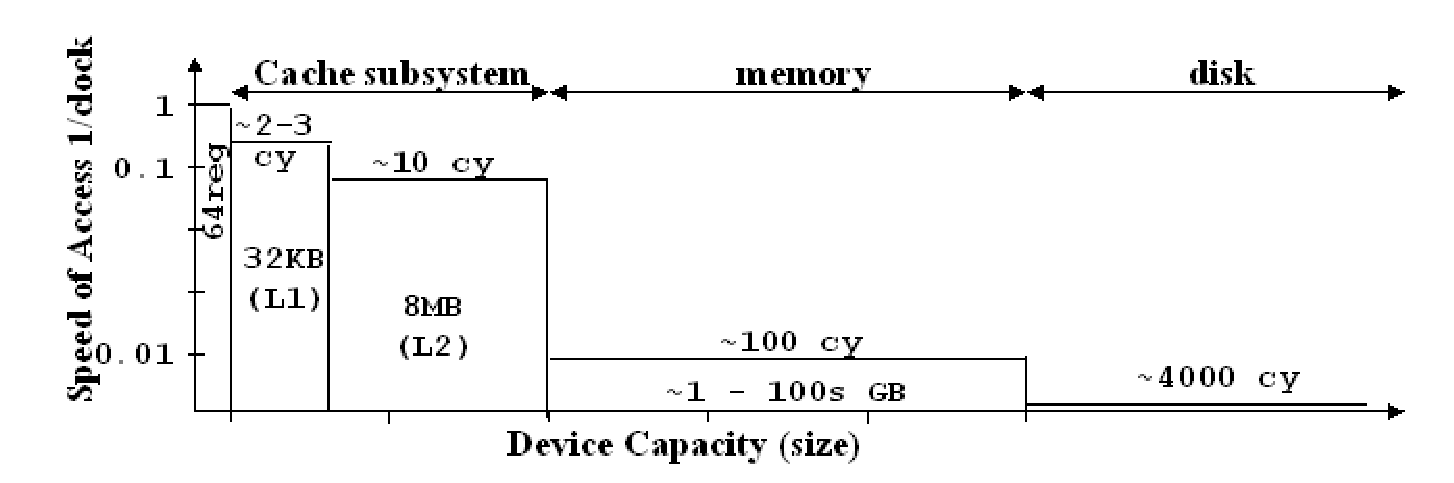
\includegraphics[height=4cm,
    angle=0]{./images/memory_latency.eps}}
  \caption{Hierarchy of memory in CPU with memory latencies}
  \label{fig:memory_latency}
\end{figure}

Another important example is the balance between using
\begin{enumerate}
\item amount of shared memory per block (e.g. 4KB)
\item number of threads per block (e.g. 256)
\item number of registers per thread (e.g. 10)
\end{enumerate}

{\bf Example}: Suppose in Tesla 1 (GF8800), an SM can accommodate
maximum 8 blocks at a time. With 16KB shared memory per SM, based on
the amount of shared memory use {\it per se}, there is maximum 4
active blocks. Based on the number of threads per block, with 4 active
blocks, the number of active threads is $4\times 256 = 1024$ which
pass the limits of Tesla 1 (i.e. 768 threads). What if 3 active
blocks, then the number of active threads is $3\times 256 = 768$ which
is OK. So, the first two information limits the number of active
blocks to 3. How about the third information, with 10 registers per
thread, the number of registers using is $10\times 768=7680$ which is
still smaller than the current available 8192 registers per SM.

Now, suppose that some how in our implementation we increase one
register, i.e. each thread use 11 registers. Then, the number of
registers used by 768 active threads is $11\times 768 = 8448$ which
pass the limit. This forces CUDA to have only 2 active blocks per SM
(or 512 active threads per SM). As you can see, this dramatically
decreases the number of active threads to 33\%. 

However, if we increase the shared memory an amount of 1KB per block
(i.e. 25\% increase in share memory usage), the number of shared
memory use is $5\times 3 = 15$ still smaller than 16KB, which means it
doesn't change the number of active blocks or the performance of the
system doesn't decrease, but can be increased (due to higher
locality).

\begin{enumerate}
\item Ensure executing threads are not starved for data
  \begin{itemize}
  \item avoid global memory bandwidth is the bottleneck
  \item balance high utilization (i.e. warps are always available for
    execution while some are stalled on high-latency operations
    $\rightarrow$ increase more active threads in a SM) and efficient
    instruction stream (i.e. using fewer instructions while can
    increase the sequences of independent instructions within a
    warp). 
  \end{itemize}
\end{enumerate}

Since Fermi, true caches are available. However, knowing how to
maximize cache line utilization is important
(Sect.~\ref{sec:shared-memory-cache}). 

\begin{framed}
  Here are some information from CPU that may provide a roughly
  information how cache hit and cache miss affect to the performance
  \begin{enumerate}
  \item CPU registers : 0 cycles
  \item L1 cache hit: 2-3 cycles
  \item L1 cache miss, L2 cache hit: 8-10 cycles
  \item L2 cache miss, no TLB miss : 75-250 cycles
  \item TLB missing and require re-load of TLB: 2000 cycles
  \item TLB missing and require load of virtual page from disk:
    hundreds of millions of cycles
  \end{enumerate}
\end{framed}

\begin{framed}
  A cache hit load the word from the cache line. A cache miss for a
  single data element requires loading the whole cache line from
  memory.
\end{framed}

Another important issue is array indexing, which may affect loop nest
optimization (LNO)\footnote{LNO is enabled if we use -O3
  compiler flag, or we can turn on using -LNO option}. The
array should be accessed in a most natural way (i.e. direct indexing), Fig.~\ref{fig:array_index}.

\begin{framed}
  Techniques in LNO
  \begin{itemize}
  \item loop interchange
  \item loop unrolling
  \item loop blocking for cache
  \item loop fusion
  \item loop fission 
  \item  pre-fetching
  \end{itemize}
\end{framed}

\begin{figure}[hbt]
  \centerline{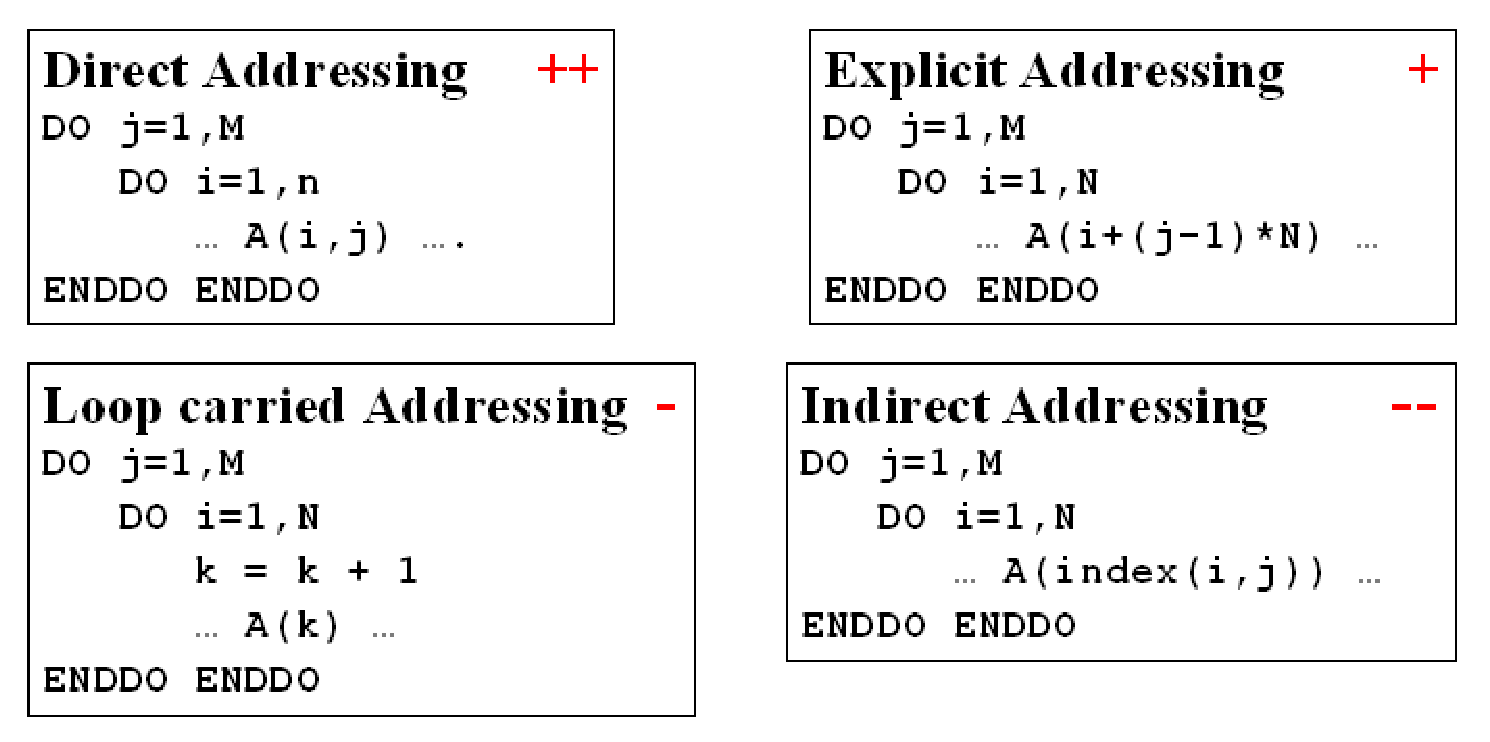
\includegraphics[height=5cm,
    angle=0]{./images/array_indexing.eps}}
  \caption{(+) is preference, (-) should be avoided as the compiler
    don't know how to perform LNO}
  \label{fig:array_index}
\end{figure}


\begin{figure}[hbt]
  \centerline{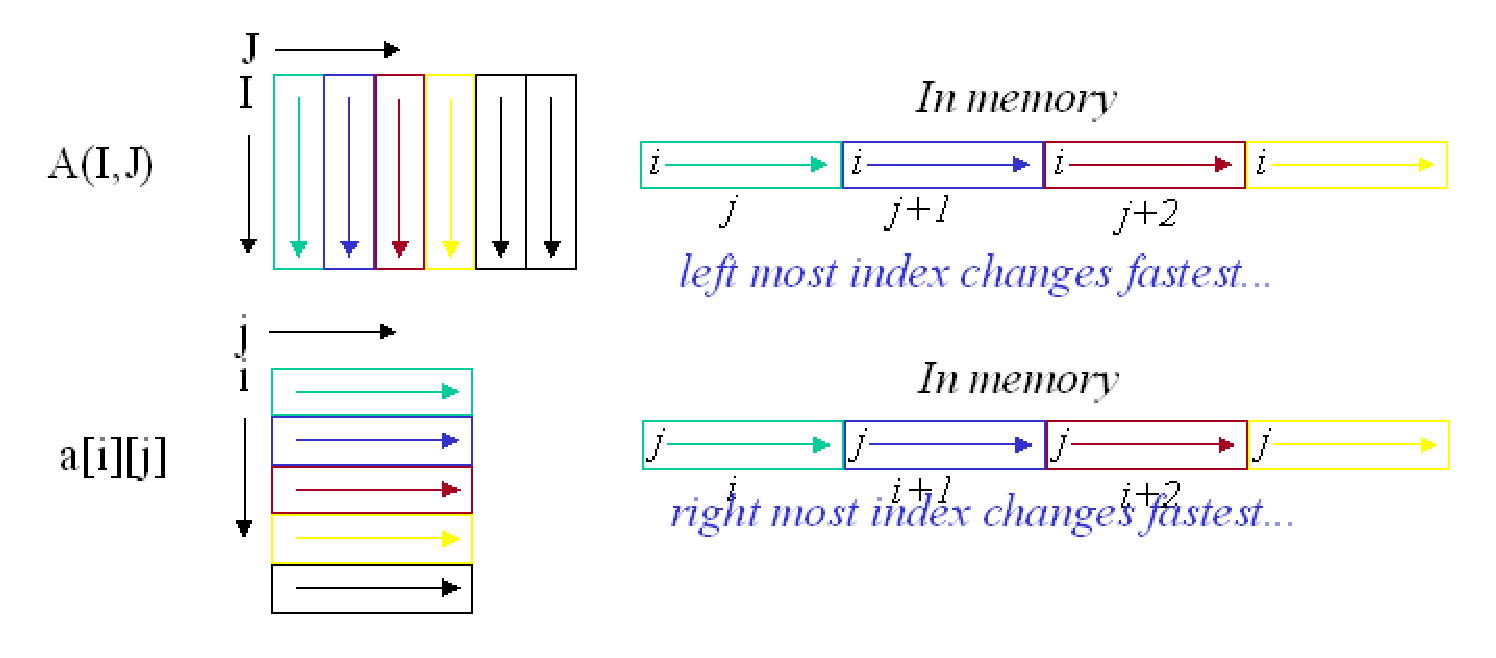
\includegraphics[height=5cm,
    angle=0]{./images/memory_layout.eps}}
  \caption{Memory layout in Fortran (column-major) and C (row-major)}
  \label{fig:memory_layout}
\end{figure}

Another important issue is to access array elements in storage orders,
Fig.~\ref{fig:memory_layout}. So for column-major arrays in Fortran,
put the index of the slowest changing (i.e. row) as the outer most
loop. However, in the case of matrix multiplication, we have two
options: (1) good index for B and bad for A, C; (2) bad index for B
and good for A, C. We cannot achieve good index for all; so we have to
choose the second one, Fig.~\ref{fig:index_matrix_mul}. We call this
{\bf index reversal}. 

\begin{figure}[hbt]
  \centerline{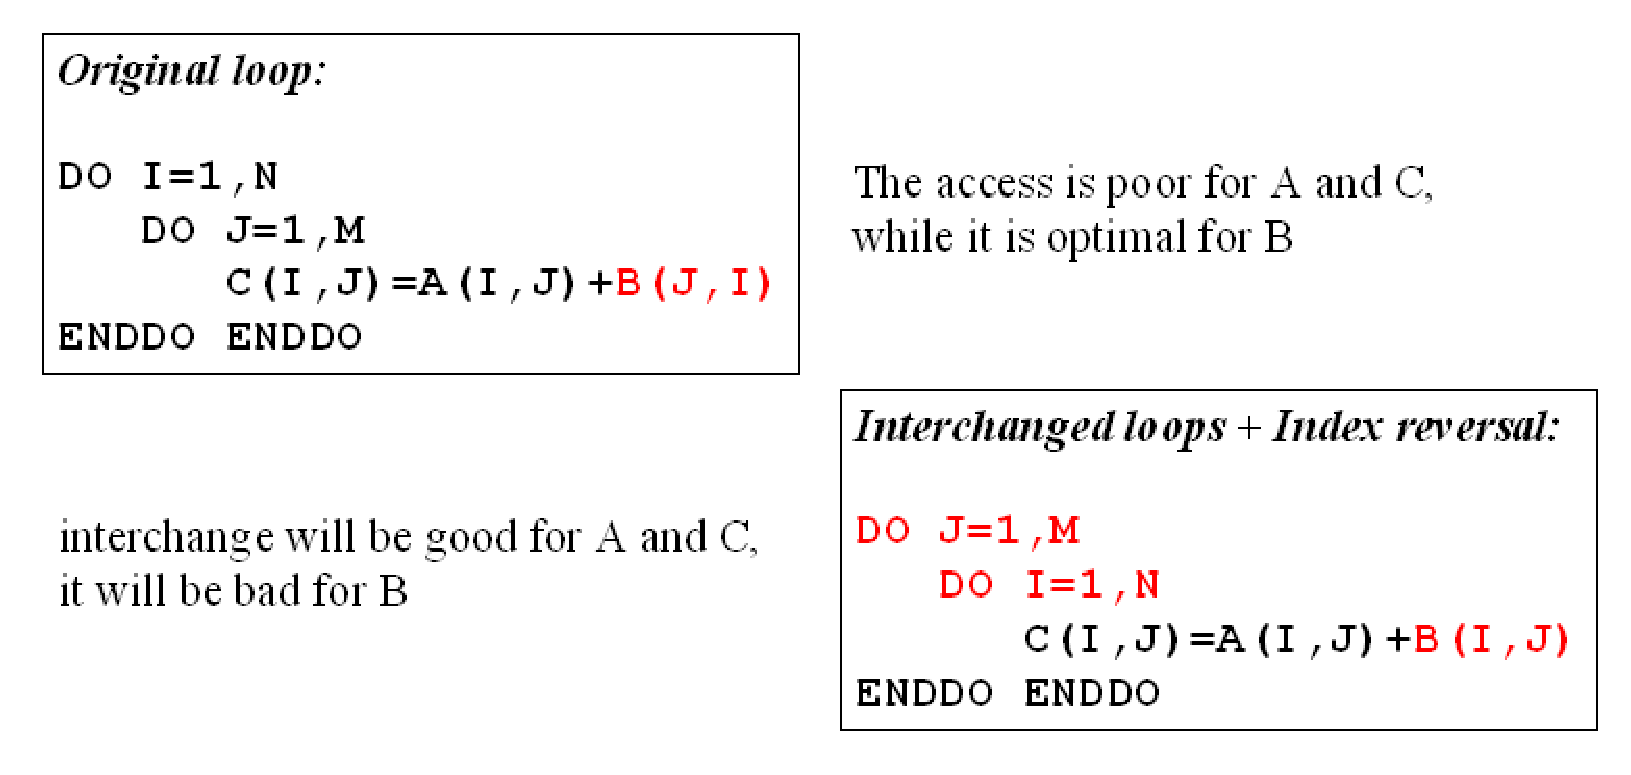
\includegraphics[height=5cm,
    angle=0]{./images/index_matrix_mul.eps}}
  \caption{Index reversal effect}
  \label{fig:index_matrix_mul}
\end{figure}

Choosing a right looping order affect the execution time a lot,
Fig.~\ref{fig:loop_interchange} .
\begin{figure}[hbt]
  \centerline{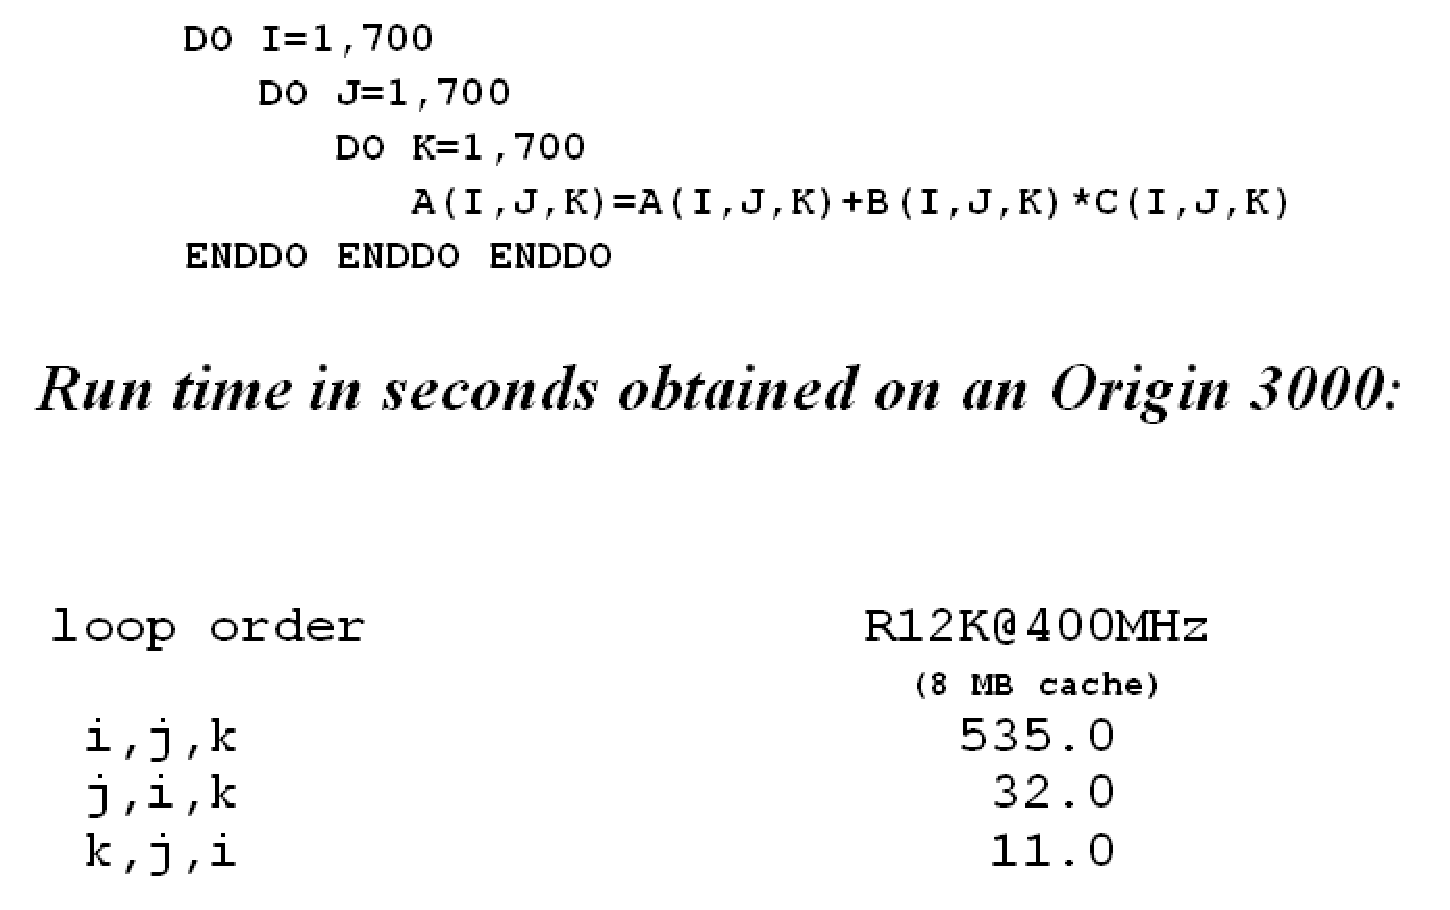
\includegraphics[height=5cm,
    angle=0]{./images/loop_interchange.eps}}
  \caption{Loop interchange in Fortran}
  \label{fig:loop_interchange}
\end{figure}



Here are some basic tips:

\begin{enumerate}
\item * Make sure global memory reads and writes are coalesced where
  possible (see programming guide section 6.1.2.1).

\item * If your memory reads are hard to coalesce, try using 1D
  texture fetches (tex1Dfetch) instead.
\item * Make as much use of shared memory as possible (it is much
  faster than global memory).
\item  * Avoid large-scale bank conflicts in shared memory.
\item * Use types like \verb!float4! to load 128 bits in a single
  load.

  The primitive \verb!float4! can pack 4 floating-point number
  efficiently.  Using float4 (instead of float3) data allows coalesced
  memory access to the arrays of data in device memory, resulting in
  efficient memory requests and transfers.

  An array of 6 float4 types then holds one lattice size of the quark
  field.

\item  * Avoid divergent branches within a warp where possible.
\end{enumerate}


\textcolor{red}{We recommend using the CUDA Visual Profiler to profile
  your application} (Chap.~\ref{chap:profiling-tool}).

\section{Data types}
\label{sec:data-types}

\subsection{In C/C++}
\label{sec:cc++}


CUDA support 
\begin{enumerate}
\item built-in vector types in C. 
\item char1, char2, char3, char4
\item uchar1, uchar2, uchar3, uchar4
\item short1, short2, short3, short4
\item ushort1, ushort2, ushort3, ushort4
\item int1, int2, int3, int4
\item uint1 , uint2, uint3, uint4
\item long1, long2, long3, long4,
\item ulong1, ulong2, ulong3, ulong4,
\item float1, float2, float3, float4
\item doubles :
  \textcolor{red}{available in GPU with CC. 1.3 or above}
\item \textcolor{red}{constructor of the form} \verb!make_<typename>!,
  e.g. \verb!make_int2()!
\begin{lstlisting}
int2 x = make_int2(int x, int y);
\end{lstlisting}
\end{enumerate}
Data with the above data type are linearly allocated on physical
memory, regardless of their high dimension logical definition. GPU has
a special memory space in that data are physically organized in 2D or
3D. 
\verb!cudaArray! is a special data type 

\subsection{In Fortran}
\label{sec:fortran}

Fortran interoperability types with C can be used. This is specified
in the .... module. In addition, we can also use Fortran intrinsic
types like
\begin{itemize}
\item INTEGER
\item REAL
\item DOUBLE PRECISION
\item KIND data type
\end{itemize}

\subsection{Type casting (mapping)}
\label{sec:type-casting-mapping}

\begin{enumerate}
\item Type conversion
\begin{lstlisting}
 unsigned int __float2uint_[rn,rz,ru,rd](float);
 float __int2float_[rn,rz,ru,rd](int);
 float __uint2float_[rn,rz,ru,rd](unsigned int);
\end{lstlisting}

\item Type casting
\begin{lstlisting}
 float __int_as_float(int);
 int __float_as_int(float);
\end{lstlisting}
\end{enumerate}

\subsection{Special instructions}
\label{sec:special-instructions}

{\bf Special instructions}:
\begin{enumerate}
\item Boolean, shift, move, compare, convert, bitfield extract,
  bit-reverse insert, and population count.
\item Single-precision floating-point transcendental
  instructions\footnote{NOTE: Transcendental functions are functions
    that are not in polynomial forms, e.g. sine, cosine, exponential,
    rational function, square root},
  e.g. sine, cosine, reciprocal, and square root (NOTE: no support for
  double-precision)
  \begin{itemize}
  \item Tesla 1st + 2nd gen: executed by 2 SFU (special functional units)
  \item Fermi: executed by 4 SFU, each execute 1 instruction per
    thread, per clock. Thus, with 32 threads, a warp need 8 clocks to
    execute a transcendental operation.
  \end{itemize}

\item Atomic functions
  \begin{itemize}
  \item Tesla 1st gen: not available
  \item Tesla 2nd gen: support, yet double precision only work on
    global device memory. 
  \item Fermi: 20x faster (with L2 cache), and allow double precision
    data to reside on L1/shared or L2 cache memory. 
  \end{itemize}
\end{enumerate}q
Atomic functions: Performs a read-modify-write operation on one 32 bit
word residing in global memory, e.g. 
\begin{lstlisting}
unsigned int atomicAdd(unsigned int* address, unsigned int val);
\end{lstlisting}
At present limited support for integer types only!

\section{Memory access}
\label{sec:memory-access}

There are 2 main types of memory:
\begin{enumerate}
  \item DRAM (Dynamic RAM): high densities, and cheaper cost/bits. So, DRAM is
  used as main memory. DRAM is long latency, leaky (as data is stored in
  capacitor and capacitor leak charge, thus information fades away and thus
  the capacitor need to be refreshed periodically). This makes DRAM dynamic, not
  like SRAM. 
  \item SRAM (Static RAM): lower densities (1/4 to 1/8 of DRAM), yet higher
  speed (8-6x faster); also it costs more per bit (8-16x higher). So, SRAM is
  optimized for speed (e.g. caches)
\end{enumerate}

As DRAM is used for main memory, we will describe more about DRAM.
To understand how memory is accessed, first we need to know how memory
chips (DRAM) are
organized
and
addressed\footnote{\url{http://www.pcguide.com/ref/ram/timingAccess-c.html}}.
{\bf Memory chip} is stored as a matrix (rectangular arrays) with rows and
columns are called {\bf wordlines} and {\bf bitlines}, respectively.

\begin{figure}[hbt]
  \centerline{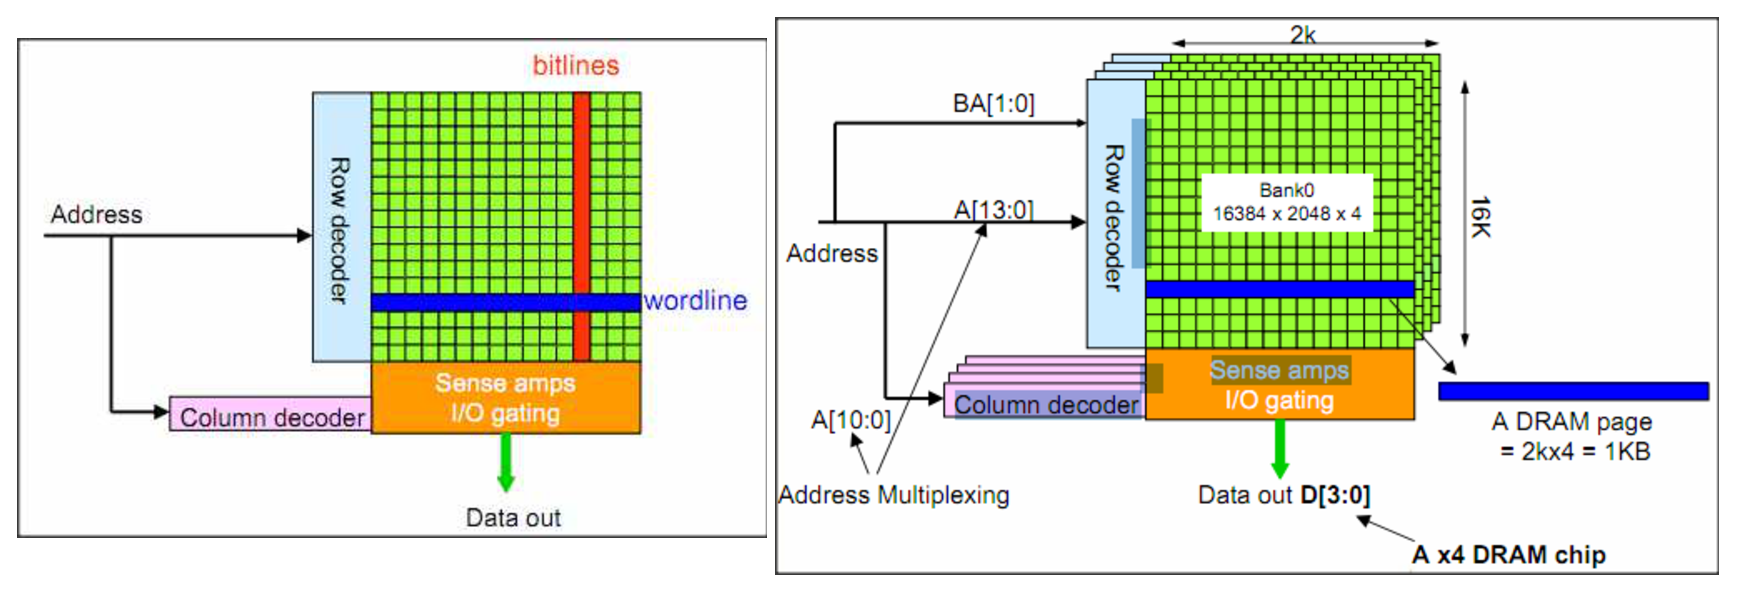
\includegraphics[height=5cm,
    angle=0]{./images/DRAM_architecture.eps}}
  \caption{DRAM architecture, (B) 512 MB 4-bank DRAM }
  \label{fig:DRAM}
\end{figure}

SRAM requires 6 transitors; while each bit of DRAM needs only 1 transitor and
1 capacitor. Thus billions of transitors can fit on a single memory chip. An
element in DRAM is a bit line (information), a wordline (control: read or write?), and a storage capacitor. An array of DRAM has a number of bitline (0..15) and a number of wordline (0..1023). DRAM is organized in multi-banks
chip. Each core array (memory chip), Fig.\ref{fig:DRAM}, has about 1M bits, with
\begin{enumerate}
  \item a sense amplifier: amplify the signal (or charge) detected on a memory
  cell
  \item address logic: to select row/column
  \item RAS (Row Address Select), and CAS (Column Address Select) logic latch:
  resolve the row/column addresses (initiate and terminate read/write
  operations). 
  \item internal counters (or registers): to keep track when/where to refresh
  \item output enable logic: to prevent data from appearing in the output unless
  specifically desired.
\end{enumerate}

\begin{framed}
As DRAM memory is leaky, charge need to be restored, i.e. to be refresh
periodically. The frequency for refreshing depends upon the silicon technology
used for the chip and design of the memory cell itself. Reading/Writing have
the effect of refreshing also. Normally, DRAMs are refreshed one row at a
time. The data is unaccessible when refreshing. There are 3 refresh policies:
Row Address Strobe only refresh (ROR) and CAS-before-RAS (CBR) and hidden refresh.
\end{framed}

RAS is active low, i.e. it must be at low Voltage to active. In a
complete memory cycle, $t_{RAS}$ is the minimum time that RAS must be active,
and $t_{RP}$ is the minimum time that RAS must be inactive. RAS can be used to
trigger a refresh cycle (RAS-only refresh (ROR)). CAS can be used to initiate a
read/write operation, or trigger a refresh cycle (CAS-before-RAS refresh) which
require CAS to be active before RAS and remain active during that time.
$t_{CAS}$ is the minumum time that CAS must remain active, and $t_{CP}$ is the
minimum time that CAS must remain inactive (CAS precharged time). 

Suppose that the memory chip
is addressed by 22 bits, then the lower-order 11 bits are considered
the ``row'', and the higher-order 11 bits are the ``columns''. As a
result, we only need an address-bus of 11 bit length only. This is known as {\bf multiplexing}.
{\it Why don't we use total 22 bits and organized as a array?}  - The
main reason is ``cost''.

\begin{framed}
  Even though memory chips are addressed in row/column manner, memory
  address are single numbers, not in pairs or triple\ldots There is no such
  thing as two dimensional memory. So, higher dimensional arrays are logically
  mapped to scalar-indices by the compilers. How a 2D index is mapped to 1D
  index in memory is determined by the compiler. Fortran do
  this column-by-column; while C/C++ does this row-by-row.
\end{framed}

A DRAM memory doesn't have a single memory chip, but dozens of them in which
chips are arranged into {\it modules}, and then into {\it banks}. The
{\bf memory controller} manages which set of chips are read from or
written to. 



The amount of time from the moment the memory controller
tell the address until the valid data is retrieved and is available is
called the memory's {\bf column-address strobe (CAS)} latency or
access time, $t_{AC}$ (ns). The lower the CAS latency, the better.

SDRAM allows more complex pattern of memory access.  In
asynchronous SDRAM, the interval is specified in nanoseconds and is
constant, e.g.  today memory access range from 5-70ns in which the
time between supplying a column address and the receiving of
corresponding data is 10-15 (ns).  However, in SDRAM, the interval is
dependent upon the number of clock ticks and varies upon the clock
rate. So, the interval in SDRAM is specified in clock cycles
(\textcolor{red}{this is the unit we use in GPU to measure the
  delay}). {\bf We will focus on SDRAM only}.

\begin{framed}
  Original SDRAM is single-data rate. Latest generations of SDRAM are
  double-data rate (DDR). Currently, 184-pin DDR SDRAM is widely used
  as a standard. Now, we have DDR2, DDR3 and (to be released in 2012)
  DDR4.
\end{framed}

The initial access to memory normally take more times than subsequent
memory access - \textcolor{red}{about 4 to 7 clock cycles}, as there
are certain signals that have to be set to begin the access. Next, the
row address is sent, followed by column address. The memory controller
will read the data from the cell of that address, and transfer it
back.  Normally, when you read the data at position $i$, it's likely
that you will read data at adjacent addresses in the range $i\pm j$ as
well (with $j$ is a small interval). So, in microprocessor design, to
enhance the performance, data from a single row buffer are read in
chunks, e.g. 8-dataword rather than a single dataword. This is called
{\bf burst mode access} or {\bf bursting}.

\begin{framed}
  DDR has a {\bf prefetch buffer} that allows access to more than one
  dataword residing on a physical row in the memory. This is known as
  {\bf burst mode access} (or bursting).
  \begin{itemize}
  \item In SDRAM : only one word is transmitted per clock cycle
  \item In DDR1 SDRAM: read/write at least 2 consecutive words per
    clock cycle
  \item In DDR2 SDRAM: read/write at least 4 consecutive words per
    clock cycle.
  \item In DDR3 SDRAM: read/write at least 8 consecutive words per
    clock cycle (i.e. 8n prefetch architecture)
  \end{itemize}
  So, it's best to have your program organized in such a way that data
  in consecutive memory addresses are read/write at once.
  Normally, data is read/written in a chunk of size equal to the
  {\bf cache line} which can be 32-byte, 64-byte, or 128-byte depending
  on cache level (read Sect.~\ref{sec:cache-review}).
\end{framed}


\begin{figure}[hbt]
  \centerline{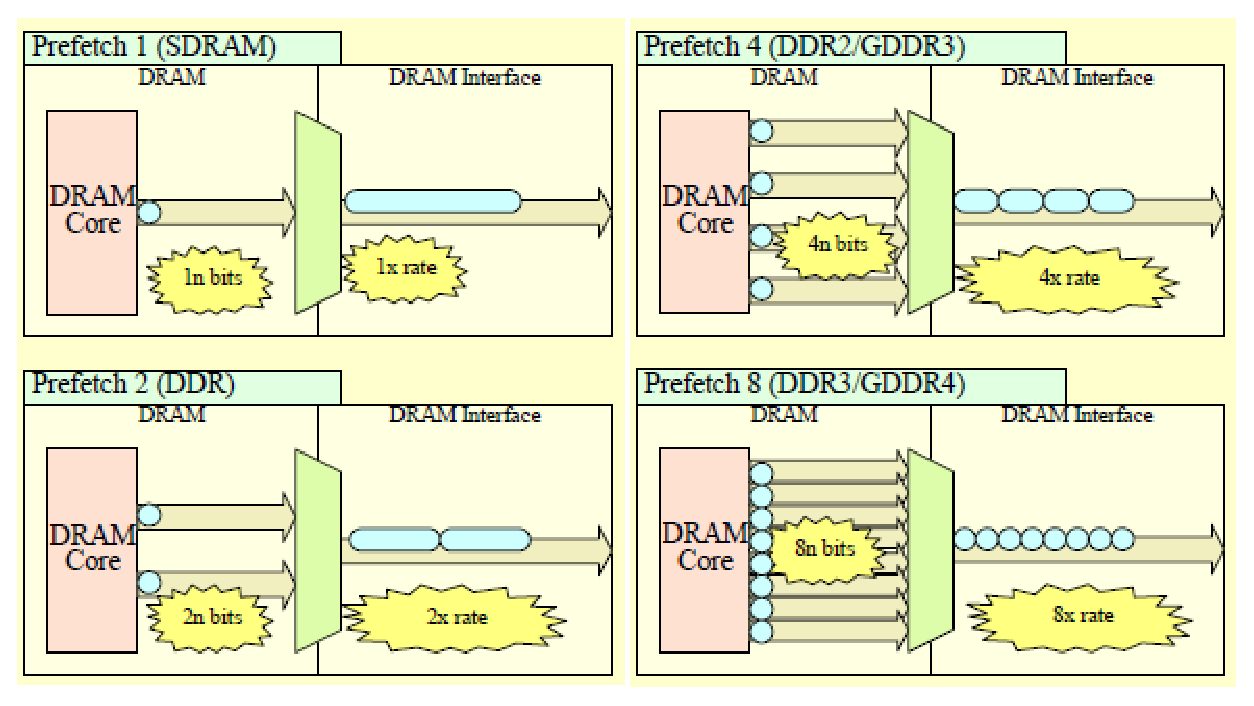
\includegraphics[height=5cm,
    angle=0]{./images/DRAM_access.eps}}
  \caption{SDRAM memory access}
  \label{fig:SDRAM}
\end{figure}

Reading a cell in
a core is very slow.
\begin{enumerate}
  \item DDR: core speed = 1/2 interface speed
  \item DDR2/GDDR3: core speed = 1/4 interface speed
  \item DDR3/GDDR4: core speed = 1/8 interface speed
  \item \ldots (it seems that interface speed increase faster than core speed)
\end{enumerate}
Thus to improve the performance, memory access should be perform in bursting using internal
  buffer. 
So, the core speed in nVidia GTX280 is 276MHz, while the GDDR3 interface speed
is 1.1GHz (64-bit interface). So, it can sustain about 17.6GB/s. How can we
reach theoretical global memory peak of 141.7GB/s. This can be done by using
multiple memory channels. So the hierachical structure is:
\begin{itemize}
  \item multiple channels
  \item each channel has multiple banks
  \item each banks has a core memory
\end{itemize}
So, to tell where the data reside, some bits tell the channel, some others tell
the DRAM bank; and finally some determines the position for bursting access.    
In nVidia GTX280, every 30 Streaming-Processors get access their own 8-channel DRAM controllers. 

DRAM bursting always return a bunk of bits, eventhough the data required is
smaller than that. In a multi-bank DRAM, bursting death time (i.e. cannot
read/write to the same bank at a certain time period) can also be hidden further
when we perform read/write to another bank on the same chip.

So, it's highly efficient when accessing data on the same chip, and on the
same bank. There are different situation that can degrade the performance, when
(1) the data is on the same chip, but not on the same bank, (2) the data is not
o the same chip. There are 3 types of DRAM: Asynchronous DRAM, Synchronous DRAM
(SDRAM), and RDRAM. 

% Thus, the latency for the second/third/fourth chunk is now
% \textcolor{red}{1-3 clock cycles}.  With 4 chunks in a group, the
% access time is given in the form of $x-y-y-y$, with $x$ is the time
% for the first chunk, $y$ is the time for the second, third and fourth
% chunks.  For example: using burst mode, SDRAM is at best 5-1-1-1, and
% cache is 3-1-1-1.

\begin{framed}
  DDR3 SDRAM run at 1.5V. The future DDR4 SDRAM is supposed to run at
  1.2V or less. 
\end{framed}

DDR memory in GPU is SDRAM and is a little bit different in naming,
i.e. graphics DDR synchronous graphics RAM (GDDR SGRAM). GT200 use
GDDR3 SGRAM - a DDR2-based memory. Fermi use GDDR5 which is based on
DDR3.
\textcolor{red}{GDDR5 interface transfer two 32-bit wide words per
  write clock (WCK)}
cycle. A single read/write access consists of 256-bit wide two-CK
cycle data transfer, i.e. as it can do read/write at the same time we
have 2 x (2CK) x (2 32-bit) = eight 32-bit = 256-bit.
\begin{itemize}
\item CK = the clock rate when do read/write (e.g. 1.25GHz)
\item WCK = the clock rate when do read only (e.g. 2.5 GHz)
\end{itemize}
% Thus, a single read/write, with 384-bit wide, it can transfer 6
% double-precision words or 12 single-precision words using 2 clock
% cycles at the internal memory core and 8 WCKs.


\subsection{DRAM in GPU}
\label{sec:dram-gpu}

Memory system is very parallel. To take advantage of that, we need to
have many parallel memory operations, by running many parallel
threads, each doing some memory access.

As memory are accessed in a chunk of bytes, by giving the starting
address and it will return a number of bytes (typically 64byte or
128bytes; even you only need 4byte), known as bursting memory
access. Thus, memory accesses from a warp can nicely utilize DRAM
bursts if they are coalesced, i.e. in adjacent location.

For access across warps, the steering bitfields, which is used to
decode channel/banks, should be as {\bf distinct} as possible,
i.e. two warps should access memory from different memory banks. This
will increase parallelism as memory access at a single bank is still
sequential. QUESTION: How can we control the data should be on
different memory bank? - ANSWER: Thanks to interleaved memory access,
the dynamic set of simultaneously active thread blocks to access
different memory banks need a good dynamic block scheduling policy:
{\it two blocks with near blockIdx.x will access memory closed to each
  other};
and otherwise. So based on this heuristic rule, data are organized
\begin{verbatim}
block1  block2  ..... blockn

bank1   bank2         bankk
       (block2)       (block1)
       (blockn)
\end{verbatim}
Here, 2 distant thread blocks (n and 2) access data assigned in the
same memory bank; while 2 adjacent thread blocks will be designed to
access data on 2 different memory bank.


Example: the least significant bits tell which channel, which banks
and then which words to access.

Threads 0-7 globally all access the data on 2 channels: 0 and 1. The
important is the patterns: they are nicely coalesced. 


Example: stride access, i.e. add every 4 elements A[4*i] = A[4*i] +
B[4*i]. There are dead empty space, as the data now reside on
different channels and different banks, so it takes more memory
accesses. In addition, at each channel, we don't utilize all banks,
i.e. wasting memory bandwidth. 


Example: each block process a tile of data, and each one skip a tile
of data. E.g.: block 1 accesss data from 0-3, block 2 acecss data from
8-11. Here, block 1 utilize data on same channels and utilize all
banks. And similar for block 2 which use channel 2. However, even
though we utilize all banks in a channel, we never utilize all the
channels. In other words, channel 1, 3, ... are never used. This is
another form of waste. 


Example: striding in multidimensional arrays. NOTE: memory is linear,
and multidimensional array is just a logical organization for
programmer convenient by the programming language. In the end, they
need to be mapped to linear arrangement. 

In C, each thread need to access data in a single column. This will
guarantee threads in a block access data on the same row, which are
at adjacent locations on memory. 

\begin{framed}
  Striding may not be a big issue in Fermi, for applications like
  atom, and use float4. But for fluid dynamics application or using
  float8, it still an issue. (NUMBERS MATTER).
\end{framed}

What is an array element is a data structure. This is another problem
we need to notice? - Use a structure of multiple arrays of data
element rather than using a single array of data structure of multiple
data elements. In other words, change arrangement of data to better
match thread access pattern, i.e. AoS (array of structure) vs. SoA
(structure of array). Two ways to resolve
\begin{enumerate}
\item transpose: take 2 dimension and just transpose them
\begin{verbatim}
X0,0  ...
X0,1  ...
X0,2  ...
X0,3  ...
\end{verbatim}
become
\begin{verbatim}
X0,0  X0,1  X0,2  X0,3
  ..........
  ........
  .........
\end{verbatim}

\item tile: take a single array dimension and split into 2 dimension,
  i.e. change a stride access pattern into a contiguous
  access pattern in some dimension. So, old A[i] becomes A[i/N][i\%N]
\begin{verbatim}
A0 .... A4 ... A8 ... A12
\end{verbatim}
  becomes
\begin{verbatim}
A0,0 ...
A1,0 ...
A2,0 ...
A3,0 ...
\end{verbatim}

\end{enumerate}
Using {\bf tile}, we don't move any data; but with {\bf transpose}, we
really move the data. Depending on your data structure and access
pattern, you can choose a right one to use. Aos vs. SoA is a special
case of transpose. SoA is about 4X faster than AoS on GTX280. 


\begin{framed}
  There are some software tools that automatically transform your AoS
  to SoA. 
\end{framed}

Array padding is commonly used to guarantee the starting address of
each row (in C) (or column in Fortran) is aligned, i.e. a multiple of
64 or 128, depending on GPU generation. Alignment is not a performance
cliff in Fermi, as long as you're going to access those data soon as
they are stored in the cache. 


There's a tool from OpenCL can be used




\subsection{Memory Padding}

The CPU can access data with less memory fetching when the data is aligned
\begin{itemize}
  \item all 4-byte variables must line up on boundaries divisible by 4
  \item all 2-byte variables must line up on boundaries divisible by 2
  \item all 1-byte variables must line up on boundaries divisible by 1 (so not
  a problem)
\end{itemize}
Data alignment is very important, especially in embedded systems. The call
\verb!malloc()! doesn't allocate a variable at a given size at any memory
address, but following certain rules.

The reason it's important is that data are read in work-sized chunks (e.g.
4-byte chunk in a 32-bit system, and ???-byte chunk in a 64-bit system). So, by
putting the data at a memory offset equal to some multiple of the word size, we
call it {\bf data alignment}. For a given data structure, it may be necessary to
insert some meaningless in the end the data structure and at the front of the
next data structure. This is known as {\bf data structure padding}. 

So, it's depending on how the structure is organized, the computer may use more
or the same number of bytes for an allocation. Example: a structure with 4 data
element, each one with a certain size, following the order: 
\begin{verbatim}
1 4 1 2  vs.   4 2 1 1
\end{verbatim}
In the first case, the computer uses: 1 + 3 padding + 4 + 1 + 1 padding + 2 = 12
bytes (4 bytes of padding). In the second case, no padding is required, so it
needs only 8 bytes.
\begin{lstlisting}
struct pt{
  int i;
  byte j;
  char k;
  char l;
}
\end{lstlisting}

To enforce the memory of a struct begins at an address in memory that is a
multiple of $n$ bytes, then we use \verb!__align(n)__!. If the size of the
struct is not a multiple of $n$ bytes, then padding is inserted to ensure the
struct is properly aligned. 

How to use in CUDA C
\begin{lstlisting}
#if defined(__CUDACC__) // NVCC
   #define MY_ALIGN(n) __align__(n)
#elif defined(__GNUC__) // GCC
  #define MY_ALIGN(n) __attribute__((aligned(n)))
#elif defined(_MSC_VER) // MSVC
  #define MY_ALIGN(n) __declspec(align(n))
#else
  #error "Please provide a definition for MY_ALIGN macro for your host compiler!"
#endif
\end{lstlisting}
and then we can use
\begin{lstlisting}
struct MY_ALIGN(16) pt { int i, j, k; }
\end{lstlisting}

\begin{framed}
To choose a proper value for $n$, we want to mimimize the amount of padding
required. From the CUDA programming guide, the hardware requires each thread
reads words aligned to 1,2,4, 8 or 16 bytes.
\end{framed}

Example: If we use
\begin{lstlisting}
struct MY_ALIGN(16) {
  int a;
  int b;
  int c;
  int d;
  float* el;    
};
\end{lstlisting}
On a 32-bit system, a pointer take 4-byte, so totally, the struct takes 20
bytes. So, using 16-byte alignment will waste 
\begin{verbatim}
16 * (ceil(20/16) - 1) = 12    (bytes)
\end{verbatim}
per struct. On a 64-bit system, a pointer is 8-byte, so totally, the struct
takes 24-bytes, i.e. it waste 8-bytes per struct. To reduce the waste, we can
use \verb!MY_ALIGN(8)!. The trade-off is that the hardware need to use three
8-byte loads, instead of two 16-byte loads to load a struct from memory. [NOTE:
We don't want to align smaller than 4-byte]. If memory is an issue, then we
probably use \verb!MY_ALIGN(8)!. If memory load is a bottleneck, then we
probably use \verb!MY_ALIGN(16)!. 


Example: Let's see another
example:\url{http://stackoverflow.com/questions/12778949/cuda-memory-alignment}
\begin{verbatim}
struct MY_ALIGN(16) {
  int a;
  int b
  int c
  int d
  float* i;
  float* j;
  float* k;
};
\end{verbatim}

For multi-dimensional array, multi-dimensional arrays can also be allocated
using the CUDA API interfaces to cudaMallocPitch and cudaMalloc3D. These
interfaces pad the array leading dimension to maximize aligned memory references
on the device. PGI's implementation of ALLOCATE in Fortran will never pad the
arrays; we've generally associated ALLOCATABLE arrays with contiguous memory.
Plus, Fortran programmers have been adding their own padding to arrays for
years; if that is your intent, you know how to do it. Reference:
\url{http://www.pgroup.com/lit/articles/insider/v2n1a3.htm}


\subsection{Data memory on GPU}
\label{sec:data-memory-gpu}

There are different kinds of memory spaces on GPU. 
\begin{itemize}
\item Register - dedicated HW - zero cycle
  (Sect.~\ref{sec:register-memory})
\item Shared Memory - dedicated HW - single cycle
  (Sect.~\ref{sec:shared-memory-bank})
\item Constant Memory - DRAM, cached in C-cache, 1\ldots 10s\ldots 100s of cycles,
  - depends on cache locality (Sect.~\ref{sec:constant-memory})
\item Texture Memory - DRAM, cached in L1 texture cache, 1\ldots 10s\ldots 100s of
  cycles - depends on cache locality (Sect.~\ref{sec:texture-memory})
\item Instruction Memory (invisible to programmers) - DRAM, cached in
  I-cache
\item Local Memory - DRAM, no cache - *slow*
\item Global Memory - DRAM, no cache - *slow*
  (Sect.~\ref{sec:global-memory}) 
\end{itemize}

\begin{framed}
  Even though device global memory, like CPU memory, is organized in
  1D. GPU has a special region of memory designed to work in 2D (and
  2D/3D in Fermi), i.e. there is no latency different when access any
  location in the 2D array in this memory space. This is known as
  {\bf texture memory}. Texture memory is specifically designed to
  render graphics images, so reading data in texture memory from
  kernel is read-only.
\end{framed}

In GT200, shared memory, global memory and texture memory have their
own memory space. Since Fermi, a unified memory space has been
developed where we can reference to data in either global memory
space, shared memory space or cache memory space; BUT NOT texture
memory, using a single pointer
(Sect.~\ref{sec:unified-memory-space}). However, the concept of using
pointer only work in C/C++, not in Fortran. 

CUDA threads are running in group in a SIMT manner. In CC1.x, data
access are performed in half-warp; while in CC2.x, data access are
performed in whole warp. It means that each thread in the group
doesn't have to make memory request separately if they access adjacent
memory locations. This is known as {\bf coalescing} and different
architecture requires different rules for coalescing memory
access. Coalescing memory access will save the time as one or two
memory is required for threads in the same groups (read
Sect.~\ref{sec:global-memory}).

In Fermi, the maximum: 144 GB/s peak off-chip memory access
bandwidth, which correspond to
\begin{itemize}
\item  36 G SPFP operands per second
\item  18 G DPFP operands per second
\end{itemize}
The speed of compute throughput is higher
\begin{itemize}
\item 1 TFLOPS SPFP peak throughput
\item 0.5 TFLOPS DPFP peak throughput
\end{itemize}
So, to achieve the maximum performance, a single data element
read-in from off-chip memory should be reused by as many arithmetic
operations as possible, before reading in a new one. The ratio of
\verb!#operations/data element! is 1,000/36 = $\sim$28 SPFP (14
DPFP) arithmetic operations to achieve best performance. 


\subsection{2D Linear memory }
\label{sec:linear-memory-}

\lstset{language={[90]Fortran}, numbers=left, numberstyle=\tiny,
  stepnumber = 5, numbersep=5pt, keywordstyle=\color{blue}}

As data are stored linearly at the physical level, it's best if data
is allocated in 1D. However, logically, working with multidimensional
data in its right dimension is easier. If you want higher performance,
you may want to know how to map from multidimensional indexing to the
correct offset location in the 1D array. 

\subsubsection{Fortran}
\label{sec:fortran-1}

We'll describe how to work in Fortran when column-major is used.

{\bf A(LBX:UBX, LBY:UBY)}.  

NOTE:
\begin{lstlisting}
ALLOCATE(A(LBX:UBX, LBY:UBY))
! is equivalent to
ALLOCATE(B((UBX-LBX+1) * (UBY-LBY+1))
\end{lstlisting}
we denote: 
\begin{verbatim}
MAXX = UBX-LBX+1, 
MAXY = UBY-LBY+1
\end{verbatim}
as the width for each dimension.  So A(x,y) can be accessed using B(i)
with
\begin{lstlisting}
i = MAXX * (y - LBY) + (x-LBX+1)
\end{lstlisting}


\textcolor{red}{Special case}: LBX = LBY = 1
\begin{lstlisting}
ALLOCATE(A(UBX, UBY))
! is equivalent to
ALLOCATE(B(UBX * UBY)
\end{lstlisting}
then
\begin{lstlisting}
i = MAXX * (y - 1) + x
\end{lstlisting}



\subsubsection{C/C++}
\label{sec:cc++-1}

\lstset{language={C}, numbers=left, numberstyle=\tiny,
  stepnumber = 5, numbersep=5pt, keywordstyle=\color{blue}}

\begin{lstlisting}
i = MAXY * (x - LBX) + (y-LBY+1)
\end{lstlisting}


\subsection{3D linear memory}
\label{sec:3d-linear-memory}

\lstset{language={[90]Fortran}, numbers=left, numberstyle=\tiny,
  stepnumber = 5, numbersep=5pt, keywordstyle=\color{blue}}

\subsubsection{Fortran}
\label{sec:fortran-2}

We'll describe how to work in Fortran when column-major is used.

{\bf A(LBX:UBX, LBY:UBY, LBZ:UBZ)}.  

NOTE:
\begin{lstlisting}
ALLOCATE(A(LBX:UBX, LBY:UBY, LBZ, UBZ))
! is equivalent to
ALLOCATE(B((UBX-LBX+1) * (UBY-LBY+1) * (UBZ-LBZ+1)
\end{lstlisting}
we denote: 
\begin{verbatim}
MAXX = UBX-LBX+1, 
MAXY = UBY-LBY + 1
MAXZ = UBZ-LBZ + 1
\end{verbatim}
as the width for each dimension.  So A(x,y, z) can be accessed using B(i)
with
\begin{enumerate}
\item Map A(x,y,z) to C(m,z), with
\begin{lstlisting}
m = MAXX * (y-LBY) + (x-LBX+1)
\end{lstlisting}
  and
\begin{lstlisting}
ALLOCATE(C(LBC:UBC, LBZ:UBZ)
! LBC  = 1
! UBC  = (MAXX * MAXY)
! MAXC = UBC - LBC + 1 = MAXX * MAXY
\end{lstlisting}

\item Map A(m, z) to B(i)
\begin{lstlisting}
i = MAXC * (z - LBZ) + m
  = MAXC * (z - LBZ) + MAXX * (y-LBY) + (x-LBX+1)
\end{lstlisting}

\end{enumerate}
Eventually, we have
\begin{lstlisting}
i   = MAXX*MAXY * (z - LBZ) + MAXX * (y-LBY) + (x-LBX+1)
\end{lstlisting}


\textcolor{red}{Special case}: LBX = LBY = LBZ = 1 
\begin{lstlisting}
ALLOCATE(A(UBX, UBY, UBZ))
! is equivalent to
ALLOCATE(B(UBX * UBY * UBZ)
\end{lstlisting}
then
\begin{lstlisting}
i   = MAXX*MAXY * (z - 1) + MAXX * (y-1) + x
\end{lstlisting}


\section{Memory fence}

Read also \ref{sec:memory-fences}

\url{https://www.google.com/search?q=_mm_sfence&aq=f&oq=_mm_sfence&aqs=chrome.0.57j62.279&sourceid=chrome&ie=UTF-8}

\url{http://stackoverflow.com/questions/4537753/when-should-i-use-mm-sfence-mm-lfence-and-mm-mfence}


\section{Device memory allocation}
\label{sec:device-memory-alloc}

Physically, memory are organized as linear memory address. And the only way
to work with device memory in C is to use pointer. So, the fatest way is to
map from higher dimension to 1D and allocate data as linear 1D array
(Sect.\ref{sec:linear-memory-alloc}). However, if you want to decare the
data as 2D or 3D, it's more efficient to pad data yourself to make sure each row
starts at an aligned address (i.e. 64-byte aligned). The reason is that
C (and hence C++) only really has 1D arrays - the C[i][j][k] arrays you're
describing are really arrays of pointers to other arrays of pointers, which in
turn point to the actual data. All that indirection (pointer-to-pointer) is bad
for performance. To pad data, CUDA C provides a convenient way to do this
using \verb!cudaMallocPitch()! (Sect.\ref{sec:pitched_lineararray}).

\begin{framed}
The pointer-to-pointer problem in C isn't an issue in Fortran (and I'm
guessing Matlab) because the Fortran language 'knows' what a multi-dimensional array is, and so can allocate a contiguous
block of memory and perform the index calculations itself.     
\end{framed}

If the 2D/3D data is specifically used for image/video processing and it needs
to be bind to texture, we should allocate the data using
\verb!cudaMallocArray()! (2D texture reference) and \verb!cudaMallocArray3D()! (ONLY 3D texture reference), and the
data is of \verb!cudaArray!
object\footnote{\url{http://forums.nvidia.com/index.php?showtopic=98408}}. To
make it work efficiently in texture, the organization of this data is not
normally, but z-curve, which is built to optimize for using texture where
contiguing local data is important. 

% 
% and to make it's
% easier for application that use 2D/3D logical organization of data,
% CUDA provide {\it CUDA array object} under the type \verb!cudaArray!. 

\begin{framed}
Linear memory exist on device in a 32-bit memory address space
  (Tesla 1, 2) and 40-bit memory address space (Fermi). So, we can use
  {\bf pointers} to reference to a linear memory object, which help
  building more complicated data structure, e.g. binary tree. 
\end{framed}

% \begin{framed}
%   Understand that memory, at the hardware level, is accessed in a
%   linear fashion; and multi-dimensional access is an illusion provided
%   by the compiler.
% \end{framed}
% If you have a 2D/3D array in host, and want to copy to device with cudaMemcpy(),
% each row (or in the case of Fortran, column) will be copied one by one in a
% loop. To make this faster, we either map 2D/3D to 1D linear before copy to GPU,
% or use \verb!cudaArray! object. CUDA provides some APIs to work with cudaArray
% object. 

\textcolor{blue}{CUDA array (cudaArray) object is an opaque memory layout
optimized for texture fetching} (Sect. 3.2.4 in CUDA C Programming Guide). This
works best if you plan to use  texture memory for (1) enhance performance for
accessing read-only data,  rather than reading directly from global memory, (2)
graphics output. 

Both 2D data declared with cudaMallocPitch() and 1D/2D/3D {\bf CUDA
array} can be bound to texture memory. {\bf When to use mallocPitch() vs. CUDA
array for texture ?} In 2D access, bound the texture to data allocated by
cudaMallocPitch() is faster than bound the texture to CUDA array.
% 
% \item In 2D or 3D, CUDA array help managing data better with
%   improved cache coherence when reading up/down columns as well as
%   across rows. For best performance, it's programmer's job to padd data to
%   match aligned size before allocation.


For allocations of 2D and 3D objects, it is highly recommended that programmers
perform allocations using cudaMalloc3D() or cudaMallocPitch(). Due to alignment
restrictions in the hardware, this is especially true if the application will be
performing memory copies involving 2D or 3D objects (whether linear memory or CUDA arrays).  

\subsection{Linear memory allocation}
\label{sec:linear-memory-alloc}

We use CUDA C runtime API \verb!cudaMalloc()! to allocate device memory, and
\verb!cudaFree()! to free memory.

In CUDA Fortran, we use \verb!allocate()! with variables having \verb!device!
attribute in CUDA Fortran


\subsection{Pitched linear array (cudaMallocPitch())}
\label{sec:pitched_lineararray}

The reason of using pitched linear memory is for data-coalescing. In CUDA C,
data elements in a 2D array is referenced using 2 pointers. So, it requires the
starting point of each row (or in CUDA Fortran, each column) to be aligned, i.e.
multiple of 32, 64 or 128 (typically 64). 

If we use 2D array, we have the option of padding the row/column manually; or
let CUDA do the job for us via \verb!cudaMallocPitch()!. \textcolor{red}{CUDA
Fortran doesn't need to use cudaMallocPitch()}. To copy an existing 2D array
to the pitched linear memory in device, we use \verb!cudaMemcpy2D()!, providing
it the pitch returned from the allocation cudaMallocPitch() funtion.
\textcolor{red}{``pitch'' is the width returned (in bytes) of the allocations}.
So, the number of bytes padded each row is equal to ``pitch - width''.


\begin{lstlisting}
cudaError_t cudaMallocPitch  (  void **   devPtr,
size_t *   pitch,
size_t   width,
size_t   height   
)  
\end{lstlisting}
The purpose of \verb!pitch! is to be used to compute the address within the 2D
array. Given the (i,j) as (row, col) location, its offset linear address is
\begin{verbatim}
T* pElement = (T*)((char*)BaseAddress + Row * pitch) + Column;
\end{verbatim}
with BaseAddress is the address of the initial bytes of the whole
    2D array, i.e. the object pointer. 
    In CUDA Fortran, as index start with 1, not zero, and it's
    column-major, we have
\begin{lstlisting}
T* pElement = (T*) ((char*) BaseAddress + 
                             (Column-1) * Pitch) + Row
\end{lstlisting}

\begin{framed}
The advantage of using cudaMallocPitch() is that data is copied faster, and
easier to
manage\footnote{\url{http://www.clear.rice.edu/comp422/resources/cuda/html/group__CUDART__MEMORY_g80d689bc903792f906e49be4a0b6d8db.html}}
The array allocation is appropriately padded to
meet the alignment requirements (Sect. 5.3.1.1) for maximizing performance when accessing row address (CUDA
  C)/ column address (CUDA Fortran) or performing copies between 2D arrays and
  other regions of device memory (in which the copy is done with
  \verb!cudaMemcpy2D()!.

The function is used if we need to access data in rows, and it guarantees
    the corresponding pointers in any row meet the alignment requirement for
    coalescing. To do so, it may try to pad some bytes to the end of each row.
    So, the number of bytes allocated per row may be different and given by the
    returned value \verb!pitch!.

    NOTE: In Fortran, the concept of ``row'' is replaced by
    ``column''.

\end{framed}

\begin{itemize}
  \item The first argument is the pointer referring to the initial
    byte.

  \item Allocate a number of continuous bytes in linear memory
    (i.e. \verb!widthInBytes!x\verb!height!) with \verb!widthInBytes!
    is the number of bytes per row. 


  \item The \verb!pitch! value return in the function is the number of
    bytes (allocated per row). 

    This is equivalent to the concept of pixel (2D image) and voxel
    (3D image).  For a 2D surface/image, the byte offset of the sample
    at position  (x,y) from the base pointer of the surface is
\begin{verbatim}
y * pitch + x * (bytes per pixel) 

with 
 --------------> x (zero-based)
 |
 |
 |
\/
y (zero-based)

and pitch is the true # bytes per row
\end{verbatim}

    For a 3D surface, the byte offset of the sample at position (x,y,z) 
\begin{verbatim}
z * slicePitch + y * pitch + x * (bytes per pixel) 

with
      z (zero-based)
     ^
    /
   / 
  /--------------- 2nd-slice
 --------------> x (zero-based)
 |
 |
 |
\/
y (zero-based)

and pitch is the true # bytes per row

\end{verbatim}

    
  \end{itemize}

Example:
\begin{lstlisting}
int *device_array, host_array[10][10]; //Declaring the host and device arrays

size_t pitch;              //Declaring the pitch variable

cudaMallocPitch( (void**)&device_array, &pitch, 10 * sizeof(int), 10); //This allocates the 2D array of size 10x10 in device memory and returns pitch

cudaMemcpy2D(device_array,max*sizeof(int),host_array,pitch,max*sizeof(int),max,cudaMemcpyHostToDevice);
//transferring dataset to device - note that pitch is passed as a parameter


//invoking the kernel
kernelname<<<dimGrid,dimBlock>>>(device_array,pitch);

//and finally transferring the dataset back to host memory
cudaMemcpy2D(host_array,max*sizeof(int),device_array,pitch,max*sizeof(int),max,cudaMemcpyHostToDevice);
\end{lstlisting}

To access individual elements in the 2D array, we use 'pitch'
information\footnote{\url{https://sites.google.com/site/deepaknettem/Home/tech-scrapbook/theconceptofpitchincuda}}
\begin{lstlisting}
__global__ void kernel(int *p, size_t pitch) //p is a pointer to device array
{
    int iy = threadIdx.y;
    int ix = threadIdx.x;
    int* q = ((p + iy * pitch) + ix);
    *q = iy*pitch + ix;
}

// Device code
__global__ void kernel(float* devPtr, int pitch)
{
    for (int r = 0; r < height; ++r) {
        float* row = (float*)((char*)devPtr + r * pitch);
        for (int c = 0; c < width; ++c) {
             float element = row[c];
        }
    }
}
\end{lstlisting}



\subsection{cudaArray in 2D/3D (for texture)}
\label{sec:cudaArray}

CUDA arrays are opaque memory layouts optimized for texture
fetching, i.e. neighbor elements in 2D/3D array area actually neighbors on
physical memory layout to improve performance. Textures are one-dimensional,
two-dimensional, or three-dimensional and composed of elements, each of which has 1, 2 or 4 components that may be signed or unsigned 8-, 16- or 32-bit
integers, 16-bit floats, or 32-bit floats.
\textcolor{red}{CUDA arrays are only readable by kernels through
  texture fetching and may only be bound to texture references with
  the same number of packed components.}


As memory is always organized in one dimension physically, 2D/3D cudaArray is
stored in global memory in z-order curve\footnote{\url{http://en.wikipedia.org/wiki/Z-order_(curve)}}. Indeed,
textures (cudaArrays) are arranged in a special layout in memory to optimize hardware performance\footnote{\url{http://forums.nvidia.com/index.php?showtopic=78155}}.
The reason that nVidia don't expose this internal format is that it may change in future hardware (it has in the past).

To allocate memory for cudaArray object, we use \verb!cudaMallocArray()!. To
write regular 2D data to cudaArray, we need to use \verb!cudaMemcpy2DToArray!

% To copy a 2D array from the host to cudaArray 2D in GPU, we use
% \verb!cudaMemcpy2DToArray()!.


\begin{framed}
  You are recommended to use \verb!cudaMallocPitch()! for 2D array,
  and \verb!cudaMalloc3D()! for 3D array if you're planning to do
  2D/3D array operations, e.g. memory copy in 2D/3D (like
  \verb!cudamemset2D/3D! or \verb!cuda3DMemToArray! or
  \verb!cudaMalloc3Darray!...) or access data element in row-based or
  in column-based, rather than in element-based.

  If you don't want to do that, it's recommended to use 1D array, and
  try to map (i,j,k) to a single index in the 1D array. 
\end{framed}

% \subsubsection{cudaArray 2D}
% \label{sec:cudaArray_2D}
% 

\url{http://forums.nvidia.com/index.php?showtopic=67452&hl=}


\subsubsection{cudaArray 3D}
\label{sec:cudaArray_3D}

\verb!cudaMalloc3D()! recommend for 3D array (i.e. ... with the
  copy is done with \verb!cudaMemcpy3D()!) 


The two functions \verb!cudaMallocPitch()! and \verb!cudaMalloc3D()!
return pitch (or stride) values, and they must be used to access array
elements. For example:
\begin{enumerate}
\item In 2D with \verb!cudaMallocPitch()!, we allocate a 2D array of
  size \verb!height!x\verb!width!

  For optimal performance, you may want the data to be created not of
  shape \verb!height!x\verb!width!, but it should be
  \verb!height!x\verb!pitch!. CUDA will determine the value of
  \verb!pitch! for optimal data access. 
\begin{lstlisting}
// allocate width x height data elements
int width = 64, height = 64

float* devPtr;
int pitch;  // this is the actual with of each row (as allocated for speed)
  // third arg = in bytes
  // fourth arg = in elements
cudaMallocPitch(&devPtr, &pitch, width * sizeof(float), height)

// we need to provide the pitch so that we can 
// index the correct data element
MyKernel<<<100, 512>>> (devPtr, pitch, width, height);



// Now how to access elements in the kernel
__global__ void MyKernel (float* devPtr, int pitch, int width, int
height)

  // for each row
  for (int r = 0; r < height; ++r) {
    float* row = (float*) ((char*) devPtr + r * pitch);
    // access data in that row, do whatever you want
    for (int c = 0; c < width; ++c) {
      float element = row[C];
    }
  }
}
\end{lstlisting}

\item In 3D with \verb!cudaMalloc3D()!, we allocate a 2D array of
  size \verb!width!x\verb!height!x\verb!depth!. 
\begin{lstlisting}
int width = 64, height = 64, depth = 64;

cudaExtent extent = make_cudaExtent(width * sizeof(float), height,
                                    depth);
cudaPitchedPtr devPitchedPtr;
cudaMalloc3D(&devPitchedPtr, extent) ;;

MyKernel<<<100, 512>>> (devPtr, width, height, depth);

// Now how to access elements in the kernel
__global__ void MyKernel (float* devPtr, int width, int height, int
   depth) 

  char* devPtr = devPitchedPtr.ptr;
  size_t pitch = devPitchedPtr.pitch;
  size_t slicePitch = pitch * height ; 

  for (int z = 0; z < depth; ++z) {
    char* slice = devPtr + z * slicePitch;

    for (int y = 0; y < height; ++y) {
      float* row = (float*) (slice + y * pitch);
      for (int x = 0; x < width; ++x) {
        float element = row[x];
      }
    }
  }
}
\end{lstlisting}

\end{enumerate}


\url{http://forums.nvidia.com/index.php?showtopic=165400}


\subsection{Maximum memory allocations}
\label{sec:max_mem_alloc}

In a single memory allocation call, e.g. \verb!cudaMalloc()!, you cannot use the
whole memory because of address space fragmentation. 

In Windows Vista and later, it has its own memory manager that limit the amount
of memory a single process can allocate in a single memory call. To bypass
or loose this limitation, there is a dedicated nVidia Tesla driver (known as
TCC) which is installed along with WDM versions of Windows. 

In the release note, for WDM driver in Windows, it said maximum is
\begin{verbatim}
MIN ( ( System Memory Size in MB - 512 MB ) / 2, PAGING_BUFFER_SEGMENT_SIZE )
\end{verbatim}
For Vista and later, the size \verb!PAGING_BUFFER_SEGMENT_SIZE! is 2GB. 

On C2070, we can switch to Tesla Compute Cluster (TCC) driver for Windows to be
able to allocate more continuous memory.
This is a non-display driver. So, it won't support DirectX and OpenGL hardware
acceleration. In other words, it's designed to run computational application on
GPU on Windows. 


\section{Data transfer CPU-GPU}
\label{sec:data-transfer-host-2}

You are recommended to read Sect.~\ref{sec:memory-access} first.

Due to the low speed between host-device, about 8GB/sec both sides
(4GB/sec for each direction) on PCIe x16 Gen2, it's better to maximize
the usage of on-chip data: shared memory, cache memory (L1/L2 on
device CC2.0 above), texture cache and constant cache.
\textcolor{red}{Data transfer back and forth between host and device
  should be kept at a minimum}.

\begin{framed}
  \begin{itemize}
  \item   There are two types of memory in host: regular one and pinned
    memory. 

  \item For device memory, there are different types of objects, due
    to different functions being used to allocate the memory (which
    can be 1D, or 2D/3D linear memory, or CUDA arrays).
  \end{itemize}

  Correspondingly, there are different functions to do memory
  copies/transfer, e.g. 
  \begin{enumerate}
  \item regular memory to 1D device linear memory object
  \item regular memory to device CUDA array object
  \item device CUDA array object to 2D linear memory object 
  \item device CUDA array object to 3D linear memory object 
  \item ...
  \end{enumerate}

  However, for any types of memory residing in device global memory
  space, we can retrieve the pointer to it using
  \verb!cudaGetSymbolAddress()!, and the size of the object is
  retrieved using \verb!cudaGetSymbolSize()!
\end{framed}

\subsection{Retrieve pointer to a device memory object}
\label{sec:retr-point-device}
\label{sec:cudaGetSymbolAddress}

\subsection{-- \_\_constant\_\_ data}

A \verb!__constant__! data resides on GPU-side, and can be accessed directly from within 
a \verb!__global__! kernel.

\textcolor{red}{What if we want to get the pointer to it, so that we can pass to
the} \verb!__global__! kernel via argument? Nowadays, modern architectures
support the keyword \verb!__managed__! (i.e. variables defined with this
specifier can be accessed from both host-side and gpu-side).

But we're going to do things the old way... 
\begin{verbatim}
cudaGetSymbolAddress to get the address of a device variable (can be a __constant__ or a __device__). 
\end{verbatim}

\begin{lstlisting}
__constant__ float constData[256];

float data[256];

cudaMemcpyToSymbol(constData, data, sizeof(data));
cudaMemcpyFromSymbol(data, constData, sizeof(data));

__device__ float devData;
float value = 3.14f;
cudaMemcpyToSymbol (devData, &value, sizeof(float));

__device__ float* devPointer;
float* ptr;
cudaMalloc(&ptr, 256 * sizeof(float));
cudaMemcpyToSymbol (devPointer, &ptr, sizeof(ptr));
\end{lstlisting}


\subsection{-- \_\_device\_\_ data}

Variables that have been declared as \verb!__device__! (i.e., they reside on the device
and are accessible from all threads in a grid) can be accessed from the host
using cudaGetSymbolAddress.

The code is then identical, we only need to replace \verb!__constant__! with \verb!__device__!

Suppose we defined (global level)
\begin{verbatim}
__device__ int dev_x[4];
\end{verbatim}

Now, on host side
\begin{verbatim}
int main(void)
{
  int *address;
  int data_size = 4 * sizeof(int);
  
  checkCudaErrors(cudaMallocHost((void**) &dev_x, data_size, cudaHostAllocWriteCombined));
  
  int host_x[4] = {1, 2, 3, 4};
  
  checkCudaErrors(cudaMemcpyToSymbol(dev_x, host_x, data_size,0, cudaMemcpyHostToDevice));
  
  checkCudaErrors(cudaGetSymbolAddress((void**)&address, dev_x));
	
  
}
\end{verbatim}



\subsection{Pinned memory}
\label{sec:pinned-memory}

The bandwidth of the PCIe transfer could be increased by pinning the host memory
allocation used in the transactions to prevent the OS from paging it in and out
of memory. Pinned memory on the host side had two additional side benefits:

If you need to transfer data heavily, you should declare the variable
to be allocated on {\it pinned} (page-locked) memory on host
memory. Pinned memory is essentially removed from host virtual
memory. 
\begin{enumerate}
  \item It allowed for asynchronous data movement between the host and device,
  
  \item It enabled the GPU to use both of its copy engines, one for moving data
  from the host to the device, the other for moving data from device to the
  host.
  
\end{enumerate}

Using pinned memory enable highest cudaMemcpy performance
\begin{itemize}
\item 3.2 GBps on PCI-e x16 Gen1
\item 5.2 GBps on PCI-e x16 Gen2
\end{itemize}
Compared with Sect.\ref{sec:cudaMemcpy}. In CUDA Fortran - \ref{sec:pinn-memory-fortr}.

\textcolor{red}{Pinned memory should NOT be overused} as excessive use
can reduce overall system performance as it is a scarce resource.
\textcolor{red}{How much of pinned memory is too much is difficult to
  tell in advance; so we need to test with different size for a single
  application to know their limits}.
\begin{enumerate}
  
  \item  relying on a large amount of pinned memory ran the risk of slowing down
  the entire system as a consequence of curtailing the freedom of the operating
  system to page out the pinned pages; at the same time, 
  
  \item the very pinning of host memory took a substantial amount of time.
  
 Example: pinning 5 GB could require on the order of one second (order of
 magnitude), thus forcing the programmer to choose between spending the time
 pinning and hoping to recoup the time by faster PCIe transfers while running
 the risk of slowing down the entire system; or skipping the pinning and hoping
 that the PCIe data movement was negligible relative to the amount of time spent
 on the host processing this data.
  
\end{enumerate}

To know the amount of pinned memory, we can do either
\begin{enumerate}
\item check return code from mlock() or mmap()
\item call getrlimit()
\item call the shell command
\begin{lstlisting}
ulimit -a 
\end{lstlisting}

\item or shell (may need to install \verb!libboost1.40-dev! library)
\begin{lstlisting}
inspect /proc/meminfo
\end{lstlisting}
\end{enumerate}

To define data on pinned memory, in CUDA C we use
\verb!cudaHostAlloc()!/\verb!cudaFreeHost()! - Sect.\ref{sec:cudaHostAlloc} - and in CUDA Fortran we
use \verb!pinned! attribute. 

\subsection{Overlap kernel and memory copy}
\label{sec:overl-kern-memory}

At first, the data must be from pinned memory. Second, the device must
have CC $\ge$ 1.1. Finally, the kernel and the memcopy must be in
different, non-0 streams. 

\begin{lstlisting}
cudaStream_t st1, st2;
cudaStreamCreate(&st1);
cudaStreamCreate(&st2);

// potentially overlapped
cudaMemcpyAsync(dst, src, size, dir, st1) ;;
kernel<<< grid, block, 0, st2>>> (...); 
\end{lstlisting}

\subsection{Linear memory transfer}
\label{sec:line-memory-transf}

\begin{enumerate}
\item \verb!cudaMemcpy()!: host memory (including pinned memory) and
  device memory (CUDA C)
\item assignment: (CUDA Fortran)
\end{enumerate}

\section{Register file}
\label{sec:register-memory}

% \subsection{Registers and Shared memory}
% \label{sec:regist-shar-memory}
Sect.\ref{sec:register-files} introduced briefly about registers in different
architecture. If we can run maximum number of threads per SM in Tesla 2, i.e. 1024
threads, the number of registers per thread is $8192/1024=8$ threads.
In Fermi, if we have max. resident threads, then the number of
registers per thread is $round(32768/1536) = 21$ registers.

{\bf Registers are statically allocated }
\begin{itemize}
\item in chunks of 256 per block in CC 1.0, 1.1
\item in chunks of 512 per block in CC 1.2, 1.3
\item in chunks of 64 per block in CC 2.0
\end{itemize}
with a quantization of 4 registers per thread and (for allocation
only) thread count rounded up to a multiple of 64. Thus, the minimum
number of registers for a thread is 4.

\begin{framed}
  There is a hardware limit on the maximum number of registers a thread
  can use: 128 for CC 1.x, and 63 on Fermi (read NVCC document).
  
  The term {\it near (memory) pool in Fermi} refers to register
  files, L1 and L2 cache memories. Near pool means those nearest to
  the compute hardware physically. However, sometime, L2 is excluded,
  thus, depending on context.
\end{framed}

% \begin{itemize}
% \item In C1060, the maximum number of registers a thread can receive
%   is 128.
% \item In Fermi, the maximum number of registers a thread can receive
%   is 63. 
% \end{itemize}

By default, the compiler will choose the number of registers per
threads. However, you have the option to set the upper limit for the
number of registers can be used by a single threads using 
\begin{itemize}
\item In C: \verb!-maxrregcount=N! compiler option
\item In Fortran: \verb!-Mcuda=maxregcount=n! compiler option
\item \verb!__launch_bounds__! in source code
\end{itemize}
To know registers and \verb!lmem! usage, we compile the code with
\verb!-Xptxas -V! or \verb!-ptxas-options=-v! flag.

{\bf Register ``spill''}: When the number of registers required by a
single thread exceeds the hardware limit (above) or
programmer-specified, compiler ``spill'' registers data to local
memory (CC 1.x) or L2 cache (CC 2.x). If you look at the Visual
profiler, \verb!lmem!  counters will tell you some information
\begin{itemize}
\item \verb!lmem load hit in L1!: then no bus traffic
\item \verb!lmem load miss in L1!: bus traffic with 128bytes per
  miss. 
\end{itemize}

\begin{framed}
  Register spilling may have potential impact on the performance
  \begin{itemize}
  \item Additional bandwidth pressure if evicted from L1, i.e. each
    miss add 1 to ... per warp.
  \item Additional instructions
  \end{itemize}
  However, this is not always a problem, and can be easily
  investigated with quick Visual Profiler Analysis with
  \verb!L1_local_load_hit!, \verb!L1_local_load_miss!. 
\end{framed}

In C1060, based on the registers/thread {\it per se}, (of course,
there are other factors that affect like shared memory used), we can
tell the number of active warps
\begin{itemize}
\item r. $\le$ 40:  6 active warps
\item r. $\le$ 32:  8 active warps (occupancy = 25\%)
\item r. $\le$ 24: 10 active warps
\item r. $\le$ 20: 12 active warps
\item r. $\le$ 16:  16 active warps
\end{itemize}

\begin{framed}
  (In C1060) So for example a kernel using 9 registers per thread
  would actually allocate (the rounded-up) 12 registers per
  thread. And a 32 thread (1 warp) kernel would use just as many
  registers per block as a 64 thread block. 96 thread blocks would use
  the same number of registers as a 128 thread block.
\end{framed}

Registers are equally and statically allocated to all active
threads until the threads complete; thus no swapping of registers or
state need to occur between GPU threads, i.e. resources stay allocated
to each thread until the thread completes its execution. During the
execution of active threads, some groups may wait for data reading,
thus we need enough number of active threads to utilize the hardware
resource; or in other words, to maximize the occupancy. However, it's
important to know that it's impossible to reach 100\% of
{\bf occupancy} and larger occupancy doesn't always mean a better
performance. 

\begin{framed}
  Within each kernel, individual variables (scalar) are automatically
  assigned to registers. 
\end{framed}


{\bf Read-after-write register dependency}: Registers is the fastest
memory storage (zero cycle per instruction). However, delay may occurs
if ``read-after-write'' dependencies occur and register memory bank
conflicts. Instruction's result can only be read after about 24
cycles\footnote{``cycle'' refers to the SM clock rate, e.g. 1.3GHz on
  Tesla C1060}.
To hide this latency,
\textcolor{red}{it is recommended to have at least 192 active threads
  (6 warps) per SM on
  CC1.x\footnote{These threads don't have to belong to the same thread
    block}}.
This correspond to (1) at least 25\% occupancy (CC 1.0,1.1), (2) at
least 18.75\% occupancy (CC 1.2, 1.3).  In CC 2.x, we need at least
384 active threads due to dual-issue support (to give 25\% occupancy).
However, in double-precision, as dual-issue is disabled, we only need
192 active threads.

The only way for user control over register memory bank conflicts is
to use the number of threads per block as a multiple of 64. Other than
this, there is no user control.

\begin{framed}
  A good tool is Excel file Occupancy Calculator
\end{framed}


\begin{table}[ht]
  \begin{minipage}[b]{0.5\linewidth}
\begin{lstlisting}
x = y + 5
! wait after 24 cycles after 
! the previous instruction
! completed
z = x + 2  
\end{lstlisting}
    This is in PTX
\begin{lstlisting}
add.f32 $f3, $f1, $f2
add.f32 $f5, $f3, $f4
\end{lstlisting}
  \end{minipage}
  \hspace{0.5cm}
  \begin{minipage}[b]{0.5\linewidth}
\begin{lstlisting}
s_data[0] += 3;
\end{lstlisting}
    This is in PTX
\begin{lstlisting}
ld.shared.f32 $f3, [$r31+0]
add.f32       $f3, $f3, $f4
\end{lstlisting}
  \end{minipage}
  \caption{}
\end{table}

If you want to have 1024 concurrent threads per SM, you need to
achieve no more than 32 registers per thread. 

\begin{itemize}
\item 2: 64 resident thread blocks
\item 3-4: 32 resident thread blocks
\item 5-6: 21 resident thread blocks
\item 7-8 : 16 ...
\item 9-: 12 ...
\item 11-: 10 ...
\item 13-: 9 ...
\item 15-: 8 ...
\item 18-: 7 ...
\item 19-: 6 ...
\item 21-: 5 ...
\item 26-: 4 ...
\item 33-: 3 ...
\item 43-: 2 ...
\end{itemize}

\section{Global device memory and coalescing}
\label{sec:global-memory}

Global memory can be accessed by any thread in the program, but has a
high access latency of \textcolor{red}{400-600 clock cycles}. As
threads in the same half-warp are supposed to do the same thing at a
single time point, when one read memory, the others one should read
memory as well. Thus, to enhance the memory access, CUDA try to issue
one or two memory access for each half-warp (or whole-warp) of threads
if the access pattern follow the desired rules (to be discussed
shortly). This is known as {\bf coalescing memory access}.  Before we
discuss these rules, we should imagine that
\textcolor{red}{the global memory space is divided into aligned
  segments, each segment contains 16 or 32 words},
as shown in Fig.~\ref{fig:coalescing}. The starting address must be a
multiple of the segment size, e.g. with 64-byte segment, the starting
address can be 128 or 256. In Fig.~\ref{fig:coalescing}(C), even
though the threads read from memory address 116, the data from memory
address 96 (a multiple of 32-byte segment) are read in as well. The
hardware will decide when to read in 32-byte segment, or 64-byte
segment or 128-byte segment to reduce the memory transaction.
\textcolor{blue}{A word in this context is 32-bit word (4-byte word),
  e.g. a float. We will explicitly discuss shortly how many data
  transaction is needed if we use 64-bit data elements or 8-bit data
  elements}.

\begin{figure}[hbt]
  \centerline{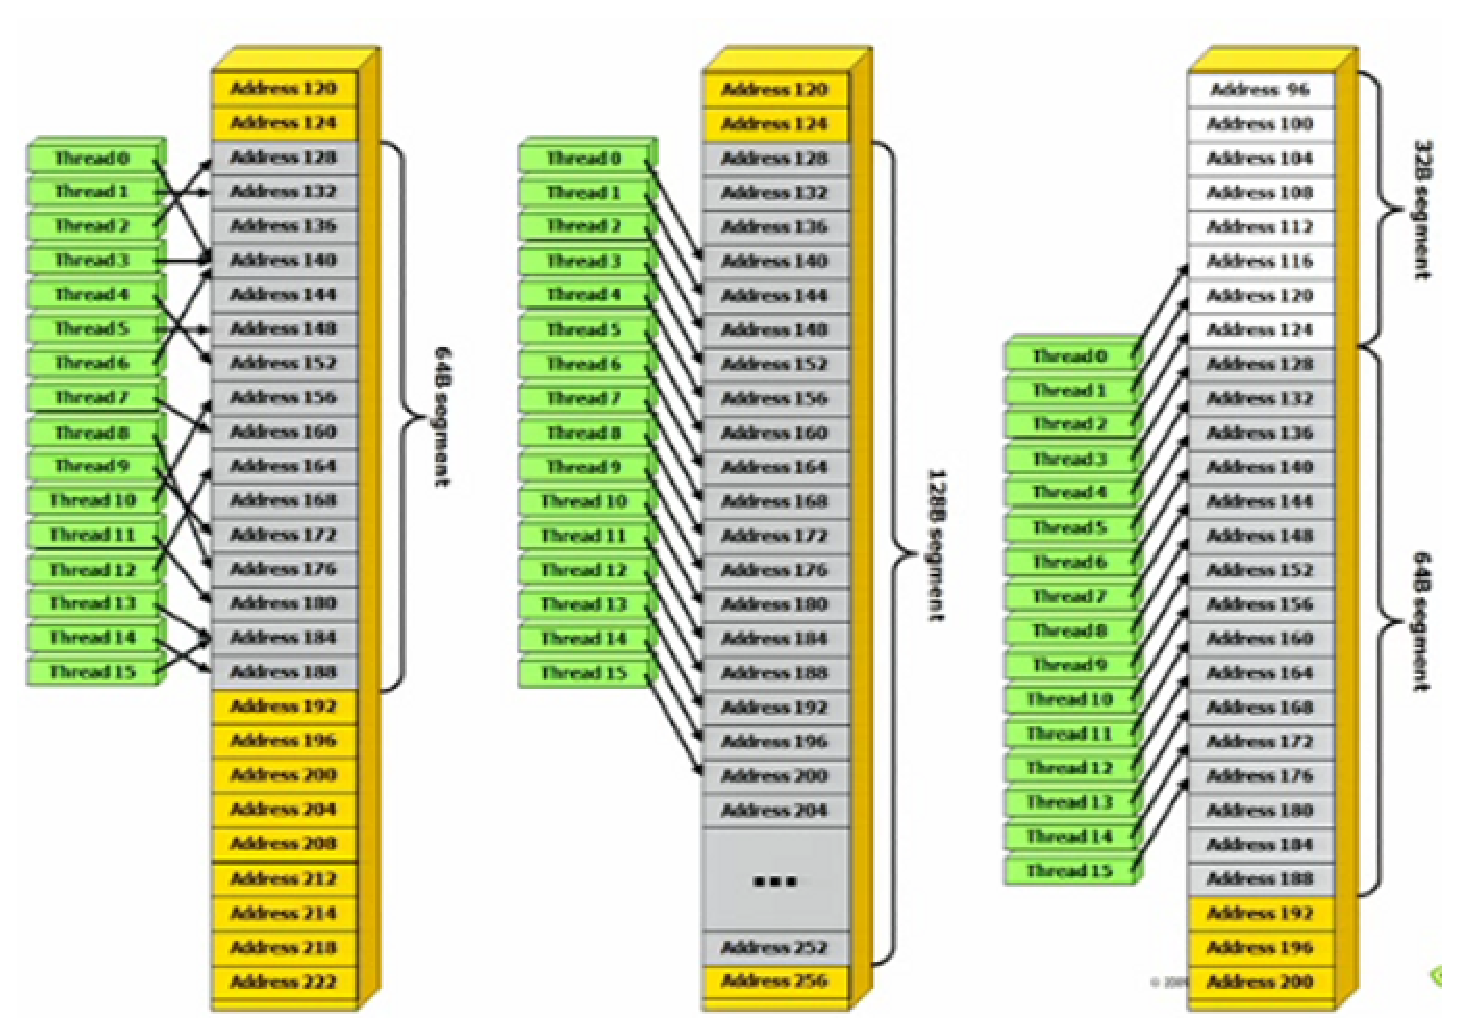
\includegraphics[height=7cm,
    angle=0]{./images/coalesce_memory.eps}}
  \caption{Coalesce memory access}
  \label{fig:coalescing}
\end{figure}

Normally, active threads with lower ID will access data at lower
memory address. The hardware will find the memory segment that
contains the address requested by the lowest ID active thread. If the
data is uncached, i.e. need to read from global memory, the data is
read in group of a given segment size, which is based on the data
element to be accessed
\begin{enumerate}
\item 32-byte segment if data element is 1-byte
\item 64-byte segment if data element is 2-byte
\item 128-byte segment if data element is 4-byte or 8-byte or 16-byte
\end{enumerate}
In any case, try to use {\bf coalescence} whenever possible.  Then,
the hardware find all active threads that have address of memory
request lies in the same segment. Finally, it performs the reduction
of transaction size, if possible.
\textcolor{red}{Typically, an aligned segment is of 32, 64 or 128
  bytes. So, threads with addresses within a segment are served with
  one memory transaction}.

\begin{enumerate}
\item If the segment is 64-byte, and only first-half or second-half of
  the segment is requested, then it reduces to 32-byte segment
\item If the segment is 128-byte, and only first-half or second-half
  of the segment is requested, then it reduces to 64-byte segment. And
  reduction is continued to apply for this 64-byte reduced segment
\end{enumerate}
After carrying the transaction, the hardware mark the serviced threads
as inactive. Then, repeat the process until all threads in the
half-warp are serviced. 


\begin{figure}[hbt]
  \centerline{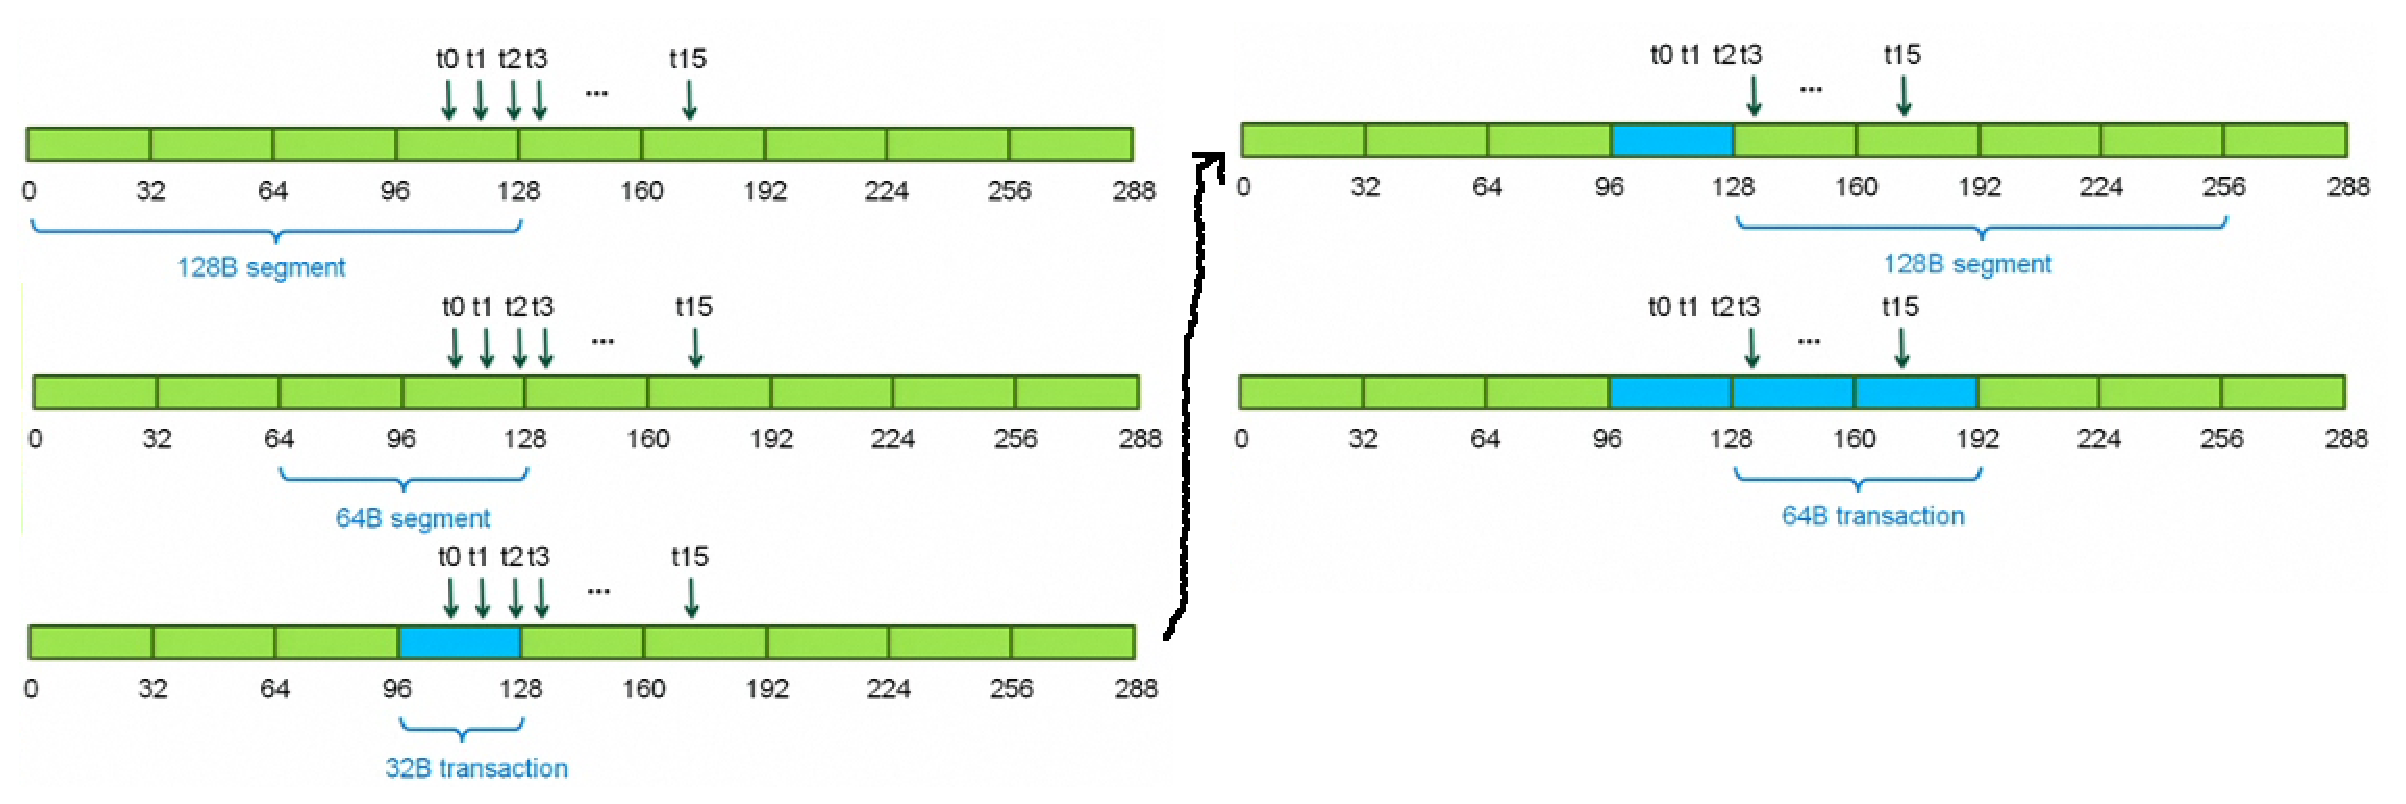
\includegraphics[height=4cm,
    angle=0]{./images/segment_reduction.eps}}
  \caption{Reduction of memory segment}
  \label{fig:segment_reduction}
\end{figure}


{\bf Example}: We have half-warp (threads 0-15) access memory of
4-byte words with address ranging from 116-176. Then, at first the
hardware check the address that thread 0 (the lowest ID) which is 116,
it will use 128-byte segment. In this segment, there are 2 other
threads that access the data within. They are thread 1 and 2. It then
performs the reduction, from 128-byte to second-half 64-byte and next
to second-half 32-byte segment,
Fig.~\ref{fig:segment_reduction}. Similarly, we have the same process
for threads 3 where all other 11 threads (4-15) fit into the
first-half of the 128-byte segment.


Given the hardware process above, there are some other restrictions
\begin{enumerate}
\item On device CC 1.0, 1.1: the $k$-th thread in a half-warp must
  access the $k$-th word in the segment, the starting address for each
  segment is a multiple of 16. The preferred size for each element is
  4-byte.
  \textcolor{red}{If the requirement is not satisfied, then each
    thread has its own 32-byte segment transaction}.

  NOTE: Not all threads need to participate. 

\item On device CC 1.2, 1.3: the $k$-th thread in a half-warp can
  access $j$-th word in the segment ($j$ can be different from $k$) so
  long as no two threads access the same word. % The segment size can be 
  % \begin{itemize}
  % \item 32 bytes for 8-bit words
  % \item 64 bytes for 16-bit words
  % \item 128 bytes for 32-bit words and 64-bit words. 
  % \end{itemize}

  \textcolor{red}{For 64-bit words, each half-warp need to issue 2
    memory access, rather than one}.  % The procedure is given as follow:
  % \begin{enumerate}
  % \item For the lowest numbered active thread, CUDA find the memory
  %   segment that contains the address requested by this thread.
  % \item Given this segment, it will find all active threads which has
  %   memory access to data in this segment. Thus it need to issue only
  %   one memory access, and reduce the transaction size if possible,
  %   then bring back the data for these threads. 
  %   \begin{itemize}
  %   \item If the transaction size is 128 bytes, and only lower or
  %     upper half-warp is used, then it automatically reduce the
  %     transaction size to 64 bytes.
  %   \item If the transaction size is 64 bytes, and only lower or upper
  %     half-warp is used, then it automatically reduce the transaction
  %     size to 32 bytes.
  %   \end{itemize}
  % \item After bring data back to these threads, CUDA mark these
  %   threads in the half-warp as inactive. 
  % \item Repeat until all threads in half-warp are serviced. 
  % \end{enumerate}

\item On device CC 2.0: any thread can access any word, in any order,
  INCLUDING the same word. The reason is that global memory access are
  cached in L1 and L2 (read more in Sect.~\ref{sec:fermi})

\end{enumerate}

\begin{framed}
  As the transaction segment must be aligned, i.e. first address is
  the multiple of the segment size, memory allocated through the
  runtime API, e.g. \verb!cudaMalloc()!, are guaranteed to be aligned
  to at least 256 bytes. 

  It's important that half-warp access a contiguous region or the data
  should be copied to shared memory first, as data location is not
  important in fast shared memory. We will discuss that in
  Sect.~\ref{sec:shared-memory-bank}.

\end{framed}

{\bf Example}: This example show how the offset from perfect alignment
affect to the performance (or aligned case) for 32-bit words. 
\begin{itemize}
\item With 32-byte offset (or 8-word offset), we need to use one
  128-byte segments (load 128-byte but use only 64-byte $\rightarrow$
  50\% efficiency)
\item With 96-byte offset, we need two 32-byte segment  (load 2
  32-byte and use all 64-byte $\rightarrow$ 100\% efficiency)
  \begin{figure}[hbt]
    \centerline{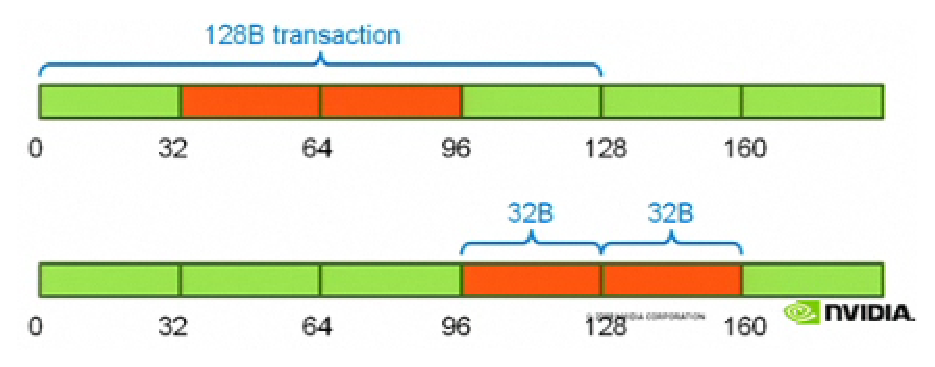
\includegraphics[height=3cm,
      angle=0]{./images/aligned_case1.eps}}
    \caption{Case 1: }
    \label{fig:aligned_offset_1}
  \end{figure}

\item With 16-byte offset (or 4-word offset), we need to use one
  128-byte transaction
\item With 80-byte offset (or 20-word offset), we need to use one
  64-byte segment transaction and one 32-byte segment transaction
  ($\rightarrow$ this is 67\% efficiency)

  \begin{figure}[hbt]
    \centerline{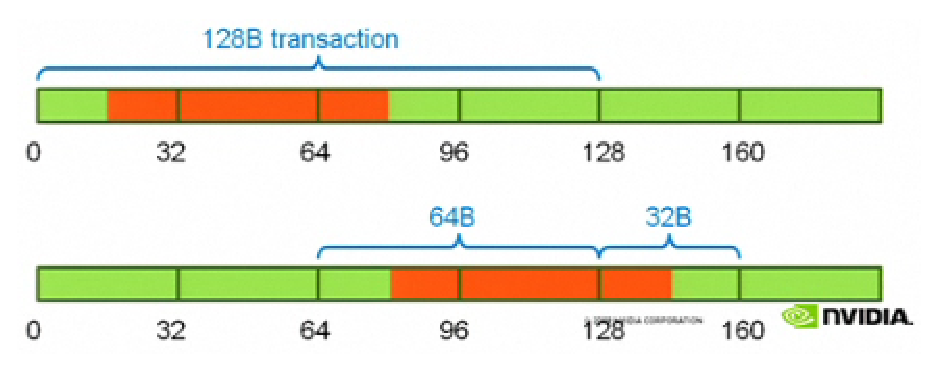
\includegraphics[height=3cm,
      angle=0]{./images/aligned_case2.eps}}
    \caption{Case 2: }
    \label{fig:aligned_offset_2}
  \end{figure}

\end{itemize}

{\bf Example}: This example how the offset from perfect alignment
affect to the performance for 64-bit words.
\begin{itemize}
\item perfect aligned: 80 GB/sec
\item 8-byte offset: 62 GB/sec (78\% efficiency)
\item 16-byte offset: 62 GB/sec (78\% efficiency)
\item 32-byte offset: 68 GB/sec (85\% efficiency)
\item 64-byte offset: 76 GB/sec (95\% efficiency)

  NOTE: Even though both 0-byte offset and 64-byte offset consume all
  read data, 64-byte requires 2 64-byte transactions, and thus a little bit
  slower than using a single 128-byte transaction.
\end{itemize}

The technique to achieve perfect memory alignment in global memory
request is called {\bf coalescing technique}.
\textcolor{red}{In general, memory coalescing techniques are often
  used in conjunction with tiling techniques to reach the ``best''
  performance as possible}.
\begin{enumerate}
\item Use padding if necessary to align the data
\item Threads in a warp should access data within contiguous region
\item Each thread should process several elements as multiple load get
  pipelined
\item Indexing calculation can be reused. 
\item Launch enough threads to cover access latency (NOTE: In GT200,
  global memory access is not cached. But in Fermi, it's cached). 
\end{enumerate}


To hide the arithmetic latency in GT200, we need 6 warps or 192 active
threads in a SM. This is NOT the number of threads per thread
block. For GT200, 50\% occupancy (or 512+ active threads per SM) is
often sufficient. NOTE: Occupancy is the fraction of the maximum
number of threads per SM.

In Fermi, GDDR5 is divided into 6 partitions. It also has additional
improvements over previous generations (e.g. ECC support). 

In Tesla 1
\begin{itemize}
\item DRAM access latency is 400-600 cycles
\item DRAM fire rate latency for uncoalesced access pattern is 300
  cycles
\item DRAM fire rate latency for coalesced access pattern is 40 cycles
\end{itemize}

\subsection{A review}
\label{sec:review}

In DRAMs, data bits are stored in DRAM cells, with very weak
capacitors, each the presence or absence of a tiny amount of
electrical charge distinguishes between 0 and 1. The process of
determining which amount of charge is currently considered 1 (or the
current amount of charge in the capacitor) is a slow process. Thus, to
improve the efficiency, modern DRAMs try to read multiple data
elements, once the status of 0 1 are determined. It means that data
are accessed in burst, i.e. each time a location is accessed, many
consecutive locations, including the requested location, are read
(Sect.~\ref{sec:memory-access}).

To take advantage of bursting access, NVIDIA GPU organize memory
access of threads into favorable patterns.
\textcolor{red}{The most favorable access pattern is threads access
  consecutive global memory locations}.
In this case, the hardware combines, or {\bf coalesces}, all of these
memory accesses into a single access to DRAM.
\begin{itemize}
\item In C, as data are stored in row-major; the more favorable access
  pattern is each thread read a column
  \begin{enumerate}
  \item To access a 4x4 matrix, the elements M[0,1] and M[0,1] are
    placed 4 locations away in the linearly addressed memory. Then, at
    the first load, for all threads to reach consecutive memory
    locations, they must all read the first row. Similarly, in the
    next read, they must all read the second row... Eventually,
    each thread read a column.
  \item If we have to access the data by rows, then we can use shared
    memory to enable memory coalescing. This is discussed in an
    example of matrix multiplication in
    Sect.~\ref{sec:assign-jobs-threads}. On shared memory, it's not
    important whether the access is row basis or column basis as they
    shared memory are designed for intrinsically high-speed, and
    doesn't require coalescing to achieve high data rate. 
  \end{enumerate}
\item In Fortran, as data are stored in column-major; the more
  favorable access pattern is each thread read a row. 
  \begin{enumerate}
  \item If we have to access the data by columns, similar to the
    technique described in CUDA C, we can coordinate the blocks to
    load the data to shared memory first. 
  \end{enumerate}
\end{itemize}
\textcolor{red}{A good experience is that organize your data in structure of arrays
  rather than arrays of structure}. Need an example here. 

What if you access the array element via an indirect indexing
mechanism, e.g. A[indx[i],j], rather than direct indexing,
e.g. A[i,j]? Then, it's better to copy them into a consecutive shared
memory first or consecutive global memory first.
\textcolor{red}{We need an example here}.

A half-warp of 16 threads can read data from global memory
simultaneously in a process known as {\it coalesced memory access},
i.e. consecutive threads in a half-warp read from consecutive memory
addresses. Thus, it is recommended to copy data from global memory to
an array, declared with {\bf shared} attribute to keep the data,
before calling the operation to work on data in this array.
\begin{lstlisting}
attribute(global) subroutine do_this(arr_global, N ...)
 integer, dimension(N) :: arr_global
 integer :: N
 integer, dimension(16), shared :: arr_data

! first, data is read from global to shared memory
 arr_data = arr_global(dim_x:dim_x+16)

! work on arr_data

! save data back to global memory
 arr_global(dim_x:dim_x+16) = arr_data
end subroutine
\end{lstlisting}

{\bf NOTICE}: In certain applications, with operations like
calculating the gradients, or other nearest neighborhood operations,
we need to consider the {\bf border threads}. A border thread is on
the edge of a block, and thus some of its nearest neighbours will be
in the next block and must be accessed through global memory. Under
these circumstances it is appropriate to use
{\bf non-updating border threads}, which act as placeholder
values. This increases the total number of threads to be calculated,
but prevents costly kernel branches and calls to global memory. E.g.:
instead of using 16, we only use 14 indeed, the first lower and upper
threads are served as non-updating border threads.
\begin{lstlisting}
! first, data is read from global to shared memory
 arr_data(1:16) = arr_global(dim_x:dim_x+16)

! work on arr_data

! save data back to global memory
 arr_global(dim_x+1:dim_x+15) = arr_data(2:15)
\end{lstlisting}

To enhance performance, data in global device memory can be cached
into L1 or/and L2 cache memory (Sect.~\ref{sec:shared-memory-cache})
or using Texture memory (Sect.~\ref{sec:texture-memory}). On at cache
misses, does it cost a read from global device memory. So,
\textcolor{red}{try to reduce cache misses, by increase the temporal
  and spatial locality of memory accesses}.
% A cache line is 128 bytes.

Read G.4.2. 


\subsection{Tiling}
\label{sec:tiling}

or each thread calculate not a single element, but a sub-matrix
\begin{lstlisting}
C(x:x+16,y:y+16) = A(x:x+16,y:y+16) * B(x:x+16,y:y+16)
\end{lstlisting}
or you can organize into 2 levels: (1) at level one - the host call a
device subroutine to process a sub-matrix, (2) at level two - the
device subroutine will call kernel subprogram to solve each element in
the sub-matrix, e.g. 
\begin{lstlisting}
C(x:x+16,y:y+16) = A(x:x+16,y:y+16) * B(x:x+16,y:y+16)
\end{lstlisting}
\textcolor{red}{The two former ones are easier, yet the third one is
  sometime more efficient}.
The reason is that both methods need to copy the data from the
off-chip memory to on-chip memory. It's better to copy a bunch of it
at once, and the kernel subprogram can access from the read-only
on-chip memory, rather than leaving each thread copy one by one
directly from the off-chip memory (you will understand this later).

\section{Shared memory and bank conflict}
\label{sec:shared-memory-bank}

Parallel data cache (PDC) or shared memory is on-chip memory, so
accessing to data on shared memory (\verb!__shared__!) is much faster
than data on global memory (i.e. defined as \verb!__local__! or
\verb!__device__!). The purpose of using shared memory is to cache the
data so that threads in a thread block don't have to re-read it from
global memory when the data is reused by (1) more than one threads
and/or (2) more than one time in a thread,
Fig.~\ref{fig:shared_memory}.
\textcolor{red}{Since Fermi, data is automatically cached, so (2) can
  be loosed}.

\begin{figure}[hbt]
  \centerline{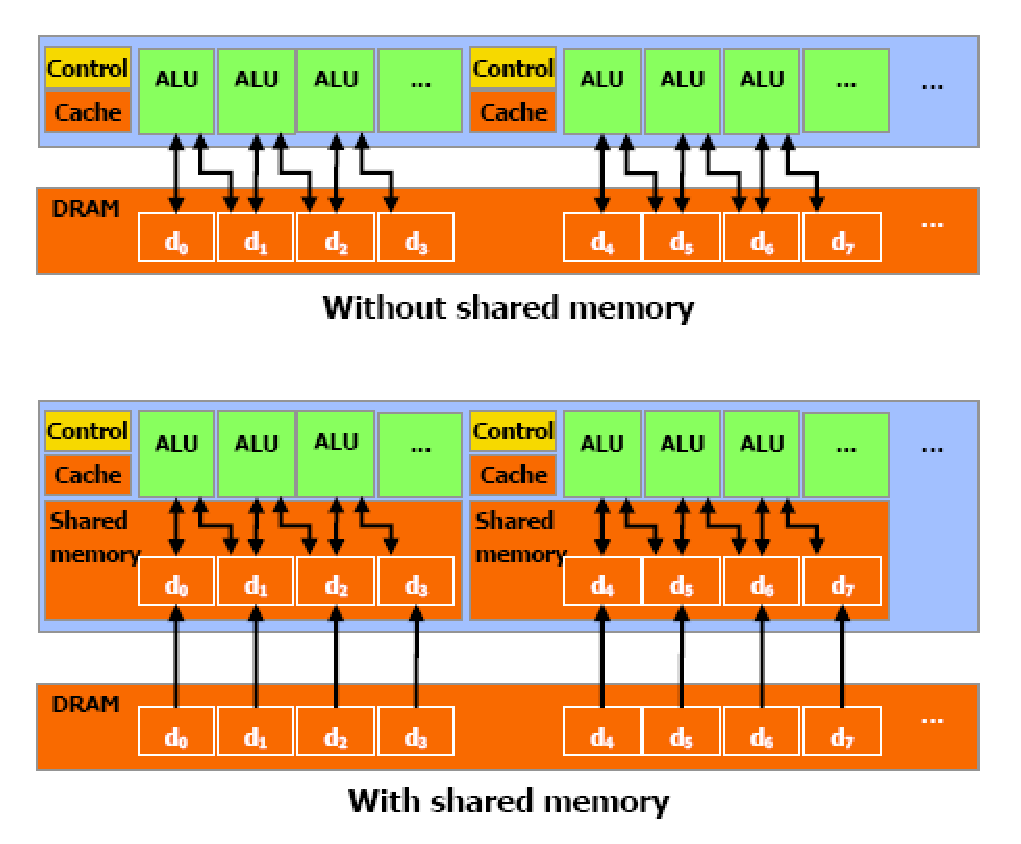
\includegraphics[height=5cm,
    angle=0]{./images/shared_memory.eps}}
  \caption{Demonstration of using shared memory to speed-up memory
    access, and save memory bandwidth}
  \label{fig:shared_memory}
\end{figure}


\subsection{Memory layout organization}
\label{sec:memory-layo-organ}


\begin{framed}
  No matter how many dimension of your data, in CPU, data are
  physically stored in 1D. Any 2D, 3D or higher dimension are mapped
  to 1D by the compiler. This is the same to GPU global device
  memory. However, GPU has special memory space that are designed to
  work best with 2D data. They are known as textures memory. 
  
  Texture memory are read-only, and are limited in size. We will
  discuss that later. 
\end{framed}

There are some technical terms that we need to explain, originating
from graphics. At first, we need to know how the buffer/memory keep
the 1D, 2D or even 3D data in a linear manner. It's easy in 1D
vector. In 2D, the data is stored (in C) row by row, (in Fortran)
column by column. 
\begin{itemize}
\item In C
\begin{verbatim}
A[0][0], A[0,1], A[0,2]..., A[1][0], A[1][1]...
\end{verbatim}
\item In Fortran
\begin{verbatim}
A[1][1], A[2][1], A[3][1]...,A[1][2], A[2][2]...
\end{verbatim}
\end{itemize}
Given that elements in the same columns are adjacent, accessing to
data using column-based 

In 3D, the matrix A[NX][NY][NZ] is stored layer by layer, with a layer
is a 2D array.
\begin{itemize}
\item in C (0-based index): A[x][y][0], A[x][y][1]...A[NX][NY][NZ-1]
  with A[x][y] is stored in row-based as above

\item in Fortran (1-based index): A[1][y][z], A[2][y][z]..., with
  A[y][z] is stored in column-based as above. 
\end{itemize}

\begin{framed}
  Interoperability between C and Fortran: To achieve the same linear
  memory layout, if the data in C is mat[NZ][NY][NX], then the data in
  Fortran should be mat[NX][NY][NZ], with NX varies fastest then to NY
  then to NZ. So, if you want to pass data in Fortran to a C function,
  we need to revert NX and NZ dimension. 
\end{framed}

For example: suppose NX = 2, NY = 3, NZ = 4, to achieve linear memory
with values start from 0 to 23 we need
\begin{multicols}{2}
  \begin{itemize}
  \item in C:
\begin{verbatim}
idx = 0
FOR i = 1, NZ
  FOR j = 1, NY
      FOR k = 1, NZ
         a[i,j,k] = idx
         idx = idx + 1
      END
  END
END
\end{verbatim}
    \columnbreak
  \item in Fortran:
\begin{verbatim}
DO i =1, NX
  DO j = 1, NY
      DO k = 1, NZ
      a[i,j,k] = idx
    idx = idx + 1
  END
    END
    END
\end{verbatim}
  \end{itemize}  
\end{multicols}

\subsection{Memory banks}
\label{sec:memory-banks}

As mentioned in the Sect.~\ref{sec:memory-access}, DRAM memory are
organized into banks. Similarly, shared memory are divided into
equally-sized memory modules, known as {\bf banks}. In CUDA model,
it's optimal when threads in a warp access data at different banks at
a time. This will avoid {\bf bank conflict} that we will discuss in
Sect.~\ref{sec:bank-conflict}.

{\bf Example}: If we have 4 banks, then in Fortran style, it's better
to put each element in a single columns in a separate bank,
Fig.~\ref{fig:bank_sample}. 

\begin{figure}[hbt]
  \centerline{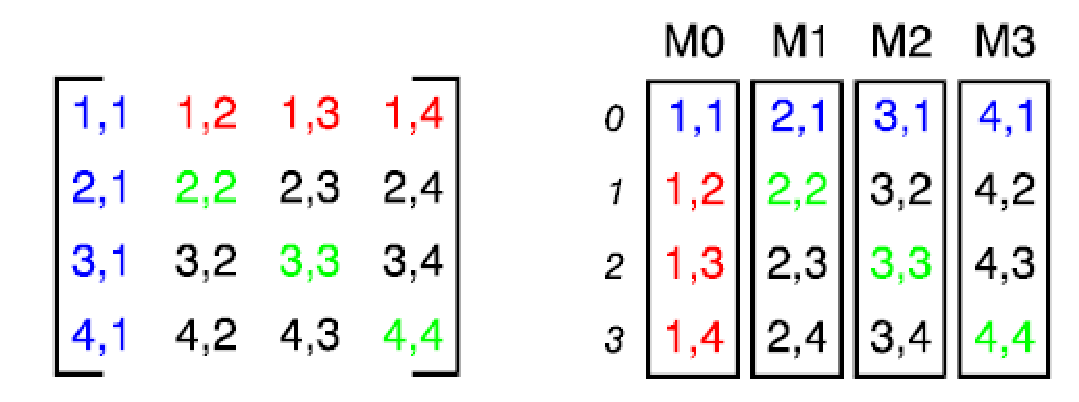
\includegraphics[height=3cm,
    angle=0]{./images/banks_sample.eps}}
  \caption{Sequential elements are stored in consecutive banks}
  \label{fig:bank_sample}
\end{figure}

In practice, due to the limited size of the shared memory, and the
data array may be larger than that, it's often a better choice to load
a portion of the array, known as {\bf tiling}. We will discuss this
technique with different memory access pattern to avoid bank conflict
later.

\begin{enumerate}
\item CC 1.0, 1.1 (e.g. C870): Per SM, shared memory is divided into 16
  banks of single-ported SRAM of equally size, i.e. each bank is
  1KB. 16 banks have total 16KB (i.e. 4096 32-bit words, or each bank
  has 256 32-bit words). The latency, i.e. to read a 32-bit (or
  4-byte) word, is \textcolor{red}{one clock cycle}. Thus, with total
  256KB shared memory on chip, the bandwidth is 675GB/s.

\item CC 1.3 (e.g. C1060): Per SM, shared memory is divided into 16
  banks of equally size, i.e. each bank is 1.5KB. 16 banks have total
  24KB (6144 32-bit word entries or
  \textcolor{red}{each bank holds 384 32-bit
    words}\footnote{32-bit
    is the bank width}).
  The latency, i.e. to read a 32-bit (or 4-byte) word, is
  \textcolor{red}{two clock cycles}. Thus, with 480KB shared memory on
  chip, the bandwidth is ...

\item CC 2.0 (e.g. Fermi): Per SM, shared memory is divided into 32
  banks of equally size, i.e. each bank is 0.5KB or 1.5KB (depending
  on the configuration 16KB or 48 KB (shared/L1 configurable 16/48 or
  48/16)). The latency, i.e. to read a 32-bit (or 4-byte) word,
  \textcolor{red}{two clock cycles}. We will discuss in detail in
  Sect.~\ref{sec:shared-memory-cache}. 
\end{enumerate}

\begin{framed}
  Shared memory is divided into {\bf banks} of equal sizes (see
  below). The number of banks is equal to the number of threads to
  execute in group, i.e. 16 in Tesla 1, 2 and 32 in Fermi. It is
  designed so that one thread access one separate bank at a time, and
  no two threads access the same bank. Otherwise, they need to be
  serialized, i.e. one by one. However, for read-only memory request,
  since CC 1.3, {\bf broadcast} is allowed in the case that $n$
  threads access the same word in one fetch.

  When threads in the group access data to shared memory, if the data
  access pattern violate the architecture design that prohibit the
  simultaneous data access of the threads; then {\bf bank conflict}
  occur. As a result, we need to know which generation of GPU cards to
  know when bank conflict can arise and how to avoid that.

\end{framed}


% The number of memory modules needed to have the same number of data
% bits as the bus. A bank can consist of one or more memory modules.

% We can hide global memory latency and global memory bandwidth
% restrictions so long as there is some local data reuse.

\subsection{Access pattern: stride}
\label{sec:access-patt-stride}

A strided access with stride $k$ means touching
{\it every k-th memory element}.
\begin{enumerate}
\item Stride = 1 is sequential access (0,1,2,3,...)
\item Stride = 2 is (0, 2, 4, 6,...)
\item Stride = 3 is (0, 3, 6, 9,...)
\item Stride = $k$ is (0, k, 2k, 3k, ...)
\end{enumerate}

Strides $>$ 1 is commonly found in multi-dimensional data. For
example:
\begin{enumerate}
\item Row accesses (stride = N) (column-major)
\item Diagonal accesses (stride = N + 1)
\item Image processing (image rows and columns)
\item Scientific computing (e.g. matrix multiplication where we divide
  the matrix into tiles, and assign each tiles to each thread block)
\item Radar/Sonar processing (angle vs. elevation)
\item In many cases, arrays' dimensions are a power of 2 size,
  promoting bank conflict. 
\end{enumerate}

{\bf Conflict reduction techniques}
\begin{enumerate}
\item Software techniques: array size change, i.e. allocate shared
  memory array whose size relatively prime to number of memory
  bank. E.g. in C, before \verb!foo(SIZE, SIZE)!, after
  \verb!foo(SIZE, SIZE+1)!, i.e.  we need to add one to the fastest
  changing dimension. From the example in Fig.~\ref{fig:bank_sample},
  after adding 1 to the fastest changing dimension, row and columns
  access have no conflict. However, with diagonal access, we had 2-way
  conflict, i.e. we need 2 times of accesses.

  \begin{figure}[hbt]
    \centerline{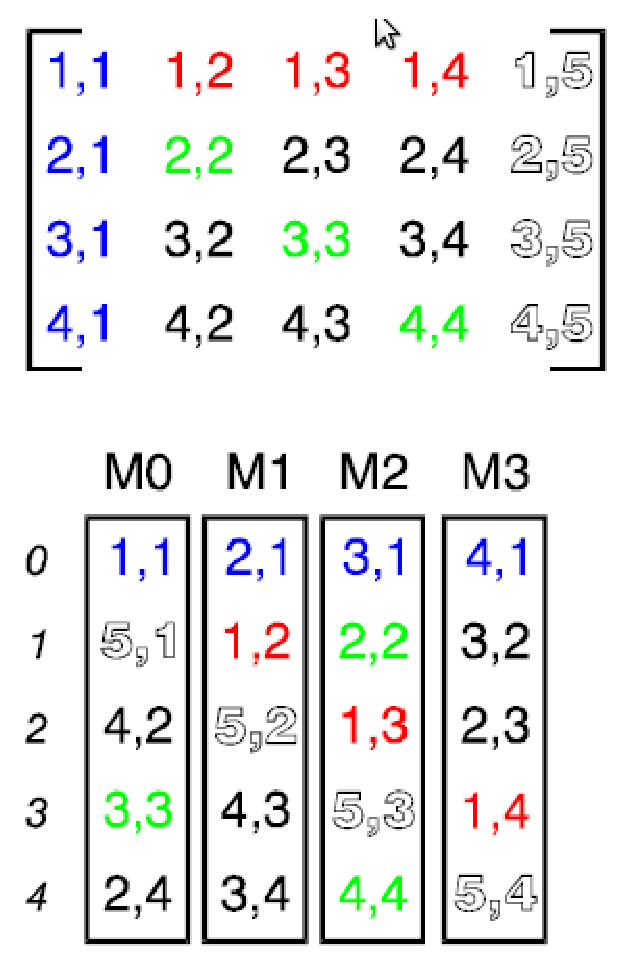
\includegraphics[height=5cm,
      angle=0]{./images/conflict_reduce_1.eps}}
    \caption{Instead of using shared memory of size(4,4), we use
      (4,5). This is row-based }
    \label{fig:conflict_reduce_1}
  \end{figure}

  For example: in CC 1.3
\begin{lstlisting}
// in C
__shared__ float s_a[16][17]
__shared__ float s_a[32][33]
\end{lstlisting}
\begin{lstlisting}
// in Fortran
real, dimension, shared :: s_a(17,16)
real, dimension, shared :: s_a(33,32)
\end{lstlisting}
\item Address modification: skewed addressing,
  e.g. Fig.~\ref{fig:conflict_reduce_2}
\begin{verbatim}
Word address within module = address / #banks
Module # = [ (address/ #banks) + (address * skew) ] MOD #banks
\end{verbatim}

  \begin{figure}[hbt]
    \centerline{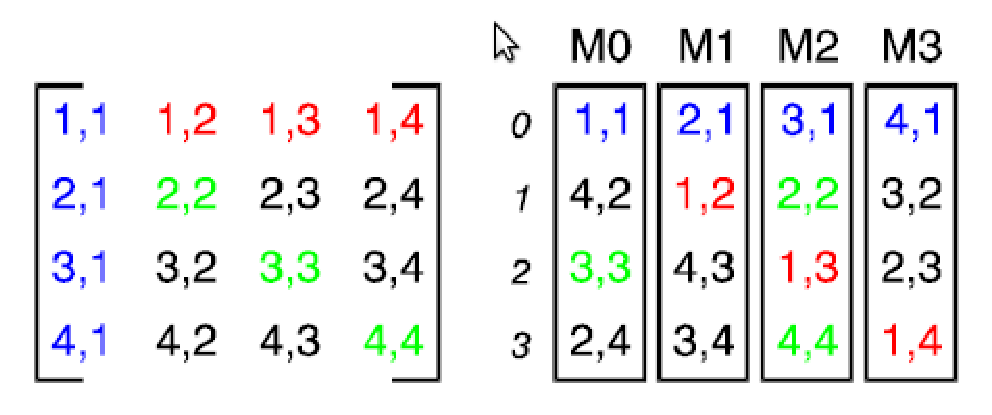
\includegraphics[height=3cm,
      angle=0]{./images/conflict_reduce_2.eps},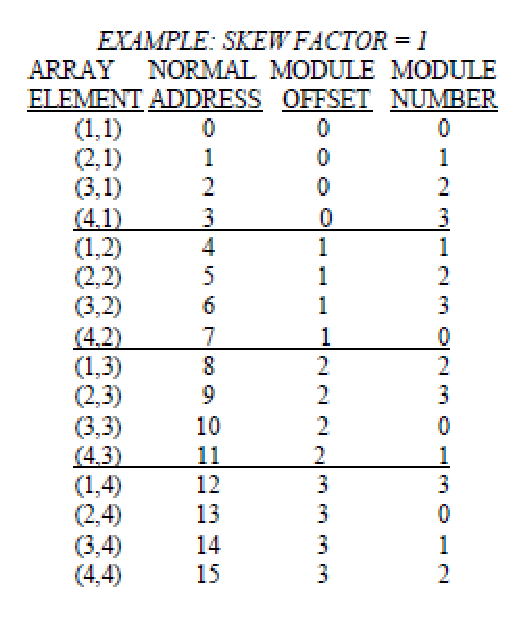
\includegraphics[height=5cm,
      angle=0]{./images/conflict_reduce_2b.eps}}
    \caption{Skew = 1}
    \label{fig:conflict_reduce_2}
  \end{figure}

\item Interleave hardware techniques: prime number interleaving,
  superinterleaving.
  \begin{itemize}
  \item when stride is an even multiple (or divisor) of interleave
    factor\footnote{an interleave factor of 4:1 means for every read
      operations, 4 data elements are skipped before the next
      read}. (1) power of 2 bank size is easy to build (with low order
    bits for bank numbers), (2) power of 2 is a common array size, (3)
    2 divides into all even numbers (and people naturally use even
    numbers) 

  \item prime number interleave reduces possibility of conflicts (good
    tricks for $2^n+1$ or $2^n-1$ banks)
\begin{verbatim}
Bank_# = address MOD num_banks

Bank_address = address MOD words_in_bank
\end{verbatim}
    if \verb!words_in_bank! is a power of 2, then this is simply a shift
    operation. 

  \item Superinterleaving: assume that there are $m$ memory bus cycles
    per module cycle time; then ``normal'' interleaving has $n$ banks
    with $n\cdot m$
  \end{itemize}

  \begin{figure}[hbt]
    \centerline{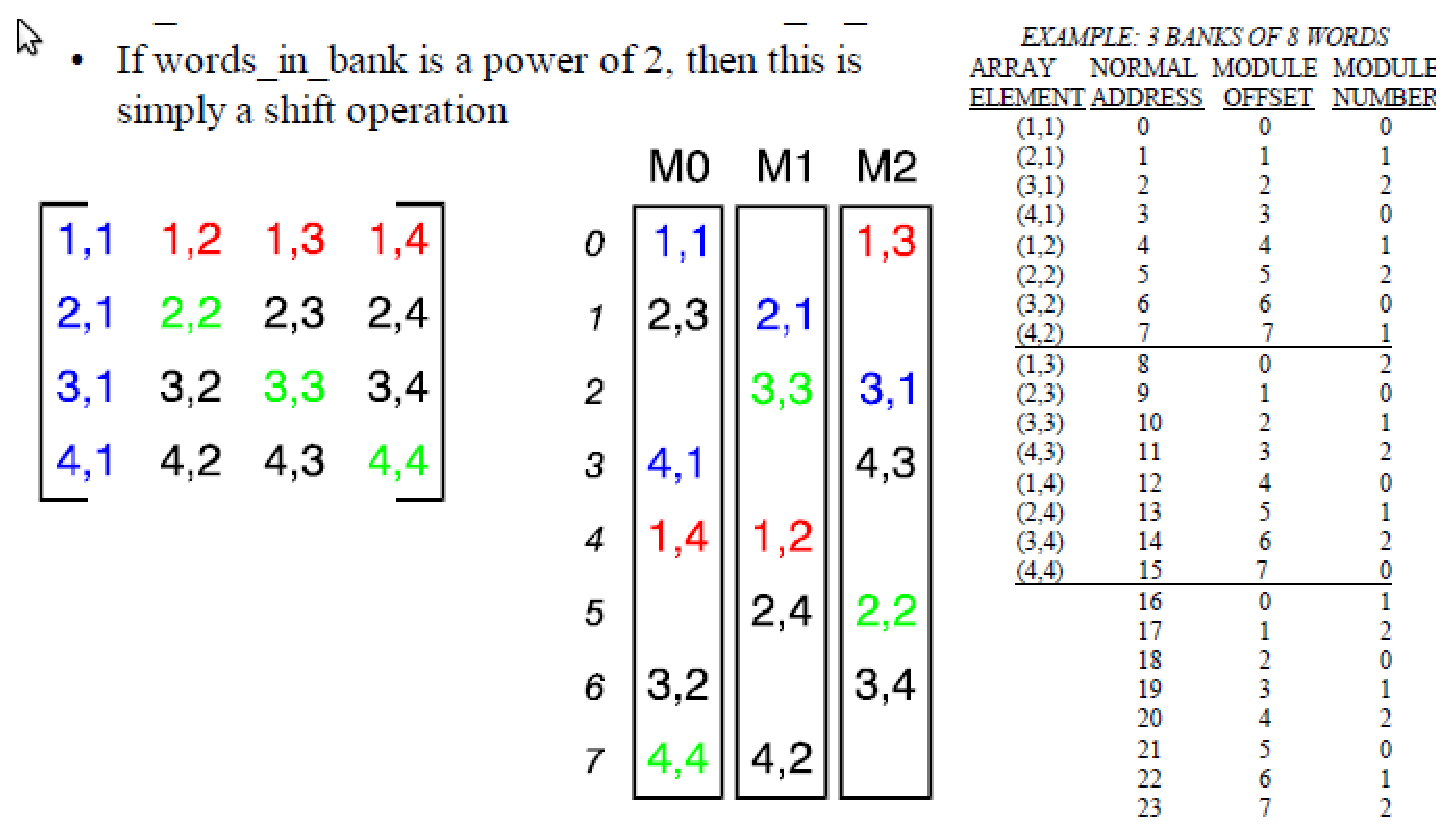
\includegraphics[height=5cm,
      angle=0]{./images/conflict_reduce_3.eps}}
    \caption{3 memory banks, each with 8 words}
    \label{fig:conflict_reduce_3}
  \end{figure}


\end{enumerate}

\subsection{Bank conflict}
\label{sec:bank-conflict}

At first, user need to manually load the data from global to shared
memory. However, how we load the data to shared memory is important as
to avoid {\bf bank conflict}.

If there is no {\bf bank conflict} (to be discussed shortly), access
to shared memory is as effective as to registers. The reason is that
even though accessing to registers is faster (instantly), there is
still the latency ``read-after-write'' in the registers that make
read/write accessing to shared memory is as effective to accessing to
registers.

\begin{framed}
  {\bf Amount of shared memory per SM}
  \begin{enumerate}
  \item C870: each SM (8 SPs) has 16KB shared memory
  \item C1060: each SM (8 SPs) has 24KB shared memory
  \item C2050: each SM (32 SPs) has 64KB configurable memory to
    shared/L1 cache (48/16 or 16/48)
  \end{enumerate}
\end{framed}




\begin{figure}[hbt]
  \centerline{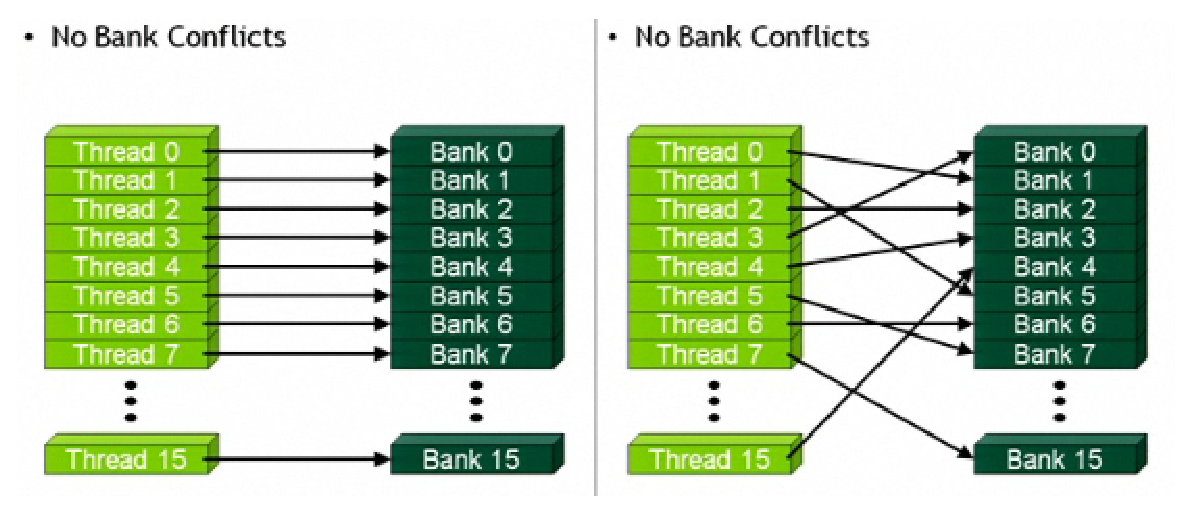
\includegraphics[height=5cm,
    angle=0]{./images/no_bank_conflict.eps}}
  \caption{When each thread use data in a separate bank (in sequential or in
    permutation), there is no bank conflict}
  \label{fig:no_bank_conflict}
\end{figure}

When threads access the same bank, bank conflict occur. Two-way bank
conflict occur when there are 2 and maximum 2 threads access the same
bank which slow the performance 2x. 8-way bank conflict occur when
there are 8 and maximum 8 threads access the same bank,
Fig.~\ref{fig:bank_conflict}.

\begin{figure}[hbt]
  \centerline{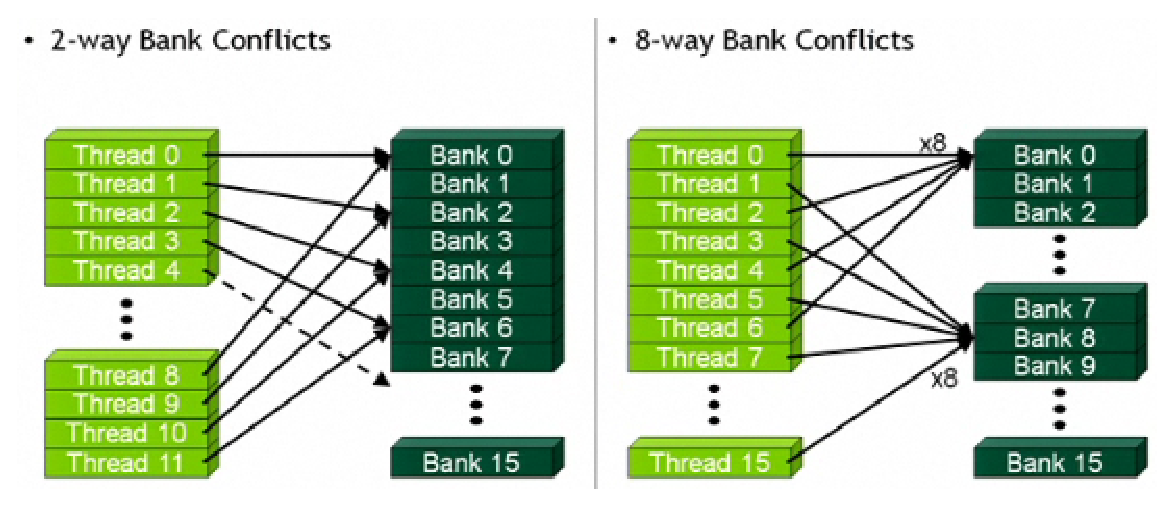
\includegraphics[height=5cm,
    angle=0]{./images/bank_conflict.eps}}
  \caption{When two or more threads use data in the same bank, bank
    conflict occur}
  \label{fig:bank_conflict}
\end{figure}

\textcolor{red}{Beside data coalescing in global memory access,
  knowing how to avoid bank conflict when using shared memory is an
  important technique that we need to master, read G3.x and G4.x in
  the CUDA Programming Guide}. Here are some tricks
\begin{itemize}
\item shared memory read (SMEM read) to the same value, i.e. use the
  same index array. $\rightarrow $ broadcast and no conflict.
\item shared memory write (SMEM write) $\rightarrow$ replace the
  array index with \verb!threadIdx.x!, which can also be done to SMEM
  read. 
\end{itemize}

To assess the efficiency of using shared memory, we use {\bf memory
  access redundancy} which is the ratio of the number of elements
accessed to the number of elements processed. Here, the lower bound is
1, and the smaller the value is the better the performance. 
If possible, we also use {\bf read redundancy}, which does not include
writes in the access count; or {\bf write redundancy} which does not
include write in the access count. 


Sequential threads within the same warp are accessing locations that
are exactly \verb!BLOCK_SIZE! apart, which will cause bank conflicts
if \verb!BLOCK_SIZE! is a multiple of 16. So, in Tesla 1 + 2, we need
to do this differently
\begin{itemize}
\item 1D:

\item 2D:
\begin{lstlisting}
  __shared__ float a[BLOCK_SIZE][BLOCK_SIZE+1];
  __shared__ float b[BLOCK_SIZE][BLOCK_SIZE+1];
\end{lstlisting}
  and in Fortran
\begin{lstlisting}
real, shared :: a[BLOCK_SIZE+1][BLOCK_SIZE];
real, shared ::  b[BLOCK_SIZE+1][BLOCK_SIZE];
\end{lstlisting}
  This causes sequential threads to access locations that are
  \verb!BLOCK_SIZE! + 1 apart, and if \verb!BLOCK_SIZE! is a multiple of
  16, then all the threads in a half warp will access different banks.

  The tiling doesn't have to be square, e.g. 32x4, 12x16, yet it is
  often used as square. 

  Now, let's see how many resident thread block per SM based on shared
  memory usage. In Tesla 2, shared memory has 16kB per SM.
  \begin{itemize}
  \item if tile size is 32x32, then as given in the example above, a
    single thread block need two shared memory blocks As[32][32] and
    Bs[32][32] (each element is 4-byte) which takes 8kB, so only one
    thread block can be put into SM.  ( not 2 thread blocks per SM since
    parameters of kernel function also occupy shared memory and other
    special variables are stored in shared memory as well,
    e.g. \verb!blockIdx!, \verb!blocDim!, \verb!gridDim!, so you can
    use <16KB shared memory)

  \end{itemize}
\item 3D:
\end{itemize}

\begin{lstlisting}
  a[threadIdx.y][threadIdx.x] = A.elements[posA.y * A.width + posA.x];
  b[threadIdx.y][threadIdx.x] = B.elements[posB.y * B.width + posB.x];

  __syncthreads();

// iterate over a row in the copied sub matrix a (a column in sub matrix b)
  for (int e = 0; e < BLOCK_SIZE; ++e)
    cValue += a[threadIdx.y][e] * b[e][threadIdx.x];
\end{lstlisting}
In 2D, the tiling size \verb!BLOCK_SIZE! can be tested with 1, 2, 4,
8, 16 and 32. If each thread in the block process one tiling element,
then \verb!BLOCK_SIZE!*\verb!BLOCK_SIZE! should not excess max threads
per SM (or 512 with Tesla 2). So, 32 is not a legal value. 



\subsection{Tesla 1, Tesla 2}
\label{sec:tesla-1-tesla}

\begin{framed}
  NOTE: 1 word = 32-bit, e.g. a float
\end{framed}

Shared memory is divided into 16 memory banks. Within each cycle, it
is possible to access each of the 16 banks via 16 internal buses of 32
bits (or 512 bits altogether). As an access instruction to this memory
is processed by warps or by groups of 32 threads, these are in fact 32
memory accesses in two cycles that have to be processed. The first 16
threads will be processed during the first cycle and the next 16 in
the second cycle. Two simultaneous accesses to the same memory bank
can't be processed in the same cycle. Each of the first 16 (or last)
threads will have to access a different bank or else several cycles
will be required. It's interesting to note that all threads can access
the same bank. This shows the complexity of the utilization of this
shared memory if the objective is to maximize performances. This isn't
cache memory like CPU use and it is closer, for example, to the local
memory of the SPEs of the Cell.


(Tesla 1,2) Data stored in shared memory is ``stripped'' across the 16
banks, i.e. bank 0 holds words (0, 16, 32, 48, 64...), bank 1 holds
words (1, 17, 33, 49, 65...), bank 2 holds words (2, 18, 34, 50,
56...).
\textcolor{red}{It's important to know that words here are 32-bit. If
  we want to use data in double-precision, we need special handling,
  to be discussed later}.

In CC 1.0/1.1/1.2/1.3, threads are launched in groups of size
half-warp. Ideally, to avoid bank conflict in a half-warp, two threads
in a half-warp must NOT access data in the same bank, i.e. if thread 0
access data 0, then the other 15 threads cannot access data 16 or 32
... Here, we EMPHASIZE data to be 32-bit, and pitch of 16. If the data
to be 64-bit, the pitch is 8.

\begin{itemize}
\item CC1.0, 1.1 (e.g. C870): thread $k$-th (of the same half-warp)
  must access data on the $k$-th bank; otherwise; bank conflict occur
\item CC1.2, 1.3 (e.g. C1060): two threads (of the same half-warp) can
  access data on any bank; as long as no two threads access data on
  the same bank.
\end{itemize}

\textcolor{red}{A conventional method to avoid bank conflict is to use
  {\bf padding}. Another, yet simpler way is to convert from row-major
  access to column-major access (for C language)}. 

{\bf Example 1}: Fig.~\ref{fig:bank_no_conflict}, each 3-word structure
is written across 3 sequential banks. So, each thread per half-warp
can read, say the first structure element,  from one of 16 banks per
two clock cycles without conflicts, i.e. there is no ``.x'' structure
element from two structures residing on the same bank.

\begin{figure}[hbt]
  \centerline{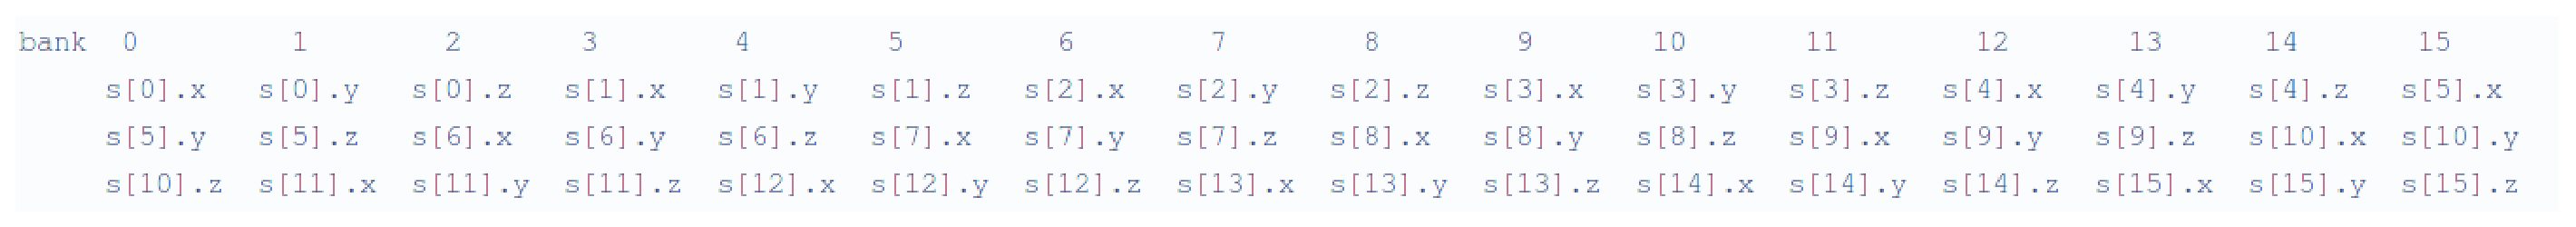
\includegraphics[height=1cm,
    angle=0]{./images/no_bank_conflict_2.eps}}
  \caption{Example of no bank conflict (``s'' denotes shared memory)}
  \label{fig:bank_no_conflict}
\end{figure}

{\bf Example 2}: Each thread access a 32-bit word from an array index by
thredID ``tid'' and with some {\bf stride} ``s''.
\begin{lstlisting}
__shared__ float shared[32];
float data = shared[BaseIndex + s * tid];
\end{lstlisting}
The threads ``tid'' and ``tid+n''' will access the same bank
(i.e. bank conflict), whenever
\begin{verbatim}
BaseIndex + s*tid mod m = BasedIndex + s*(tid+n) mod m
\end{verbatim}
with $m$ is the number of banks. Or ``s*n'' is a multiple of the $m$,
i.e. $n$ is a multiple of $m/d$ with $d$ is the greatest common
divisor of $m$ and $s$. As $m$ is a power of two, e.g. 16 or 32, and
$n=15$ in Tesla 1, Tesla 2.
\begin{itemize}
\item if $s$ is odd, then $d=1$. Then no bank conflict when $n$
  smaller than $m$
\item If $s$ is even, e.g. $s=2$, then $d=2$. Then no bank conflict
  when $n$ smaller than $m/2$, which is impossible. So, bank conflict
  occur.
\end{itemize}

{\bf What if the data element is not 32-bit, but smaller or larger
  than that?}

{\bf Example 3}: A data element is 8-bit (char)
\begin{lstlisting}
__shared__ char shared[32];
char data = shared[BaseIndex + s * tid];
\end{lstlisting}
\begin{itemize}
\item If $s=1$, then shared[0], shared[1], shared[2], shared[3] are
  ``within'' 32-bit word of the same bank. 
\item If $s=4$, then the bank conflict can be avoided
\end{itemize}

{\bf Example 4}: A data element is a structure
\begin{lstlisting}
__shared__ struct type shared[32];
struct type data = shared[BaseIndex + s * tid];
\end{lstlisting}
There are many situation can occur, depending on the types of the
struct element
\begin{itemize}
\item IF 
\begin{lstlisting}
struct type{
  float x, y, z;
}
\end{lstlisting}
  then each member fit to a single 32-bit word. So the whole struct is
  accessed with a {\bf stride} of 3
  32-bit-words. \textcolor{red}{There is no bank conflict}.

\item IF 
\begin{lstlisting}
struct type{
  float x, y;
}
\end{lstlisting}
  then each member fit to a single 32-bit word. So the whole struct is
  accessed with a {\bf stride} of 2 32-bit-words.
  \textcolor{red}{There is bank conflict}.

\item IF 
\begin{lstlisting}
struct type{
  float x;
  char c;
}
\end{lstlisting}
  then the first member fit to a single 32-bit word, while the second
  member take only 8-bit. The {\bf stride} is 5 8-bit-words.
  \textcolor{red}{There is bank conflict}.
\end{itemize}

{\bf Example 5}: There is 2-way bank
conflict\footnote{$n$-way bank conflict means it needs $n$ separate
  memory request}
involving shared memory with double precision data, which can be
avoided if we break the variable into hi and lo parts (Programming
Guide) and then access it, but it's a pain.
\begin{lstlisting}
__shared__ double shared[32];
double data = shared[BaseIndex + s * tid];
\end{lstlisting}
\begin{enumerate}
\item One way to avoid bank conflict is to split the {\bf double}
  operand like
\begin{lstlisting}
__shared__ int shared_lo[32];
__shared__ int shared_hi[32];
double dataIn;

shared_lo[BaseIndex + tid] = __double2loint(dataIn);
shared_hi[BaseIndex + tid] = __double2hiint(dataIn);

double dataOut = __hiloint2double(shared_hi[BaseIndex + tid],
shared_lo[BaseIndex + tid]);
\end{lstlisting}
  \textcolor{red}{However, it might not improve performance, and will
    perform worse on future architecture (Fermi)}.

\end{enumerate}


\begin{framed}
  To avoid bank conflict in ``read-only'' operations, shared memory
  has a {\bf broadcast} feature that a single 32-bit word can be read
  and broadcast to several threads with only one memory request. A
  common example is when all threads read from an address ``within''
  the same 32-bit word. Fermi has a new feature called {\bf
    multicasting}. 
\end{framed}



\subsection{Prefetching data}
\label{sec:prefetching-data}

Accessing to global memory is slow, and tiling techniques is a
solution for using shared memory to address this problem.

The purpose of using multiple active warps in CUDA is that while some
warps waiting for their memory access results, some other active warps
can use the resources to process other instructions. This is a very
powerful mechanism, yet may not be sufficient when all threads are
waiting for their access results. This may be the case when all
threads have a very small number of independent instructions between
memory access instructions and the consumer of the data accessed. 

A solution to the above problem is to prefetch the next data elements
while consuming the current data elements. 
\begin{verbatim}
//Without prefetching
Loop {
  Load current tile to shared
  memory
  __syncthreads();

  compute current tile
  __syncthreads();
}
\end{verbatim}


\begin{verbatim}
Load first tile from global memory into registers

Loop {
  Deposit tile from registers to shared memory

  __syncthreads();
  Load next tile from global memory into shared registers

  Compute current tiles

  __syncthreads();
}
\end{verbatim}

\section{Access pattern: 2D or 3D stencil computation}
\label{sec:2d-or-3d}

You are recommended to read Sect.~\ref{sec:memory-layo-organ} first.
A stencil code is a computer code that update array elements based on
some fixed patterns, which is called stencils. Stencils-based
computations is widely used in solving partial differential equation
(PDE) (e.g. finite element methods), image processing ...

PDE solvers constitutes a large fraction of scientific applications
like heat diffusions, electromagnetics, fluid dynamics, etc. In
stencil computation, each grid point in a multidimensioinal grid is
updated with weighted contributions from a subset of its neighbors in
both time and space. The solvers range from simple Jacobi iterations
to complex multigrid and adaptive mesh refinement methods. 

\begin{framed}
  An order-$k$ stencil refers to a stencil that requires $k$ input
  elements in each dimension, not counting the element at the
  intersection.

  Depending on the number of the dimensions in used, we have different
  value from the $m$-point stencil. Normally, $m=2d\times k + 1$ with
  $d$ is the number of dimensions. 
\end{framed}

In Fig.~\ref{fig:5-point_stencil}, it shows an 1D order-2 stencil, and
2D order-2 stencil. Here, at every iteration, the center element
update itself by computing using the value from 4 of its neighbors. 

\begin{itemize}
\item 1D order-$k$ stencil needs ($2k$+1) points
\item 2D order-$k$ stencil needs ($4k$+1) points
\item 3D order-$k$ stencil needs ($6k$+1) points
\end{itemize}
\begin{figure}[hbt]
  \centerline{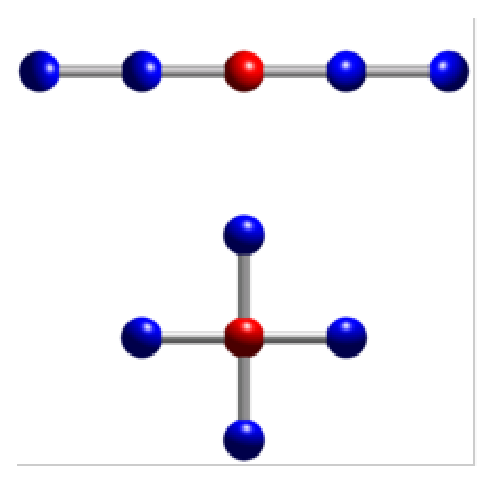
\includegraphics[height=5cm,
    angle=0]{./images/5-point_stencil.eps}}
  \caption{5-point stencil in 1D and 2D}
  \label{fig:5-point_stencil}
\end{figure}

Challenges:
\begin{enumerate}
\item whole data structures are typically much larger than the
  capacity of the available data caches.
\item data re-use is limited to the number of points in a stencil,
  which is typically small. 
\end{enumerate}
So, mostly the bottle-neck is the memory bound, not the computational
bound since data from main memory cannot be transferred fast enough to
avoid stalling the computational units (cores). 


{\bf Example}: In many cases, we have a grid of 3D arrays of
doubles. In every iteration, the center elements update itself by
computing using 6 of its neighbors (two in each dimension), and
itself. The widely used method is finite difference computation,
e.g. the 3D heat equation
\begin{equation}
  \label{eq:7}
  \begin{split}
    B[i,j,k] = C_0A[i,j,k] + C_1(A[i-1,j,k+A[i,j-1,k]+A[i,j,k-1] \\
    + A[i+1,j,k]+A[i,j+1,k]+A[i,j,k+1])
  \end{split}
\end{equation}
This is 7-point stencil. We need read and write performed in two
distinct arrays. Here, we need 8 floating-point operations, yet upto
24bytes (for write-allocate architecture) or 16bytes
(otherwise). NOTE: that problems with the flop:byte ratio less than
0.33 or 0.5 flops per byte are likely to be memory bound. 

In C, multidimensional arrays are most generally handled simply by handling the strides "by hand".  That is, to access 3D array A at (i,j,k), you can simply do

\begin{verbatim}
A[i*istride + j*jstride + k*kstride] 
\end{verbatim}

Often, kstride is implicitly 1.  In C++, this can be hidden with an
inline member function which overrides the [] or () operator, so you
can just use A(i,j,k) or A[i,j,k] according to your preference.  If
I'm not mistaken, this inlining is very simple and does not require
any of Fermi's new hardware features, but just requires support from
the nvcc compiler.  I am not certain whether this works at present or
not.

The older way of doing this in C is to define a preprocessor macro
such as
\begin{verbatim}
#define A3(i,j,k) A[(i)*istride +((j)*jstride + (k)*kstride] 
\end{verbatim}
which assumes you've define istride, jstride, and kstride before using
the macro.  Then you can use A3(i,j,k) as you would expect.  I'm not
sure if this is the kind of support you were looking for.

References:
\begin{itemize}
\item
  \url{http://developer.download.nvidia.com/CUDA/CUDA_Zone/papers/gpu_3dfd_rev.pdf} 
\item \url{http://www.cs.berkeley.edu/~volkov/volkov10-parcfd.pdf}
\item \url{http://www-vis.lbl.gov/Publications/2010/LBNL-3425E.pdf}
\end{itemize}

\section{Shared-memory and Cache - review}
\label{sec:cache-review}

Cache is fast and small memory which is used to hold copies of data on the main
memory to speed up the data fetch and store, eventually to enhance the
performance.

\subsection{Cache line}

Data is moved between the cache and memory not in single byte, but in the unit
of so-called cache lines. A {\bf cache line} describes the size of a chunk of
contiguous data that must be copied into or out of a cache in one operation.
\textcolor{red}{In other words, a {\bf cache line} refers to the minimum amount
of data read in for a single memory operation}. The size of cache and cache line
vary with processor used. Each cache line has the {\bf tag} referring to the
index (or the address) of the data in the main memory. The purpose of using
cache line is for data reuse, so to minimize number of I/O if possible by
reading not a single data but a chunk of them.


\begin{figure}[hbt]
  \centerline{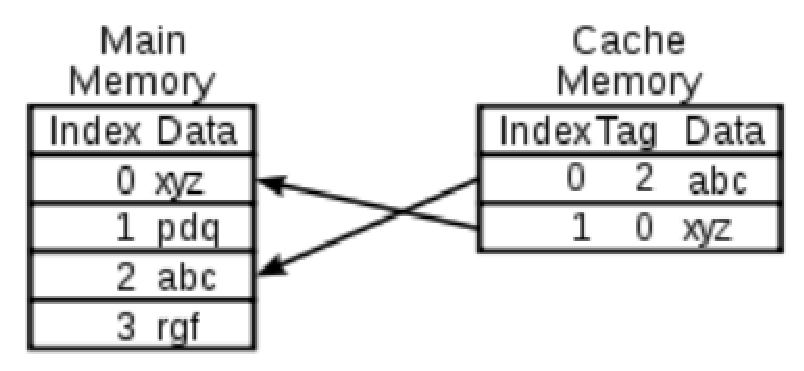
\includegraphics[height=3cm,
    angle=0]{./images/cache.eps}}
  \caption{Cache: index indicate the cache line, tag indicate the
    index of the original data in the main memory}
  \label{fig:cache}
\end{figure}

Typically, cache-line in L1 cache is bigger and cache-line in L2 cache is
smaller. Depending how often cache miss occurs, you should choose between using
bigger cache-line or smaller cache-line. In GPU, knowing that L1 share/cache can be configured to
use as cache. If we use L1 as cache, then L2 cache-line should follow that of
L1. So, it's important to know the difference to choose between using only L2 as
cache or L1/L2 as cache. The exact value for cache-line of L1 and L2 cache can
be referenced in Sect.\ref{sec:shared-memory-cache}.

\subsection{Cache hits/miss}

When the system want to write/fetch data to/from a memory location in
the main memory, it first check if the address is contained in the tag
of any cache line now mapping in the cache. If it finds, then a
{\bf cache hit} occur, which is a good news. Otherwise, we call it a
{\bf cache miss} and the cache line containing the address of the
requested data is moved to the cache. Clearly, this cache line
contains other data that was not specifically requested. If the
granularity of the cache line is 128-byte, then even though you read a
single data element of 8 bytes, and a cache miss occur, another unused
120 bytes are also read to the cache. So, it's important to maximize
the reuse of data in the cache line 

\begin{itemize}
\item For reach cache miss: it take long as the data need to be read
  from the main memory to the cache first.
\item For write cache miss: we may avoid such penalty as the data from
  the main memory is unused. The delay is mainly the creation of a new
  cache entry. 
\end{itemize}

\begin{framed}
  Data in a cache line is subject to reuse if, while the line is
  encached, any of the data elements contained in the line besides the
  originally requested element are referenced by the program, or if the
  originally requested element is referenced more than once.
\end{framed}


\subsection{Misaliged/Aligned data}

Aligning data addresses when allocating memory to match cache line boundaries
allows for efficient data reuse in loops. If data is misaligned, then you may
need more I/O request to the high-latency memory than it should be and thus
decrease the performance.  In CPU, Fortran align data on 32-byte boundary (for
data object larger than 32 bytes), and 64-byte boundary (for data object larger
than 64 bytes). Data aligned on 64-byte boundary is created using
\verb!ALLOCATE()! (Fortran) or \verb!malloc()! or \verb!memory_class_alloc()!
(in C). When using multi-dimensional array, it's thus important that the
starting address of the second-dimension should be at a location of multiple of
32- or 64-, depending on the boundary constraint.

\textcolor{red}{To prevent data following the first array from becoming
  misaligned, scalar variables should be listed after arrays and ordered
  from longest data type to shortest. For example, REAL*8 scalars should
  precede REAL*4 scalars}. Example: In C, array [3,20] of \verb!float! type
\begin{verbatim}
a[0,0], ... a[0,19],a[1,0], .. a[1,19],a[2,0],.. a[2,19]
\end{verbatim}
First dimension is of 20*sizeof(float)=80-byte. Given the 32-byte boundary, we
need to patch 16-byte so that each dimension is 80+16=96 divided by 32. So, we
do
\begin{verbatim}
malloc(a, 96*20, sizeof(float))
\end{verbatim}
If the data is not alliged, then cache miss occurs frequently. The situation is
known as {\bf cache thrashing}.

{\bf Cache thrashing} is the situation where main memory is accessed
in a pattern that leads to different frequently used main memory
locations competing for the same cache lines, resulting in excessive
cache misses. This is most problematic for caches that have low
associativity. 

{\bf Example}: cache thrashing happen in 2MB-cache. Here, we use
COMMON block so that the three arrays are allocated in contiguous
memory in the order shown. The number of elements 131072 means each
array occupy 1MB. In this case,, ORIG and DISP have identical cache
addresses. With cache line 32-byte, once we load the 1st value
(8-byte) in cache, the 2-4 values are loaded as well. So that we only
need a single memory access for 4 computation.  However, as elements
of the same index in ORIG and DISP share the same a cache address;
this cannot happen as they thrash each other. 
\begin{lstlisting}
REAL*8 ORIG(131072), NEW(131072), DISP(131072)
COMMON /BLK1/ ORIG, NEW, DISP
.
.
.
DO I = 1, N
  NEW(I) = ORIG(I) + DISP(I)
ENDDO
\end{lstlisting}
To avoid this, we pad some data in between. With 32-byte boundary
cache line, we need to pad 32-byte
\begin{lstlisting}
REAL*8 ORIG(131072), NEW(131072), P(4),DISP(131072)
COMMON /BLK1/ ORIG, NEW, P, DISP
! or

REAL*8 ORIG(131072), NEW(131076), DISP(131072)
COMMON /BLK1/ ORIG, NEW, DISP

! or even higher 
REAL*8 ORIG(131072), NEW(131080), DISP(131072)
COMMON /BLK1/ ORIG, NEW, DISP
\end{lstlisting}


Principles of good cache uses: maximize locality
\begin{itemize}
\item (spatial locality) try to make use of every word in every cache
  line it touches
\item (temporal locality) use a cache line intensively and not return
  to it later
\end{itemize}

{\bf Example}: A matrix multiplication using column-major arrays,
Fig.~\ref{fig:cache_line}. Each cache line whole the columns from the
arrays. 
element. 
\begin{itemize}
\item Suppose the matrices are small enough, that we have enough
  cache to hold the whole matrices A and B, then there is no problem. 
  In addition, the cache lines are reused. 

\item What if we don't have enough cache to hold the whole matrices,
  i.e. there can't be no re-use in cache lines. Assume the cache line
  can hold a single whole column. As you can see, B is traversed in a
  single column, i.e. all elements in the cache line are traversed
  (i.e. good spatial locality). However, at each cache line that whole
  A's column, it use only a single value from the cache line. It means
  we don't have good temporal locality. 
\end{itemize}
One common strategy in using shared memory is that we hold a tiling of
size $8\times 8$ or $16\times 16$. In terms of cache, the size of a
cache line is limited.  The size for each cache line varies in
different design, e.g. from 8 to 512 bytes.


\begin{figure}[hbt]
  \centerline{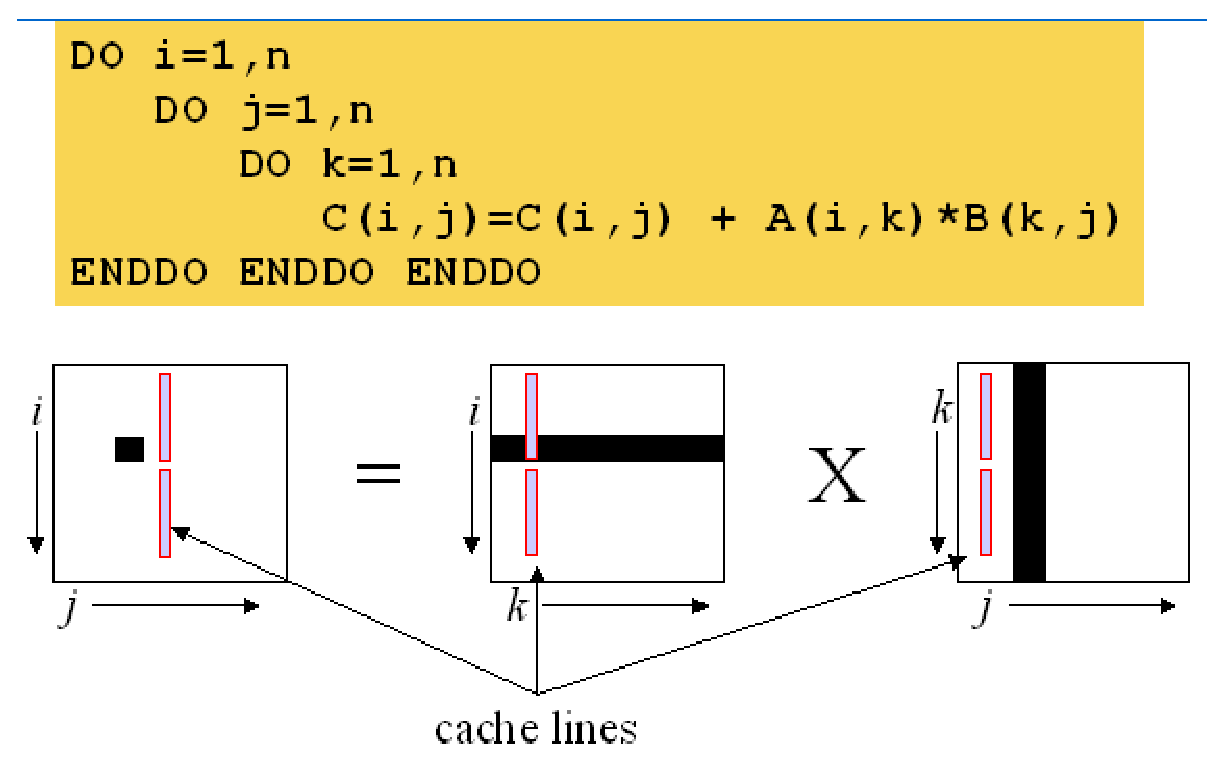
\includegraphics[height=5cm,
    angle=0]{./images/cache_line_ex1.eps}}
  \caption{Each cache line keep a column of each matrix}
  \label{fig:cache_line}
\end{figure}

\subsection{Fermi architecture}
\label{sec:shared-memory-cache}

In Fermi L1 or L2 cache, a cache line is 128-byte line and map to
128-byte aligned segment in global memory. So, with 32 threads per
warp, it's best if each thread in the warp access 4-byte data element
and the data are consecutive. In that case, only a single memory
request is needed for the whole 32 threads. However, if the thread use
double-precision (64-bit) data, then there should be 2 memory
requests; and 4 memory requests if the data element is 16-byte.

In Tesla, for data elements that are accessed more than one time in
a kernel. The best way is to read in the shared memory in the
beginning of the kernel, i.e. cache is not available in Tesla card
1st and 2nd generation. 

From Fermi, global memory accesses are cached into L2 and/or L1.  The
cache line in L2 is 32-byte and L1 is 128-byte. However, if we enable
L1, the cache line in L2 is also 128-byte. The total amount of L2
cache is 768KB and shared by all threads in the grid. The total amount
of L1 cache varies depending on the L1-cache/share-memory
configuration (see later).
\textcolor{red}{In Fermi, all memory operations, e.g. data movement
  CPU-GPU or kernel computation, need to go through this L2 cache}.


If the threads in a warp reused adjacent data, you're recommended to
enable L1. If the data are scattered, i.e. each data elements read
in by each thread are not physically closed to each other, we should
not enable L1 cache to improve the performance. 

\begin{framed}
  \textcolor{red}{Compiler default: use caching loads, i.e. 128B
    granularity, and 16KB L1/48KB smem}.
  Programmers can choose using 32-byte granularity (i.e. non-caching
  load, without the possibility of hitting L1) or 128-byte granularity
  (caching load, allow hitting in L1).
  \textcolor{red}{Using smaller transaction (32B instead of 128B) is
    recommended for scattered or partially-filled memory access
    patterns}.
\end{framed}

There are two options for cache
\begin{enumerate}
\item User-managed cache
  \begin{enumerate}
  \item put the data to shared memory
  \item threads in a block access, manipulate and write it back
    (synchronization if necessary)
  \item write the result back to device memory
  \end{enumerate}

\item Hardware-managed cache (L1 cache) - the compiler will decide
\end{enumerate}
Depending on the problem, users can choose 16/48KB or 48/16KB
configuration using \verb!cudaFuncSetCacheConfig()! or
\verb!cuFuncSetCacheConfig()!.

\begin{framed}
  For hardware-managed cache, you have the option to choose where they
  should be cached
  \begin{itemize}
  \item L2 only (compiler option \verb!-Xptxas -dlcm=cg!)
  \item (default) both L1 and L2 (compiler option
    \verb!-Xptxas -dlcm=ca!)
  \end{itemize}
\end{framed}

A single cache line in Fermi contains 32 floats or 16 doubles. To
avoid cache thrashing, a 2D or 3D arrays should be padded at the
fastest changing dimension so that it is a multiple of 32-bit
(supported since CC1.2 and above), 64-bit or 128-bit. Normally, it is
aligned at 64-bit (8-byte or 2 floats) boundary So that each row (in
C) or each column (in Fortran), starts at the beginning of a cache
line. We can either (1) control the size of the array by yourself, (2)
use a special routine \verb!cudaMallocPitch()! (to allocate) and
\verb!cudaMemcpy2D()! (to transfer data) or \verb!cudaMemcpy3D()!.
\textcolor{red}{the kernel must know the pitch. It's usually easier to
  work with the "aligned" pitch numbers, so you can index faster into
  the array anyway}.

\begin{framed}
  The default initial configuration (at the beginning of the program)
  is 48KB of shared memory and 16KB of L1 cache. We can set the
  configuration before a kernel call using
  \verb!cudaFuncSetCacheConfig(kernel-name, options)! with options can
  be
  \begin{itemize}
  \item cudaFuncCachePreferShared (using 48KB for shared)
  \item cudaFuncCachePreferL1 (using 48KB for L1 cache)
  \item cudaFuncCachePreferNone (no preference) - default setting
  \end{itemize}
  If the setting is ``no preference'', it will use the configuration
  of the current thread/context setting which is set using
  \verb!cudaThreadSetCacheConfig()!. The default setting for
  thread/context is ``no preference'' and in such case, it will use
  the most recent configuration, i.e. the configuration from the
  previous kernel call.  
\end{framed}


Since Fermi, L1/L2 cache is available. L1 cache is shared by
processors in a SM, while L2 cache is shared by all processors. Read
Sect.~\ref{sec:fermi} for more information. 


As memory access is in whole-warp since CC 2.0,
\begin{itemize}
\item it needs only a single memory request if data element is 4 bytes,
  e.g. float
\item it needs 2 memory requests if data element is 8 bytes,
  e.g. double
\item it needs 4 memory requests if data element is 16 bytes,
  e.g. complex 
\end{itemize}

L2 cache is 768 KB per GPU chip, and shared by all threads.
\textcolor{red}{All access to GPU global device memory go through L2,
  including CPU-GPU memory copies}.
\begin{framed}
  The total size of the registers (16 * 128 KB = 2048 KB) is larger
  than the total size of the L1 caches (16 * 48 KB = 768 KB), and the
  total size of the L1 caches equals the L2 cache size (768 KB). It
  will be interesting to see how well compilers and programs utilize
  Fermi's caches, given this size inversion.
\end{framed}

Consider a thread that has a working set of M bytes. So, N threads
require $N\times M$ bytes in cache. 
\begin{enumerate}
\item At first, thread 0 load the data (M bytes) and put into cache.
\item After context switching from thread 0 to thread 1, thread 1 load
  the data and put into cache
\item If the cache size is not large enough (i.e. $< 2*M$ bytes), then
  the system need to remove thread 0 data on cache
\item Back to thread 0 to do its work, if the data is ejected, it need
  to reload and make it local again
\item .... (this happen so on and so on $\rightarrow$ {\bf cache thrashing})
\end{enumerate}
From this example, we know that we need to know how to organize data 

\begin{framed}
  In shared memory, {\bf Multicasting} is a new feature. Another
  improvements are NO bank-conflict when accessing 64-bit or 128-bit
  words. So, we can now freely access double precision data from
  shared memory.
\end{framed}


Prior to Fermi, threads are executed in half-warp (16-threads run at
once) In Fermi, threads are executed in full warp (32-threads run at
once) and shared memory is divided into 32 banks.

In Fermi, bank conflict is managed better.  A bank,
\begin{itemize}
\item with 16KB shared per SM: has 128 32-bit words
\item with 48KB shared per SM: has 384 32-bit words
\end{itemize}
So, a bank conflict occur if two or more threads access any bytes from
different 32-bit words in the same bank. This applies to Tesla as
well.

In Tesla, if two or more threads access any bytes within the same
32-bit word, then bank conflict occur (see the example of ``char''
array). However, this restriction is loosed in Fermi. In other words,
if two ore more threads access any bytes within the same 32-bit words,
there is NO bank conflict between these threads by
\begin{itemize}
\item for read access: data (can be multiple words) are broadcast to
  request threads
\item for write access: each byte is written by only one thread, yet
  we don't know which thread perform the operation. 
\end{itemize}

So, in Fermi, there is no bank conflict in Example 3. 
\begin{lstlisting}
__shared__ char shared[32]; 
char data = shared[BaseIndex + tid];
\end{lstlisting}

Now, we go back to Example with stride access. $m=32$ for now, so
there will be no bank conflict only if the warp size (i.e. 32) is less
than or equal to $32/d$, or $d$ must be 1, i.e. $s$ is odd.
\begin{lstlisting}
__shared__ float shared[32]; 
float data = shared[BaseIndex + s * tid];
\end{lstlisting}

So, there should be no bank conflict if data smaller than 32-bit. How
about for larger than 32-bit access? The data need to be split into
32-bits, 64-bit or 128-bit accesses. 

{\bf Example 6}: 
\begin{lstlisting}
struct type { float x, y, z; }; 

__shared__ struct type shared[32]; 
struct type data = shared[BaseIndex + tid];
\end{lstlisting}
result in 3 separate 32-bit reads, without bank conflict as each
member is accessed with an odd {\bf stride}, e.g. 3 32-bit-words.

{\bf Example 7}: In Fermi, there is no bank conflict for arrays of
double-precision data accessed as follows
\begin{lstlisting}
__shared__ double shared[32]; 
double data = shared[BaseIndex + tid];
\end{lstlisting}

{\bf Example 8}: In Fermi, the majority of 128-bit access will cause
2-way bank conflicts. Therefore, to determine the ways of bank of
conflicts, one must add 1 to the maximum number of threads in a
quarter-warp that access different addresses belonging to the same bank.


As a result, to optimize the performance, global memory access or
shared memory access need to be coalesced. It means that each
load/store is coalesced in one (in case each thread read a 64-bit
word) or two transactions (in case of each thread read a 128-bit word
or complex double type)
\begin{enumerate}
\item in Prior to Fermi, with 16 threads, data are loaded/stored in
  burst of 8-byte x 16 =

\item in Fermi, with 32 threads, data are load/stored in burst of
  8-byte x 32 =
\end{enumerate}
So, global memory (or shared memory) should be viewed in groups of
aligned segments of 16 or 32 words.

FOR EXAMPLE: Prior to Fermi, half-warp read 32-bit words (e.g. float
type). With 16 threads, data are read/written in group of 4-byte x 16
= 64-byte

Coalescing global memory access



Shared data involves 
\begin{enumerate}
\item statistically allocated shared data and dynamically allocated
  shared data (in the kernel)
\item (only in CC 1.x) passed via the kernel argument and is limited
  to 256 bytes.

  NOTE: Since CC 2.0, kernel arguments are saved in constant memory, and
  is limited to 4KB on devices 
\end{enumerate}

\begin{framed}
  The purpose of using shared memory is to (1) hold shared counters
  (e.g. to calculate loop iteration), (2) shared result from thread
  blocks (e.g. calculating an average of 512 numbers to be used in
  later communications). 

  (GT200) As the majority of loads from memory write to the thread
  private register files, rather than to shared memory, NVIDIA, to
  simplify the design of SM, decided not to load data directly from
  global memory to the shared memory, i.e. to move data to the shared
  memory, it must be loaded to the register first.
\end{framed}


In a kernel, the data declared with \verb!shared! attribute is located
in the shared memory. If it is too big or the total amount memory of
``shared'' variables exceed 16KB (in CC 1.x), or configurable to 16KB
(default) or 48KB in CC 2.0.

\verb!__syncthreads()! is used to synchronize threads (maximum 512 in
GT200, 1024 in Fermi) in a single block with low latency.

Shared memory usage in Fermi with 256 threads/block:
\begin{enumerate}
\item 1 double-precision element per thread $\rightarrow$ total 2048
  bytes per block $\rightarrow$ 24 resident blocks per SM

\item 2 double-precision element per thread $\rightarrow$ total 4096
  bytes per block $\rightarrow$ 12 resident blocks per SM

\item 4 double-precision element per thread $\rightarrow$ total 8192
  bytes per block $\rightarrow$ 6 resident blocks per SM

\item 4 double-precision element + 1 single-precision (or integer) per
  thread $\rightarrow$ total 9216 bytes per block $\rightarrow$ 5
  resident blocks per SM
\end{enumerate}

\subsection{Texture memory + texture cache memory}
\label{sec:texture-memory}

Texture memory is specifically designed for image processing. However, it can
also be used for a general computing application, if we know how to use it
properly. Although NVIDIA designed the texture units for the classical OpenGL
and DirectX rendering pipelines, texture memory has some properties that make it
extremely useful for computing.


Like constant memory (Sect.\ref{sec:constant-memory}), texture memory is another
variety of read-only memory that can improve performance and reduce memory
traffic when reads have certain access patterns. However, texture memory is more
sophisticated, and thus the element of this array is special type
\verb!cudaArray_t!

Texture cache memory serves as the cache for texture
memory residing on device memory. However, texture memory serves better for
random data read-access. By default, it is designed for graphical purposes, but
it can also be used for non-graphics data.


In GPU language, a {\bf texture} is an object for {\bf reading}
data. So, it's a read-only memory object. The data in texture is not
linear, but organized in 2D. So, it's cached and optimized for 2D
locality. It's helpful when coalescing is a problem. It can be
addressed using 1D, 2D or 3D using integers or normalized
coordinates. 

How to use?
\begin{enumerate}
\item CPU code will binds the data to a texture object
\item Kernel then reads data by calling a {\it fetch} function. In
  G80, the peak is $\sim 18$billion fetches per second. 
\end{enumerate}

Another benefit of using texture memory is that when you access an
out-of-bound memory location; it can be
\begin{enumerate}
\item {\bf wrap}: i.e. the out-of-bound coordinate is wrapped (using
  modulo arithmetic operation is used to find the corresponding
  location inside the rectangle)
\item {\bf clamp}: i.e. the out-of-bound coordinate is replaced with
  the closest boundary 
\end{enumerate}

\begin{framed}
  The GPU has some cache memory for texturing units. They can be
  employed, when accesses are lined up, to
  \textcolor{red}{efficiently read (but not write) data}. The cache
  memory is 8 KB per multiprocessor.
\end{framed}


There are two levels of texture cache memory: L1 and L2. Every
SM has its own L1 texture cache, originally designed for storing
images that are read-in many times (to create the illusions of a
textured
object)\footnote{Whenever an element of the texture data type is read
  from global memory it is stored in the texture cache on the device,
  and all subsequent requests for this element do not need to read
  from global memory.}.

All threads can read the data in the texture cache via a texture (TEX)
unit (engine). 
\begin{enumerate}
\item In CC 1.0, 1.1: Each TPC (texture processor cluster) has 2 SMs
  (each SM has 8 SPs) + 1 TEX unit
\item In CC 1.2, 1.3: Each TPC has 3 SM (each SM has 8 SPs) + 1 TEX
  unit
\item In CC 2.0: Each GPC has 4SM (each SM has 32 SPs + 4 TEX units)
\end{enumerate}
\textcolor{red}{So far, only CUDA C support accessing to texture
  cache. PGI Fortran CUDA v.10 hasn't supported this}.


The texture cache in Tesla 1,2 is optimized for 2D spatial locality,
i.e. you read data up/down the rows or columns or you need to process
a subarray by a single warp, the cache bring in the entire cache line
(optimized for 2D access patterns). The texture cache in Fermi is
enhanced with support for 3D array. In any cases, it's recommended not
to use linear memory, but \verb!cudaArray! (CUDA array) data
type. However, there's a cost that the data need to be copied into the
CUDA array (read more on how to manipulate CUDA array data in
Sect.~\ref{sec:data-memory-gpu}).

\begin{framed}
  {\bf Textures} can be bound to either 2-D objects of types
  \verb!cudaArrays! or a regions of linear memory. Given that regular
  data has only one dimension and is only continuous with respect to
  that dimension.  \verb!cudaArrays! has been designed to achieve
  optimal fetching when the access pattern has a high level of 2D
  locality.
  \textcolor{red}{ Texture cache in Tesla 1, 2 is ideally to read 2D
    data. Texture cache in Fermi support both 2D and 3D data}.

  Typically, the memory controller is responsible for mapping the 2D
  texture memory space into one dimension with space filling curves
  before reaching the cache, but the texture caches may have
  modifications which improve locality and performance.

\end{framed}

Global memory load granularity is 128 bytes, i.e. if you load 4 bytes,
hardware fetches 124 neighbors too, in a 128byte-aligned
segment. Texture load granularity is 128 bytes at L1 level, but only
32 bytes at L2 and memory level.

\textcolor{red}{Texture caches are also read-only and have no
  coherency}.
As shown in Fig.~\ref{fig:graphic_pipeline}, the load pipeline shares
hardware with the texture pipeline, so the two are mutually exclusive
and cannot be used simultaneously.
\textcolor{red}{In Tesla 1st gen and 2nd gen, each TPC has 8KB L1
  texture cache}.
\begin{itemize}
\item In G80, there is only 12KB L1 texture cache per SM.

  In GT200, for each Thread Processing Cluster
  (TPC), the shared read-only 24 KB L1 {\it texture cache} allow much
  faster access than to the 32KB L2 {\it texture cache}. Texture caches
  are specifically designed for Graphical Applications and are
  read-only. L1 texture cache is partitioned into $3\times 8$KB per
  TPC. Total L2 texture cache for the GT200 is $32\times 8=256$KB.
\end{itemize}

Tesla 2: CUDA supports 1D, 2D and 3D textures, which can be accessed
with normalized (0..1) or integer coordinates. Textures can also be
bound to linear memory and accessed with the "tex1Dfetch" function.
Cube maps, texture arrays, compressed textures and mip-maps are not
currently supported.  The hardware only supports 1, 2 and 4-component
textures, not 3-component textures.  The hardware supports linear
interpolation of texture data, but you must use
"cudaReadModeNormalizedFloat" as the "ReadMode".

\begin{table}
  \centering
  \begin{tabular}[hbt]{ccc}
    & CC 1.3 & CC 2.0 \\
    1D texture linear memory & 8192 & 31768 \\
    1D texture cuda array & 1024 x 128 \\
    2D texture cuda array & (65536, 32768) & (65536, 65536) \\
    3D texture cuda array & (2048, 2048, 2048) & (4096, 4096, 4096) \\
  \end{tabular}
  \caption{Texture memory constrain}
  \label{tab:texture_memory}
\end{table}
Maximum texture size is: 1D textures are limited to 8K elements. 1D
"buffer" textures bound to linear memory are limited to $2^{27}$
elements.

The maximum size for a 2D texture is 64K by 32K pixels, assuming
sufficient device memory is available.

The maximum size of a 3D texture is 2048 x 2048 x 2048.

Tesla 2 doesn't support indexing into an array of texture references
(samplers). If all your textures are the same size, an alternative
might be to load them into the slices of a 3D texture. You can also
use a switch statement to select between different texture lookups.

Double-precision in texture: The hardware doesn't support double
precision float as a texture format, but it is possible to use int2
and cast it to double as long as you don't need interpolation:

\begin{lstlisting}
texture<int2,1> my_texture;

static __inline__ __device__ double fetch_double(texture<int2, 1> t, int i)
{
  int2 v = tex1Dfetch(t,i);
  return __hiloint2double(v.y, v.x);
}
\end{lstlisting}

\begin{lstlisting}
texture<float, 2> my_texture; //declare texture reference

float4 texel = texfetch (my_texture, u, v);
\end{lstlisting}

Texture management
\begin{lstlisting}
cudaBinTexture()
cudaBindTextureToArray()
\end{lstlisting}


For more information, read 3.2.4 in CUDA Programming Guide.

\subsection{Limitation when declare constant data}
\label{sec:limit-when-decl}

Section B.2.5 of programming guide mentioned that: \verb!__shared__!
and \verb!__constant__! variables have implied static storage.  So
\verb!__constant__! variables should only be usable from within the
same compilation unit (i.e. same file). This limitation has to do with
the fact that there is no linker to link the device code and
variables.


\section{Constant memory + constant-cache memory and cudaMemcpyToSymbol()}
\label{sec:constant-memory}
\label{sec:constant-cache-memory}
\label{sec:cudaMemcpyToSymbol}


{\bf Constant memory} refers to a memory space resides in GPU global memory.
Because of that the access speed is the same to global memory
(Sect.\ref{sec:global-memory-1}).  However, since Fermi GPU (i.e. CC2.x+), those
defined to reside on constant memory are automatically cached into {\it
constant-cache memory} after the first read, i.e. reading to data on constant
memory is faster starting from the second read.


After the first access, the data is cached in the constant-cache memory. So, if
the cache hit in next accesses, the data is read from this {\bf constant-cache
memory}. \textcolor{red}{When all threads read the same constant, it is as fast as
reading from registers. In addition, we can save registers for other data}.

TIPS: Only constant data for small-size arrays, e.g. shared by many threads.

DISADVANTAGE: Data in constant-cache memory is accessed 4-byte per SM per
time and  broadcast to all threads in the same warp in Fermi (or same half-warp
in Tesla). In other words, accesses to different addresses by threads within a
warp (Fermi+) or half warp (Tesla) are serialized, so cost scales linearly with
the number of different addresses read by all threads within a half warp.
As a result, it can degrade the performance when threads in the same warp (or
half-warp) read different constant memory data. In this case, it can be slower
thatn reading data from global memory.
\url{http://cuda-programming.blogspot.com/2013/01/what-is-constant-memory-in-cuda.html}
  

\begin{mdframed}
  \textcolor{red}{The maximum total amount of data on the
    constant-cache memory space is 64KB} (Tesla 1, 2, and Fermi), and 8KB
    cache-memory for each SM. If more than 64KB of data is written to constant device memory, they will
be automatically spilled to ???? (global device memory). For information on how
to use constant memory at PTX level, read Sect.\ref{sec:ptx_constantmemory}.
    

  Constant memory are usually used to store data (normally a small
  array), that are shared and read-only by all threads. We need to
  define a variable from the host function and copy the data to it
  before calling the kernel. Then, we don't have to pass them to
  kernel via kernel arguments. 

  When all threads (in half-warp or whole-warp) reading them, it is
  faster than reading from global device memory, and it is supposed to
  be as fast as reading from registers since the data is broadcast to
  all threads. The throughput is 32-bits (or 4-byte) per warp per
  clock per SM. So, if you read in a double-precision value, it takes
  2 clock cycles (and it's broadcast to all threads in the warp).
\end{mdframed}
 

Reminding that in CC 1.x, data in global memory is not
cached into this constant-cache. Since Fermi (CC 2.x), a new mechanism
called {\bf LoaD Uniform} (LDU) that allows data from global memory to be loaded
to the constant-cache as long as
\begin{itemize}
\item data that is read-only in the kernel
  
\item data access that is not dependent on thread ID, i.e.  memory
  access to this variable must be uniform across all threads in the
  block, e.g. stencil coefficients for FD.
\begin{lstlisting}
__global__ void kernel(float* g_dst, const gloat *g_src) {
  g_dst = g_src[0] + g_src[blockIdx.x];
  ...
}
\end{lstlisting}
Since CC 2.0, in the case data passing to the kernel by value (i.e.
using \verb!const! keyword in CUDA C, or \verb!value! attribute in CUDA
Fortran), the data is stored in the constant memory and is limited to 4KB
constant memory on GPU (Sect.\ref{sec:kern-exec-conf}).


\item data pointing to global memory.
  \textcolor{red}{It can be used for any address in global memory,
    thus there is no limit in size}
  and thus no need for \verb!__constant__! declaration to the variable
  with 4-byte per warp per SM.
\end{itemize}
Also, with the availability of L1/L2 cache since Fermi architecture
(Sect.\ref{sec:L1/L2-cache}), the role of constant memory is less important to
the performance of the application.

\begin{framed}
  \begin{enumerate}
  \item CC 1.x: read-only {\bf constant cache} memory are shared by all
    functional units.

  \item CC 2.0: read-only constant/{\bf uniform cache} are shared by all
    functional units. The data is cached with read-only access 4-byte
    per warp per SM.
  \end{enumerate}

\end{framed}

% There is a total of 64 KB constant memory on a device. The constant memory space
% is cached. As a result, a read from constant memory costs one memory read from
% device memory only on a cache miss; otherwise, it just costs one read from the constant cache. 

To tell a variable in the constant memory space:
\begin{itemize}
  \item CUDA C:  Sect.\ref{sec:cudac_constant}
  
  \item CUDA Fortran: Sect.~\ref{sec:cudaf_constant}
\end{itemize}
and asssign the value to it from host code, NOT inside kernel code.

% \begin{framed}
%   Both constant memory and texture memory
%   (Sect.~\ref{sec:texture-memory}) are READ-ONLY memory and data
%   resides on global device memory. However, it's different from other
%   types of memory in that the data are cached so that reading data
%   from constant memory or texture memory is faster than from global
%   device memory or local memory.
% \end{framed}
\begin{mdframed}

By saying ``constant'', it can be
\begin{enumerate}

  \item a constant that is part of the instruction, e.g. X = Y * 3.1415
\begin{verbatim}
mul.f32 r0 r1 3.1415
\end{verbatim}


  \item a constant value that is loaded from the constant memory
\begin{verbatim}
mul.f32 r0 r1 c0[10]
\end{verbatim}
  The good point is that we don't need a separate data load when reading
  data from constant-cache memory. While in global memory, we need a
  separate memory load
\begin{verbatim}
ld.u32 r1 g[0x35]
add r0 r0 r1 
\end{verbatim}
\end{enumerate}
\end{mdframed}

% {\bf Constant memory} refer to the READ-ONLY memory space residing on
% global memory; however it's cached to speed-up read.  


\section{L1/L2 cache}
\label{sec:L1/L2-cache}

Since CC 2.0, to speed up {\bf reads} to local or global memory,
including temporary register spills (i.e.  registers are not enough,
so the data reside in the device memory), L1/L2 or only L2 cache are
utilized\footnote{For L1, default cache is 16KB; yet we can configure
  to 48KB}.
They are managed by the hardware.  This can be configured per access
basis using modifiers to the load/store instruction via runtime API
\verb!cudaFuncSetCacheConfig()!  or driver API
\verb!cuFuncSetCacheConfig()!.

\begin{lstlisting}
__global__ void MyKernel() { ... } 

// Host code 
// Runtime API 
// cudaFuncCachePreferShared: shared memory is 48 KB 
// cudaFuncCachePreferL1: shared memory is 16 KB 
// cudaFuncCachePreferNone: no preference
cudaFuncSetCacheConfig(MyKernel, cudaFuncCachePreferShared) 

// Driver API 
// CU_FUNC_CACHE_PREFER_SHARED: shared memory is 48 KB 
// CU_FUNC_CACHE_PREFER_L1: shared memory is 16 KB 
// CU_FUNC_CACHE_PREFER_NONE: no preference 
CUfunction myKernel; 
cuFuncSetCacheConfig(myKernel, CU_FUNC_CACHE_PREFER_SHARED)
\end{lstlisting}



\section{Kernel and execution configuration}
\label{sec:kern-exec-conf}

A kernel function is divided into two types: (1) global function, and
(20) device function.

\begin{enumerate}
\item A global function can be called from a host function
\item A device function can only be called from a global function
\end{enumerate}

When calling a global function from the host code, parameters are
passed to the device via
\begin{enumerate}
\item via {\it shared memory} and are
  \textcolor{red}{limited to 256 bytes on devices of compute
    capability 1.x},
\item via {\it constant memory} and are
  \textcolor{red}{ limited to 4 KB on devices of compute capability
    2.0}.
\end{enumerate}



As discussed in Sect.~\ref{sec:warp-structure}, the block size and
grid size can be organized into 1D, 2D or 3D. However, the dimensions
will be projected into a linear order, with global thread ID starting
from 0, before partitioning into warps. The threads, suppose in 2D,
are denoted by \verb!threadIdx.x!  and \verb!threadIdx.y!. Then, they
are arranged in such a way that \verb!threadIdx.x! increase faster
than \verb!threadIdx.y!
(\textcolor{red}{TUAN: in C or in Fortran as well????}). For example:
T(threadIdx.x, threadIdx,y)
\begin{verbatim}
T(0,0), T(1,0), T(2,0), T(0,1), T(1,1), T(2,1)
\end{verbatim}
For a 3D block, we first place all threads whose \verb!threadIdx.z=0!;
and then apply the same technique to arrange these threads on the
linear order. Then, we continue with threads of increasing
\verb!threadIdx.z!.  The threads, in group, will be in turns allow to
use the hardware resource.

\begin{framed}
  ``The execution context (program counters, registers, etc) for each
  warp processed by a multiprocessor is maintained on-chip during the
  entire lifetime of the warp. Switching from one execution context to
  another therefore has no cost, and at every instruction issue time,
  the warp scheduler selects a warp that has threads ready to execute
  (active threads) and issues the next instruction to those threads.''
\end{framed}
\textcolor{red}{In C1060, each SM has 1024 thread slots, each of which
  can accommodate 1 thread}.
Thus a streaming multiprocessor can accommodate maximum 8 resident
blocks, with 1024 active threads at a time (or 32 active warps), and
the threads activate until complete. However, there are several
limitations that make it's hard to reach this 100\% occupancy.
\begin{enumerate}
\item The availability of registers (per SM), i.e. 16,483 32-bit
  registers shared equally to all threads. 

  \textcolor{red}{HINT: use at least 192 threads/block to hide
    read-after-write delay}
\end{enumerate}

The thread scheduler will assign threads (in groups) to these thread
slots during runtime.
\textcolor{red}{Each SM can support maximum 8 active thread blocks}.
\begin{itemize}
\item If each thread block has 256 threads, then maximum 4 blocks can
  be active on an SM.
\item If each thread block has 128 threads, then maximum 8 blocks can
  be activated on an SM.
\item If each thread block has 64 threads, then theory maximum 16
  blocks can be activated on an SM. However, due to the hardware
  limit, only 8 can be activate. This is the reason why they don't use
  thread blocks of less than 128 threads. 
\end{itemize}
However, there other factors can limit this number of active blocks,
e.g. registers used by each thread. 

\begin{framed}
  Depending the computational resource (e.g. number of registers,
  amount of shared memory) requires for each thread, Tesla
  architecture can flexible vary the choice of using many thread
  blocks, each consists few threads, or using few thread blocks, each
  consists many threads.
\end{framed}

\begin{framed}
  With maximum 512 threads/block, the maximum square configuration for
  2D is 16x16... If each thread use 20 registers, and thread block is
  16x16; then the number of registers required for each block is
  $20\times 16\times 16=5120$ registers. In C1060, with 16K registers;
  it can support maximum 3 active block.
\end{framed}

The following example, in G80, show that even a single extra automatic
variable in the kernel, the program can see a 1/3 warp
parallelism. This is known as {\bf performance cliff} - a slightly
increase in resource can result in a dramatic reduction in
parallelism. However, adding an automatic variable may improve the
execution speed by avoiding time consuming memory access later. This
improvement may overcome the loss of thread-level parallelism. By
saying that, I means choosing an optimal configuration and writing an
optimal code is not easy. 

As we have studied in the previous sections, a high enough number of
residents warps and blocks at a SM can hide the latency when fetching
data (mainly when it is in global device memory or local memory).
These values depends on the resources usage of a thread, and the
execution configuration when you invoke the kernel.


So,
\textcolor{red}{it's best to split your work into a number of threads
  which is the multiple of 16 (Tesla) or 32 (Fermi)}.
Otherwise, you need to warp your kernel code by the IF statement to
check if the thread need to process anything. For example: each thread
process one element of the data of size N
\begin{lstlisting}
__global__ void MyKernel(float *data, int N) {
  int globalID = ....;
  if (globalID <  N) {

    //do the work
  }
}
\end{lstlisting}

{\bf Example}: Suppose that a kernel use 16 registers; each block has
512 threads, and requires very little shared memory access. For a
device with CC1.2, the number of registers per SM is 16384. Then, the
maximum number of blocks to reside on an SM is 16384/(512*16)=2
blocks, which is equivalent to 2*512/32=32 warps.

We don't know how many register a kernel use, while we can control how
many threads and how many blocks. Thus, to make sure a number of block
reside on a SM, we can limit the number of registers for a kernel,
using \verb!-maxrregcount! compiler option.

How about the shared memory, which is limit to 16KB in Tesla 2nd gen,
and 64KB in Fermi. The total amount required is equal to the sum of
statistically allocated shared memory, the amount of dynamically
allocated shared memory, and amount of shared memory passed to the
kernel's argument. (NOTE: For devices support double precision, each
\verb!double! or \verb!long long! variable use 2 registers)

We can get all information about register usage, shared memory usage
using \verb!--ptxas-options=-v! (Read Sect.~\ref{sec:tuning-code}).
In addition,
\textcolor{red}{the number of threads for each blocks should be a
  multiple of 32}.

% warp run      ??????????
% -------------------------
% \begin{verbatim}
% scheduler issue 
% instruction
% ---------------
% warp latency
% ------------
% warp run
% _____scheduler issue 
% instruction
% ---------------
% /|\
% |
% delay
% \end{verbatim}

% Suppose that the warp latency is L clock cycles, then the 
The choice of a good execution configuration is very
important. Indeed, we need to balance all the issues we've mentioned
in the previous sections. In summary, these are the most important
\begin{enumerate}
\item number of registers per thread
\item amount of shared memory per block
\item number of threads per block
\end{enumerate}
To get the result from all above formula, we can use a spreadsheet
from NVIDIA known as Occupancy calculator
(\url{http://developer.download.nvidia.com/compute/cuda/CUDA_Occupancy_calculator.xls}).
This tells you whether your execution configuration use most of the
available resources from GPU or not. It helps you to choose a good
value for the thread block size. Here is a guideline
\begin{verbatim}
Max registers: 10
Threads per Block........Max shared mem (bytes)
96...............................2048
128.............................2730
192.............................4096
256.............................5461
384.............................8192
\end{verbatim}
Maximum number of active blocks per SM is 8. 

\textcolor{red}{CUDA occupancy is defined as ratio of the number of
  active warps per multi-processor to the maximum number of active
  warps which is 24}.
Higher occupancy does not necessarily mean higher performance. A value
of 50\% is very good. It's only good when the bottleneck is in memory
access, not in computation. ``In fact, making changes just to increase
occupancy can have other effects, such as additional instructions,
spills to local memory (which is off chip), divergent branches,
etc. As with any optimization, you should experiment to see how
changes affect the *wall clock time* of the kernel execution. For
bandwidth bound applications, on the other hand, increasing occupancy
can help better hide the latency of memory accesses, and therefore
improve performance.''


{\bf NOTE}: From the cubin object, we can get such information
\begin{verbatim}
lmem = 640, smem = 1092, reg = 33

lmem = local memory
smem = shared memory
reg  = # of register used
\end{verbatim}
However, value from $reg$ is not correct; and values from $lmem$
doesn't affect the CUDA occupancy.


Suppose that each kernel use $R_k$ registers and $S_k$ (bytes) shared
memory,
\begin{enumerate}
\item the number $R_{block}$ of registers for a thread block is
  \begin{eqnarray}
    \label{eq:94}
    R_{block} &&= \text{ceil } (\text{ceil }(W_{block},G_W))\times
    W_{size}\times R_k,G_T)
  \end{eqnarray}
  for CC1.x, and
  \begin{eqnarray}
    \label{eq:95}
    R_{block} &&= \text{ceil } (R_k\times W_{size},G_T)\times W_{block}
  \end{eqnarray}
  for CC2.0

  with $G_W=2$ is warp allocation granularity, $G_T$ is thread
  allocation granularity (256 for CC1.0,1.1; 512 for CC1.2,1.3; and 64
  for CC2.0)
\item the total of shared memory for a thread block $S_{block}$ is
  \begin{eqnarray}
    \label{eq:96}
    S_{block}=\text{ceil }(S_k, G_S)
  \end{eqnarray}
\end{enumerate}
with $G_S$ is the memory allocation granularity (512 for CC1.x, and
128 for CC2.0).

In C1060, the predefined variables, such as blockidx, blockdim, etc., along with
the dummy arguments, are also put into shared memory. So, even thought the
kernel has no declaration of shared memory, you may see some shared memory
is used. 

\subsection{Kernel call overheads}
\label{sec:kern-call-overh}

We can measure the kernel call overhead by calling using an empty
chevron syntax \verb!<<<,>>>!. The kernel call overhead is constant
per kernel call, not depending on the size of the kernel. So, it's
better if we can group small kernels into a single bigger kernel
call. However, we need to balance registers and on-chip memory usage
in this big kernel. 

A kernel call in Tesla 1 (CUDA 1.1), takes 10-20 us per call. 

A kernel call in Tesla 2 (CUDA 2.3) takes 9 us per call.

In Windows 7 (32-bit), a kernel call in Fermi (CUDA 3.1) takes
\begin{itemize}
\item the 1st kernel call overhead is 0.006848 ms (or 6.848 us)
\item  Every call after this takes 0.002496 ms (or 2.496 us)
\item  So the total for x calls=0.006848 +x*0.002496 milliseconds
\end{itemize}

Other information from Tesla 1 (ref. GPU Model - Cedric Nugteren)
\begin{itemize}
\item kernel launch overhead base is 6000 cycles (10-20 us)
\item kernel launch overhead addition per one argument is 400 cycles
\item kernel launch overhead per thread block is 10 cycles
\end{itemize}
Since Tesla 2, kernel launch overhead is fixed. 


There is no overhead of copying the data to the gpu before each kernel
call. 

\subsection{Kernel size}
\label{sec:kernel-size}

In Tesla 2, the maximum kernel size is 2 million PTX instructions.

Since Fermi (CC 2.0), the maximum kernel size is 512 millions PTX instructions
(Table F-2 in CUDA C programming).

\subsection{Kernel arguments}
\label{sec:kernel-arguments}

If you get the error ``invalid argument'' when executing my
kernel. You might be exceeding the maximum size of the arguments for
the kernel.  \textcolor{red}{Parameters to} \verb!__global__!
\textcolor{red}{functions are currently passed to the device via
  shared memory}
and the total size is limited to 256 bytes.  As a workaround you can
pass arguments using constant memory.

\verb!threadIdx! \textcolor{red}{is stored in a special registers}.
Other built-in variables are stored in shared memory. 

Shared memory is used to keep data pass to the kernel via kernel
arguments. We can also use constant memory to pass parameters to the
kernel. 
\begin{lstlisting}
struct KernelParams {
float a;
int b;
};
__constant__ KernelParams params;

KernelParams hostParams;
cudaMemcpyToSymbol(params, hostParams, sizeof(KernelParams));
\end{lstlisting}

\subsection{Built-in variables}
\label{sec:built-variables}

\begin{enumerate}
\item \verb!gridDim!  : This variable is of type dim3 and contains the
  dimensions of the grid.
\item \verb!blockIdx! : This variable is of type uint3 and contains
  the block index within the grid.
\item \verb!blockDim!  : This variable is of type dim3 and contains
  the dimensions of the block.
\item \verb!threadIdx!  : This variable is of type uint3 and contains
  the thread index within the block.
\end{enumerate}
Restrictions: (1)It is not allowed to take the address of any of the
built-in variables.  (2) It is not allowed to assign values to any of
the built-in variables.


\subsection{Using counters}
\label{sec:using-counters}

The data is evenly divided and distributed to threads in different
blocks to process. 
\begin{verbatim}
 | work | work | work | work |
 -----------------------------
  block   block  block  block
\end{verbatim}

After processing the data, if, for some reason, you don't want to use
all, but a summary of it. For example:
{\it you want to find the sum of the array of $N$ elements in one
  call. Then, each block will compute a partial sum for a segment of
  the array. This partial sum is stored back into the device
  memory. Then, the final block will sum these partial sum to get the
  final result}.
So, we need another block, and the work is now divided as follow
\begin{verbatim}
 | work | work | work | work |
 -----------------------------
  block   block  block  block  block
\end{verbatim}

Here is the procedure:
\begin{enumerate}
\item Define a counter, starting at zero, passing as the argument to
  the kernel
\item For each block, the thread with $threadIdx.x=0$ (in C) will
  store the partial sum, while other threads
\item After each block finish its work, use atomic function to
  increment the counter, e.g. \verb!atomicInc()! or (Fermi only)
  \verb!atomicAdd()!.
\item As we don't know which block is the last block, we can check the
  counter value in the beginning of the thread execution, i.e. the
  threads in the last block will get the counter equal to (in C, grid
  in 1D) $gridDim.x-1$ or (in Fortran, grid in 1D) $gridDim.x$.
\end{enumerate}
We can use the $threadId.(x,y,z), blockId.(x,y,z)$ 


to manipulate
the result data.  In many cases, it

Read B.5  (CUDA Program. Guide 3.0)

References:
\begin{itemize}
\item
  \url{http://computerprogramming.suite101.com/article.cfm/nvidia-cuda-optimization}
\item \url{http://forums.nvidia.com/index.php?showtopic=166618}
\end{itemize}

\subsection{Heuristics}
\label{sec:heuristics}

\begin{enumerate}
\item Minimum 64 threads per block (only if multiple concurrent
  blocks)
\item 192 or 256 threads as better choice
\item Increase occupancy doesn't necessary increase the
  performance. BUT
\item Low occupancy multiprocessor (SM) cannot adequately hide the
  latency 
\end{enumerate}
As GPU differ in many ways (number of SM, memory bandwidth, shared
memory size, register file size, max. threads per block), parameterize
your application can make your application self-tuning when you run on
different system equipped with different GPU.

\subsection{Optimize instruction throughput}
\label{sec:optim-instr-thro}

An instruction cycle (per warp) is the sum of 
\begin{enumerate}
\item all operand read cycles
\item all operand execution cycles
\item all result update cycles
\end{enumerate}
The clock speed (clock rate) on Tesla C1060 is 1.3GHz (1GHz = 1 billion cycles per
second; each computer instruction requires a fixed number of
cycle). The clock speed determines how many instructions per second a
microprocessor can execute. 

To maximize the throughput, i.e. minimize runtime, we need
\begin{enumerate}
\item maximize the use of shared memory
\item minimize access to global memory
\item maximize coalescing of global memory accesses
\item optimize performance by overlapping memory access with hardware
  computation in high arithmetic intensity programs, i.e. high ratio
  of math to memory transactions; use many concurrent threads
  \begin{itemize}
  \item 4 cycles (per warp): {\bf int}/{\bf float} add/shift/min/max;
    {\bf float} mul/mad
  \item 4 cycles (per warp): \verb!__mul24()!/\verb!__umul24()! for
    24-bit int multiply
  \item multiple cycles (only use if we do need big integer):
    \verb!int multiply(*)! which use emulated 32-bit.
  \item For literal power-of-2 divides, we can use {\it shift()!}
    function or the following trick (compiler can convert
    automatically in some cases).
\begin{lstlisting}
! in C (with n is a power of 2)
! should use the right-hand side (if possible)
foo % n == foo & (n-1)
\end{lstlisting}
  \end{itemize}
\item choose the right runtime math operations
  \begin{itemize}
  \item low-precision: \verb!__func()!  
  \item high-precision (5 ulp or less): \verb!func()!
  \end{itemize}
  with ``func'' can be {\it sinf}, {\it expf}, {\it powf}. You can also
  explicitly force all \verb!func()! to become \verb!__func()! by
  compiling the code with 
\begin{verbatim}
-use_fast_math
\end{verbatim}
\end{enumerate}

\begin{framed}
In practice, many mathematical operations doesn't return a finite result, e.g.
2/3. The computer cann't represent an accurate result for this operation as
it use a limited number of bits to represent the result. So, the question is how
can we represent the result in computer to minimize the error? This requires an
approximate representation to fit to a given number of bits, e.g. 32-bits or
64-bits. 
  
  {\bf IMPORTANT}: To measure the precision in numeric calculation, we use
  the concept of \verb!ulp! (unit in the last place, or unit of least
  precision), used to discuss the accuracy of floating-point data. IEEE 754 requires result to be within 0.5ulp of the mathematically exact result. However, CPU
  operations aren't strictly limited to 0.5 ulp. Instead, a sequence
  of operations can be more accurate due to 80-bit extended precision
  ALUs. 
\end{framed}

Other issues when deciding the order of operations in an expressions: 
\begin{enumerate}
\item Floating-point math is not associative. Given that this is
  correct in symbolic math \verb!(x+y)+z = x+(y+z)!; in FP math, it
  may not correct,
  e.g. \verb!x=10^30,y=-10^30,z=1!. \textcolor{red}{You should put
    variables of the same order of magnitude together}. 

\item When you parallelize the computations, the order of computations
  may change. Thus, parallel result may not match the sequential
  result. 
\end{enumerate}

NOTE: Fermi cannot dual issue an FG64 and SFU operations. Otherwise,
SFU doesn't tie up the entire SM anymore, i.e. one dispatch unit send
16 threads to array of cores to do, while the other dispatch unit send
16 threads to SFU. After two clocks, the dispatchers are free to send
another pair of half-warps out again. In GT200, each SFU issue tie the
entire SM for 8 cycles. 

\begin{table}[hbt]
  \begin{center}
    \caption{A single SM in GF1000 can do}
    \begin{tabular}{cccccc} 
      \hline
      GF100 &   FP32&   FP64&   INT&   SFU&   LD/ST \\
      Ops per clock&   32&   16&   32&   4&   16 \\
      \hline\hline
    \end{tabular}
  \end{center}
  \label{tab:gf100_sm_do}
\end{table}

\subsection{Threads}
\label{sec:threads}

A thread can access 
\begin{enumerate}
\item data passed to it via function arguments: they must be either
  (1) reside on global device memory (declared with \verb!device!
  attribute) or (2) reside on host memory and passed via \verb!value!
  attribute (which will be copied to global device memory before
  executing the kernel).

\item locally defined data: they can be (1) reside on registers
  (normally they are scalars, or array of known size. However, it's
  the compiler that determined which to reside on registers depending
  on the setting of maximum registers per thread), (2) reside on
  global device memory; yet is restricted within the scope of the
  thread itself.

\item data on shared storage: typically a small array (of known size)
  and declared with \verb!shared! attribute. The array is often used
  to load frequently-accessed data from global device memory. The size
  of the array is often match to the size of the thread block, in
  which each thread in charge of loading one element. Thus, the shared
  data can be accessed from any active threads within the same thread
  blocks. NOTE: Each thread need to know which part of data to read
  and manipulate; otherwise collision may occur. Be carefully not
  using too much shared memory, as the more shared memory you use for
  a block, the less active blocks you can have.

  Since Fermi, the amount of shared memory and cache can be
  configurable between 48/16KB and 16/48KB; depending upon your
  program is intensively use shared or cache.  

\item data on global memory: it's accessible by all threads in all
  blocks; huge memory space, yet quite slower than registers, shared
  memory, and cache. So, if more than one threads re-use
  (i.e. re-access) to the same data on global memory, you need to
  decide when and how to load them to shared memory in the beginning
  of the execution of the threads. Since Fermi, it has cache
  mechanism, so it can loose you from programming effort to increase
  the performance, i.e. using shared memory can be less
  critical. However, definitely, using knowing how to use shared
  memory will always give you the benefit, more or less.
\end{enumerate}

Each thread is assigned to a thread block
(Sect.~\ref{sec:thread-blocks}). To know the block to which its
belong, we use built-in \verb!blockidx! variable; and the local thread
index is \verb!threadidx!. The thread index can be 1D, 2D or 3D. To
determine the global thread index, we use
\begin{itemize}
\item for 1D thread block of size \verb!Dx!: global thread index is
  \verb!x!.
\item for 2D thread block of size \verb!Dx, Dy!: global thread index
  is \verb!x + Dx(y-1)!
\item for 3D thread block of size \verb!(Dx,Dy,Dz)!: global thread
  index is \verb!x+Dx(y-1)+Dy(z-1)!. 
\end{itemize}

During the execution of threads; if they update data to shared memory
and they can be read back by some threads in the block; you need to
make sure all threads finish writing the data by putting a barrier
before the statement of reading back the data. This barrier is
\verb!syncthreads()! (in Fortran) and \verb!__syncthreads()! (in C). 



\subsection{Thread blocks}
\label{sec:thread-blocks}

The thread block size should a multiple of warp size (i.e. 32x). SM
can concurrently execute up to 8 thread blocks. However, the real
number is dependent upon the resources being used by threads.
\begin{enumerate}
\item Small thread block size prevent achieving good occupancy
\item However, large block size are less flexible.
\end{enumerate}

GENERAL GUIDELINE: 128 - 256 threads/block is a good guideline on
GT200.  On Fermi, 192-512 threads/block is a good guideline on
Fermi. However, depending on the application, use whatever is best for
it.


{\bf Example}: GT240 has 12 SMs, suppose your kernel can launch 4
thread blocks per SM, and each block has 128 threads, then you have
$12*4*128=6144$ threads in flight.

You can control (limit) the number of SM to be use is by increasing
declaration of shared memory in your kernel such that only 2 thread
blocks per SM, then you have $12*2*128=4096$ threads in flight.

In Fermi, maximum number of thread in a thread block is 512 which is
then organized in 1D, 2D or 3D structure. So,$X\times Y\times Z\le
512$.

\subsection{Grids}
\label{sec:grids}

Thread blocks are organized in 1D or 2D grid of blocks. In Fermi, we
can have 3D grid of blocks. With 2 level of hierarchical structure, we
have 2 types of thread ID: local thread ID (refer to the ID of a
thread in a thread block), global thread ID (the unique ID that
identifies a thread in all grids. 


\section{Using atomic functions}
\label{sec:using-atom-funct}

Even though CC 1.1 support atomic functions, they were implemented
using a read-modify-write to global memory, i.e. fairly high-latency
(hundreds of clock cycles) and thus low performance.  In devices with
CC1.0, CC1.1, the most important lesson is that atomic operations
generally require global memory accesses, which take hundreds of clock
cycles. Therefore, it is absolutely vital that
\textcolor{red}{in CC1.0, CC1.1 devices, you limit the number of
  atomic operations as much as you possibly can}.

In CC 1.2 (there is no manufactured device with CC 1.2 so far):
\textcolor{red}{atomic functions can now operate on 32-bit data words
  in shared memory};
however, those use 64-bit data words must be on global memory.

While atomic operations are supported in shared memory in some of the
more recent CUDA devices (CC1.3), many algorithms will make use of
atomic operations to facilitate communication between separate thread
blocks, which means global memory accesses. Just remember, atomic
operations can either be your best friend, or your worst
enemy\footnote{\url{http://supercomputingblog.com/cuda/cuda-tutorial-5-performance-of-atomics/}}.


\textcolor{red}{NOTE: CHECK if Fermi support atomic functions to
  64-bit operations on shared memory}

Fermi will include a full-fledged L1/L2 cache hierarchy. nVidia's
published papers suggest that atomic operations will make use of this
cache, thus allowing anywhere from 5x to 20x improvement in the speed
of atomic operations.


\section{Synchronization and Barriers}
\label{sec:synchr-barr}

A well-designed algorithm to run on GPUs map data-parallel and
task-parallel application to execution on multiple streaming
processors (SMs) and require minimal communication between SMs. 

Currently (with Fermi architecture), the only way to communicate
between SMs are via global device memory, and it requires a barrier
synchronization across the SMs. 
\begin{itemize}
\item Traditionally, this can be done via a CPU barrier
  synchronization. It means that we need to stop the current kernel,
  (implicitly making sure data are updated), and relaunch a new
  kernel. This mechanism of synchronization has a large overhead of
  having to move from GPU to CPU and back to the GPU.
\item CUDA 2.2. introduced \verb!__threadfence()!, which makes the
  calling thread to wait until its prior write to global memory and
  shared memory are visible to other threads. This is
  global synchronization function. 
\end{itemize}

To synchronize between threads within a single block, we use
syncthreads() and its related functions
(Sect.~\ref{sec:synthreads-block}). 

Thread blocks can coordinate via atomic memory operations, i.e. using
atomicInc() (Sect.~\ref{sec:block-coordination}). 

Two different kernel calls, on the same stream, are implicit barrier,
i.e. data written in the preceding kernel is visible to the next
kernel all the time.
\begin{lstlisting}
vec_minux<<<...>>> (a, b, c); // c is output
vec_dot<<<...>>> (c, c,); // always use the updated c
\end{lstlisting}




\section{Compiling}
\label{sec:compiling}

\verb!--ptxas-options=-v! will print out memory usage


\section{Miscs}
\label{sec:miscs}

Parallel Thread eXecution (PTX) - low-level virtual machine codes
\begin{itemize}
\item Tesla 1st + 2nd gen: PTX v1.0
\item Tesla 3rd gen: PTX v2.0, PTX v2.1
\end{itemize}

Parallel Threads: As NVIDIA found that the chips weren't thread
bound, but rather memory bound; thus to accommodate the large shared
memory per SM; max threads count went down,
Table.~\ref{tab:threads_parallel}. 

\begin{table}[hbt]
  \begin{center}
    \caption{Maximum number threads per kernel configuration}
    \begin{tabular}{cccc} 
      \hline
      & GF100 &   GT200 &   G80\\
      Max Threads per SM & 1536 & 1024 & 768\\
      Number of SM & 16(14) & 30 & 16 \\
      Max Threads in Flight &   24576&   30720&   12288\\
      \hline\hline
    \end{tabular}
  \end{center}
  \label{tab:threads_parallel}
\end{table}

Warps: AMD use a different technical term - {\it
  wavefront}.
They both refer to a logical group of threads that are executing at
a given time. In NVIDIA, a warp is a group of 32 threads; in AMD, a
warp is 64 threads. 
\begin{itemize}
\item GT 200: threads are running in group of half-warp. Thus, it
  takes 2 clock cycles to issue a full 32 threads to a single SM
\item GF 100: threads are running in group of full warp.
\end{itemize}

Compute Capability
\begin{itemize}
\item G80: CC 1.0
\item G8x, G9x: CC 1.1
\item GT215, GT216, GT218: CC 1.2
\item GT200, GT200b: CC 1.3
\item GF100: CC 2.0
\item GF104, GF106, GF108: CC 2.1
\end{itemize}

\section{Optimizations considerations}
\label{sec:optim-cons}

\begin{enumerate}
\item Kernel optimization:
  \begin{itemize}
  \item make use of shared memory
  \item minimize use divergent control flow
  \item use intrinsic functions as possible (exploit hardware support)
  \end{itemize}
\item CPU/GPU interaction
  \begin{itemize}
  \item maximize PCIe throughput
  \item use asynchronous memory copies 
  \end{itemize}

\item Key resource limitations
  \begin{itemize}
  \item maximum 512 threads/blocks (Tesla), 1024 threads/block (Fermi)
  \item maximum 8 active blocks per SM
  \item 8K registers per SM (Tesla1), 16K registers per SM (Tesla2),
    32K registers per SM (Fermi)
  \item 16KB shared memory per SM (Tesla1), 24KB shared memory per SM
    (Tesla2), 64KB configurable memory per SM (Fermi)
  \item 16KB local memory per thread
  \item 64KB constant memory
  \end{itemize}
\end{enumerate}

\subsection{**Tiling}
\label{sec:tiling-1}

Tiling is a very important technique (Sect.\ref{sec:tiling}). Here, we
demonstrate how tiling is used to improve matrix-matrix multiplication. In
matrix multiplication A*B = C, of size [M,N]x[N,P]=[M,P]. Here, one row 
in A combine with one column in B to generate one element in C.
\begin{lstlisting}
 i = 1,M
  j=1,P
    m=1,N
    C[i,j] = C[i,j] + A[i,m] * B[m,j]
\end{lstlisting}
so, each element C[i,j] is updated N times. Writing data to global memory is
expensive. 
\begin{itemize}
  \item Number of reads: O(M*N*P*2)
  \item Number of updates: O(M*P*N)
  \item Read from: global memory: O(2*M*P*N)
  \item Update to: global memory O(M*N*P)
  \item Data reuse: NONE
\end{itemize}

{\bf Improvement 1}
So, one way is to make C[i,j] temporarily on scratch-pad memmory, and
only do the last update to global memory. Also, each element in A (or B) is
re-read M times (and N times in B). If the array is small enough, one way is 
to map multiple off-chip memory access to multiple on-chip memory access. 
The number  of memory access doesn't change, it
just switch to a less-costly memory. Here, we need a single 2D block,
give that the size of block contains the whole array A and B.
\begin{lstlisting}
float[][] __shared__ As, Bs
// each thread load one element
i = threadIdx.x; j = threadIdx.y;

As[i,j] = A[i,j]
Bs[i,j] = B[i,j]
__synchronize();
float Cvalue = 0;
DO  m = 1, N
   Cvalue += Cs[i,j] + As[i,m] * Bs[m,j]
END
C[i,j] = Cvalue;
\end{lstlisting}

\begin{itemize}
  \item Number of reads: O(M*N*P*2+M*N+N*P)
  \item Number of updates: O(M*P*N)
  \item Read from: global memory O(M*N+N*P), shared memory O(2*M*P*N)
  \item Update to: global memory O(M*P), shared memory O(M*N*P)
  \item Data reuse: YES (from shared memory)
\end{itemize}

However, there's a problem when the array is large, i.e. the whole array is
quite large to load all into the shared memory.

{\bf Improvement 2}: Instead of loading the whole-array, we
load a single row of A and column of B into shared memory. Each thread block
deal with a single column/row, and each thread in that block will load the
corresponding element in that row/column. Here, we need multiple 1D
thread block, each block read a single row of A, and loops through each single column of B.
NOTE: the size for a thread block is big enough to read a single row in A and
column in B.
\begin{lstlisting}
float[] __shared__ rAs, cBs;
// threadIdx.x = 1..max(NUM_ROWS,NUM_COLS)
i = threadIdx.x; // run from 0..N-1
// bx = BlockIdx.x; //the row from 0..M-1
// tx = ThreadIdx.x; //the element in the row
rAs[i] = A[bx,tx];
__synchronize();

DO j = 1, P
 float Cvalue = 0f;

 cBs[j] = B[i, p];
 __synchronize();
 DO  m = 1, N
     Cs[i,j] += rAs[i] * cBs[j]
 END
END
\end{lstlisting}
Even though it helps resolving the
problem when the matrix is large, data reuse for B is reduced, as matrix B is
re-read from global memory more often.

{\bf Improvement 3}: The above method doesn't work well with arbitrary matrix
size. A variant is to load not a whole row/column, but as a small area as a
rectangle (or square) tile in to scratchpad memory. Suppose the tile of
size \verb!TILE_WIDTH x TILE_HEIGHT!. We have multiple 2D block, each block deal
with a tile in the large matrix.

\begin{lstlisting}
dim3 dimBlock(TILE_WIDTH, TILE_HEIGHT);
dim3 dimGrid(ceil(Width / TILE_WIDTH),
            ceil(Height / TILE_HEIGHT));
\end{lstlisting}

Each thread calculate a single element in matrix C. To do so, the
corresponding thread block read all block in B.
each thread

\begin{lstlisting}
  __shared__ float As[TILE_WIDTH][TILE_HEIGHT]; 
  __shared__ float Bs[TILE_WIDTH][TILE_HEIGHT];
  
  #block index: bx = BlockIdx.x; by=BlockIdx.y
  #thread index: tx = threadIdx.x; ty = threadIdx.y
  
  # each thread work with an element in the
  # corresponding tile in matrix C
  # so we need to detect the index C[i,j]
  i = by * TILE_WIDTH + tx;
  j = bx * TILE_HEIGHT + ty;

  float Cvalue = 0f;
 
  # then loop through every block in x- and y- directions
  for (int m = 0; m < N/TILE_WIDTH; ++m) {
     # load a part of A and B into shared memory
        //read block of memory from left to right
     As[tx][ty] = Ad[i*N + m*TILE_WIDTH + tx];
        //read block of memory from up to down
     Bs[tx][ty] = Bd[(m*TILE_WIDTH + ty) * P + j)]
     __syncthreads();
     for (k=1; k<TILE_WIDTH; k++)  Cvalue += As[tx,k]*Bs[k,ty];
     __syncthreads();
  }
  C[i,j] = Cvalue;
  
\end{lstlisting}
Here, with data locality, it improves the
speed of execution. However, data reused doesn't change. 

Here, the choice of the size of the tile can be important, you can test with
different size and pick the best one, e.g. 4x2, 4x4, 8x4\ldots. Besides, the
intensive use of \verb!__syncthreads()! may be not a wise choice. 



\subsection{Thread coarsening}
\label{sec:Thread_coarsening}

Consider the special case
when the matrix A is of size 1xN, and B is of size NxP; and the result is C of
size 1xP.

We notice that each data in A are reused P times. So, rather than loading them from the
shared memory, we can improve the performance by loading them to the registers
and reuse. This technique is called {\bf thread coarsening} in which each thread
do more job. This method improves data reuse, rather
than improving data locality. 
In other words, each thread calculate a horizontal subset of matrix
C. To do so, we don't load a 
tile from A, but a single element.  NOTE: We'll combine the two approaches to
achieve much higher performance later. Now, let's go back to the method. The
idea is
\begin{lstlisting}
  //NOTE: threadIdx.tx = 0
  ty = threadIdx.y; // index
  
  float Avalue = A[tx];
  
  float[WIDTH_N] Breg; // one segment
  for (j = 0; WIDTH_N; j++)
    Breg[j] = Bd[(ty*WIDTH_N+j];
  __syncthreads();
  
  Cs[ty]
\end{lstlisting}


\begin{verbatim}
 # read an element from A to register R1
 
 # identify the starting element in the subset of matrix C
 # that this thread process
 #e.g. thread 1 processes elements from 0..4
 #     thread 2 processes elements from 5..8

 # suppose the size of the subset is  WIDTH_N
 # then we also need to load WIDTH_N element from B
 loop throught B matrix
   # read a tile of WIDTH_N elements from B to array Bs[0..WIDTH_N-1]
   for k=0,WIDTH_N
      C[start+k] += R1 * Bs[k];
       
 endloop
\end{verbatim}
So, we improve data reuse from A side. Each element is reused \verb!WIDTH_N!
times. The loaded data from A is reused through {\bf register tiling}. 
% So, the
% blocksize is not \verb!(BLOCKX, BLOCKY)! anymore, but reduced to
% \verb!(BLOCKX,BLOCKY/WIDTH_N)!. 

Again, suppose the matrix is small enough that a single 2D block is good to use.
\begin{lstlisting}
  tx = threadIdx.x; //row
  ty = threadIdx.y; //col
  // each thread load 1 element from A to register
  float Avalue = A[tx,ty];
  
  
  // load WIDTH_N elements (a column segment) from C to their own memory
  // A good choice for WIDTH_N = 16 or more
  float[WIDTH_N] Breg; 
  for (j = 0; WIDTH_N; j++)
    Breg[j] = Bd[(tx+j)*P + ty*WIDTH_N];
  __syncthreads();
  
  for (j=-; WIDTH_N; j++)
    Cs[i,j] += Avalue * Breg[j];
    
\end{lstlisting}
In a thread block, with \verb!WIDTH_M! number of threads (typically we choose
64 or more), and each thread will access \verb!WIDTH_N! elements from matrix B
(typically we choose 16 or more). However, divergence may occur when different
threads access to the same element in C. Also, when different threads load B
data into there own shared memory, and redundancy can occur. A better approach
is to create a shared memory of size \verb!K x WIDTH_N! and all threads in a
block coordinate to load a tile of size \verb!K x WIDTH_N! elements, with
\verb!WIDTH_M = WIDTH_N * K!.  Specically, each thread load K element from M,
and calculate K steps for \verb!WIDTH_N! elements from C.


In C language, loading matrix B into shared memory is easily coalesced with 16x4
tile. However, loading A is not coalesced. One way is to transpose the matrix A
first for coalescing. 

In Fortran language, loading matrix A into shared memory is easily coalesced
with 16x4 tile. However, loading B is not coalesced. One way is to transpose the
matrix B first for coalescing. We may also need to transpose C to get the proper
final result. 


% The index of the block is (by,bx) (bx = col, by = row).  The address
% of the
% \begin{itemize}
% \item upper left corner of the current thread block is
% \begin{lstlisting}
% by * TITLE_HEIGHT * WIDTH + bx * TITLE_WIDTH
% \end{lstlisting}
% \end{itemize}
% In each thread block, the local thread index (ty,tx) 
% \begin{lstlisting}
% float[][] __shared__ As, Bs
% // thread to shared memory
% 
% // then update a small tile in C using As, Bs
% 
% \end{lstlisting}

  \section{Initialize GPU}
  \label{sec:initialize_GPU}
  

cudaSetDeviceFlags(), cudaD3D9SetDirect3DDevice(), cudaD3D10SetDirect3DDevice(),
cudaD3D11SetDirect3DDevice(), cudaGLSetGLDevice(), and cudaVDPAUSetVDPAUDevice()

\section{How to make use of OpenGL depth buffer in CUDA kernel?}



\url{https://devtalk.nvidia.com/default/topic/948593/cuda-programming-and-performance/map-opengl-depth-buffer-in-cuda-kernel/}

\section{Microbenchmarking GPU}
\label{sec:microbenchmarking_GPU}


CUDAbmk is the tool to do microbenchmarking
\url{http://www.stuffedcow.net/research/cudabmk}


Measure L2-cache speed:
\url{https://devtalk.nvidia.com/default/topic/496975/cuda-programming-and-performance/fermi-l2-cache-how-fast-is-the-l2-cache-how-do-i-access-it-/}


Measure L2-cache in Kepler:
\url{https://devtalk.nvidia.com/default/topic/517591/kepler-global-memory-latency-what-is-it-/}


Compare between Fermi and Kepler
\begin{verbatim}
     Latency in cycles:

                                  GTX 480    GTX 680

non-cached                         492        300

L2                                 258        162

L1                                  20         20



atomic non-cached                  822        357

atomic L2                          584        214

atomic non-cached  2x conflict     808        357

atomic L2          2x conflict     572        226

atomic non-cached  4x conflict     830        349

atomic L2          4x conflict     600        278

atomic non-cached  8x conflict    1336        386

atomic L2          8x conflict    1120        386

atomic non-cached 16x conflict    2384        610

atomic L2         16x conflict    2166        610

atomic non-cached 32x conflict    4016       1058

atomic L2         32x conflict    3800       1058
\end{verbatim}

This is the code to do microbenchmarking
\url{https://devtalk.nvidia.com/default/topic/496975/cuda-programming-and-performance/fermi-l2-cache-how-fast-is-the-l2-cache-how-do-i-access-it-/}
\begin{verbatim}
__global__ void timerFunction(float * global, clock_t * timings) 

{

  __shared__ volatile float shared[32];

  shared[threadIdx.x] = 0;

  __syncthreads();

  clock_t t[2*RUNS];

  for(uint i = 0; i < RUNS; ++i)

  {

    __syncthreads();

    t[2*i] = clock();

    shared[threadIdx.x] =  global[threadIdx.x]; 

    //shared[threadIdx.x] = threadIdx.x; //computing the overhead

    //shared[threadIdx.x] = atomicAdd(global+(threadIdx.x%CONFLICTMODULO), 1.0f); // atomic test

    t[2*i+1] = clock();

    __syncthreads();

  }

  __syncthreads();

  for(uint i = 0; i < 2*RUNS; ++i)

    timings[threadIdx.x*2*RUNS + i] = t[i];

} 
\end{verbatim}


\section{Kernel thunk CUDA GPU}
\label{sec:kernel-thunk-CUDA}

The bulk of CUDA’s driver runs in user mode.

For example, in order to allocate page-locked system memory (e.g., with the
cudaHostAlloc() function), the CUDA application calls into the user mode CUDA
driver, which composes a request to the kernel mode CUDA driver and performs a
kernel thunk.


Kernel thunks (Sect.\ref{sec:kernel-thunk}) are expensive, and their cost sometimes
must be taken into account by CUDA developers.

Every interaction with CUDA hardware by the user mode driver is arbitrated by
kernel mode code. Often this means having resources allocated on its behalf—not
only memory but also hardware resources such as the hardware register used by
the user mode driver to submit work to the hardware.


The kernel mode CUDA driver uses a mix of low-level OS services (for example, it
may call a system service to map GPU hardware registers) and hardware-specific
code (for example, to program the GPU’s memory management hardware) to satisfy
the request.


%%% Local Variables: 
%%% mode: latex
%%% TeX-master: "gpucomputing"
%%% End: 
  



